%% Dokumentklasse
\documentclass[a4paper, 12pt]{scrreprt}
% Layout
\usepackage[left=4.0cm, right=2.0cm, bottom=3.5cm]{geometry}
\usepackage[onehalfspacing]{setspace}


% ======================              Packages             ======================

% Dokumentinformationen
\usepackage[
     pdftitle={Hochschul-App},
     pdfsubject={},
     pdfauthor={Dennis Brysiuk, Noah Lehmann},
     pdfkeywords={},
     pdftex=true,
     colorlinks=true,
     breaklinks=true,
     citecolor=black,
     linkcolor=black,
     menucolor=black,
     urlcolor=black
]{hyperref}

% Standart Packages
\usepackage[utf8]{inputenc}
\usepackage[ngerman]{babel}
\usepackage[T1]{fontenc}
\usepackage{graphicx}
\usepackage{graphicx, subfigure}
\graphicspath{{images/}}
\usepackage{fancyhdr}
\usepackage{lmodern}

\usepackage{color}
\definecolor{pblue}{rgb}{0.13,0.13,1}
\definecolor{pgreen}{rgb}{0,0.5,0}
\definecolor{pred}{rgb}{0.9,0,0}
\definecolor{pgrey}{rgb}{0.46,0.45,0.48}
\definecolor{light-gray}{gray}{0.95}

\usepackage{transparent}
% Schriftzeichen
\usepackage{mathptmx} % Times

%Anhang PDFs
\usepackage[final]{pdfpages}

% nicht einrücken nach Absatz
\setlength{\parindent}{0pt}


% ======================          Kopf- und Fußzeile       ======================

\pagestyle{fancy}
% Kopfzeile
\lhead{}
\chead{}
\rhead{\slshape \leftmark}
% Fußzeile
\lfoot{}
\cfoot{}
\rfoot{\thepage}
%% Einstellungen
\renewcommand{\headrulewidth}{0.4pt}
\renewcommand{\footrulewidth}{0pt}

% ======================          Literaturverzeichnis       ======================

\usepackage[
   backend=bibtex8,
   style=authoryear,
   bibstyle=authoryear,
   autocite=footnote,
   isbn=false, % Verhindert die Ausgabe der ISBN
%   minnames=1, % Standardeinstellungen
%   maxnames=3, % Standardeinstellungen
   maxbibnames=99, % Betrifft nur die Bibliographie
   firstinits=true
]{biblatex}

% Semikolon zwischen den Autoren
\renewcommand*{\multinamedelim}{\addsemicolon\space}

% Doppelpunkt nach Jahresangabe in Klammern im Literaturverzeichnis
\renewcommand*{\labelnamepunct}{\addcolon\addspace}

%Fettschrift autoryear Literaturverzeichnis
\usepackage{xpatch}
\xpretobibmacro{author}{\mkbibbold\bgroup}{}{}
\xapptobibmacro{author}{\egroup}{}{}
%Fettschrift Webseitentitel
\xpretobibmacro{labeltitle}{\begingroup\bfseries}{}{}
\xapptobibmacro{labeltitle}{\endgroup}{}{}


\xpretobibmacro{bbx:editor}{\mkbibbold\bgroup}{}{}
\xapptobibmacro{bbx:editor}{\egroup}{}{}
%Fettschrift Webseitetitel


%Kein Punkt am Ende von Literaturverzeichnises
\renewcommand*{\finentrypunct}{\addspace}

\renewcommand*{\finalnamedelim}{\multinamedelim}

% Titel im Literaturverzeichnis nicht kursiv
\DeclareFieldFormat{title}{#1\isdot}

\DeclareFieldFormat{citetitle}{#1}
\DeclareFieldFormat{journaltitle}{#1}
\DeclareFieldFormat{issuetitle}{#1}
\DeclareFieldFormat{maintitle}{#1}
\DeclareFieldFormat{booktitle}{#1}


\newbibmacro*{cite:labelyear+extrayear}{%
  \iffieldundef{labelyear}
    {}
    {\printtext[parens]{\printtext[bibhyperref]{%
       \printfield{labelyear}%
       \printfield{extrayear}}}}}

       \newbibmacro*{cite:parens:labelyear+extrayear}{%
  \iffieldundef{labelyear}
    {}
    {\printtext[parens]{\printtext[bibhyperref]{%
       \printfield{labelyear}%
       \printfield{extrayear}}}}}

\renewbibmacro*{cite}{%
  \iffieldundef{shorthand}
    {\ifthenelse{\ifnameundef{labelname}\OR\iffieldundef{labelyear}}
       {\usebibmacro{cite:label}%
        \setunit{\addspace}}
       {\printnames{labelname}%
        \setunit{\nameyeardelim}}%
     \usebibmacro{cite:parens:labelyear+extrayear}}
    {\usebibmacro{cite:shorthand}}}



\renewcommand*{\mkbibnamegiven}[1]{%
\ifitemannotation{corresponding}
{\textbf{#1}}
{#1}}
\renewcommand*{\mkbibnamefamily}[1]{%
\ifitemannotation{corresponding}
{\textbf{#1}}
{#1}}

\DeclareFieldFormat{biblabeldate}{\mkbibbold{\mkbibparens{#1}}}
\bibliography{Literatur/Literatur.bib} % or


% ====================== Package Einstellungen & Sonstiges ======================

% Besondere Trennungen
\hyphenation{}

% Römische Aufzählungen mit \RM{Zahl}
\newcommand{\RM}[1]{\MakeUppercase{\romannumeral #1}}

\usepackage[pdftex,dvipsnames]{xcolor}
\newcommand\marker[1]{\textcolor{red}{#1}}

\newcommand{\pictureWidth}{12}
\usepackage{float}

% TODO Notes
\usepackage{todonotes}

% Beispiele für Nutzung

%\todo{default to-do}This is text that needs some attention.\\
%\todo[inline]{Default inline to-do}
%\todo[inline, color=green]{Green inline to-do}
%\todo[inline, color=green!40]{Light green inline to-do}
%\todo[inline, color=red]{Red inline to-do}
%\todo[inline, color=red!40]{Light red inline to-do}

%Tabelle Bsp
%\begin{table}[H]
%\begin{tabularx}{\textwidth}{|p{0.25\textwidth}|p{\textwidth-0.307\textwidth}|}
%\hline
%\textbf{Kapselung}				& Die Einbindung der Microservices erfolgt über Webservice-Light-Tenchologie, auch bekannt als REST. Wobei \\
%&\\ \hline
%\textbf{Lose Kopplung}			& 0.1\\
%&\\ \hline
%\textbf{Modularisierung}			& 0.6\\
%&\\ \hline
%\textbf{Layering}				& 4.00\\
%&\\ \hline
%\end{tabularx}
%\caption[Tabelle]{Prinzipien}
%\label{tab:prinzipien}
%\end{table}

\usepackage{acronym}
\usepackage{amsmath}
\usepackage{breqn}
\usepackage{tabularx}
\usepackage{blindtext}
\usepackage{pdflscape}
\usepackage{lscape} % querformat
\usepackage{longtable}
\usepackage{tabulary}
\usepackage{listings}
\lstset{language=Java,
  showspaces=false,
  showtabs=false,
  breaklines=true,
  showstringspaces=false,
  breakatwhitespace=true,
  commentstyle=\color{pgreen},
  keywordstyle=\color{pblue},
  stringstyle=\color{pred},
  basicstyle=\footnotesize\ttfamily, 
numbers=left,
numberstyle=\tiny\color{black},
xleftmargin=2em,
framesep=0pt,
framexleftmargin = 2em,
framexrightmargin = 0.6em,
backgroundcolor = \color{light-gray},
  moredelim=[il][\textcolor{pgrey}]{$ $},
  moredelim=[is][\textcolor{pgrey}]{\%\%}{\%\%}
}

\usepackage{caption}
\DeclareCaptionFont{white}{\color{white}}
\DeclareCaptionFormat{listing}{\colorbox{gray}{\parbox{\textwidth}{#1#2#3}}}
\captionsetup[lstlisting]{format=listing,labelfont=white,textfont=white, skip=-3pt}

\usepackage{color, colortbl}
\definecolor{Gray}{gray}{0.45}
\definecolor{LGray}{gray}{0.9}

% ======================          Dokumentbeginn           ======================

\begin{document}
% Seiten ohne Kopf- und Fußzeile sowie Seitenzahl
\pagestyle{empty}
\thispagestyle{empty}
\begin{titlepage}
\newgeometry{left=4cm,right=3cm,top=10cm,bottom=3cm}
\begin{center}
{\Large Web-basierte Hochschul-App}
\linebreak
{\large Modulare Web-Architektur}
\linebreak
\linebreak
{\large \textbf{Bachelorarbeit}}
\linebreak
\linebreak
an der Hochschule für angewandte Wissenschaften Hof
\\
Fakultät Informatik
\\
Studiengang Informatik
\linebreak
\linebreak

\end{center}
\begin{tabular}{p{9,5cm}l}
\textbf{Vorgelegt bei} 			&
\textbf{Vorgelegt von} 			\\
								&
								\\
Prof. Dr. Jürgen Heym 			&
Dennis Brysiuk 					\\
Alfons-Goppel-Platz 1 			&
Richard-Wagner-Straße 64 		\\
95028 Hof 						&
95030 Hof						\\
								&
								\\
								&
Noah Christopher Lehmann		\\
								&
Thüringer Str. 7				\\
								&
95028 Hof						
\end{tabular}
\linebreak
\linebreak
\begin{center}
Hof, 03.12.2019
\end{center}
\restoregeometry
\end{titlepage}

\newgeometry{left=4cm, right=3cm, bottom=3cm}

% Beendet eine seite und erzwingt auf den nachfolgenden seiten die Ausgabe aller Gleitobjekte (z.B. Abbildungen), die bislang definiert, aber noch nicht ausgegeben wurden. dieser Befehl fügt, falls nötig, eine leere Seite ein, sodaß die nächste Seite nach den Gleitobjekten eine ungerade Seitennummer hat.
\cleardoubleoddpage

% Seitennummerierung neu begin\usepackage[''Optionen'']{acronym}nen, Zahlen [arabic], röm. Zahlen [roman,Roman], Buchstaben [alph, Alph]
\pagenumbering{Roman}

%\newpage
%\include {Danksagung}
%\include {Zusammenfassung}

\newpage
\pagestyle{fancy}

%Abstand nach oben nach Kapitel kleiner
\renewcommand*{\chapterheadstartvskip}{\vspace*{0cm}}

% Inhaltsverzeichnis
\tableofcontents

%Verzeichnisse römisch gezählt
\renewcommand{\thechapter}{\Roman{chapter}}

% Verzeichnis aller Bilder
\cleardoublepage
\addcontentsline{toc}{chapter}{\listfigurename}
\listoffigures

% Verzeichnis aller Tabellen
\cleardoublepage
\addcontentsline{toc}{chapter}{\listtablename}
\listoftables

%Codeverzeichnis
\cleardoublepage
%\renewcommand\lstlistingname{Code}
%\renewcommand\lstlistlistingname{Codeverzeichnis}
\addcontentsline{toc}{chapter}{Listings}
\lstlistoflistings

%Abkürzungsverzeichnis
\cleardoublepage
\addcontentsline{toc}{chapter}{Abkürzungsverzeichnis}
\chapter*{Abkürzungsverzeichnis}
\begin{acronym}[1234567890123456]
\acro{AI}{Artificial Intelligence}
\acroplural{API}[APIs]{Application Programming Interfaces}
\acro{API}{Application Programming Interface}
\acroplural{App}[Apps]{Applications}
\acro{App}{Application}
\acroplural{AWS}[AWS]{Amazon Web Services}
\acro{AWS}{Amazon Web Service}
\acro{CRUD}{Create,Read,Update und Delete}
\acro{DB}{Database}
\acro{DDoS}{Distributed Denial of Service}
\acro{DevOps}{Development and IT Operations}
\acro{DoS}{Denial of Service}
\acroplural{DO}[DOs]{Data Objects}
\acro{DO}{Data Object}
\acro{ER}{Entity Relationship}
\acro{FTP}{File Transfer Protocol}
\acro{GPS}{Global Positioning System}
\acro{HATEOAS}{Hypermedia As The Engine Of Application State}
\acro{HföD AIV}{Hochschule für den öffentlichen Dienst - Allgemeine Innere Verwaltung}
\acro{HTTPS}{Hypertext Transfer Protocol (Secure)}
\acro{HTTP}{Hypertext Transfer Protocol}
\acroplural{IaaS}[IaaS]{Infrastructures as Services}
\acro{IaaS}{Infrastructure as a Service}
\acroplural{ID}[IDs]{Identification Numbers}
\acro{ID}{Identification Number}
\acro{iOS}{iPhone Operation System}
\acro{IoT}{Internet of Things}
\acro{IT}{Information Technology}
\acro{JMS}{Java Message Service}
\acro{JPA}{Java Persistence \ac{API}}
\acroplural{JSON}[JSONs]{JavaScript Object Notations}
\acro{JSON}{JavaScript Object Notation}
\acro{KISS}{Keep It Simple and Stupid}
\acro{NoSQL}{nicht relational}
\acro{OASIS}{Organization for the Advancement of Structured Information Standards}
\acroplural{PC}[PCs]{Personal Computers}
\acro{PC}{Personal Computer}
\acroplural{PDF}[PDFs]{Portable Document Format Dateien}
\acro{PDF}{Portable Document Format}
\acro{PHP}{Hypertext Preprocessor}
\acro{REST}{Representational State Transfer}
\acro{RMI}{Remote Method Invocation}
\acroplural{RPC}[RPCs]{Remote Procedure Calls}
\acro{RPC}{Remote Procedure Call}
\acro{SMTP}{Simple Mail Transfer Protocol}
\acro{SOAP}{Simple Object Access Protocol}
\acro{SOA}{Service-oriented Architecture}
\acro{SQL}{Structured Query Language}
\acro{SSL}{Secure Sockets Layer (auch \ac{TLS}genannt)}
\acro{SSO}{Single Sign On}
\acro{TCP}{Transmission Control Protocol}
\acro{TestDaF}{Test Deutsch als Fremdsprache}
\acro{TLS}{Transport Layer Security (ehemals \ac{SSL})}
\acroplural{TO}[TOs]{Transfer Objects}
\acro{TO}{Transfer Object}
\acro{UI}{User Interface}
\acro{UNIcert}{UNIcert-Zertifikatssystem}
\acro{URI}{Uniform Resource Identifier}
\acroplural{URL}[URLs]{Uniform Resource Locators}
\acro{URL}{Uniform Resource Locator}
\acro{UX}{User Experience}
\acro{W3C}{World Wide Web Consortium}
\acro{WSDL}{Web Services Description Language}
\acro{WWW}{World Wide Web}
\acro{XML}{Extensible Markup Language}\\
\end{acronym}

%Kapitel zaehlen wieder arabisch
\renewcommand{\thechapter}{\arabic{chapter}}
\setcounter{chapter}{0}

%Abstand nach oben nach Kapitel wieder etwas mehr
\renewcommand*{\chapterheadstartvskip}{\vspace*{2cm}}

\newpage
% Seitennummerierung neu beginnen, Zahlen [arabic], röm. Zahlen [roman,Roman], Buchstaben [alph, Alph]
\pagenumbering{arabic}
% pagestyle für gesamtes Dokument aktivieren
\pagestyle{fancy}

\newpage
% Einleitung
\chapter{Einleitung}
\label{sec:einleitung}

% Text

Die Digitalisierung ist im zweiten Jahrzehnt des 21. Jahrhunderts kaum noch aufzuhalten. Was früher aufwändig manuell gesammelt und dargestellt wurde, hält heute Einzug in den Smartphones der Menschen. So wird zur Navigation keine Karte mehr benötigt, lediglich ein \ac{GPS}-fähiges Handy. Zum Einkaufen muss man sich keinen Merkzettel mehr schreiben, sondern dem Smart-Assistenten diktieren, was man braucht. Dieser speichert alles automatisiert auf dem Smartphone, griffbereit sobald man im Laden angekommen ist. Die Nachrichten liest man nicht mehr in der Zeitung, sondern im News-Feed. Das Wetter muss man nicht mehr in den Nachrichten aufschnappen, viel einfacher ist die minutengenaue Aktualisierung der Daten auf dem digitalen Begleiter.
\\
\linebreak
Dieser Trend hat sich in den vergangenen Jahren auch in den Lehrinstituten durchgesetzt. Somit wurden im Zuge der Digitalisierung die Mechanismen neu überdacht und durch modernere Alternativen ersetzt. Was früher mit Kreide an die Tafeln geschrieben wurde, wird heute durch den Beamer an die Wand projiziert. Die Zettel, die einst vielfach gedruckt und verteilt werden mussten, werden durch Lernplattformen wie Moodle und Chamilo ersetzt. Dort können die Dokumente einfach hochgeladen und verteilt werden. Die Informationen, die man damals noch im Sekretariat erfragen musste, werden heute auf den jeweiligen Internet Seiten dargestellt. Und so steigen die Schulen und Hochschulen auch langsam auf die Digitalisierung im Bereich des Stundenplans um. Man hat sich an die Bedürfnisse der Studierenden angepasst. Im Laufe der letzten beiden Jahrzehnte wurden für weite Teile der Organisation der Institutionen digitale Helfer eingeführt. Diese reichen von Datenbanken zum Speichern von Zeitplänen und anderem bis zu \acp{App} zum erleichterten Anzeigen von wichtigen Informationen wie Stundenplan Daten. 

\section{Beweggründe}

So wurde auch an der Hochschule Hof - im Zuge dieser Bewegung - die Bereitstellung der Stundenplaninformationen für die Studierenden weitgehend erleichtert. Bereits der Zugang des Stundenplans über die Website war ein großer Fortschritt, doch wurde auf Antrieb der Fakultät Informatik sogar die Entwicklung nativer Anwendungen für das Smartphone angestoßen. Diese ermöglichten es den Studierenden die nötigen Zeiten und Veranstaltungsorte ihrer Vorlesungen jederzeit über das Smartphone  abzurufen. Des weiteren wurden die Funktionalitäten dieser \acp{App} über die Jahre so erweitert, dass sie bis zuletzt zusätzliche Funktionen wie Speiseplan Informationen, Raumsuche und Kalendereinbindung anbieten konnten. Durch diese Entwicklungen konnten bis zum Jahr 2019 mehr als 90\% der Studierenden der Hochschule Hof dazu bewegt werden, eine der angebotenen Smartphone Anwendungen zu nutzen. Lediglich 7\% nutzen immer noch die Website zum Suchen ihrer Veranstaltungen\footnote{Siehe Kapitel \ref{sec:umfrage}}.
\\
\linebreak
Allerdings gibt es bei den Nutzungsstatistiken der hochschuleigenen \acp{App} noch große Unterschiede zwischen den einzelnen Nutzergruppen, speziell den internationalen Studierenden und denen, die dauerhaft an der Hochschule eingeschrieben sind. So nutzen lediglich 75\% der internationalen Studierenden eine der Anwendungen der Hochschule, der Rest bedient sich bei den Informationen bei der Webseite. Zudem berichten auch nur 30\% der Internationalen Studierenden, dass sie ohne größeren Aufwand einen vollständigen Stundenplan einrichten können. Des weiteren wird angemerkt, dass viele Informationen in den Hochschul-\acp{App} nur in deutscher Sprache aufgeführt werden, was es anderssprachigen Studierenden deutlich schwerer macht, die Inhalte korrekt zu interpretieren. Doch auch die deutschsprachigen Studierenden haben im Rahmen der Umfrage knapp fünfzig Verbesserungsvorschläge erbracht und auch klar gemacht, dass eine verbesserte Version der aktuellen \acp{App} deutlich öfter genutzt werden würde.
\\
\linebreak
Zusätzlich zum Funktionsumfang der bereits vorhandenen Anwendungen sind die Entwicklungsumstände dieser \acp{App} im aktuellen Zustand zu bemängeln. Eines der Probleme liegt darin, dass die Hochschule für drei Betriebssysteme jeweils eine eigene \ac{App} anbietet. So ergibt sich die dreifache Entwicklungsarbeit, denn es muss jeweils eine Anwendung für Android, \ac{iOS} und Windows gepflegt werden. In einigen Bereichen der Entwicklung hat der Einsatz in der vergangenen Zeit stark nachgelassen, zumal die Hauptentwickler der stark genutzten Android \ac{App} in den vergangenen Semestern die Hochschule verlassen haben. 

\section{Zielsetzung}

Aus den genannten Problemen der Hochschul-\acp{App} hat sich das Thema dieser Bachelorarbeit geformt. Diese wird sich um die Entwicklung einer Lösung für diese Schwierigkeiten kümmern. 
\\
\linebreak
Anhand von Umfragen, die an die Nutzer der Hochschul-\acp{App} gerichtet sind, soll analysiert werden, welche Aspekte einer Überarbeitung bedürfen und welche aus Vorhandenem erfüllt werden können. Des weiteren werden die aktuellen \acp{App} der Hochschule Hof kritisch betrachtet. Mithilfe des International Office und des Sprachenzentrums, sowie des Auftraggebers Prof. Dr. Heym werden dann die Anforderungen an eine neue Anwendung zur Darstellung von Stundenplan Daten, Terminänderungen, Mensa-Speiseplänen und möglichen weiteren Informationen gesammelt. Diese funktionalen Anforderungen werden dann auf ihre Machbarkeit geprüft und schlussendlich schrittweise in einen Prototyp für eine plattformübergreifende Hochschul-\ac{App} übernommen. Die genauen Funktionen dieser \ac{App} werden aufgeführt und erläutert, worauf die Vorgehensweise für die Implementierung dieser dargestellt wird. Der Fokus dabei liegt auf den angewandten Techniken und Frameworks, welche mit ihren Alternativen verglichen werden, wobei der Entscheidungsvorgang zu den jeweiligen Techniken erarbeitet wird. Daraufhin soll die Anwendung als Ganzes betrachtet werden, was eine genauere Erschließung der Architektur erfordert, auf die diese aufbaut. Abschließend soll dann betrachtet werden, welche Funktionen im Rahmen dieser Arbeit implementiert werden können und wie die \ac{App} in Zukunft noch weiter entwickelt werden kann.

\section{Zielgruppe}

Im allgemeinen behandelt diese Arbeit die Entwicklungsphase und die Vorbereitung einer neuen und verbesserten, plattformunabhängigen Hochschul-\ac{App}. In den ersten Kapiteln werden also die Rahmenbedingungen für die Entwicklung gesetzt. Es werden unter anderem die bereits vorhandenen Anwendungen der Hochschule analysiert und die Zufriedenheit der Nutzer dieser \acp{App} genauer betrachtet. Danach werden anhand der gesammelten Ergebnisse, aber auch durch gegebene Prämissen, die allgemeinen funktionalen Anforderungen aufgeführt und erläutert. Dieser Teil der Bachelorarbeit ist für eine breite Gruppe an Lesern interessant. Anhand der Umfrage zur Zufriedenheit können beispielsweise die Entwickler der vorhandenen \acp{App} ihre Schlüsse ziehen und die eigenen Projekte verbessern, durch die Sammlung der Anforderungen hingegen wird das Projekt und dessen Umfang genau definiert, was besonders für den Auftraggeber und die beteiligten Entwickler von Bedeutung ist.
\\
\linebreak
Der zweite Teil der Arbeit geht dann genauer auf die Umsetzung des Projektes ein, es wird erklärt, in welche Teile das Projekt aufgeteilt wird und warum diese Teilung vorgenommen wird. Anhand dieser Teilung wird dann das Rückgrat des Projektes, die Datenquelle entworfen. Mit diesem Teil können die Entwickler des Projektes genau einsehen, warum Entscheidungen zu den genutzten Techniken getroffen wurden und was das für das gesamte Projekt bedeutet. Für spätere Arbeiten an dem Projekt ist der zweite Teil der Arbeit auch ein guter Einstieg in die Thematik und bildet eine gute Grundlage zu dem benötigten Wissen über die genutzten Design Patterns. 
\\
\linebreak
Im letzten Teil der Arbeit wird dann eine konkrete Lösung des Problems erarbeitet. Dabei werden alle relevanten Architekturentscheidungen getroffen und erläutert, sowie die nötigen Schnittstellen definiert. Dieser Teil der Bachelorarbeit bietet die Grundlage für die Entwicklung des eigentlichen Prototypen. Entwickler in allen Stadien des Projektes können sich durch diese Kapitel einlesen und die Grundstruktur des Projektes verstehen. Genaueres zur Vorgehensweise und den benutzten Techniken findet man allerdings in der zu dieser Bachelorarbeit gehörigen Praxisarbeit, die im Kapitel \ref{sec:nebenlektuere} nochmals erwähnt wird.

\section{Vorausgesetztes Wissen}

Im allgemeinen ist diese Bachelorarbeit eine Arbeit aus dem Bereich der Informatik, dementsprechend ist ein solides Grundwissen im Bereich des Informationsmanagements, der Programmierung und der Datenspeicherung von Vorteil. Grundlegende Konzepte des Software Entwurfs sollten dem Leser ebenfalls bekannt sein. Des weiteren analysiert diese Arbeit mehrere Ideen aus dem Bereich der Webentwicklung, wobei dort eher allgemeine Konzepte vorgestellt werden. Genauere Umsetzungen werden in den darauf folgenden Kapiteln genauer beleuchtet und erläutert. Basierend auf den Webtechnologien, die angeschnitten werden, sollten dem Leser die gängigsten Datenformate und Kommunikationsprotokolle aus dem Webbereich ein Begriff sein. Wo fundiertes Wissen voraus gesetzt wird, wird ebenfalls eine kurze Zusammenfassung des benötigten Wissens geliefert.
\\
\linebreak
Trotz der technischen Aspekte dieser Arbeit kann ein großer Teil auch von Lesern verstanden werden, die kein Wissen aus der Informatik oder speziell aus den oben genannten Bereichen vorweisen können. Die ersten Kapitel befassen sich, wie bereits erwähnt, mit der Analyse der vorhandenen Anwendungen der Hochschule Hof, sowie mit der Zufriedenheit der Nutzer dieser Anwendungen. Daraufhin werden die funktionalen Anforderungen gesammelt - auch dazu wird kein fundiertes Wissen aus der Informatik benötigt. Der zweite Teil der Arbeit befasst sich dann mit der Analyse von verschiedenen Konzepten, wo ein fundiertes Grundwissen von Vorteil ist, aber nicht zwingend notwendig. Auch hier werden viele Erklärungen geliefert, um dem Leser eine gute Grundlage für das Verständnis der letzten Kapitel zu geben. In diesen werden dann genaue Konzepte und Lösungsansätze erarbeitet, die überwiegend technisch versiert sind. Spätestens dort werden, wie oben erwähnt, die fundierten Grundlagen im Bereich Informatik benötigt, um die erarbeiteten Lösungen vollständig nachvollziehen zu können.

\section{Vorgeschlagene Nebenlektüre\label{sec:nebenlektuere}}

Um ein bestmögliches Verständnis dieser Arbeit zu erlangen, ist es ratsam einige andere Quellen und Arbeiten zum Thema der Entwicklung der Hochschul Anwendung und zu anderen technischen Themen zu lesen.

Im Rahmen des Projektes der Neuentwicklung einer Hochschul-\ac{App} werden mehrere Arbeiten verfasst, welche sowohl die Anforderungen analysieren, als auch die Vorgehensweise beschreiben. Eine dieser Arbeiten ist eine weitere Bachelorarbeit, welche sich mit der Anwenderverwaltung, Autorisierung und mit der grafischen Oberfläche des Prototypen befasst\autocite[][]{andreasba}. Dort werden einige Teile der Gesamtarbeit analysiert, welche zur Vollständigkeit dieser Arbeit und um den Lesefluss zu erhalten, in dieser Bachelorarbeit nur kurz beschrieben und referenziert werden.
\\
\linebreak
Des weiteren werden zu beiden Bachelorarbeiten, sowohl zu dieser, als auch zur zweiten innerhalb dieses Projektes\autocite[][]{andreasba}, Praxisarbeiten angefertigt, welche umfangreiche Dokumentationen zum Aufbau und zur Umsetzung der Implementierung des Prototypen der Hochschul-\ac{App} beinhalten. Dort werden alle Frameworks und technischen Komponenten näher erläutert. Des weiteren wird dort die Vorgehensweise bei der Implementierung beleuchtet, welche näheren Einblick auf die Entwicklung geben soll, sodass der Umfang und die umgesetzten - beziehungsweise die ausgelassenen - Funktionen und Komponenten des Prototypen gerechtfertigt werden können\autocites[][]{dnpa}[][]{andreaspa}.
\\
\linebreak
Des weiteren finden sich zu dem Thema \textit{Modulare Web-Architektur} einige gute Bücher, die den Einstieg deutlich vereinfachen und die im Rahmen dieser Arbeit auch referenziert werden. Dazu gehört beispielsweise der Titel \textit{Grundlagen des modularen Softwareentwurfs}\autocite[][]{gmodse} von Herbert Dowalil, welcher ausführlich auf die Konzepte \textit{Service-orientierte Architektur} und \textit{Microservices} eingeht. Wer jedoch einen allgemeineren Blick auf die Konzepte der Web-Technologien erlangen möchte, die in dieser Arbeit analysiert werden, dem wird das Buch \textit{Verteilte Systeme}\autocite[][]{verteiltesys} eine bessere Einsicht verschaffen. Weitere Bücher zu diesem und zu den in dieser Arbeit relevanten Themen sind dem Literaturverzeichnis zu entnehmen.

\chapter{Auswertung vorhandener Anwendungen}

Um eine fundierte Grundlage für die Entwicklung einer allgemein akzeptierten Hochschul-\ac{App} zu schaffen, muss erst analysiert werden, welche Alternativen die Hochschule Hof bereits anbietet und wie zufrieden die Nutzer dieser Anwendungen mit ihnen sind. Im folgenden wird demnach erst eine Zufriedenheitsumfrage untersucht, worauf die vorhandenen Anwendungen analysiert werden, bei denen dann gezielt auf die in der Umfrage gefundenen Mängelpunkte geachtet werden kann.

\section{Allgemeine Auswertung der Zufriedenheit\label{sec:umfrage}}

Im Rahmen der Analyse der vorhandenen Anwendungen der Hochschule Hof wurde eine Befragung der Studierenden durchgeführt. Diese richtete sich an zwei verschiedene Nutzergruppen und wurde demnach ebenfalls in zwei unterschiedlichen Fassungen durchgeführt, welche später genauer beleuchtet werden. Das Ziel dieser Umfrage ist die Erfassung des allgemeinen Zufriedenheitsstands der Nutzergruppen mit dem aktuellen Angebot an Anwendungen der Hochschule Hof, welche den Studenten Stundenplaninformationen und möglicherweise noch weiteres liefern.

\subsection{Zielgruppen}
\label{umfrage_zielgruppen}

Die Befragung der Studierenden richtet sich an zwei Benutzergruppen der aktuellen Stundenplananwendungen der Hochschule Hof. 
%Deutsche
Die deutlich größere der beiden Nutzergruppen, auf die auch das Hauptaugenmerk in der Entwicklungsphase der neuen Hochschul-\ac{App} liegt, sind die deutschsprachigen Studierenden der Hochschule Hof, welche dauerhaft als Studenten eingetragen sind. Diese Teilnehmergruppe der Umfrage besteht aus 225 anonymen Studierenden. 
%Prozentsatz von allen?
Diese Nutzergruppe stellt den Regelfall der Nutzung der \ac{App} dar. Die Studierenden sind alle immatrikuliert, belegen genau einen Studiengang und sind in einer Fakultät eingeschrieben. Der Regelstudent hat somit in den Grundlagen- und Kernbereichen seines Studiums einen festen Stundenplan, welcher sich nach dem Fachsemester dessen richtet. Dies macht die Entwicklung einer verbesserten Hochschul-\ac{App} deutlich einfacher, da viele Faktoren vorgegeben sind und kaum Spezialfälle abgedeckt werden müssen. Mögliche Abweichungen sind hier lediglich Langzeitstudierende und Zwischensemester.
\\
\linebreak
%Internationals
Die kleinere der beiden befragten Nutzergruppen bilden die internationalen Studierenden der Hochschule Hof, welche sehr wahrscheinlich eine andere Sprache als Deutsch als Muttersprache nutzen und nur zeitlich begrenzt an der Hochschule Hof eingeschrieben sind. Die Gruppe der Befragten umfasst 31 anonyme Studierende. 
%Prozentsatz von allen?
Diese Studierenden kommen oft aus Hochschulen, deren Organisation sich von der der Hochschule Hof deutlich unterscheidet. Somit ist eine Aufteilung dieser Nutzer in die drei Fakultäten der Hochschule deutlich schwieriger. Auch die Auswahl der Vorlesungen aus den Studiengängen unterscheidet sich in der Regel vom beschriebenen Normalfall, somit belegen viele Studierende aus dem Ausland oder aus anderen Hochschulen oft Vorlesungen aus verschiedenen Fakultäten und unterschiedlichen Studiengängen und Fachsemestern. Dies macht die Erstellung von passenden Stundenplänen für die betroffenen Internationalen deutlich komplexer und bedarf deshalb eine genaue Betrachtung der Zufriedenheit dieser Studierenden mit dem aktuellen Angebot an Anwendungen der Hochschule Hof, um deren Bedürfnisse besser zu erkennen.

\subsection{Ergebnisse\label{sec:umfrage_erg}}

%Allgemein
Aus den Befragungen ergab sich, dass 92\% der regulären Studierenden eine der drei Smartphone Anwendungen der Hochschule nutzen. Bei den internationalen Teilnehmern lag diese Zahl lediglich bei etwa 74\%. Die Nutzungshäufigkeit der Anwendungen ergab bei beiden Gruppen, dass mehr als drei viertel der Befragten die \ac{App} mindestens zwei bis drei mal wöchentlich nutzen. Aus den Antworten der internationalen Studierenden der Hochschule Hof ergibt sich ebenfalls, dass nur etwa 61\% alle studienrelevanten Informationen aus den Anwendungen der Hochschule beziehen können. Zudem sagen nur etwa 29\%, dass es ihnen leicht fällt, einen vollständigen Stundenplan zu erstellen. Diese Erkenntnisse lassen darauf schließen, dass die deutschsprachigen Studierenden der Hochschule deutlich besser mit dem aktuellen Angebot der Hochschule umgehen können, während sich internationale Studierende eher schwer tun.
%Begründung
Dies kann man darauf zurückführen, dass die Anwendungen alle in deutscher Sprache implementiert wurden. Zudem bauen die vorhandenen Anwendungen darauf auf, dass das Studiensemester und der Studiengang des Nutzers bekannt sind, damit der Stundenplan den Angaben entsprechend erstellt werden kann. Bei internationalen Studierenden ist dies aus dem oben genannten Problemen der betroffenen Befragten nicht möglich. Auch das International Office hat zu diesem Punkt angegeben, dass das Feedback der Internationalen Studierenden in dieser Hinsicht eher negativ ausfällt. Wer sich international präsentieren will, sollte seine Anwendungen nicht nur auf Deutsch anbieten\footnote{Siehe Kapitel \ref{sec:anforderungen_io}}.
\\
\linebreak
%Allgemein
Eine weiterentwickelte und den Nutzern angepasste \ac{App} findet in beiden Gruppen allgemeinen Zuspruch. Hierbei sagen mehr als 95\% der internationalen Studierenden, dass sie eine ihnen angepasste Anwendung häufiger nutzen würden. Bei den regulären Studierenden der Hochschule Hof liegt dieser Wert bei immerhin 76\%. 
%Begründung
Dies kann darauf zurückzuführen sein, dass die Internationalen Studierenden eine zuverlässige Informationsquelle, die alle relevanten Daten enthält, deutlich bevorzugen würden. Diese Annahme kann durch die Aussagen des International Office bezüglich der Informationsführung und der Stundenplanzusammensetzung der internationalen Studierenden bekräftigt werden\footnote{ebd.}.
Des weiteren liegen Anhand der Befragung einige Aspekte der vorhandenen Anwendungen vor, welche nach Meinung der Befragten einer Verbesserung bedürfen. Ein Punkt, welcher häufiger angemerkt wurde, ist die uneinheitliche Darstellung der Daten zwischen den einzelnen Varianten der Hochschulanwendungen. Demnach liegen in der Android Version der Hochschul-\ac{App} sowohl Stundenplan-, als auch Speiseplaninformationen vor. Das ist in der \ac{iOS}-\ac{App} nicht der Fall und wird von deren Nutzern auch deutlich kritisiert. Zudem wird auch der Zwang kritisiert, die nativen \acp{App} über die offiziellen Quellen der Plattformhersteller zu beziehen. Demnach würden etwa 71\% der internationalen Nutzer und 55\% der regulären Studierenden eine plattformübergreifende Hochschulanwendung bevorzugen. 

\subsection{Fazit}

Abschließend kann man Anhand der Umfrage erkennen, dass die Entwicklung einer neuen Lösung zur Informationsdarstellung der Stundenpläne und anderer Daten von den Nutzern der aktuellen Anwendungen unterstützt wird. Allen voraus wird eine Anwendung gefordert, die zuverlässig ist, Stundenplandaten mit anderen hilfreichen Informationen verbindet und die unabhängig von der genutzten Plattform ist. Aktuelle Anwendungen der Hochschule werden zwar momentan genutzt, die Zufriedenheit der Nutzer ist allerdings eher gering.

\section{Anwendungen\label{sec:apps}}

Zur Entwicklung eines Prototypen für eine Anwendung, welche ein Nachfolger bereits vorhandener Produkte sein soll, gehört es auch, diese Produkte vorab zu analysieren und deren Stärken und Schwächen zu identifizieren. Dies wird in den folgenden Abschnitten genauer betrachtet. Um den einzelnen Anwendungen genauere Gewichtungen zuzuschreiben, ist es wichtig, die Nutzer vorab zu befragen, welche der Anwendungen sie bevorzugt benutzen. 

\begin{figure}[h]
	\begin{center}
		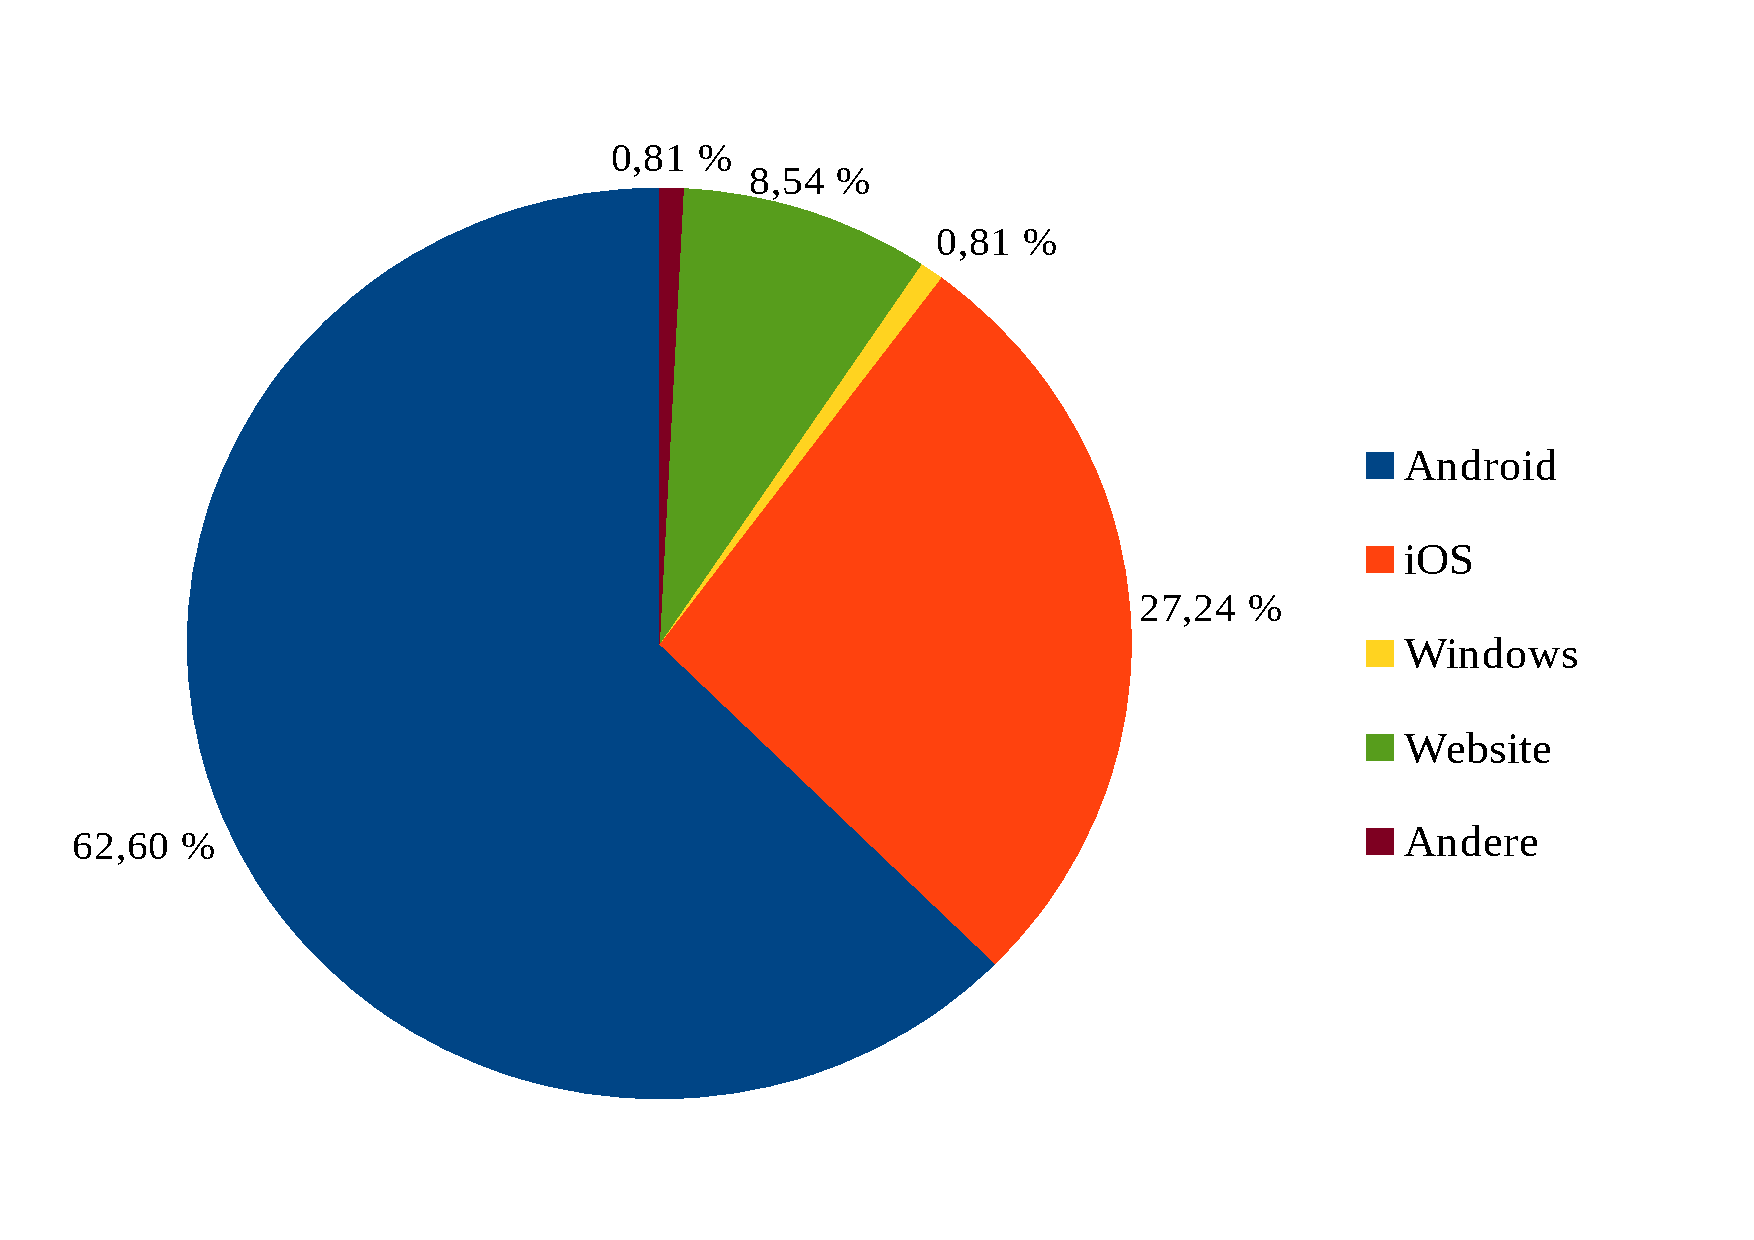
\includegraphics[width=12 cm]{Bilder/Umfrage/Umfrage_Appnutzung.pdf}
		\caption{Umfragewerte zur Nutzung der Apps nach Plattform\label{fig:umfrage_appnutzung}\protect\footnotemark}
	\end{center}
\end{figure}

\footnotetext{Brysiuk, Lehmann (2019)}

Wie man Anhand Abbildung \ref{fig:umfrage_appnutzung} erkennt, wird die Android \ac{App} der Hochschule Hof von 63\% der Studierenden mit Abstand am meisten genutzt, gefolgt von der \ac{iOS}-\ac{App} mit etwa 29\% aller Nutzer. Als letzte große Informationsquelle wird die Hochschul Website von etwa 6\% aller befragten Studierenden genutzt. Die Windows \ac{App} und andere Alternativen werden kaum genutzt. 

\subsection{Android}

Die Android \ac{App} der Hochschule Hof erfreut sich in den vergangenen Jahren großer Beliebtheit bei den Studierenden. Wie bereits gezeigt wurde, ist sie die meist genutzte \ac{App} aller Alternativen aus dem Hochschul Angebot. Neben den Grundfunktionen eines Stundenplans, eines personalisierten Stundenplans und dem Anzeigen der Stundenplanänderungen besitzt die \ac{App} im Vergleich zu den anderen nativen Anwendungen für \ac{iOS} und Windows die meisten zusätzlichen Funktionen. Unter anderem wurde eine Webview des Primuss Portal eingebaut, welche sich nach einem einmaligen Anmelden auch die Anmeldedaten des Nutzers merkt, was mehrfaches Einloggen unnötig macht. Ebenfalls durch eine Webview integriert wurde eine Navigation- und Fahrplanfunktion. Durch diese kann man sich Fahrzeiten und Verbindungen aller öffentlichen Verkehrsmittel anzeigen lassen. Weitere nützliche Funktionen sind die Raumsuche, \textit{Wo bin ich?} und die Chatfunktion für jede Vorlesung.
\\
\linebreak
%Speiseplan
Die Android \ac{App} der Hochschule Hof besitzt ebenfalls eine Schnittstelle, mit der sie Speiseplaninformationen aus dem Angebot des Studentenwerk Oberfrankens anzeigen kann. In dieser kann man seine Vorlieben speichern und sich nur die Speisen anzeigen lassen, welche für den Nutzer selbst relevant sind. Die Funktion ist besonders hervorzuheben, da nicht alle Anwendungen der Hochschule Hof das Menü des Studentenwerks bereitstellen. 

\subsection{iOS}

Mit knapp 29\% der befragten Nutzer liegt die \ac{iOS} Anwendung der Hochschule Hof an zweiter Stelle im Nutzungsranking der Umfrageteilnehmer. Das korreliert auch mit den allgemeinen Marktanteilen der Smartphone Betriebssysteme, welche in Abbildung \ref{fig:smartphoneOS_marktanteile} dargestellt werden\autocite[Vgl.][]{mobileosstatista}. Auch die Grundlegenden Funktionen des Stundenplans sind wie bei der Android \ac{App} vorhanden. Zusätzlich dazu hat der Nutzer die Möglichkeit, die offiziellen Termine der Hochschule Hof einzusehen, sowie eine eigene Aufgabenliste anzulegen und zu pflegen. Als kleinen Zusatz hat die \ac{iOS}-\ac{App} auch ein sogenanntes Widget. Das bedeutet, die Anwendung kann Daten auf dem Bildschirm des Smartphones anzeigen, ohne, dass die \ac{App} geöffnet ist.
\\
\linebreak
Zu bemängeln ist, dass die Nutzer dieser Anwendung keinen direkten Zugriff auf den Speiseplan der Mensa der \ac{HföD AIV} haben. Stattdessen haben befragte Nutzer angegeben, dass sie den Speiseplan über die offizielle Website des Studentenwerk Oberfrankens beziehen, sich aber eine Einbindung in die \ac{App} wünschen\autocite[][]{umfrage}.

\subsection{Windows App}

Die mit Abstand am wenigsten genutzte Anwendung der Hochschule Hof ist die Windows \ac{App}. Nur ein Prozent der befragten Studierenden nutzen demnach diese \ac{App}. Umgerechnet sind das lediglich 2 Nutzer. Trotz der geringen Nutzung bietet die Windows Anwendung ein sauberes Interface, über welches der Nutzer die üblichen Informationen wie die anstehenden Vorlesungen einsehen kann. Auch hier hat der Anwender die Möglichkeit, seinen Stundenplan zu personalisieren. Weitere nützliche Funktionen sucht man hingegen vergeblich. Im Gegensatz zur \ac{iOS}-\ac{App} bietet die Windows \ac{App} dennoch die aktuellen Speiseplan Informationen an.

\subsection{Website}

Als Alternative zur Nutzung der nativen, plattformabhängigen und unabhängig entwickelten Anwendungen der Hochschule Hof soll hier nochmals die Website als Informationsquelle für Stundenplaninformationen und weitere nützliche Daten betrachtet werden. Die Nutzergruppe, die keine der Smartphone \acp{App} nutzt macht immerhin fast 6\% aus und ist damit deutlich größer als die der Windows User.
\\
\linebreak
Stundenplan Informationen können nach einer einfachen Auswahl des Studiengangs und des Fachsemesters eingesehen werden. Weitere Verfeinerungen der Vorlesungen bietet die Art der Veranstaltung, welche die Trefferliste eingrenzt. Zusätzlich bietet die Seite die Möglichkeit an, den Stundenplan als \ac{PDF} herunterzuladen und zu drucken. Ähnlich werden auch die Stundenplanänderungen angezeigt. Nach Auswahl des Studiengangs und des Fachsemesters werden dem Nutzer alle anstehenden Änderungen angezeigt. Zusätzlich kann der Nutzer auch ein Datum angeben, um die Ergebnisse zu filtern.
\\
\linebreak
Um den Mensa Speiseplan des Studentenwerk Oberfrankens mit einzubinden, wurde der Website ein Verweis auf die offizielle Website des Anbieters hinzugefügt. Dieser leitet allerdings nur auf die offizielle Website weiter und bietet keine weiteren Informationen.

\subsection{Fazit}

Im Allgemeinen kann man erkennen, dass die Nutzungsverteilung der \acp{App} der Hochschule Hof mit den Marktanteilen der Smartphone Betriebssysteme in Deutschland korreliert. Dies ist besonders gut in Abbildung \ref{fig:smartphoneOS_marktanteile} zu erkennen\autocite[][]{mobileosstatista}. Da die meisten der Studierenden ein Android betriebenes Handy besitzen, wird diese \ac{App} auch am meisten genutzt. Genauso lässt sich die Nutzung der \ac{iOS}-\ac{App} erklären. 

\begin{figure}[h]
	\begin{center}
		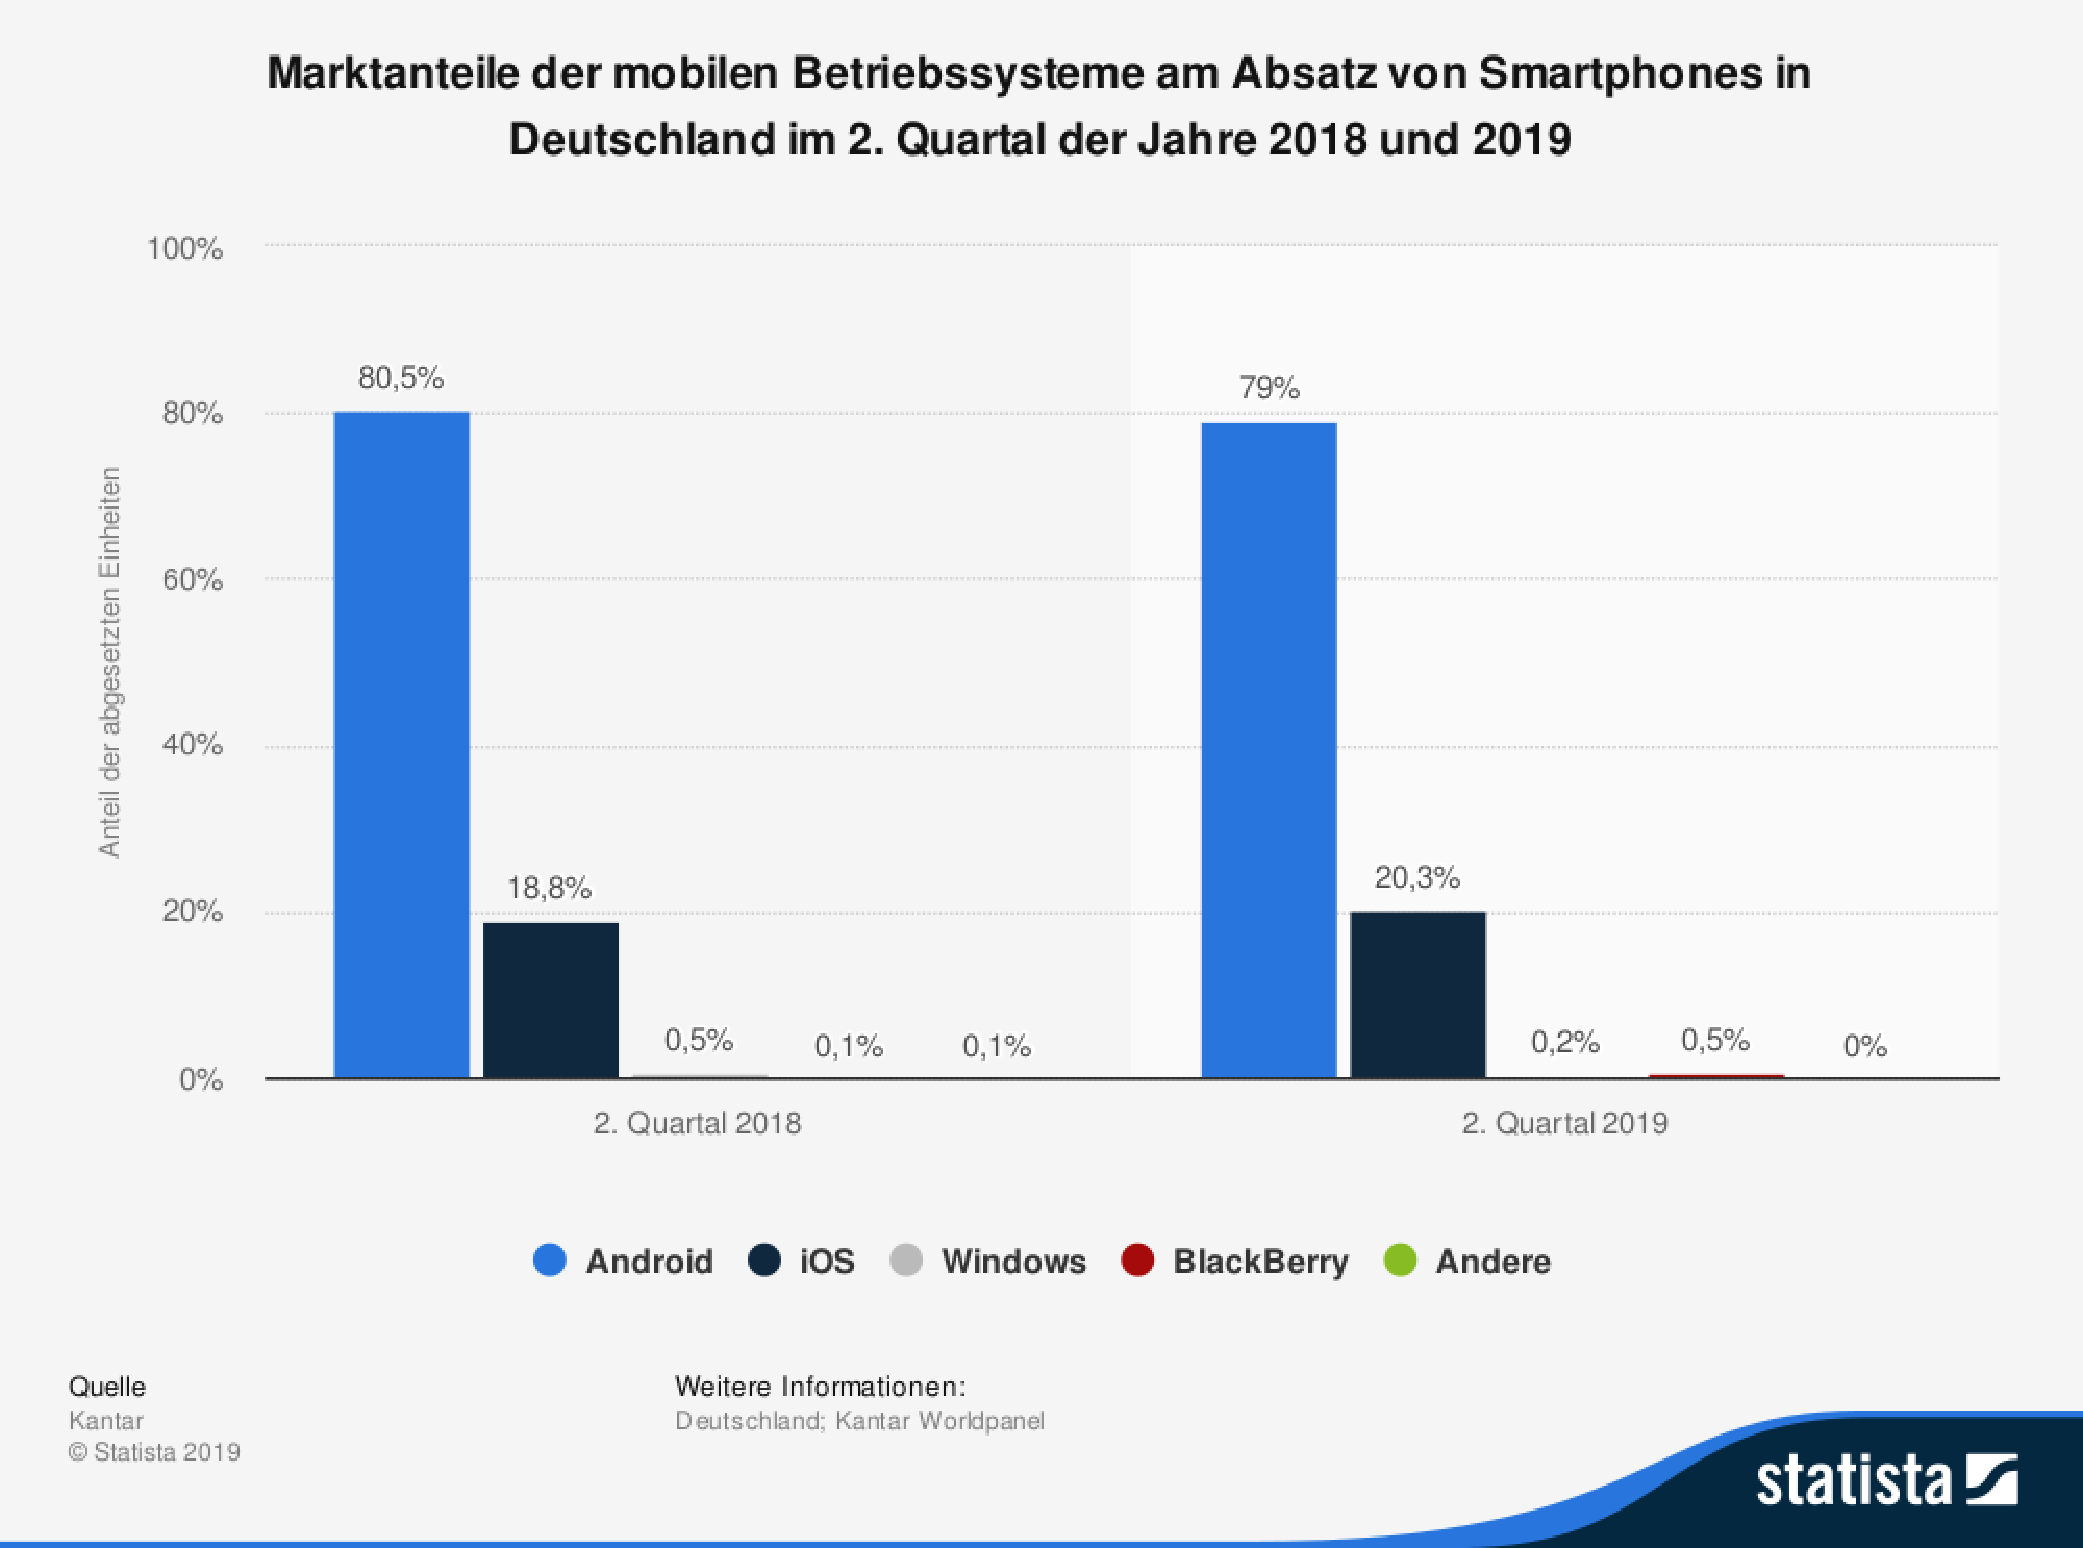
\includegraphics[width=12cm]{Bilder/Statistik/Statista_SmartphoneOS.pdf}
		\caption{Marktanteile der mobilen Betriebssysteme am Absatz von Smartphones in Deutschland im 2. Quartal der Jahre 2018 und 2019\label{fig:smartphoneOS_marktanteile}\protect\footnotemark}
	\end{center}
\end{figure}
\footnotetext{ebd.}

%Kantar. (2019). Marktanteile der mobilen Betriebssysteme am Absatz von Smartphones in Deutschland im 2. Quartal der Jahre 2018 und 2019. Statista. Statista GmbH. Zugriff: 15. August 2019. https://de.statista.com/statistik/daten/studie/198435/umfrage/marktanteile-der-smartphone-betriebssysteme-am-absatz-in-deutschland/

Dennoch ist anzumerken, dass die Android Version die meisten zusätzlichen Features bietet, auch wenn sie laut Nutzerberichten nicht zuverlässig funktionieren und oft auch nicht als sinnvoll eingestuft werden\autocite[Vgl.][]{umfrage}. Auch die Einbindung der Speiseplan-Informationen ist eine gern gesehene Funktion bei den Studierenden und wird demnach auch bei den Nutzern der \ac{iOS}-\ac{App} gefordert.

% Anforderung
\chapter{Funktionale Anforderungen}
\label{sec:anforderung}
% Text

Um eine solide Grundlage für die Entwicklung einer Anwendung zu haben, benötigt es ein Lastenheft, das vor dem Entwicklungsprozess definiert werden muss. Die oberste Priorität in einem solchen Lastenheft haben die Anforderungen des eigentlichen Auftraggebers. Zusätzlich wurden nach Wunsch des Auftraggebers noch weitere Anforderungen aus dem International Office und dem Sprachenzentrum gesammelt. Diese zwei Teile des Lastenhefts richten sich nach einer der Säulen des Leitbilds der Hochschule Hof, der Internationalisierung mit Fokus auf Indien. Im folgenden werden die gesammelten Anforderungen an die web-basierte Hochschul-\ac{App} genauer betrachtet.

\section{Auftraggeber\label{sec:anforderungen_ag}}

In den vergangenen Jahren wurden die Anwendungen der Hochschule Hof durch verschiedene Professoren und Mitarbeiter der Hochschule Hof beaufsichtigt und geleitet. Im vergangenen Sommersemester 2019 ist die Zuständigkeit der Android \ac{App} an Prof. Dr. Heym übergegangen. Statt sich jedoch auf die plattformabhängige Version zu fixieren strebt dieser es stattdessen an, eine betriebssystemunabhängige Anwendung zu schaffen, die auf allen Endgeräten funktioniert und dennoch für mobile Endgeräte optimiert ist.

\subsection{Grundlegende Anforderung}
%urspr. Allgemeines

Der Fokus soll in der kommenden \ac{App} darauf liegen, dass sie für alle Anwender gleich nutzbar ist, unabhängig davon, welches Endgerät genutzt wird, ob \ac{PC}, Smartphone oder Tablet. Auch das Betriebssystem soll dabei keine Rolle mehr spielen. Zudem ist ein großer Beweggrund für diese Arbeit die Neuentwicklung einer Anwendung, welche durch die gesammelten Erfahrungen der \acp{App} der vergangenen Jahre an die Bedürfnisse der Nutzer angepasst wird.  

\subsection{Funktionale Anforderungen}

Im folgenden werden die Anforderungen und deren Gewichtungen aufgeführt und näher erläutert.

\subsubsection{Stundenplan}

Wie in allen Anwendungen der Hochschule Hof ist die zentrale Funktion der \ac{App} das Anzeigen des Stundenplans. Dieser Stundenplan soll sich allgemein nach dem Studiengang und dem Fachsemester des Anwenders richten. Zusätzlich soll es einen personalisierten Stundenplan geben, den sich der Nutzer eigenständig zusammenstellen kann. Anders als in den bereits vorhandenen Anwendungen soll der Fokus des Stundenplans auf der Personalisierung liegen. 
\\
\linebreak
Hierbei soll auf folgende Punkte geachtet werden:

\begin{itemize}
	\item Fakultät des Nutzers
	\item Studiengang des Nutzers
	\item Fachsemester des Nutzers
	\item Einfache Einbindung nicht regulärer Vorlesungen
	\item Einfache Einbindung des erweiterten Vorlesungsspektrums der Hochschule (z.B. Sprachkurse)
\end{itemize}

\subsubsection{Stundenplan Änderungen}

Zusätzlich zu den allgemeinen Stundenplan Informationen und der personalisierten Ansicht sollen auch die Änderungen im Vorlesungsprogramm dargestellt werden. Hierbei ist zwischen langfristigen Änderungen und den einmaligen Änderungen zu unterscheiden. Langfristige Änderungen könnten zum Beispiel dauerhafte Raumänderungen, Wechsel des Dozenten oder die Absage einer Veranstaltung sein. Diese sollten automatisiert angepasst werden, wobei dem Nutzer einmalig mitgeteilt werden soll, dass sich diese Veranstaltung geändert hat. Kurzfristige Änderungen hingegen sind Änderungen, welche Einmalig eintreten. Darunter fallen zum Beispiel einmalige Raumänderungen, Ausfälle durch Verhinderung des Dozenten oder Verschiebungen von Vorlesungen. Diese sollten möglich klar in die Ansicht des Stundenplans fallen, sodass der Nutzer sofort erkennt, dass der aktuelle Zeitplan vom Regelfall abweicht. Zusätzlich soll der Anwender benachrichtigt werden, wenn sich eine Änderung ergibt.

\subsubsection{Speiseplan}

Wie auch in den Anwendungen für Android und Windows soll die neue \ac{App} die Speiseplan Informationen des Studentenwerk Oberfrankens anzeigen. Diese Informationen sollen nach den Wünschen des Anwenders gefiltert werden. Demnach kann sich der Anwender alle Preiskategorien anzeigen lassen oder eben nur die Kategorie, in die er selber auch fällt. Zudem soll standardmäßig das ganze Menü angezeigt werden. Stattdessen soll der Nutzer auch einige Teile des Menüs ausblenden können. So kann ein vegetarischer Nutzer zum Beispiel nur die vegetarischen Gerichte anfordern. Weiterhin sollen die Speisen mit allen zusätzlichen Informationen angezeigt werden, wie zum Beispiel den Inhaltsstoffen und Allergenen.

\subsubsection{Anwenderverwaltung}

Um die weiter oben erwähnten personalisierten Darstellungen der Stundenplan und Speiseplan Informationen anbieten zu können, ohne dass sie bei jeder Öffnung der Anwendung neu eingestellt werden müssen, ist es notwendig, dass eine Anwenderverwaltung implementiert wird. Diese kann dann die nötigen Einstellungen der Nutzer speichern. Diese Anwenderverwaltung soll jedoch so flexibel wie möglich bleiben. Im Fokus stehen nach wie vor die Studierenden der Hochschule Hof, die eine E-Mail-Adresse der Hochschule besitzen. Jedoch ist dies nicht immer der Fall. Die Nutzergruppe der Anwendung kann folgende Studierende enthalten:

\begin{itemize}

\item Reguläre Studierende

\item Gaststudierende

\item Sprachkurs Teilnehmer

\item Internationale Studierende

\end{itemize}

Gaststudierende und Teilnehmer der Sprachkurse sind nicht immatrikuliert und haben demnach auch keine E-Mail-Adresse der Hochschule Hof. Dennoch belegen sie Kurse und sollen einen personalisierten Stundenplan erstellen können. Deshalb ist es wichtig, dass auch sie im Bereich der Anwenderverwaltung berücksichtigt werden. 
\\
\linebreak
Um nicht unnötig Daten zu sammeln und die Nutzer, die nicht mehr an der Hochschule studieren aus der Anwenderverwaltung zu entfernen ist es auch wichtig, dass Nutzerdaten automatisiert gelöscht werden, wenn sie nicht mehr benötigt werden oder der zugehörige Nutzer nicht mehr berechtigt ist, sich anzumelden. Diese Anforderung wird jedoch im Laufe dieser Arbeit nicht weiter betrachtet. Stattdessen wird auf die parallel dazu erstellte Bachelorarbeit zur Authentifizierung und Personalisierung verwiesen\autocite[][]{andreasba}.

\subsubsection{Mehrsprachigkeit}

Neben dem International Office stellt auch der Auftraggeber die Anforderung, die Daten der Anwendung in mehreren Sprachen bereitzustellen. Unter diesen Sprachen sollte demnach mindestens Deutsch und Englisch sein. Das Ziel dieser Anforderung ist es, die Internationalen Studierenden besser zu unterstützen.

\subsubsection{Mobile First}

Wie bereits erwähnt wurde, soll die Anwendung Plattform unabhängig sein. Demnach muss es egal sein, welches Endgerät der Anwender nutzt, um die \ac{App} aufzurufen. Ebenfalls egal ist das Betriebssystem, das auf dem Endgerät installiert ist. Jedoch soll die Anwendung, auch wenn sie sich auf allen Endgeräten gleich verhalten muss, auf mobile Endgeräte angepasst sein. Das bedeutet, dass die Informationsdarstellung und die Navigation primär auf mobilen Endgeräten einfach zu bedienen sein muss. Weiterer Implementierungsaufwand kann dann nach Bedarf noch in die 
dynamische Anpassung an den Client investiert werden.

\section{International Office\label{sec:anforderungen_io}}

Die Hochschule Hof hat sich im Laufe der vergangenen Jahre immer mehr mit dem Thema Internationalisierung auseinandergesetzt. Aus diesem Grund wurde die Internationalisierung mit Fokus auf Indien im Frühjahr 2011 sogar als zentrale Säule in das Leitbilds der Hochschule Hof aufgenommen\autocite[Vgl.][]{campuls}.
\\
\linebreak
Konkret heißt es im Leitbild der systemakkreditierten Hochschule Hof\autocite[Vgl.][]{fhhofwebsite}:
\begin{quote}
Der Erfolg der Absolventen in nachhaltig wirtschaftenden und international agierenden Unternehmen bestimmt das Handeln aller Mitglieder des wissenschaftlichen Unternehmens Hochschule Hof. Die Studierenden werden in unserer  weltoffenen Green Tech University exzellent betreut. Praxisorientierte, international ausgerichtete und der Ressourceneffizienz verpflichtete Aus- und Weiterbildung prägt unsere Arbeit. Die angewandte Forschung sichert die Aktualisierung des Wissens für die Lehre und entwickelt Lösungen zum Nutzen für die Wirtschaft.
\end{quote}
Klar zu erkennen ist hier die mehrmalige Erwähnung der Internationalisierung der Hochschule Hof. Aus diesem Grund wird im Laufe der Neuentwicklung einer Hoch\-schul-\ac{App} auch mit dem International Office der Hochschule Hof zusammengearbeitet.

\subsection{Problem}

Wie bereits im Kapitel \ref{umfrage_zielgruppen} beschrieben wurde, ist eine der Nutzergruppen der Hochschul-Anwendungen die der internationalen Studierenden der Hochschule Hof. Durch Sprachbarrieren und andere Kommunikationsschwierigkeiten, sowie durch fehlende oder nur schwer auffindbare auf englisch verfasste Informationen, fällt es diesen schwer das volle Informationsangebot der Hochschule Hof zu nutzen. Auch die Nutzung der hochschuleigenen \acp{App} ist davon betroffen, denn viele Internationale Studierenden sind mit dem Funktionsumfang der angebotenen Anwendungen unzufrieden. 

\subsection{Funktionale Anforderungen\label{sec:anf_io}}

Den oben genannten Gründen zufolge werden folgende Anregungen und Anforderungen des International Office mit in die Analyse der verbesserten Hochschul-\ac{App} aufgenommen und im Entwicklungsprozess berücksichtigt.

\subsubsection{Spracherweiterung}

Die wohl einfachste Anforderung, die sich aus den Gesprächen mit dem International Office ergeben, ist die, zukünftige Anwendungen nicht nur in deutscher Sprache anzubieten, sondern auch in anderen Sprachen, allen voran Englisch. Englisch wurde beispielsweise von etwa 23\% der gesamten Befragten als weitere Sprache erwünscht, während sowohl Spanisch als auch Indisch jeweils von 20\% der Befragten angegeben wurde. Auch Französisch besitzt mit 14\% einen hohen Zuspruch unter den befragten Studierenden. 

\begin{figure}[h]
	\begin{center}
		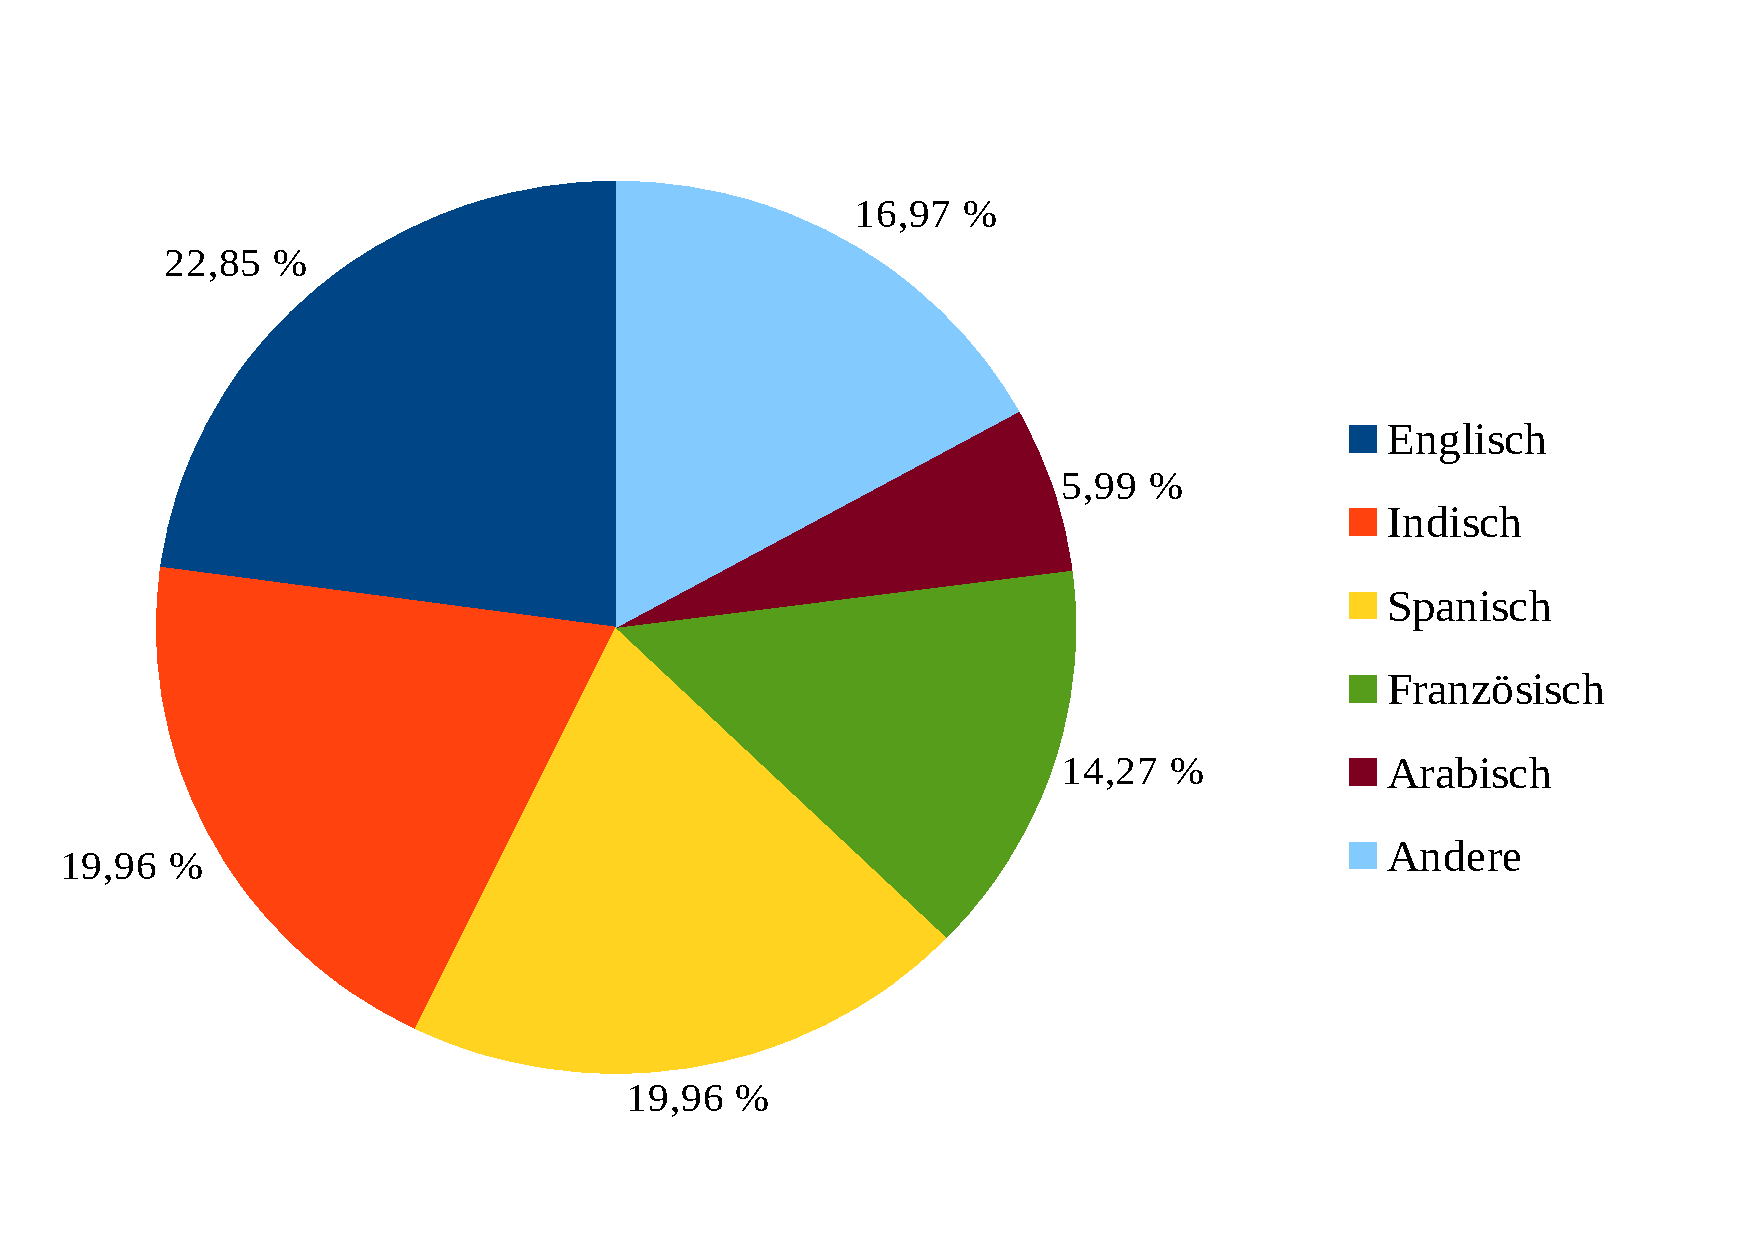
\includegraphics[width=12cm]{Bilder/Umfrage/Umfrage_Sprachen.pdf}
		\caption{Umfragewerte zu gewünschten Spracherweiterungen\label{fig:umfrage_sprachen_diagram}\protect\footnotemark}
	\end{center}
\end{figure}

\subsubsection{Einfachere Stundenplanerstellung}


\footnotetext{Brysiuk, Lehmann (2019)} %auf richtiger Seite wie grafik???

Aus den Gesprächen mit dem International Office der Hochschule Hof hat sich ergeben, dass viele Internationale Studierende große Probleme damit haben, einen vollständigen Stundenplan über eine der \acp{App} zu pflegen. Das liegt vor allem daran, dass viele der Internationals Vorlesungen aus verschiedenen Studiengängen und teilweise sogar aus verschiedenen Fakultäten belegen. Es ist zwar prinzipiell möglich, einen solchen Stundenplan in den \acp{App} zu erstellen, allerdings ist dies nicht einmal vorgesehen und funktioniert so nur durch Zufall. Die internationalen Studierenden, die sich bei der Bedienung der Anwendungen ohnehin schon schwer tun, finden solche Schlupflöcher einfach nicht und befinden die \acp{App} somit als unbrauchbar. Das International Office wünscht sich deshalb, das die personalisierte Stundenplanzusammenstellung in den Anwendungen oder in einer neuen Anwendung deutlich flexibler wird.  

\section{Sprachenzentrum\label{sec:anforderungen_sz}}

Die Hochschule Hof bietet neben ihren regulären Veranstaltungen, die durch die Fakultäten organisiert und gehalten werden, ebenfalls eine reiche Auswahl an Sprachkursen an. Diese werden vom Sprachenzentrum der Hochschule Hof veranstaltet. Die hohe Bedeutung von gut organisierten Sprachkursen an einer akademischen Institution ist unbestreitbar. Das Sprachenzentrum selbst formuliert es wie folgt:
\begin{quote}
Sprachen sind das Tor zur Welt; unerlässlich in einer akademischen Karriere. Daher wird an der Hochschule Hof als international ausgerichteter Hochschule besonderer Wert auf eine profunde Sprachausbildung gelegt.
\autocite[][]{szweb}
\end{quote}
Konkret werden aktuell an der Hochschule Hof allgemeine Sprachkurse in den Sprachen Englisch, Spanisch, Französisch, Chinesisch, Russisch, Türkisch sowie Deutsch angeboten. Diese werden im Rahmen von Pflicht- und Wahlveranstaltungen für Studierende, sowie als \ac{UNIcert}-Prüfungen und \ac{TestDaF} angeboten.
\\
\linebreak
Jedoch bringt das Angebot von zusätzlichen Veranstaltungen, die nicht von den Fakultäten organisiert werden, einige Herausforderungen mit sich. Diese werden im folgenden aufgelistet, wobei mögliche Lösungen im Rahmen dieser Bachelorarbeit erörtert werden.

\subsection{Problem\label{sec:prob_sz}}

Das Ziel der Hochschule Hof ist es, den Studierenden einen einfachen und übersichtlichen Zugang zu den benötigten Informationen des Sprachenzentrums zu geben. Vor allem bei den internationalen Besuchern der Vorlesungen ist es wichtig, dass sie das Angebot der Sprachkurse leicht einsehen können, denn für sie sind deutsche Sprachkurse oft verpflichtend. Aber auch reguläre Studierende belegen oft Sprachkurse, entweder, um ihre Kenntnisse aus vorangegangenen Kursen zu vertiefen oder um sich neue Sprachen anzueignen. So geben etwa 89\% der deutschsprachigen Studenten an, dass sie Informationen zum Sprachenzentrum gerne mit in eine allgemeine Hochschulanwendung eingebunden hätten. Auffällig ist hier auch die Statistik bei den nicht deutschsprachigen Studierenden. Hier sind es bereits 93\%, die eine Erweiterung der aktuellen Anwendungen mit dem Angebot an Sprachkursen begrüßen würden. Hier hilft oft auch die Nutzung der Website nicht weiter. Somit sind zum Aufrufen allgemeiner Infos des Sprachzentrums bereits fünf Klicks von der Startseite aus gezählt nötig, für Änderungen im Kursprogramm sind es sogar schon sechs\autocite[][]{umfrage}.
\\
\linebreak
Für die internationalen Studierenden ist hier die Informationssuche deutlich schwieriger, da diese Informationen im englischen Angebot des Sprachenzentrums auf der Hochschul Website nicht aufgeführt werden. Zudem ist die Informationsbeschaffung der Studenten in Bezug auf die Sprachkursinformationen im Vergleich zu den fachbezogenen Vorlesungen deutlich unterscheidbar. In der Android \ac{App} ist das Sprachenzentrum beispielsweise als eigener Studiengang geführt und kann nur so in den Stundenplan aufgenommen werden. Dies kann bei vielen Studierenden zu Verwirrung führen. Andere Nutzer kennen diesen Spezialfall in der Implementierung der Anwendung nicht und können die Stunden ihrer Sprachkurse somit auch nicht in ihren persönlichen Stundenplan aufnehmen. Zudem sind Sprachkursinformationen, sowohl allgemeine Informationen als auch Stundenpläne zu dem Kursangebot, auf der Website der Hochschule separat geführt. Somit ist die Suche nach den Sprachkursen, die ein Studierender nutzen möchte, mit einem deutlichen Mehraufwand gegenüber der regulären Vorlesungssuche verbunden. 

\subsection{Funktionale Anforderungen\label{sec:anf_sz}}

Aus den oben genannten Problemen der aktuellen Informationsdarstellung ergeben sich einige Anforderungen an eine neue Hochschul-\ac{App}, welche nun weiter erörtert werden.

\subsubsection{Einbinden von Sprachkursinformationen}

Eine Anforderung des Sprachenzentrums ist es, die Informationen, die es anbietet, in eine Hochschul-\ac{App} einzubinden. Der Fokus sollte darauf liegen, das Sprachangebot der Hochschule wie normale Vorlesungen zu behandeln, zu denen die Studierenden ebenfalls alle relevanten Informationen abgreifen können.

\subsubsection{Mehrsprachige Sprachkursinformationen}

Des weiteren ist es wünschenswert, die Informationen des Sprachenzentrums nicht nur in deutscher Sprache, sondern auch in Fremdsprachen, vor allem in Englisch, einzubinden. Dabei sollte der Fokus nicht nur auf allgemeinen Informationen liegen, sondern auf spezielleren Daten, wie Details zu Stundenplanänderungen im Bereich der Sprachkurse. 

\subsubsection{Einheitliche Darstellung}

Es ist wünschenswert, dass die Sprachkurse im selben Rahmen wie die regulären, verpflichtenden Vorlesungen der Studierenden dargestellt werden. Es sollte also möglich sein, die belegten Sprachkurse genauso leicht in einen personalisierten Stundenplan zu übernehmen, wie die regulär belegten Vorlesungen. 

\subsubsection{Vollständige Informationsdarstellung}

Zu den Sprachkursen sollten nicht nur allgemeine Informationen wie Veranstaltungsort und Zeitpunkt stehen, stattdessen fordert das Sprachenzentrum die genauere Einbindung einiger Details. Eines dieser Details sind die Sprachniveaus der angebotenen Kurse. Werden diese angezeigt, ist es auch wichtig, dass ersichtlich ist, ob ein Kurs einen sogenannten Placementtest benötigt, der die Studierenden zur Teilnahme am Kurs berechtigt.
 
\subsubsection{Vorgeschlagene Features}

Das Sprachenzentrum hat des weiteren einige Vorschläge zur Verbesserung der Nutzbarkeit einer neuen Anwendung erbracht. 
%1
Einer dieser Ideen ist die Möglichkeit, bei der Auswahl eines Sprachkurses in einen personalisierten Stundenplan direkt zu der Anmeldung dieses Kurses weitergeleitet zu werden.
%2
Zudem kann es hilfreich sein, angebotene Sprachkurse nach deren Niveau filtern zu können.
%3
Ebenso kann eine verbesserte Hochschul-\ac{App} dem Nutzer auch die angebotenen Sprachkurse anzeigen, die in den freien Stunden seines personalisierten Stundenplans angeboten werden. So kann er die Freizeit zwischen seinen Pflichtveranstaltungen sinnvoll nutzen und die Sprachkurse werden optimal ausgelastet.

\section{Pflichtenheft\label{sec:pfilchtenheft}}

Die in Kapitel \ref{sec:anforderung} gesammelten Anforderungen können für das Projekt der neuen Hoch\-schul-\ac{App} als Lastenheft angesehen werden. Dieses wird benötigt, um klar definieren zu können, was der Auftraggeber und andere Interessenparteien von einem Projekt erwarten. Was ein Lastenheft jedoch nicht definiert ist der Rahmen und Umfang der Anforderungen, die auch im späteren Implementierungsprozess umgesetzt werden. Dafür muss vor der Implementierung noch ein Pflichtenheft definiert werden. Die darin definierten Pflichten sind dann genau die Anforderungen, die im Rahmen der zu dieser Bachelorarbeit parallel geführten Praxisarbeit umgesetzt werden\autocite[Vgl.][]{dnpa}. Um das Lastenheft und das Pflichtenheft klar voneinander trennen zu können wird das Pflichtenheft in der eben genannten Praxisarbeit definiert. Eine Gegenüberstellung der geplanten und umgesetzten Anforderungen kann dann anhand der Referenznummern  aus dem Lastenheft erfolgen. Das Lastenheft kann dem Anhang dieser Arbeit entnommen werden.


% Ausarbeitung der Architektur
\chapter{Architektur von Softwaresystemen}
\label{sec:softwarearchitektur}

Die virtuelle Welt wächst immer schneller und schneller, die Digitalisierung ist mitten im Gange. Schlagzeilen über Industrie 4.0, \ac{IoT}, Cloud, Block Chain, \ac{DevOps}, BigData oder \ac{AI} tauchen immer öfter in den digitalen Nachrichten Welt auf. Viele Unternehmen setzten sich das Ziel, deren Strukturen zu modernisieren, so wie die Unternehmensprozesse zu optimieren. Diese sollen flexibler, schneller und effizienter ablaufen. Doch auch Privatpersonen rüsten stark nach, ein Leben ohne Smartphone ist heutzutage kaum noch vorstellbar. Navigation, Kommunikation, Unterhaltung, Shopping, Banking und vieles mehr damit sind möglich, ein Gerät für alle Fälle. Allein im zweiten Quartal des Jahres 2019 stehen über 4.5 Millionen Anwendungen für sogenannte Smartphones zur Verfügung und es werden täglich immer mehr\autocite[Vgl.][]{appstore}.
%Appfigures. (2019). Anzahl der verfügbaren Apps in den Top App-Stores im 2. Quartal 2019. Statista. Statista GmbH. Zugriff: 26. August 2019. https://de.statista.com/statistik/daten/studie/208599/umfrage/anzahl-der-apps-in-den-top-app-stores/

Der Wandel unter dem Schlagwort \textit{Digitale Transformation} hat natürlich auch gravierende Auswirkungen auf die Systemarchitekturen. Denn die Bauweisen solcher Systeme sollen Zukunftsfähig sein, obwohl dies nicht so einfach ist, schon allein weil heute noch nicht bekannt ist, was morgen neu erscheinen wird. Die Gefahr besteht darin, dass viele der aktuellen \ac{IT}-Systeme in ihrer Existenz bedroht wären, wenn sie keine grundlegende Modularisierung vorweisen könnten. Genau deshalb muss das Ziel der modernen \ac{IT}-Entwickler sein, deren Systemarchitekturen so zu gestalten, dass eine möglichst hohe Modularität und Flexibilität eine Grundlage deren wird\autocite[Vgl.][17\psq]{gmodse}.


Die Modularisierung ermöglicht die Beherrschung der \textit{digitalen Transformation}. Dadurch entstehen Flexibilitätsvorteile, die die ideale Reaktion auf das dynamische Wachstum der Digitalisierung ist. Somit handelt es sich beim Thema Modularisierung um eine der wichtigsten Konzepte der Softwarearchitektur. Die Modularisierung eines \ac{IT}-Systems ist erfüllt, wenn das gesamte \ac{IT}-System in einzelne Komponente zerlegt werden kann. Jede einzelne Komponente ist als abgegrenzter Teil des Systems definiert und übernimmt eine entsprechende Funktionalität des \ac{IT}-Systems. 

Die einzelnen Komponenten sollten möglichst unabhängig voneinander sein und zudem die einfache Ersetzbarkeit durch eine andere Komponente mit denselben Eigenschaften ermöglichen. Auch bei einem Ausfall einer der Komponenten wird das System weiterhin funktionieren, dann eben ohne die Funktionalität der ausgefallenen Komponente.

Die Zerlegung in einzelne Komponenten bieten folgende Vorteile\autocite[Vgl.][3\psq]{gmodse}:
\begin{itemize}
\item Diese können ohne Seiteneffekte und Abstimmungsarbeit weiterentwickelt werden.
\item Diese können unabhängig von Rest dokumentiert und verstanden werden.
\item Diese können an ihren ein- und ausgehenden Schnittstellen isoliert getestet werden.
\item Diese können leicht ausgetauscht werden.
\item Diese sind flexibel an das Wachstum des \ac{IT}-Systems anpassbar.
\item Diese reduzieren die Komplexität des \ac{IT}-Systems.
\end{itemize}

\begin{quote}
\glqq{}Sollte eine Software mit der Zeit irgendwelche Probleme bekommen, sei es beispielsweise mit der Stabilität oder mit der Wartbarkeit, so werden sich diese Probleme, so man auch immer auf Modularisierung geachtet hat, immer nur auf einen Teil des Systems beziehen und niemals auf die gesamte Software. Software ab einer gewissen Größenordnung, die keine erkennbaren Strukturen aufweist, kommt potenziell in existenzielle Bedrohung, sobald sie die ersten Probleme dieser Art aufweist.\grqq{} \footnote{a.a.O., S. 3.}
\end{quote}

Ein ausgezeichnetes Negativbeispiel dafür sind die aktuellen Hochschul-\acp{App}. Diese wurden für jedes System separat Entwickelt und das nur mit genau den Funktionalitäten, die zu dieser Zeit erforderlich waren. Somit hat jedes \ac{IT}-System eine eigene Softwarearchitektur bekommen und die Funktionalitäten wurden für jedes System auf eine andere Art und Weise implementiert. Jedoch sind durch die bereits erwähnte Digitalisierung über die Jahre immer neue Anforderungen an die \ac{IT}-Systeme entstanden. Diese wurden bereits ausführlich in Kapitel \ref{sec:anforderung} beschrieben. Durch die nicht modularisierte Gestaltung der Softwarearchitektur der bestehenden \ac{IT}-Systemen ist die Entwicklung bei einem Punkt angekommen, bei der gemeinsame Erweiterungen oder Änderungen der Anwendungen für alle \ac{IT}-Systeme entweder aufwändig oder sogar nicht möglich sind.
\\
\linebreak
Somit handelt es sich bei der Erstellung einer Softwarearchitektur um eine der wichtigsten Disziplinen in der \ac{IT}-Branche. Zu beachten ist jedoch, dass die Softwarearchitektur nicht nur aus dem Drang nach Modularität besteht, denn es müssen noch viele andere wichtigen Anforderungen und Prinzipien eingehalten werden, um eine zukunftsfähige Softwarearchitektur zu erstellen. Auf diese Anforderungen und Prinzipien wird in den nächsten Kapiteln eingegangen. Außerdem muss berücksichtigt werden, dass nur modulare Softwarearchitekturen in Frage kommen, denn das Ziel dieser Bachelorarbeit ist es, eine erweiterbare, betriebssystemunabhängige Hochschul-\ac{App} zu entwickeln.


\section{Grundlegendes}
Die Realisierung eines jeden Projekts benötigt immer einen ersten Architekturentwurf. Egal welche Industriezweige es betrifft, ob der Bau einer Brücke geplant werden soll, ein Netzwerk umgesetzt werden muss oder eine Anwendung implementiert werden soll, am Anfang steht immer die Architektur. Ein früher Entwurf, der später noch detaillierter beschrieben werden kann, bietet anfangs eine gute Grundlage für vorzeitige Bewertungen und Entscheidungen zur Verteilung der Ressourcen. Außerdem lassen sich oft vorzeitig Probleme erkennen und schneller beheben.
\\
\linebreak
Beim Entwurf einer Anwendung werden die Spezifikationen der einzelnen Funktionalitäten in Komponente zerlegt um die Komplexität weitgehend nach dem Prinzip \textit{teile und herrsche} zu minimieren. Dabei wird der Aufbau der benötigten Teilsysteme, sowie die Festlegung der Verbindungen und Abhängigkeiten der Komponenten untereinander, beschrieben. Jedoch besteht eine Softwarearchitektur nicht nur aus der Anwendung selbst. Stattdessen müssen auch andere Schichten beachtet werden, um einerseits die nicht-funktionalen Anforderungen abzudecken und andererseits die Anpassung an die Umgebung, auf dem die Anwendung später implementiert werden soll, zu gewährleisten. Zudem muss auch auf die nötige Middleware eingegangen werden, die benötigt wird, um mit externen Systemen kommunizieren zu können. Somit ist die Entscheidung des Software-Designs einer der wichtigsten Punkte bei Erstellung einer Anwendung\autocites[Vgl.][]{onlinelexikonsa}[Vgl.][1]{gmodse}.

\section{Nicht-funktionale Anforderungen}
\label{sec:nfa}
Die nicht-funktionale Anforderungen sind meistens die Anforderungen, die nicht explizit vom Auftraggeber erwähnt werden, sondern die, die sich eher automatisch aus den Vorgaben ergeben oder die man bei aktueller Software als selbstverständlich sieht. Die meisten solcher Anforderungen sind in Abbildung \ref{fig:anforderungen} zu sehen.

\begin{figure}[H]
\centering
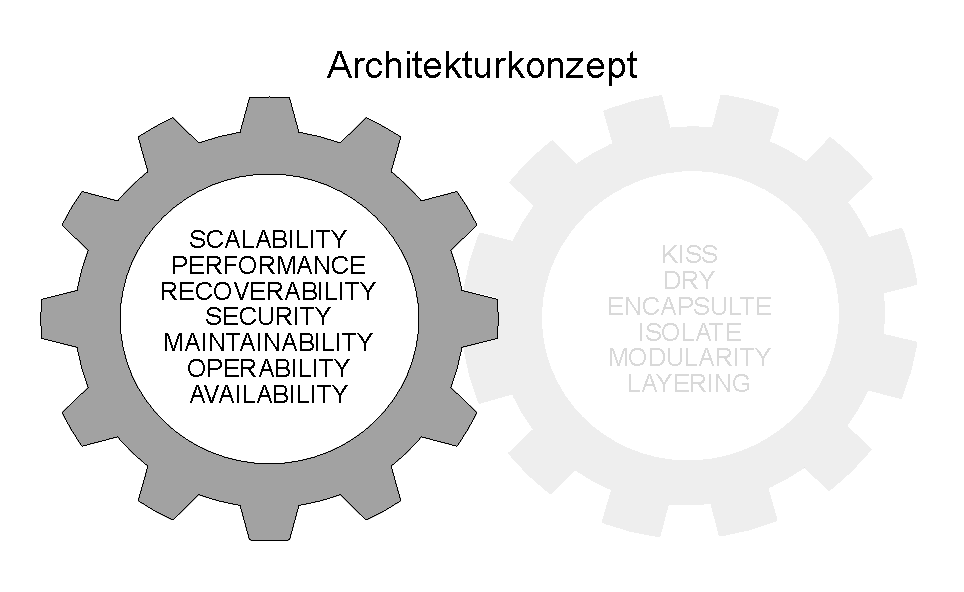
\includegraphics[width=\pictureWidth cm]{Bilder/Sonstiges/Anforderungen_Prinzipien-Transparent.pdf}
\caption{Allgemeine Anforderungen an eine Architektur\label{fig:anforderungen}\protect\footnotemark}
\end{figure}
\footnotetext{Brysiuk, Lehmann (2019)}

Es ist bei einem Softwareentwurf immer wichtig, sich über alle nicht-funktionalen Anforderungen Gedanken zu machen, denn diese bilden den Grundbaustein für eine erfolgreiche und zukunftsfähige Anwendung. Dadurch können spätere Mängel leichter behoben werden, neue Anforderungen schneller umgesetzt werden und die Anwendung an das Wachstum der Hochschule angepasst werden.

\section{Prinzipien}
\label{sec:prinzipien}

Ein weiterer wichtiger Punkt ist die Beachtung von Prinzipien beim Softwareentwurf. Diese werden bei den nicht-funktionalen Anforderungen aus Abbildung \ref{fig:anforderungen} im Architekturkonzept ergänzt. Das Resultat in Abbildung \ref{fig:prinzip} bietet eine Basis zur Vorgehensweise bei der Entwicklung eines Softwareentwurfs.

\begin{figure}[H]
\centering
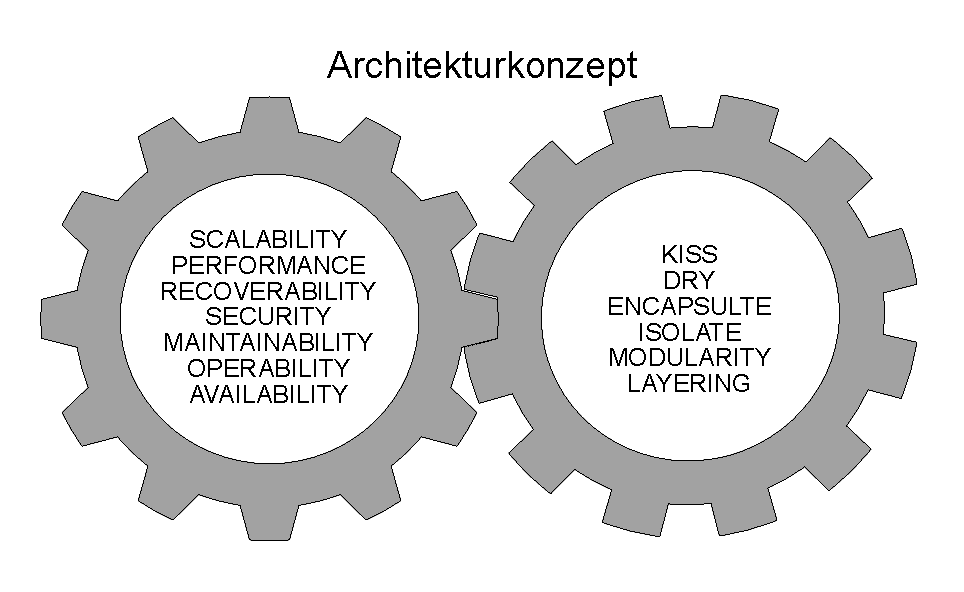
\includegraphics[width=\pictureWidth cm]{Bilder/Sonstiges/Anforderungen_Prinzipien.pdf}
\caption{Allgemeine Prinzipien einer Architektur\label{fig:prinzip}\protect\footnotemark}
\end{figure}
\footnotetext{Brysiuk, Lehmann (2019)}

Die nicht-funktionalen Anforderungen sind im allgemeinen selbsterklärend, deshalb wird nicht weiter auf sie eingegangen. Jedoch bestehen die Prinzipien des Softwareentwurfs aus weniger selbsterklärenden Begriffen und Akronymen, weshalb diese im folgenden genauer erläutert werden.

\subsection*{KISS - Keep it Simple and Stupid}

Bereits im 20. Jahrhundert hat der amerikanische Flugzeugkonstrukteur Clarence Leonard (Kelly) Johnson das \ac{KISS}-Prinzip erstmals erwähnt und treffend beschrieben:
\begin{quote}
\glqq{}Reduce reports and other paperwork to a minimum.\grqq{} \autocite[][231]{biography}
\end{quote}

Die Idee dahinter ist, dass die Gestaltung der Maßnahmen oder Entscheidungen so wenig wie möglich Komplexität beinhalten, jedoch sollen die Ergebnisse die erwarteten Anforderungen erfüllen und dazu flexibel genug sein, um Änderungen vorzunehmen. Also soll die Umsetzung einfach, schnell, verständlich, logisch, begreifbar und passend an die Anforderungen und nicht auf die Möglichkeiten sein. Bei einer Softwarearchitektur darf bei der Einhaltung des \ac{KISS}-Prinzips nicht auf die angemessene Modularisierung verzichtet werden\autocite[Vgl.][19]{gmodse}.

Häufig wird beim Konzeptionieren versucht von Anfang an auf alle möglichen Variationen der Anforderungen einzugehen. Dies umfasst auch die Anforderungen, die noch nicht gestellt wurden, von denen man allerdings ausgeht, as sie im Verlauf des Projektes noch vom Auftraggeber ergänzt werden. Das Ziel davon ist es, in der Zukunft den zusätzlichen Aufwand für die Implementierung zu sparen. Das Problem dabei ist, dass die Wahrscheinlichkeit ziemlich gering ist, dass solche zusätzliche Funktionalitäten tatsächlich noch benötigt werden. Das führt letztendlich zu einer komplexeren Anwendung, deren Flexibilität auf ein Minimum reduziert wird. Dies wird zusätzlich dadurch unterstützt, dass eine Anforderung sich während des Entwicklungsprozesses ändert, da der Auftraggeber oft nicht mehr zufrieden mit der ursprünglichen Lösung ist\footnote{a.a.O., S. 19 f.}.
\\
\linebreak

\begingroup

Folgende Formel zur Berechnung des Nutzen eines Mehrwerts ~$N_{mehrwert}$ kann dazu dienen, besser abschätzen zu können, ob ein gewünschter Mehrwert tatsächlich vorher berücksichtigt werden soll\footnote{a.a.O., S. 20.}:
\\
\linebreak

\begin{dmath}
N_{mehrwert} = (A_{nach} * P_{gebrauch}) - A_{vor}
\end{dmath}

\par
\begingroup
\leftskip=2cm
\rightskip=2cm
\noindent \textit{wobei \\~$A_{vor} =$ Aufwand eines Features bei der Planung von Anfang an\\~$A_{nach} =$ Aufwand eines Features bei späterer Aufnahme\\~$P_{gebrauch} =$ Wahrscheinlichkeit, dass ein Feature später benötigt wird}
\par
\endgroup
\endgroup

\subsection*{DRY - Dont't Repeat Yourself}

<Durch generische Programmierung können Code-Duplikate vermieden werden und wiederholende Algorithmen an mehreren Stellen wiederverwendet werden. Die Idee ist es also beim DRY-Prinzip, die Redundanzen von Programmstellen zu reduzieren , beziehungsweise sie komplett zu vermeiden. Hier ist aber Vorsicht geboten, denn die nicht-funktionalen Anforderungen wie Verfügbarkeit oder Wartbarkeit haben eine höhere Priorität. Man soll alle Prinzipien und Anforderungen auswerten und sogar priorisieren, um eine ausgewogenen Softwarearchitektur erstellen zu können\autocite[Vgl.][21]{gmodse}.

\subsection*{Encapsulation - Prinzip der Kapselung}
Das Konzept des \textit{Information Hidings} wurde bereits im Jahr 1972 von David Parnas vorgestellt:

\begin{quote}
\glqq{}The second decomposition was made using \grqq{}information hiding\grqq{} as a criterion. The modules no
longer correspond to steps in the processing. The line
storage module, for example, is used in almost every
action by the system. Alphabetization may or may not
correspond to a phase in the processing according to
the method used. Similarly, circular shift might, in some
circumstances, not make any table at all but calculate
each character as demanded. Every module in the
second decomposition is characterized by its knowledge
of a design decision which it hides from all others. Its
interface or definition was chosen to reveal as little as
possible about its inner workings.\grqq{} \footcite[][1056]{parmas}
\end{quote}

Der Zweck besteht darin eine Art Geheimnisprinzip zu erstellen, um bestimmte Stellen zu schützen, ob für die Zugriffsberechtigungen oder für die Sicherung der Integrität der Daten. Es werden Komponenten verborgen und eine Schnittstelle für einen öffentlichen Zugriff definiert, somit hat eine Änderung oder der Austausch einer Komponente keine Auswirkung nach außen. Außerdem wird die Robustheit der Anwendung durch die erhöhte Begrenzung der Abhängigkeiten der Komponenten gestärkt\autocite[Vgl.][21\psq]{gmodse}.

\subsection*{Lose Kopplung}
l
\ac{IT}-Systeme bestehen meist aus mehreren Bausteinen, Komponenten und Subsystemen. Diese werden immer zwangsläufig Abhängigkeiten untereinander bilden, da einfach das ganze \ac{IT}-System nicht völlig isoliert werden kann. Die Idee der losen Kopplung ist es, die Verbindungen der einzelnen Bausteine untereinander zu verringern, sowohl auf der Hardware-, als auch auf der Softwareebene. Bei den Verbindungen sollen folgende Punkte berücksichtigt werden\autocite[Vgl.][25\psqq]{gmodse}:

\begin{itemize}
\item Laufzeitumgebungen
\item Ausführungsort
\item Verwendete Technologien
\item Ausführungszeit
\item Daten und Formate bei der Kommunikation
\end{itemize}

\subsection*{Separation Of Concerns}

Auf das Prinzip \textit{Seperation Of Concerns}, zu Deutsch etwa \textit{Trennung der Angelegenheiten}, wurde im Verlauf den gesamten Kapitels immer wieder aufmerksam gemacht und auf dessen Wichtigkeit hingewiesen. \textit{Separation of Concerns} ist das Prinzip der Modularität, welches bereits ausführlich am Anfang des Kapitels \ref{sec:softwarearchitektur} beschrieben wurde.

\subsection*{Layering - Schichtenarchitektur\label{sec:layering}}
Wie bereits in Prinzip der Modularität beschrieben wurde, ist es wichtig beim Entwurf eines \ac{IT}-Systems dieses in einzelne Komponente und Module zu zerlegen. Dabei bilden die Komponenten in ihrem Zusammenspiel auf einer Ebene verschiedene Schichten. Dieser Schichten sind nach Funktionalität getrennt. Beispielhaft ist das in der Abbildung \ref{fig:schichten} dargestellt. Das System besteht aus vier verschiedenen Schichten die wiederum einzelne Komponenten enthalten\footnote{Vgl. a.a.0., S. 31 ff.}.

\begin{figure}[H]
\centering
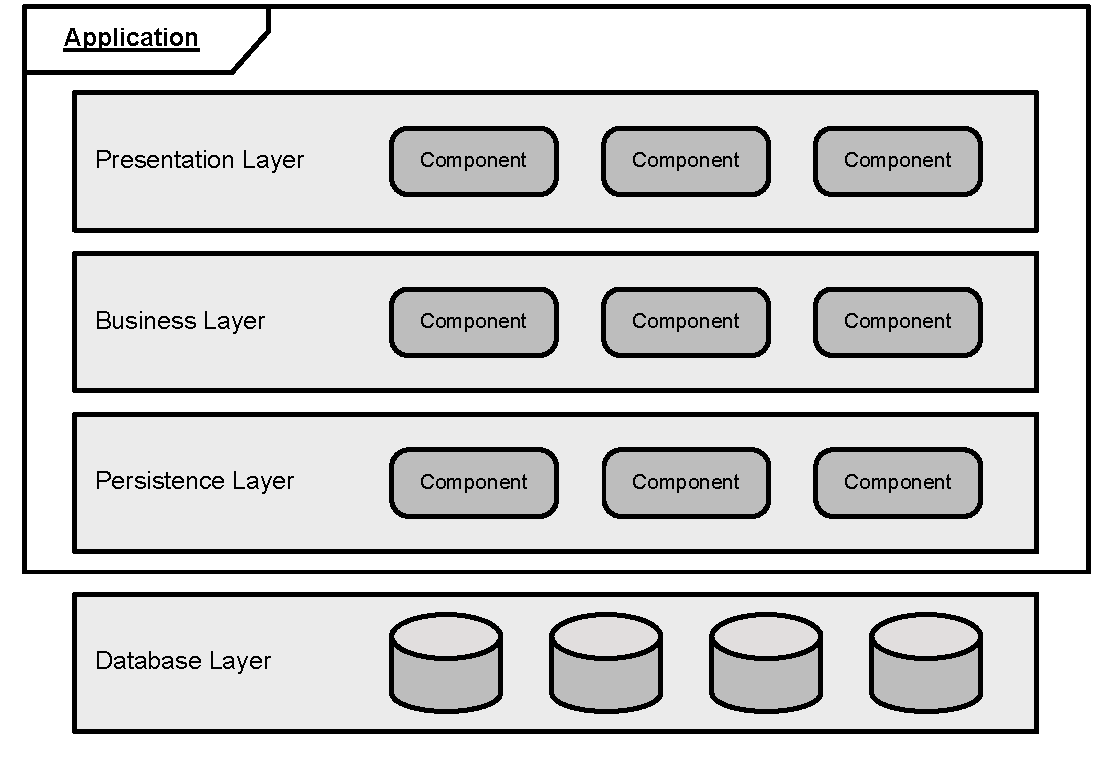
\includegraphics[width=\pictureWidth cm]{Bilder/Architektur/Schichtenarchitektur.pdf}
\caption{Schichtenarchitektur\label{fig:schichten}\protect\footnotemark}
\end{figure}
\footnotetext{Vgl. Dowalil(2018), S. 31 ff.}

Für Entwickler werden große Projekte durch die Einhaltung des \textit{Layerings} deutlich beherrschbarer. Ähnlich wie unser Gehirn solche Zusammenhalte verarbeitet wird das große Ganze in Schichten unterteilt, die sich in Funktionalitäten trennen. Die einzelnen Schichten werden dann wieder in Komponenten zerlegt, bis eine Komponente klein genug ist um sie detailliert zu verstehen. So muss man sich am Ende nur einen Überblick über das Gesamtbild verschaffen\footnote{Vgl. a.a.O., S. 36.}.

\section{Fazit\label{sec:archfazit}}
Die Verbreitung der verteilten Programme, im Englischen \textit{Distributed \acp{App}}, hat sich in den vergangenen Jahren schnell weiterentwickelt. Diese Anwendungen laufen nicht auf einem einzelnen lokalen Rechner, sondern werden auf mehrere unabhängige Module verteilt, die wiederum auf mehreren unterschiedlichen Servern im Netzwerk verteilt sein können. Somit stellen verteilte Anwendungen eine Art verteiltes - beziehungsweise vernetztes - System dar\autocite[Vgl.][3\psq]{verteiltesys}. 
\\
\linebreak
Ein Beispiel hierfür sind Cloud Computing Systeme, diese bauen auf der Softwarearchitektur von verteilten Systemen auf. In Abbildung \ref{fig:cloud_statistic} ist eine Statistik abgebildet, in der das Wachstum für die Nutzung von Cloud Computing Systemen in deutschen Unternehmen in den Jahren 2011 bis 2018 zu sehen. Man erkennt, dass bereits im Jahr 2018 73\% der befragten Unternehmen Cloud Computing Systeme benutzten. Weitere 19\% überlegten oder planten bereits solche Systeme zu nutzen\autocite{cloudstatista}.

\begin{figure}[H]
\centering
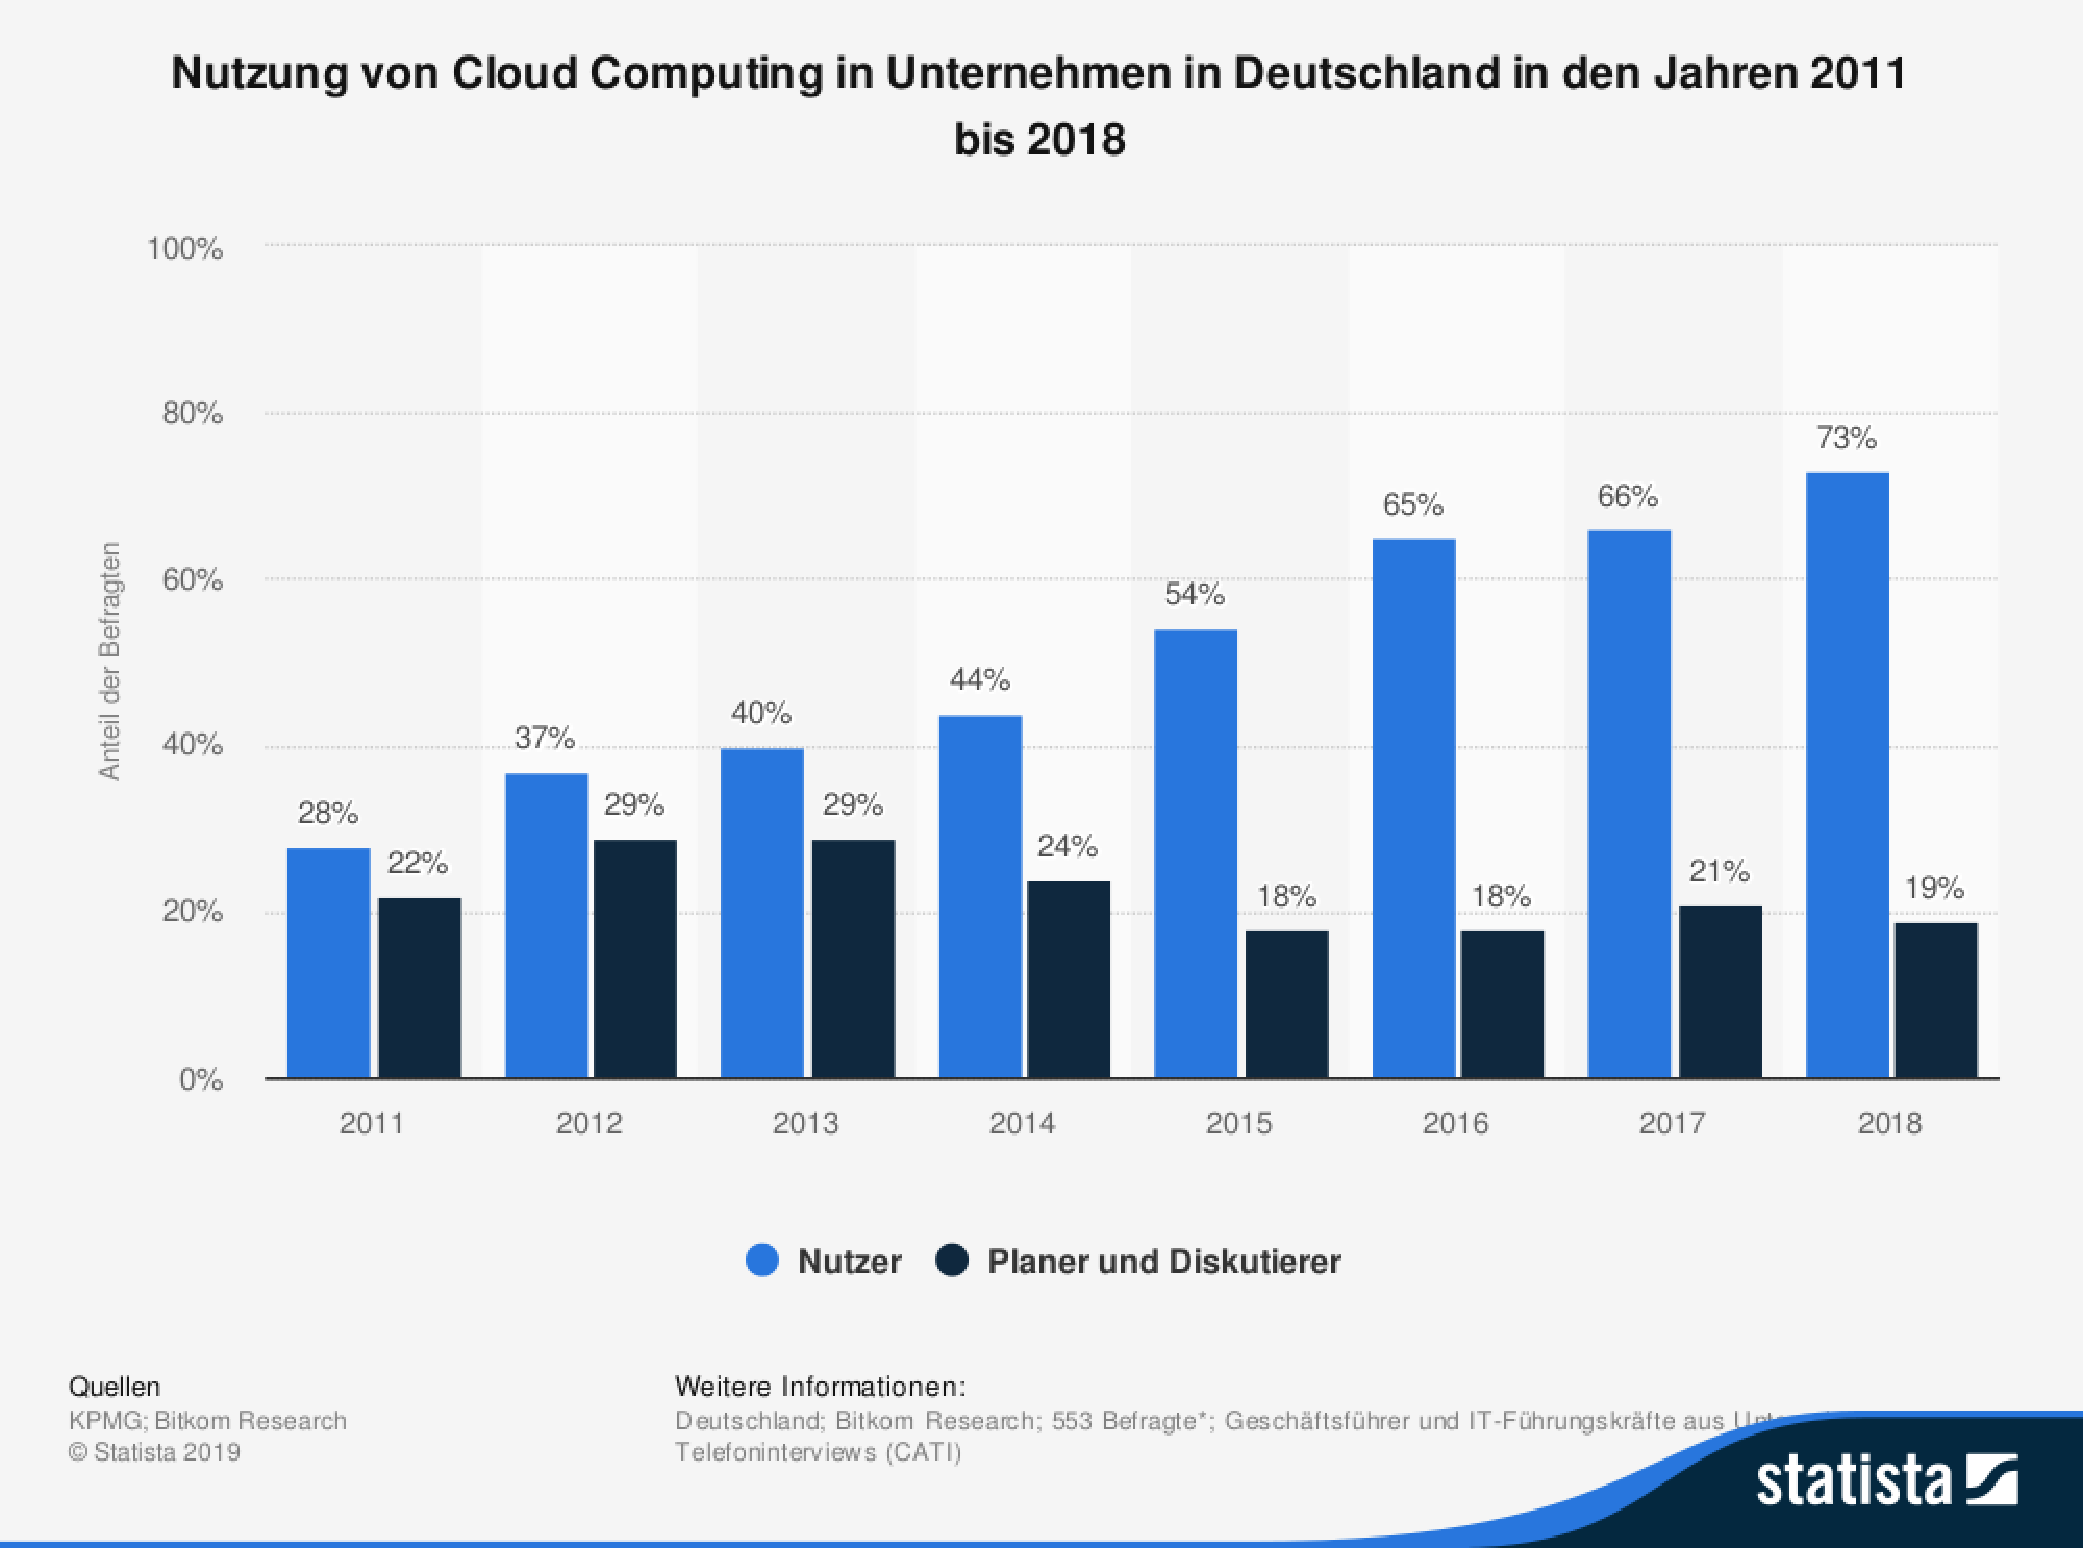
\includegraphics[width=\pictureWidth cm]{Bilder/Statistik/Statista_Cloud_Computing.pdf}
\caption{Nutzung von Cloud Computing\label{fig:cloud_statistic}\protect\footnotemark}
\end{figure}
\footnotetext{ebd.}
% Bitkom, Nutzung von Cloud Computing in Unternehmen in Deutschland in den Jahren 2011 bis 2018 Statista, https://de.statista.com/statistik/daten/studie/177484/umfrage/einsatz-von-cloud-computing-in-deutschen-unternehmen-2011/ (letzter Besuch 14. August 2019)

Wie bereits erwähnt setzen sich verteilte Systeme aus mehreren unabhängigen Modulen zusammen, die auf unterschiedlichen Servern implementiert sind. Durch die Kopplung der Module entsteht ein vollständiges System, welches eine räumliche Trennung über weite geografische Distanzen ermöglicht. Dies ermöglicht einen parallelen und effizienten Zugriff, in unserem Fall zum Beispiel auf Stundenplan- und Mensadaten, denn die Abfragen würden von zwei unterschiedlichen Modulen auf verschiedenen Servern bearbeitet werden. Einen weiterer Vorteil bei dieser Herangehensweise ist der Lastausgleich. Durch eine Modularisierung der Funktionalitäten und der Verteilung dieser auf mehreren Servern, kann die Verarbeitungslast eines zentralen Servers auf mehrere Instanzen verteilt werden, um eine einseitige Auslastungen zu vermeiden. Außerdem wird ein hohes Maß an Fehlertoleranz, Ausfallsicherheit, Skalierbarkeit und Verfügbarkeit auf der Basis verteilter Systeme gewährleistet\autocite[Vgl.][5\psq]{verteiltesys}.

Ausgehend von den bisherig beschriebenen Anforderungen und Prinzipien an die Softwarearchitektur, sowie der Wichtigkeit von Modularisierung und den Anforderungen aus Kapitel \ref{sec:anforderung}, bieten verteilte Systeme eine gute Voraussetzungen für die Architekturkonzepte der Hochschul-\ac{App}. Dabei bieten diese in sich verschiedene Umsetzungen der Systemarchitektur, die teilweise aufeinander aufbauen\footcite[Vgl.][13\psq]{verteiltesys}:
\begin{itemize}
\item Client-Server-Modell
\item Objektorientiertes Modell
\item Komponenten basiertes Modell
\item Dienst orientiertes Modell
\end{itemize}
Verteilte Anwendungen basieren meist auf dem Dienst orientierten Modell, welches auch unter dem Begriff der \textit{Service-orientierten} Architektur im Zusammenhang mit Webservices bekannt ist\footnote{ebd.}.
Somit sind Webservices ein guter Ansatz für die konkrete Implementierung der verteilten Anwendung und der Grundbaustein für die Hochschul-\ac{App}.


% Webservices
\chapter{Web Services}
\label{sec:webservices}

Web Services ermöglichen es, verschiedene Programme miteinander in einem Netzwerk zu verbinden. Hierfür stellen sie eine einheitliche Schnittstelle für die Kommunikation untereinander zur Verfügung. Dabei spielt die Wahl der Plattform - ob Windows, Linux oder \ac{iOS} - als auch die Wahl der Programmiersprachen wie Java, \ac{PHP} oder Python keine Rolle. Somit können einzelne Programme, Module oder Komponenten in unterschiedlichen Sprachen von unterschiedlichen Teams entworfen werden, so wie auf beliebigen Systemen installiert werden. 
\\
\linebreak
Eine der zentralen Funktionen eines Webservices ist die Synchronisation von Client und Server. Ein Webservice stellt dem Client Informationen, zum Beispiel über Datentypen, möglichen Operationen sowie die Parameter und Rückgabewerte und Hinweise darüber, wie diese Aufgerufen werden können, zur Verfügung. Für die Kommunikation ist es wichtig ein Transportprotokoll und das Format für die übertragenen Daten festzulegen. Als Transportprotokolle können beispielsweise \ac{SMTP}, \ac{TCP}, \ac{JMS}, \ac{HTTP} oder \ac{HTTPS} genutzt werden. Übliche Datenformate sind dabei \ac{XML} oder \ac{JSON}. 
\\
\linebreak
Allein mit dem Konzept der Webservices ist die Implementierung einer verteilten Anwendung jedoch nicht möglich. Denn Webservices stellen hauptsächlich Dienste und Funktionen über definierte Schnittstellen und Standards über das Netzwerk zur Verfügung, sie dienen also eher zur Kommunikation der Systeme untereinander und weniger zur Abarbeitung logischer Konzepte. Zudem bieten Webservices kein ausreichendes Maß an loser Kopplung. Wie bereits in Kapitel \ref{sec:archfazit} erwähnt wurde, werden Webservices oft im Zusammenhang mit \ac{SOA} gebracht. Dies liegt daran, dass die grundlegenden Konzepte von \ac{SOA} durch Webservices umgesetzt werden können\autocites[Vgl.][23\psqq]{jws}[Vgl.][8\psqq]{soamws}.

\section{Serviceorientierte Architektur}
\label{sec:ws_soa}

Um zu verstehen, was \ac{SOA} ausmacht und wie es verstanden werden muss empfiehlt es sich folgende Aussage zu lesen:

\begin{quote}
\glqq{}Service Oriented Architecture (SOA) is an architectural paradigm that has gained significant attention within the information technology (IT) and business communities.\grqq{} \autocite[][]{oasisspec}
\end{quote}

Eine konkrete oder einheitliche Definition für \ac{SOA} existiert derzeit nicht, deswegen wird \ac{SOA} als ein Paradigma der Architektur bezeichnet. Außerdem ist \ac{SOA} eben deswegen nicht wirklich eine Architektur, sondern eher ein Design/Konzept für verteilte Systeme. Da viele unter \ac{SOA} etwas unterschiedliches verstehen und das Paradigma meistens verschieden implementiert wird, hat die \ac{OASIS} ein \ac{SOA}-Referenzmodell definiert um es zu vereinheitlichen\autocites[Vgl.][11]{soamws}[Vgl.][2\psq]{soaidp}[Vgl.][]{oasis}.

\begin{figure}[H]
\centering
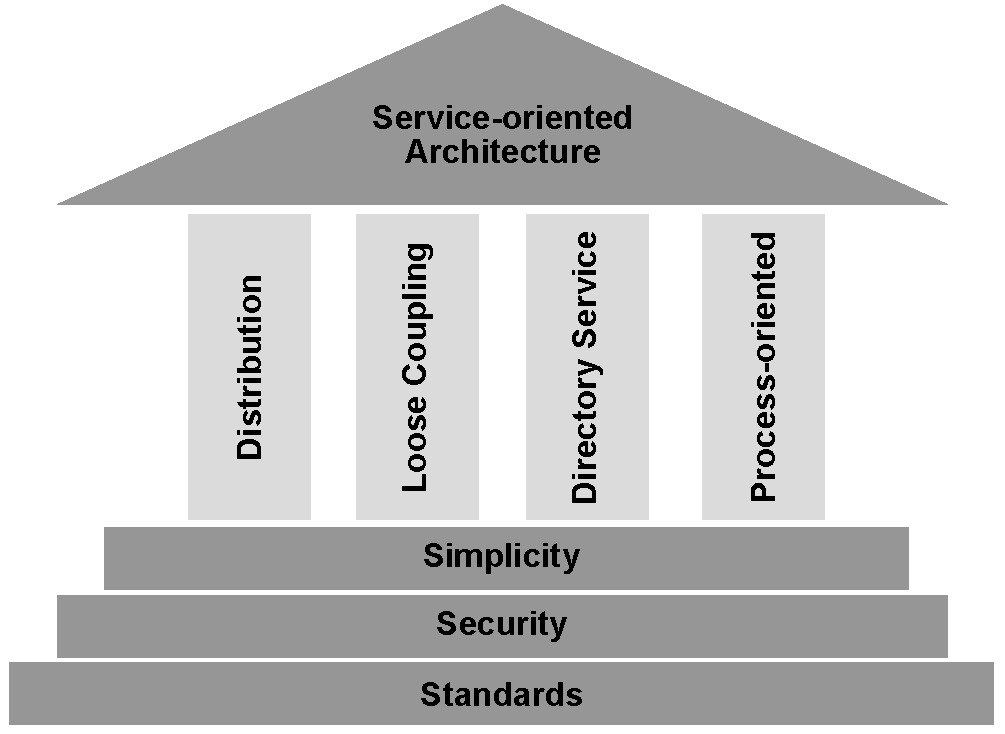
\includegraphics[width=\pictureWidth cm]{Bilder/Sonstiges/SOA_Tempel_Melzer.pdf}
\caption{SOA Tempel\label{fig:soatempel}\protect\footnotemark}%autocite[][11\psq]{soamws}}
\end{figure}
\begin{quote}
\footnotetext{Melzer (2007)}

Autor Ingo Melzer beschreibt das Grundkonzept von \ac{SOA} passend als einen Tempel, wie er in Abbildung \ref{fig:soatempel} zusehen ist, über den er folgendes sagt:

 \glqq{}Das Fundament wird von offenen Standards, Sicherheit und Zuverlässigkeit gebildet. Die verteilten Dienste, die lose Kopplung, die Plattformunabhängigkeit und die prozessorientierte Struktur sind die tragenden Säulen.\grqq{} \footnote{a.a.O., S. 11 f.}
\end{quote}

Aus diesen grundlegenden Aussagen über \ac{SOA} können einige Schlussfolgerungen abgeleitet werden. Durch das Paradigma \ac{SOA} wird die funktionale Zerlegung eines Gesamtsystems in einzelne Komponenten, genannt Services, und die Verteilung dieser auf ein Netzwerk ermöglicht. Wobei hierfür die einzelnen Services Plattform-, sprachen- und Frameworkunabhängig von einander entwickelt und wiederverwendet werden können\autocite[Vgl.][121\psq]{gmodse}.

\subsection{Technische Konzepte}
Um das Potential von \ac{SOA} nutzen zu können, werden verschiedene technische Konzepte verwendet. Die wichtigsten technischen Konzepte von \ac{SOA} sind folgende\autocite[Vgl.][11]{soaidp}:

\begin{itemize}
\item \subsubsection*{Interoperabilität} Unter Interoperabilität ist die Sicherstellung der Kommunikation unterschiedlichen Systemen ohne großen Aufwand miteinander gemeint - mit den Fokus auf den Datenfluss.
\item \subsubsection*{Services} Services dürfen nicht mit Webservices verwechselt werden. Webservices sind ein technisches Konzept zur Umsetzung der Kommunikation in \ac{SOA}, wobei Services in \ac{SOA} funktionale Komponenten sind\autocite[Vgl.][123\psq]{gmodse}.
\item \subsubsection*{Lose Kopplung} Wurde bereits in Unterkapitel \ref{sec:prinzipien} ausführlich behandelt.
\end{itemize}

\subsection{Zusammenfassung}
\label{ws:zf}
Die Service orientierte Architektur mit Unterstützung von Web Services bietet eine gute Voraussetzung für die Abdeckung der nicht-funktionalen Anforderungen sowie der Prinzipien für eine Softwarearchitektur aus Kapitel \ref{sec:architektur}. An folgender Stelle wird genauer erläutert, welche nicht-funktionalen Anforderungen vorhanden sind und warum diese von \ac{SOA} in Kombination mit Webservice-Ansätzen erfüllt werden:

\begin{itemize}
\item \subsubsection*{Skalierbarkeit} 
Durch die Implementierung der Anwendung als verteiltes System kann diese auf einen beliebigen Server mit den benötigten Ressourcen ausgelagert werden. Sollten die Ressourcen irgendwann unvorhergesehen nicht mehr ausreichen, kann die Anwendung auf einen anderen Server ausgelagert werden, ohne eine Beeinflussung der Funktionalitäten der Anwendung zu erzwingen. Eine weitere Möglichkeit hierfür ist die Auslagerung der Anwendung in eine Cloud, diese Vorgehensweise ist auch als \ac{IaaS} bekannt. Unter \acp{IaaS} sind Cloud-Computing-Plattformen gemeint, die Speicher und Rechenleistung auf den Servern für die Benutzer zur Verfügung stellen. Einer der bekanntesten \acp{IaaS} ist der \ac{AWS}. Durch die Auslagerung der Anwendung auf die \ac{AWS}-Cloud wird das Management Werkzeug \textit{Elastic Beanstalk} für den Benutzer zur Verfügung gestellt. Das Elastic Beanstalk übernimmt automatisch das Management über die Bereitstellung zusätzlicher Kapazitäten, Lastenverteilung sowie die Skalierung\autocite[Vgl.][]{aws}.
\\
\linebreak
%AWS https://docs.aws.amazon.com/de_de/elasticbeanstalk/latest/dg/Welcome.html
Eine weitere Möglichkeit dafür, die Skalierbarkeit zu erhöhen, bieten Docker Container. Die Anwendung kann ebenso wie auf mehrere Server auch in einen Docker Container verschoben werden. Die Container lassen sich leicht von einem System auf ein anderes übertragen, benötigen weniger Ressourcen als virtuelle Maschinen und sollten zusätzliche Instanzen der Anwendung benötigt werden, dann können einfach neue Container gestartet werden. Sobald diese nicht mehr benötigt werden, können diese ebenso wieder gestoppt werden\autocite[Vgl.][]{docker}. Somit steht der Skalierbarkeit der Anwendung nichts im Wege.

\item \subsubsection*{Performance} 
Generell gilt, dass die Ladezeiten einer Anwendung in der Regel nicht länger als Drei Sekunden dauern dürfen. Die Performance von \ac{SOA} hängt zunächst von unterschiedlichen Faktoren ab. Manche können eher gut beeinflusst und optimiert werden, andere eher weniger. Die heutige Technologie ist ausreichend ausgereift für die Implementierung schneller und effizienter verteilter Anwendungen. Ein Beispiel dafür ist der weltbekannte Streaming-Anbieter Netflix, der bereits die erwähnten \acp{IaaS} von \ac{AWS} verwendet. Die Filme oder Serien lassen sich in Echtzeit in beliebiger Auflösung streamen\autocite[Vgl.][]{netflix}.
%https://aws.amazon.com/de/solutions/case-studies/netflix/
Außerdem ermöglicht \ac{SOA} bei einem unerwartet hohen Zugriff immer noch das Management der Lastenverteilung der einzelnen Komponenten. Somit wird die Performance durch höhere Auslastungen der Anwendung nicht beeinflusst.

\item \subsubsection*{Verfügbarkeit} 
Eine Anwendung soll im Idealfall permanent erreichbar sein. Ein hohes Maß an Verfügbarkeit kann durch \ac{SOA} erbracht werden. Durch die Replikation der Anwendung auf mehreren Servern, als \ac{IaaS} oder durch Auslagerung in den Docker-Container, kann bei einem Ausfall einer Instanz eine andere Instanz verwendet werden.

\item \subsubsection*{Sicherheit} 
Sicherheit ist einer der Wichtigsten Aspekten in einer Software, denn auch für die Anwendungen, die keine vertraulichen Informationen beinhalten, sollte immer einer Sicherheitskonzept entworfen werden. Bei einer Absicherung eines Webservices spielen folgende Aspekte eine wichtige Rolle:
\begin{itemize}
\item Authentifizierung
\item Autorisierung
\item Integrität
\end{itemize}
Es ist nicht unmöglich eine sichere Service-orientierte Architektur zu konzipieren, dennoch muss dafür frühzeitig auf die Sicherheitsaspekte eingegangen werden. Zu diesen Themen existieren bereits eine Reihe bewährter Technologien, Techniken und Standards um Webservices sicherer zu gestalten\autocite[Vgl.][188\psq]{soamws}.
\\
\linebreak
Um die Vertraulichkeit im Nachrichtenaustausch aufbauen zu können, können verschiedene Methoden des symmetrischen oder asymmetrischen Verschlüsselungsverfahren verwendet werden. Außerdem sind folgende Standards in Webservices bereits etabliert und erleichtern die Implementierung der Sicherheitsaspekte enorm:\footnote{Vgl. a.a.O., S. 190 f.; Vgl. a.a.O., S. 208 ff.}
\begin{itemize}
\item WS-Security
\item WS-Policy
\item WS-Trust
\item WS-SecureConversation
\item WS-Privacy
\item WS-Federation
\item WS-Authorization
\end{itemize}
Wie die Authentifizierung, Autorisierung und Vertraulichkeit in einem Web\-service gewährleistet werden kann, wird ausführlicher in der Bachelorarbeit zur Planung der Nutzerverwaltung und des Frontends der Stundenplan-\ac{App} der Hochschule Hof behandelt\autocite[Vgl.][]{andreasba}. 

\item \subsubsection*{Wartbarkeit} 
Die Wartbarkeit ist einer der Wichtigsten nicht-funktionalen Anforderungen, denn in der Praxis ist es oft der Fall, dass die Anforderungen an die Anwendungen sich mit der Zeit ändern oder neue Funktionalitäten hinzu kommen. Außerdem werden des öfteren erst nach einiger Zeit Fehler in der Anwendungen erkannt, die während der Entwicklung verborgen geblieben sind. Durch die modulare und flexible Gestaltung der Services in einer \ac{SOA} sind diese leicht Austausch- oder Änderbar.
\end{itemize}

Im weiteren Verlauf wird nun erläutert, welche Prinzipien der Softwarearchitektur durch \ac{SOA} in Verbindung mit Webservice-Ansätzen bereits von Beginn an gegeben sind.

\begin{itemize}
\item \subsubsection*{Kapselung} 
Services stellen eine definierte Schnittstelle für den Zugriff bereit, jedoch sind die genauen Details der Implementierung für den Benutzer unsichtbar\autocite[Vgl.][13]{soamws}.
\item \subsubsection*{Lose Kopplung} 
Die Services können auf verschiedenen Systemen in verschiedenen Programmiersprachen realisiert werden, dadurch wird die Kopplung zwischen den Hardware- und Softwareebenen verringert.
\item \subsubsection*{Modularisierung} 
Durch die Trennung der logischen Funktionalitäten in einzelne Komponenten und der Verteilung dieser auf verschiedene Services werden die Abhängigkeiten der Komponenten reduziert. Außerdem entsteht eine fachliche Trennung der Funktionalitäten. 
\item \subsubsection*{Layering} Die Umsetzung von Service-orientierten Architekturen kann in mehreren \\Schichten realisiert werden, die bereits in Abbildung \ref{fig:schichten} zu sehen waren und im Kapitel \ref{sec:schichtenarchitektur} detaillierter beschrieben werden.
\end{itemize}

Somit bietet die Service-orientierte Architektur mit Webservices einen idealen Ansatz für die Umsetzung einer sicheren und zukunftsfähigen Hochschul-\ac{App}. Jedoch kann die Realisierung von Webservices nochmals durch zwei Arten unterschieden werden, \ac{SOAP} und \ac{REST}.


\section{Webservice Arten}
In den weiteren Unterkapiteln werden die beiden Webservice Arten kurz erklärt und anhand einer Entscheidungsmatrix gegenübergestellt und bewertet. Zu unterscheiden ist, dass \ac{SOAP} ein definiertes Netzwerkprotokoll ist, das auf \ac{XML} basiert. \ac{REST} ist hingegen ein \textit{Webservice-Light-Technologie} Architekturstil, der sich nur auf das Kommunikationsprotokoll \ac{HTTP}, respektive \ac{HTTPS}, beschränkt und meisten mit dem \ac{JSON}-Datenformat in Verbindung gebracht wird\autocite[Vgl.][23\psqq]{jws}.

\subsection{Simple Object Access Protocol (SOAP)}

\begin{quote}
\glqq{}[Simple Object Access Protocol] provides a simple and lightweight mechanism for exchanging structured and typed information between peers in a decentralized, distributed environment using XML.\grqq{} \autocite[][]{w3soa}
%https://www.w3.org/TR/2000/NOTE-SOAP-20000508/
\end{quote}
\ac{SOAP} wurde durch das \ac{W3C} als industrieller Standard definiert, in dem es in drei wesentlichen Teile aufgeteilt ist:
\begin{itemize}
\item \subsubsection*{SOAP Envelope} 
Der \ac{SOAP}-Envelope definiert ein Framework, das beschreibt, was in einer Nachricht enthalten ist, wer damit umgehen sollte, und ob gewisse Parameter optional oder obligatorisch sind. Die \ac{SOAP} Nachricht besteht aus einem Envelope, einem Header und einem Body und ist als \ac{XML}-Dokument realisiert. Es wird dadurch versucht für alle Systeme den gleichen Sprachsatz zu definieren - für Anfragen und Antworten. Somit können Nachrichten mit beliebigem \ac{XML}-Inhalt ausgetauscht werden\autocite[Vgl.][]{w3soa}.
%übersetzt aus https://www.w3.org/TR/2000/NOTE-SOAP-20000508/
Durch die Trennung des Bodies vom Header entsteht eine saubere Trennung zwischen den Anwendungsdaten und Webservice spezifischen Daten\autocite[Vgl.][63\psq]{jws}

\item \subsubsection*{SOAP Encoding Regeln} 
Diese Regeln definieren einen Serialisierungsmechanismus, mit dem anwendungsdefinierte Datentypen zwischen den Services ausgetauscht werden können. Wobei hier anzumerken ist, dass \ac{XML} eine sehr flexible Codierung von Daten ermöglicht. Die unter dem \ac{W3C} beschriebenen Kodierungsregeln können in Verbindung mit der \ac{RPC}-Darstellung verwendet werden\autocite[Vgl.][]{w3soa}.
%übersetzt aus https://www.w3.org/TR/2000/NOTE-SOAP-20000508/

\item \subsubsection*{SOAP RPC-Darstellung} 
Eines der Entwurfsziele von \ac{SOAP} besteht darin, \ac{RPC}-Aufrufe unter Verwendungen der Erweiterbarkeit und Flexibilität von \ac{XML} zu kapseln und auszutauschen\footnote{ebd.}.
%übersetzt aus https://www.w3.org/TR/2000/NOTE-SOAP-20000508/
Bei der Verwendung von \ac{SOAP} durch \acp{RPC} sind folgende Transportprotokollbindungen möglich\autocite[Vgl.][85\psq]{soamws}:
\begin{itemize}
\item \ac{TCP}
\item \ac{HTTPS}
\item \ac{SMTP}
\item \ac{FTP}
\item \ac{JMS}
\item \ac{RMI}
\end{itemize}

\end{itemize}

Ein weiterer industrieller Standard des \ac{W3C} ist die \ac{WSDL}. Diese stellt ein Model und ein \ac{XML}-Format zur Beschreibung der Webservices bereit. Zusammen mit \ac{SOAP} entsteht eine Grundlage für Webservice Anwendungen\footnote{Vgl. a.a.O., S. 101 f.}.
Jedoch hat die Realität gezeigt, dass \ac{SOAP} weder leicht in der Umsetzung ist, noch tatsächlichen Zugriff auf die Objekte bietet, es ist somit eher ein Kommunikationsprotokoll für Webservice Anwendungen. Durch die Bindung von unterschiedlichen Transportprotokollen, können unterschiedliche Arten von verteilten Anwendungen mit Hilfe von \ac{SOAP} entwickelt werden. Das Problem bei \ac{SOAP} besteht darin, dass eine \ac{SOAP} Nachricht mit dem \ac{XML}-Datenformat unnötig viel Overhead produziert. Für einen einfachen, beispielhaften Request an die Hochschul-\ac{App}, wie \lstinline[columns=fixed]{getAllLectures},%[ 
die keine Parameter und keinen Body enthalten, muss dennoch ein Body definiert werden. Bei einem kleinen Datendurchsatz stellt dies noch keine Probleme dar, jedoch wird es mit Steigerung der Daten problematisch, kompliziert und ineffizient\autocite[Vgl][57\psq]{jws}.
\\
\linebreak
Aus diesem Grund wurde im Jahr 2000 durch Roy Thomas Fielding ein vereinfachter Architekturstil namens \ac{REST} eingeführt, der, wie bereits am Anfang des Kapitel erwähnt wurde, auf das \ac{JSON}-Datenformat und das Kommunikationsprotokoll \ac{HTTPS} basiert\autocite[Vgl][77\psq]{jws}.

\subsection{Representational State Transfer (REST)}
\ac{REST} hat seinen Ursprung bereits vor den Webservices, denn es wurde damals versucht die jetzt unter \ac{REST} bekannten Prinzipien als Architekturleitpfad für das Internet zu verwenden. Durch Roy Thomas Fielding wurde \ac{REST} mit Webservices kombiniert und damit eine neue Revolution von der Prinzipien ausgelöst. Von nun an war \ac{REST} auch unter dem Namen RESTful Webservice oder RESTful Web-\ac{API} bekannt. Die Webseite \textit{www.programmableweb.com} bietet eines der größten Archive für Web-\acp{API} im Internet an. Im Juli 2019 hat die Webseite eine Statistik für den Wachstum des Web-\ac{API} Archivs seit 2005 veröffentlicht\autocite[][]{apiarchive}.

\begin{figure}[H]
\centering
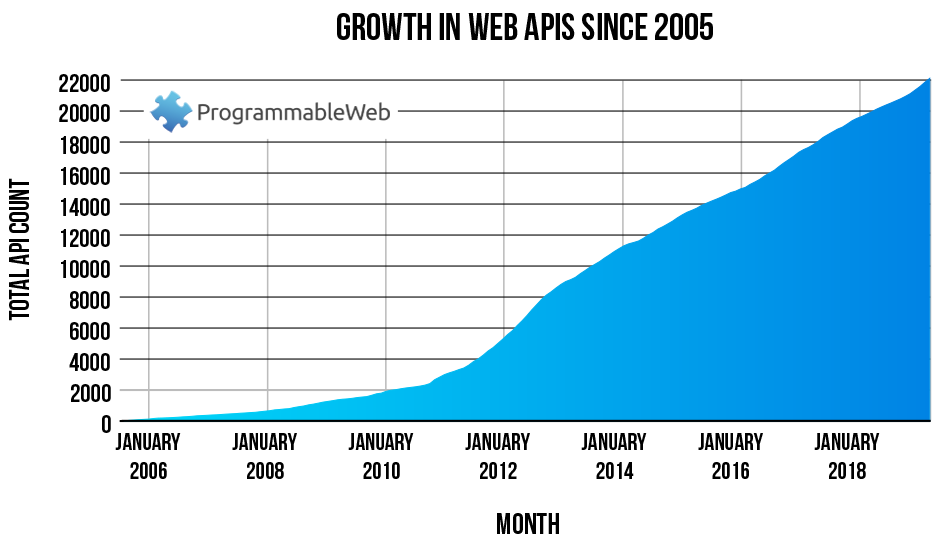
\includegraphics[width=\pictureWidth cm]{Bilder/Statistik/ProgrammableWebApis.png}
\caption{Wachstum der ProgrammableWeb API Archive von 2005\label{fig:api_statistic}\protect\footnotemark}
\end{figure}
\footnotetext{ebd.}
%https://www.programmableweb.com/news/apis-show-faster-growth-rate-2019-previous-years/research/2019/07/17

Anhand der Statistik in Abbildung \ref{fig:api_statistic} ist deutlich zu erkennen, dass die Anzahl von Web-\acp{API} seit 2006 kontinuierlich steigt. Das Potential von \ac{REST} wurde schnell erkannt, obwohl \ac{REST} immer noch - im Gegensatz zu SOAP - kein industrieller Standard, sondern eher eine Richtlinie ist, die die möglichen Nachteile von SOAP umgehen soll. Genauere Ansätze und die erwähnten Richtlinien zu \ac{REST} werden noch im Kapitel \ref{sec:ms} beschrieben.

\subsection{Bewertung}

Die folgende Entscheidungsmatrix \ref{tab:restvssoap} dient dazu, die beiden Webservice Arten gegenüberzustellen und eine Entscheidung darüber zu treffen, welche der Webservice Arten besser für die Hochschul-\ac{App} geeignet ist.

\begin{table}[H]
\begin{center}
  \begin{tabular}{| l | c | c |}
    \hline
    \rowcolor{Gray}
    \textcolor{white}{\textbf{Kriterien}} & \textcolor{white}{\textbf{REST}} & \textcolor{white}{\textbf{SOAP}} \\ \hline
    Unterstützung leichtgewichtiger Clients 		& 1 			& 0 \\
    \hline
\rowcolor{LGray}    
    Geringere Komplexität 						& 1 			& 0 \\
    \hline
    Effizienz			 						& 1 			& 0 \\
    \hline
    \rowcolor{LGray}
    Unterstützung unterschiedlichen Datenformate	& 1 			& 1 \\
    \hline
    Caching-Mechanismen	 						& 1 			& 0 \\
    \hline
    \rowcolor{LGray}
    Industrieller Standardisierung				& 0 			& 1 \\
    \hline
    Unterschiedliche Kommunikationsprotokolle		& 0 			& 1 \\
    \hline
    \rowcolor{LGray}
    Sicherheit			 						& 1 			& 1 \\
    \hline
   	\textbf{Ergebnis}							& \textbf{6}			& \textbf{4} \\
    	\hline
    	
  \end{tabular}
  \end{center}
\caption[Entscheidungsmatrix SOAP und REST]{Entscheidungsmatrix}
\label{tab:restvssoap}
\end{table}

Bedeutung der Bewertungszahlen: 
\begin{itemize}
\item \textbf{1:} trifft zu
\item \textbf{0:} trifft nicht zu
\end{itemize} 

\ac{REST} schneidet mit 2 Punkten besser als \ac{SOAP} ab. Aus diesem Grund und vor allem, da \ac{REST} für leichtgewichtige Clients wie Browser oder Smartphones entwickelt wurde und auch leichter für diese zu implementieren ist, da der ganze Overhead entfällt und es zahlreiche Caching-Mechanismen unterstützt werden, geht \ac{REST} als Sieger für die Entwicklung der Hochschul-\ac{App} hervor. Somit stellt \ac{REST} eine interessantere Grundlage für das Design der Hochschul-\ac{App} dar.
\\
\linebreak
Um die Entscheidungsmatrix und die aufgeführten Punkte, die für \ac{REST} sprechen, zu verstehen, wird im nächsten Kapitel näher  auf die beschriebenen Merkmale und Richtlinien von \ac{REST} eingegangen.

% REST playbook
\chapter{REST API Design}
\label{sec:ms}
Wie bereits zuvor erwähnt wurde, ist \ac{REST} \ac{API} kein industriell definierter Standard, weswegen es zahlreiche Varianten der Implementierung und Umsetzung gibt. Das Ziel dieses Kapitels ist es, allgemeingültige Richtlinien und Entwurfsstandards für die Erstellung einer \ac{REST}-\ac{API} der Hochschul-\ac{App} festzulegen. Diese Standards helfen beim genaueren Erarbeiten einer \acp{API}, die intuitiv ist und von den Entwicklern leicht verstanden und wieder- oder weiterverwendet werden kann.
\\
\linebreak

Eine \ac{REST}-\ac{API} kann in vier Bereiche aufgeteilt werden:

\begin{enumerate}
\item Ressourcen
\item Requests
\item Responses
\item Hypermedia
\end{enumerate}

Diese Bereiche werden in den kommenden Kapitel ausführlicher behandelt.

\section{Ressourcen Design}

Das folgende Kapitel betrifft Standards und Richtlinien für die Modellierung und Benennung von \ac{URI} Ressourcen, sowie für die Handhabung der HTTP-Methoden.

\subsection{Versionsverwaltung}

Die Versionierung ist ein wichtiger Aspekt des \ac{API}-Designs. Es kann jederzeit nachvollzogen werden, wann und was sich zu einer Version geändert hat - bei einem Problem kann das System auf eine vorherige Version wiederhergestellt werden. Somit soll jede \ac{API} einer Versionsnummer zugeordnet werden. Die Version kann aus einer Hauptversion und optional aus einer Nebenversion bestehen. Hierzu gibt es verschiedene Ansätze für die Versionsverwaltung. Es können bei verschiedenen Methoden, den Request-Parametern oder bei individuellen Headern die gewünschte Version angegeben werden. Zur Vereinfachung sollte das \ac{KISS}-Prinzip aus Kapitel \ref{sec:prinzipien} angewendet werden und die Version im Pfad der \ac{URI} mit dem Präfix \textit{v} und der Hauptversionsnummer angegeben werden. Bei folgenden Änderungen sollte die Version erhöht werden:

\begin{itemize}
\item Pflichtfeld wird als optional abgeändert oder umgekehrt
\item Pflichtfeld oder optionales Feld wird eingefügt
\item Ressourcen werden eingefügt, abgeändert oder entfernt
\item Datentypen werden hinzugefügt, geändert, entfernt oder eingeschränkt
\item Fehlercodes werden ergänzt
\end{itemize}

\subsection{URI Namenskonvention}

\ac{API}-\acp{URL} sollten folgende Kriterien enthalten:

\begin{itemize}
\item Adresse des Servers, auf dem die \ac{API} gehostet wird
\item Kennzeichnung, dass es sich um einen \ac{API}-Endpunkt handelt
\item Spezifizierung des \ac{API}-Namens
\item Spezifizierung der Version der \ac{API}
\item Spezifizierung der Ressource
\item Jede Pfadebene der Ressourcen muss sinnvolle Informationen liefern
\end{itemize}

Durch Beachtung dieser Kriterien sollte eine \ac{API}-\ac{URL} folgendermaßen aussehen:

\begin{lstlisting}[caption={URL Namenskonvention}, commentstyle=\color{black},]
http[s]://<server>/api/<api-name>/<api-version>/<resource>
https://hof-university.de/api/mensa-service/v1/menu
\end{lstlisting}

\subsection{Ressourcen Namenskonvention}

Folgende Namenskonventionen sollten für die Ressourcen in der Hochschul-\ac{App}-\ac{API} eingehalten werden:

\begin{itemize}
\item Jede Ressource muss einen aussagekräftigen und selbsterklärenden Namen haben. 
\item Wenn eine Ressource über Subressourcen verfügt, so werden diese durch Schrägstriche getrennt und der Pfad zur Subressourcen sollte hierarchisch und selbsterklärend aufgebaut werden.
\end{itemize}

Dies kann beispielsweise folgendermaßen aussehen:

\begin{lstlisting}[caption={Subressourcen Aufbau}]
/menu
/menu/{day}
/menu/{day}/{category}
\end{lstlisting}

Die Ressource \lstinline[columns=fixed]{/menu} soll %[]

\begin{itemize}

\item  alle verfügbaren Informationen zum \textit{Menü} liefern, 
\lstinline[columns=fixed]{/menu/today} nur für den heutigen Tag und \lstinline[columns=fixed]{/menu/today/desserts} nur für den heutigen Tag und nur für die Desserts,
\item keine \ac{CRUD} Operationsnamen in Ressourcen verwenden,
\item keine Mischung zwischen Groß- und Kleinschreibung enthalten,
\item keine Zeichen, die eine URL-Codierung erfordern, verwenden, 
\item Bindestrich anstelle eines Leerzeichens oder einer Unterstreichung verwenden.
\end{itemize}

\subsection{HTTP Methoden}
Nach der Identifizierung der Ressourcen für eine \ac{API} \footnote{Siehe Kapitel \ref{sec:appservices}}, muss die Aktion, die für diese Ressource ausgeführt werden soll, festgelegt werden. Dafür werden die HTTP-Methoden verwendet um die ausführende Aktion anzugeben. Die primären und am häufigsten verwendete HTTP-Methoden sind POST, GET, PUT und DELETE. 

\begin{figure}[H]
\centering
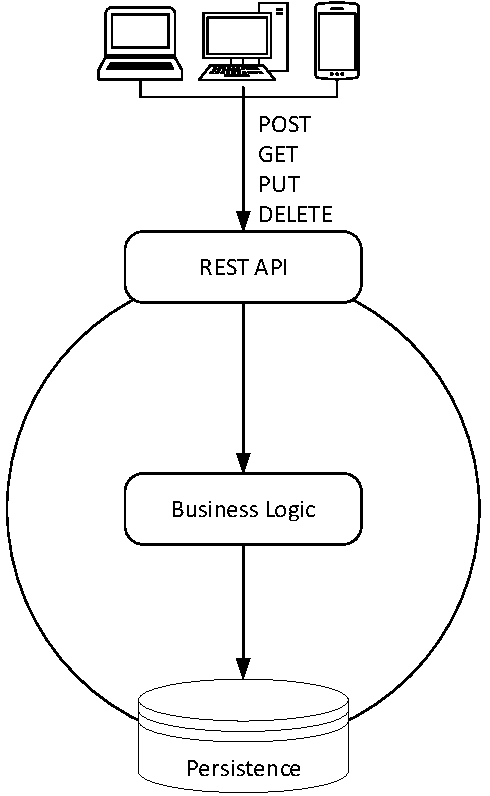
\includegraphics[width=\pictureWidth cm - 7.5 cm]{Bilder/Sonstiges/Rest_Api_HTTP.pdf}
\caption{Einordung der \ac{HTTP}-Methoden in  die Gesamtarchitektur\label{fig:api}\protect\footnotemark}
\end{figure}
\footnotetext{Brysiuk, Lehmann (2019)}


Diese Methode helfen bei der Ausführung der \ac{CRUD}-Operationen für die Ressource. Die Richtlinien für die Verwendung der Methoden in der Hochschul-\ac{App}-\ac{API} werden in Tabelle \ref{tab:httpmethoden} erläutert\autocite[Vgl.][]{httpwiki}.

\begin{table}[H]
\begin{center}
  \begin{tabular}{|  p{0.14\textwidth} |  p{0.8\textwidth} |}
  	\hline
  	\rowcolor{Gray}
  	\textcolor{white}{\textbf{Methoden}}			& \textcolor{white}{\textbf{Definition}} \\
    \hline
    GET		 									& Wird zum Abrufen oder Lesen der Informationen verwendet
    \\ \hline
    \rowcolor{LGray}
    POST									 		& Wird zum Erstellen einer neuen Ressource verwendet
    \\ \hline
    PUT									 		& Wird zum Aktualisieren/Änderung einer ganzen Ressource verwendet
    \\ \hline
    \rowcolor{LGray}
    DELETE								 		& Wird zum Löschen einer vorhandenen Ressource verwendet
    \\ \hline
    PATCH								 		& Wird zum Aktualisieren/Änderung eines teils einer Ressource verwendet
    \\ \hline
    \rowcolor{LGray}
    TRACE										& Wird zur Verfolgung von den Request verwendet
    \\ \hline
    OPTIONS								 		& Anforderung einer Liste vorhandenen HTTP-Methoden für diese Ressource
    \\ \hline
    \rowcolor{LGray}
    HEAD											& Ähnlich wie GET, jedoch wird nur der Response-Header zurückgegeben
    \\ \hline
    CONNECT										& Bereitstellung eines \ac{SSL}-Tunnels von Proxyservern %https://wiki.selfhtml.org/wiki/HTTP/Anfragemethoden
    \\ \hline
  \end{tabular}
  \end{center}
\caption[HTTP-Methoden]{Erläuterung der HTTP-Methoden}
\label{tab:httpmethoden}
\end{table}

Zudem kann die Methode \textit{TRACE} dazu dienen, die Requests auf Veränderungen während der Übertragung dieser zu überprüfen. \textit{HEAD} bietet unter anderem die Möglichkeit, die gecachten Daten auf Ihre Gültigkeit zur prüfen, ohne die ganzen Daten komplett neu anzufordern\autocite[Vgl.][]{httpwiki}.
%https://wiki.selfhtml.org/wiki/HTTP/Anfragemethoden

\section{Request Struktur}
\label{sec:reqstructure}

Das folgende Kapitel behandelt die Nachtrichten-Struktur-Richtlinien für Inhalt, Format, Header und Query Parameter einer Nachricht.

\subsection{Header}

Die folgende Liste enthält HTTP-Header, die von der Hochschul-\ac{App}-\acp{API} verwendet werden sollen:

\begin{itemize}
\item Accept
\item Authorization
\item Content-Type
\item X-HTTP-Method-Override
\end{itemize}

Das Payload-Format der Hochschul-\ac{App} wird nur auf das Format \ac{JSON} beschränkt, da \ac{JSON} einige Vorteile gegenüber anderen Formaten bietet, was in Kapitel \ref{sec:webservices} bereits erwähnt wurde. Mit dem Header \lstinline[columns=fixed]{accept} %[
kann der Medientyp des erwarteten Antwortinhalts und mit dem \lstinline[columns=fixed]{content-type} %[
der Medientyp des Requests angegeben werden. Also wird der \textit{Mediatype} als \lstinline[columns=fixed]{application/json} im \lstinline[columns=fixed]{content-type} und im \lstinline[columns=fixed]{accept} Header definiert. Der Header \lstinline[columns=fixed]{authorization} wird für die Benutzerauthentifizierung verwendet, der Header \lstinline[columns=fixed]{x-api-key} hingegen für die Clientauthentifizierung.%[

\subsection{Query Parameter}

Query Parameter sollten im allgemeinen möglichst vermieden werden. Zuerst soll immer versucht werden die Parameter als Subressourcen in der \ac{URI} hierarchisch aufzubauen. Dies erhöht die Lesbarkeit, Verständlichkeit, Flexibilität und reduziert die Komplexität der Ressourcen. Jedoch lässt es sich manchmal nicht vermeiden Query Parameter zu verwenden, meistens ist dies bei der Filterung oder Sortierungen der Ressourcen der Fall. Werden Query Parameter verwendet, soll folgendes beachtet werden:

\begin{itemize}
\item Query Parameter sollen sich nur auf die spezifizierte Ressource beziehen.
\item Komplexe oder aufwendige Query Parameter sollen im Request Body übergeben werden.
\end{itemize}

\subsection{Aufteilung einer Ressource}

Wenn eine Ressource eine große Menge von Ergebnissen zurückgeben kann, soll diese aus Performance gründen auf kleinere Teilmengen aufgeteilt werden. Folgende Richtlinien sollen bei Aufteilung einer Ressource beachtet werden:

\begin{itemize}
\item Die Größe der Teilmenge sollte auf einen Standardwert festgelegt werden.
\item Der Standardwert kann durch den Client geändert werden.
\item Das Ergebnis der Teilmenge sollten folgende Metadaten enthalten:
	\begin{itemize}
	\item Link zur ersten Seite
	\item Link zur vorherigen Seite, falls vorhanden
	\item Link zur aktuellen Seite
	\item Link zur nächsten Seite, falls vorhanden
	\item Link zur letzten Seite
	\item die Gesamtzahl der Teilmengen
	\end{itemize}
\item Die Seite der Teilmenge sollte mit dem Parameter \textit{offset} gekennzeichnet werden.
\item Der Parameter \textit{offset} und der Standardwert können als Query Parameter übergeben werden.
\end{itemize}

Eine mögliche Umsetzung dieser Richtlinien könnte folgend aussehen:
\newpage
\begin{lstlisting}[label=lst:teilmenge,caption={Aufteilung der Ressource Vorlesung}]
{ 
  links: {
    first: "/stundenplan-service/v1/lectures?offset=0,limit=50"
    prev:  "/stundenplan-service/v1/lectures?offset=1,limit=50"
    self:  "/stundenplan-service/v1/lectures?offset=2,limit=50"
    next:  "/stundenplan-service/v1/lectures?offset=3,limit=50"
    last:  "/stundenplan-service/v1/lectures?offset=23,limit=50"
  }
}
\end{lstlisting}

\section{Response Handling}

Im folgenden werden die Antworten behandelt, welche auf einen \ac{HTTP}-Request an den aufrufenden Client zurückgegeben werden. 

\subsection{Response Inhaltsformat}

Das Format von Antwortinhalten ist bei der Hochschul-\ac{App} auf \ac{JSON} beschränkt, wie bereits im Kapitel \ref{sec:reqstructure} erwähnt wurde. 

\subsection{HTTP Statuscode}

\ac{REST}-\acp{API} müssen Informationen zum Austausch mit den richtigen Statuscodes kommunizieren. Es gibt verscheiden Arten von Statuscodes, die Erfolgs- als auch Fehlerinformation mitteilen. Die Statuscodes können in vier Kategorien unterteilt werden:

\begin{itemize}
\item 2xx: Für Erfolgreiche Nachrichten
\item 3xx: Für Umleitungen
\item 4xx: Für Fehler Client-seitig
\item 5xx: Für Fehler Server-seitig
\end{itemize}

In Tabelle \ref{tab:status} sind die wichtigsten Statuscodes für die Hochschul-\ac{App} erläutert.
\newpage
  \begin{longtable}[c]{| p{0.055\textwidth} | p{0.28\textwidth} | p{0.58\textwidth} |}
  \hline
  \rowcolor{Gray}
  \textcolor{white}{\textbf{Code}} & \textcolor{white}{\textbf{Nachricht}} & \textcolor{white}{\textbf{Definition}} \\
   \hline
    200 &		  OK						& Die Anfrage war erfolgreich.
    \\ \hline
    \rowcolor{LGray}
    201	&		  Created				& Neue Ressource wurde erfolgreich angelegt.
    \\ \hline
    202	&		  Accepted				& Die Anfrage wurde erfolgreich angenommen, die Informationen über die tatsächliche Ausführung der Anfrage können nicht sofort zurückgesendet werden.
    \\ \hline
    \rowcolor{LGray}
    400	&		  Bad Request			& Fehlerhafte Anfrage des Clients.
    \\ \hline
    401	&		  Unauthorized			& Anfrage für diese Ressource benötigt Autorisierung.
	\\ \hline
	\rowcolor{LGray}
    403	&		  Forbidden				& Client hat keinen Zugriff auf die angeforderte Ressource.
    \\ \hline
    404	&		  Not Found				& Angefragte URI wurde vom Server nicht gefunden.
    \\ \hline
    \rowcolor{LGray}
    405	&		  Method Not Allowed		& Die Anfrage auf die Ressource ist nicht zulässig.
    \\ \hline
    409	&		  Conflict				& Die Anforderung konnte aufgrund eines Konflikts mit dem aktuellen Status der Ressource nicht verarbeitet werden.
    \\ \hline
    \rowcolor{LGray}
    414	&		  Request-URI Too Large	& Die Länge der angefragten \ac{URI} ist länger als das zulässige Limit für den Server.
    \\ \hline
    415	&		  Unsupported Media Type	& Angefordertes oder übergebenes Format wird vom Server nicht unterstützt.
	\\ \hline
	\rowcolor{LGray}
    429	&		  Too Many Requests		& Zu viele Anfragen wurden vom Client an die Ressource gestellt.
    \\ \hline
    500	&		  Internal Server Error	& Anfrage kann aufgrund eines unerwarteten Fehlers auf dem Server nicht verarbeitet werden.
    \\ \hline
    \rowcolor{LGray}
    503	&		  Service Unavailable	& Die Anfrage an den Service kann vorübergehen nicht verarbeitet werden.
    \\ \hline
\caption[HTTP-Statuscodes]{Erläuterung der HTTP-Statuscodes\label{tab:status}} 

  \end{longtable}

Außerdem ist die Übermittlung von richtigen Statuscodes zusätzlich mit einer Fehlernachricht für die gute Nutzbarkeit der \ac{API} von entscheidender Bedeutung. Durch gut definierte Statuscodes und Fehlernachrichten können Debugging und Fehlerbehebungen deutlich erleichtert werden, sowohl Client- als auch Server-seitig. Der Aufbau solcher Fehlernachrichten mit Statuscodes sieht folgendermaßen aus:

\begin{lstlisting}[caption={Aufbau Fehlernachricht}]
{
  status_code: {status},
  status_message: "status message",
  errors: [{
    error_code: {error code},
    error_message: "error message"
  }]
}
\end{lstlisting}

Eine \ac{API}, die mehrere Aufrufe an andere \acp{API} oder Systeme weiterleitet oder koordiniert, sollte einen einzelnen Statuscode zurückgeben, der das Ergebnis der kombinierten Ausführung von Aufrufen darstellt.

\subsection{Asynchrone Callbacks}

Es gibt zwei Standards für asynchrone Callbacks, entweder eine Callback-\ac{URL} oder eine Push-Notification. Bei einer Callback-\ac{URL} können die Clients eine \ac{URL} der \ac{API} zur Verfügung stellen, über welche die \ac{API} dem Client über Ergebnisse oder Ereignisse berichten kann. Bei Push-Notifications soll der Client über die Ereignisse informiert werden, auch wenn dieser gerade nicht aktiv auf dem Service ist. Der Standard von Push-Notifications für asynchrone Callbacks wird in der Hochschul-\ac{App} ebenfalls verwendet. Push-Notifications stellen eine gute Möglichkeit dar, die Studenten beispielsweise über Stundenplanänderungen in der Hoch\-schul-\ac{App} zu informieren. Weitere Informationen darüber sind im Kapitel \ref{sec:notification_api} zu finden.

\section{Hypermedia}

Die Technologie \ac{HATEOAS} ermöglicht es, eine \ac{API}-Ressource leichter auffindbar zu machen und erleichtert die Verwendung der \ac{API}-Ressourcen für den Benutzer. Dies wird dadurch ermöglicht, dass bei einem Request auf eine Ressource als Antwort Hyperlinks zu verwandten Ressourcen oder Endpunkten mit bereitgestellt werden. Für die Benutzer bedeutet das, dass keine Vorkenntnisse des Datenmodells oder Schemas erforderlich sind, um mit der \ac{API} navigieren und interagieren zu können. Wenn im Client bei der Implementation der Anwendung \ac{HATEOAS} berücksichtigt werden, werden die in der \ac{API}-Schnittstelle abgeänderten Ressourcen automatisch in der Client-Anwendung angepasst.
\\
\linebreak
Für die Vorteile von \ac{HATEOAS} in der Hochschul-\ac{App} kann folgende Situation betrachtet werden. Ein Benutzer der Hoch\-schul-\ac{App} kann sich einen personalisierten Stundenplan anlegen. Dieser Stundenplan wird in einem User-Service abgespeichert, wobei nicht alle Informationen zu den Vorlesungen gespeichert werden, sondern nur deren \acp{ID}. Bei der Darstellung des personalisierten Stundenplans im Client muss dieser zuerst eine Anfrage an den User-Service stellen und mit der erhaltenen Antwort eine neue Anfrage mit den \acp{ID} aufbauen und an Stundenplan-Service senden, um die Informationen der Vorlesungen zur erhalten. Durch die Verwendung von \ac{HATEOAS} stellt der Client eine Anfrage an den User-Service und in der Antwort ist ein Hyperlink enthalten, der bereits die Query für die benötigten \acp{ID} der Vorlesungen enthält.

\begin{lstlisting}[caption={HATEOAS Hyperlink}]
{
  links: {
    lectures: "/stundenplan-service/v1/lectures?ids=1,2,3"
  }
}
\end{lstlisting}

Der Client muss nur den Hyperlink aufrufen, ohne eine aufwändige Query zu erstellen, um Vorlesungsinformationen zu erhalten. Sollte sich die Ressource \lstinline[columns=fixed]{/lectures} %[
ändern, so hat das keine Auswirkung auf die Funktionalität des Clients, da die neue Ressource wieder als Hyperlink zur Verfügung steht. Die erwähnte User-Service Ausarbeitung ist in der parallel zu dieser Arbeit entwickelten Bachelorarbeit ausführlich beschrieben\autocite[Vgl.][]{andreasba}.


% Architektur
\chapter{Architektur Hochschul-App}
\label{sec:architektur}

Eine Anwendung, die täglich von einem Großteil der Studierenden der Hochschule Hof genutzt wird, bedarf einer gründlichen Vorbereitung in Bezug auf deren Umsetzung und Aufbau. Um den Anforderungen der Erweiterbarkeit, Langlebigkeit und der Modularität gerecht zu werden, sollte die grundlegende Architektur der Anwendung gründlich analysiert und erarbeitet werden. Anhand der Erkenntnisse, die in den vorigen Kapiteln erarbeitet wurden, wird im folgenden der Aufbau der Architektur der Hochschul-\ac{App} erläutert.

\section{Serviceorientierte Architektur}
\label{sec:arch_soa}

In Kapitel \ref{sec:ws_soa} \ac{SOA} wurden einige ausschlaggebende Argumente gebracht, die gezeigt haben, dass die Service-orientierte Architektur einen idealen Ansatz für die Umsetzung einer zukunftsfähigen Hochschul-\ac{App} mitbringt. Jedoch bringen Ser\-vice-orientierte Architekturen auch einige Nachteile mit sich. Anhand Abbildung \ref{fig:soaarch} kann man erkennen, welche Probleme bei einer Umsetzung der Datenschnittstelle der Hochschul-\ac{App} durch eine Service-orientierte Architektur auftreten können.

\begin{figure}[H]
\centering
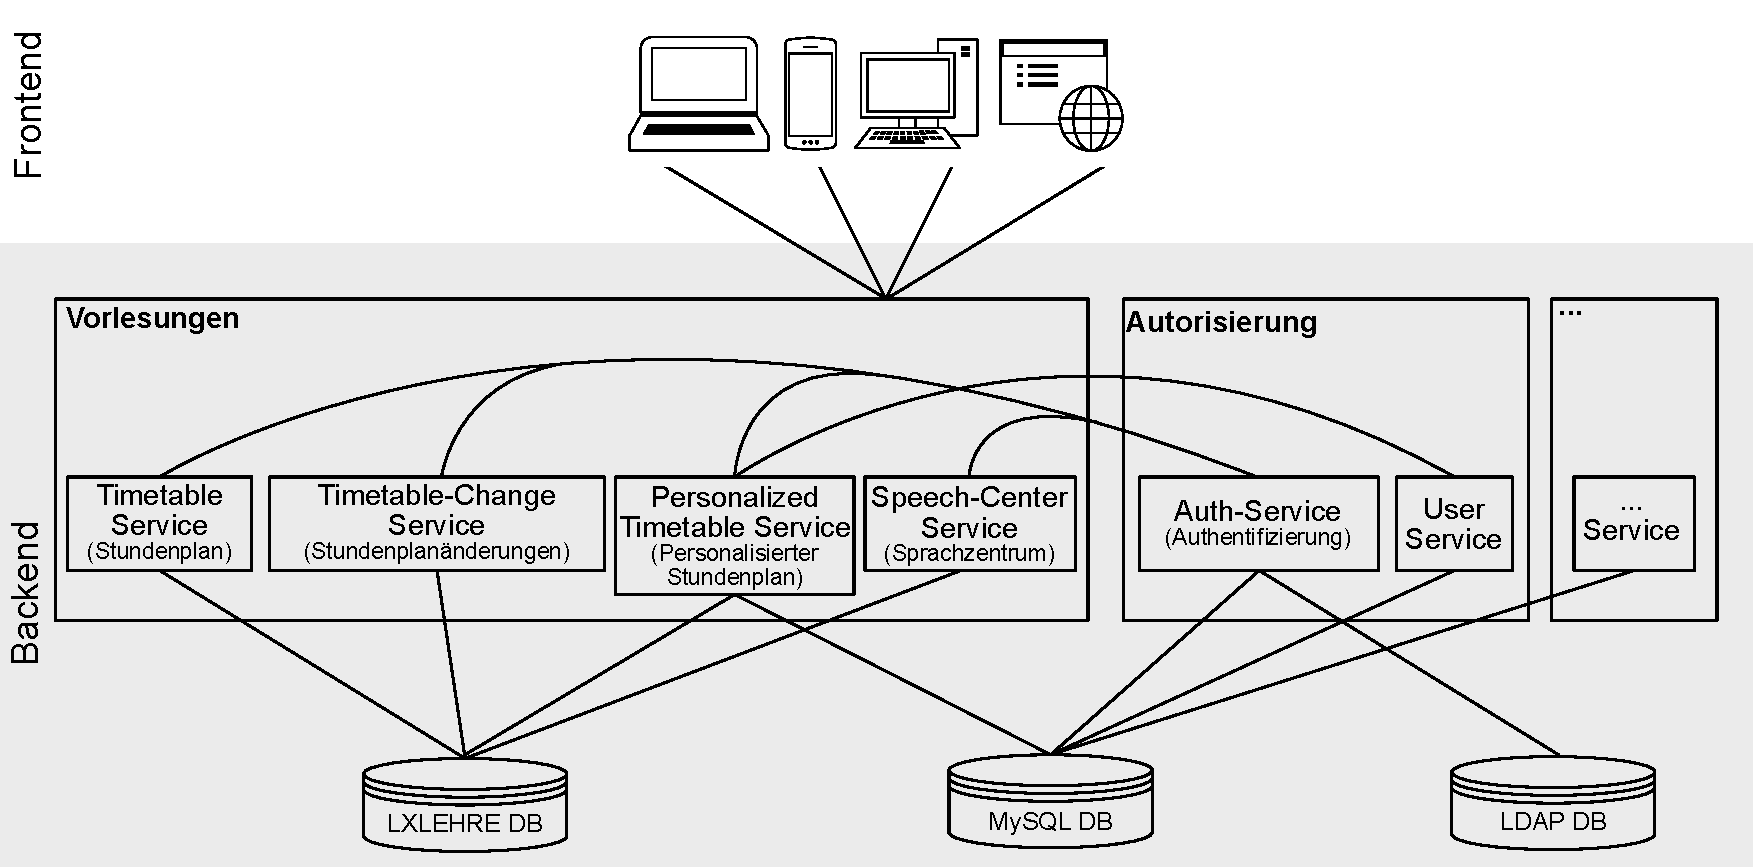
\includegraphics[,width=\pictureWidth cm + 2 cm]{Bilder/Architektur/SOA_FH_App_Architektur.pdf}
\caption{SOA Hochschul-App Architektur\label{fig:soaarch}\protect\footnotemark}
\end{figure}
\footnotetext{Brysiuk, Lehmann (2019)}


Zu erkennen ist einerseits, dass die Funktionalitäten der Anwendung in Services ausgelagert werden, die durch Module im Sourcecode getrennt sind und somit auch getrennt entwickelt werden können, jedoch nach dem Build-Prozess des Programmes in eine Komponente zusammengefasst werden. Die Entwicklung der Schnittstelle bleibt somit modular und flexibel, jedoch ist das Endprodukt nach jeder Änderung nach wie vor ein großer Monolith. Die Auslagerung und unabhängige Funktion der Services ist somit nicht gegeben, die Services können nicht nach deren Benutzungsstatistiken skaliert werden, lediglich die gesamte Anwendung könnte mehrmals parallel laufen, was aber weniger genutzte Teile der Anwendung ebenfalls hoch skalieren würde, was wiederum eine hohe Ressourcenverschwendung und hohe Kosten mit sich ziehen würde.
\\
\linebreak
Andererseits ist zu erkennen, das die Service-orientierte Architektur ebenfalls eine Abhängigkeit der einzelnen Services mit sich bringt. Bei einem Request müssen die Services Informationen untereinander austauschen können. So würde ein Request an den \textit{personalisierten Stundenplan} in der Service-orientierten Architektur die Folge haben, dass der Service zusätzlich Informationen vom \textit{User Service} benötigen würde um den Request verarbeiten zu können. Das erschafft Abhängigkeiten, durch die einzelne Services möglicherweise nicht mehr funktionieren, wenn sie benötigte Informationen nicht zurückerhalten. Außerdem ist zu erkennen, dass die Datenbank unter den Services geteilt wird. Durch die Verwendung einer gleicher Datenbank von mehreren Services könnten sogenannte \textit{Deadlocks} verursacht werden. Durch die bereits vorhandene Abhängigkeiten zwischen den Services wird die Ausfallwahrscheinlichkeit der Funktionalitäten durch diese \textit{Deadlocks} weiter verstärkt. Die Skalierung der Anwendung wird das Problem nicht lösen können, sondern im Gegenteil sogar verschlechtern, denn es entstehen immer mehr Instanzen die sich die gleichen Ressourcen teilen müssen.
\\
\linebreak
Um die Abhängigkeiten zu reduzieren und weitere vorhandene Probleme von \ac{SOA} zu minimieren steht der Microservice Architektur Ansatz zur Verfügung.
%Dieses Problem wird durch den Microservice Ansatz behoben, wodurch die Abhängigkeiten fast vollständig aufgelöst werden können.

\section{Microservice Architektur}

Die Microservice Architektur kann das Problem der Abhängigkeiten zwischen den Services bis zu einem gewissen Grat eliminieren. Im Beispiel des \textit{personalisierten Stundenplans} aus Kapitel \ref{sec:arch_soa} würden die benötigten Informationen aus dem \textit{User Service} lediglich als Übergabeparameter bei der Anfrage an den Service übergeben werden. Um dies genauer zu verstehen, werden die Grundlagen der Microservice Architektur im folgenden kurz erläutert.

\subsection*{Microservice Konzept}

Die Grundidee der Microservice Architektur kann durch das eben angebrachte Beispiel gut erklärt werden. In der \ac{SOA} Architektur werden die Funktionalitäten schon einmal in einzelne Module, Services genannt, getrennt. Diese sind jedoch nur im Entwicklungsprozess getrennt, nicht im Produktionsbetrieb, denn nach dem Build-Prozess und dem Deployment auf dem Server bilden diese Services einen einzigen Monolithen, der, wie schon in Kapitel \ref{sec:arch_soa} erwähnt wurde, nur im ganzen skaliert und vervielfacht werden kann. 
\\
\linebreak
Microservices lösen dieses Problem, in dem sie jeden Service nicht nur als Modul im Sourcecode trennen, sondern auch im Produktionsbetrieb. Jeder Service wird somit als eigene Anwendung gepflegt und kann unabhängig von allen anderen Services laufen und Anfragen bearbeiten. Die Vorteile dieser Strategie liegen auf der Hand.
\\
\linebreak
Zum einen können die einzelnen Services, in der Microservice Architektur auch Microservices genannt, einzeln skaliert werden. Somit können Teile der Anwendung, welche stark belastet werden, gut hoch skaliert werden, ohne auch die Teile der Anwendung zu skalieren, die kaum genutzt werden. Jeder Microservice kann als eigenes unabhängiges Modul auf unterschiedlichen Servern ausgelagert werden oder - wie bereits in Kapitel \ref{ws:zf} erwähnt wurde - in Cloud-basierte-Plattformen verschoben werden oder als Docker-Container realisiert werden. Somit können die vorhandenen Ressourcen optimal genutzt werden. Zum anderen kann man die Ausfallsicherheit und die Sicherheit im allgemeinen deutlich erhöhen, wenn man nur die einzelnen Microservices redundant hält. Sollte ein Microservice ausfallen, so kann eine andere Instanz des Services einsetzen, sollte keine weitere Instanz verfügbar sein, so läuft der Rest der Anwendung trotzdem problemlos weiter, da die anderen Funktionalitäten in eigene Microservices ausgelagert werden, die komplett unabhängig voneinander laufen. Somit werden durch die Microservice Architektur einige wichtige nicht-funktionale Anforderungen wie die Skalierbarkeit, Performance und Verfügbarkeit deutlich erweitert.  
\\
\linebreak
Aber auch \ac{DoS} und \ac{DDoS} Angriffe können einfacher kompensiert werden. Sollte keine Sicherheitsmaßnahme getroffen  werden, die solche Attacken frühzeitig erkennen, so würde bei einem Angriff auf einen einzelnen Microservice nur diese Funktionalität betroffen sein, die anderen Services, die unabhängig davon laufen, sind nicht gefährdet. Außerdem wird durch die erweiterte Modularisierung und Auflösung der Abhängigkeiten zwischen den Funktionalitäten das Testen, die Fehlerbehebung und die Erweiterungen der Funktionalitäten erleichtert. Die begründet sich einerseits, weil die Microservices leichtgewichtiger gestaltet sind, was die Erweiterbarkeit, Veränderbarkeit und Austauschbarkeit erleichtert, andererseits dadurch, dass durch die geringeren Abhängigkeiten die Komplexität der Funktionalitäten gemindert wird. Zusätzlich kann und sollte ebenfalls ein \ac{API}-Gateway genutzt werden, welches die Anfragen auf die einzelnen Microservices kontrolliert und nochmals eine Sicherheitsbarriere darstellt, sowie die einzelnen Microservices zu einer ganzen Anwendung verbindet. Wo diese in der Anwendung einzubinden ist, zeigt Abbildung \ref{fig:architektur_app}, genaueres zum \ac{API}-Gateway wird noch in Kapitel \ref{sec:api_gateway} erläutert. 

\begin{figure}[H]
\centering
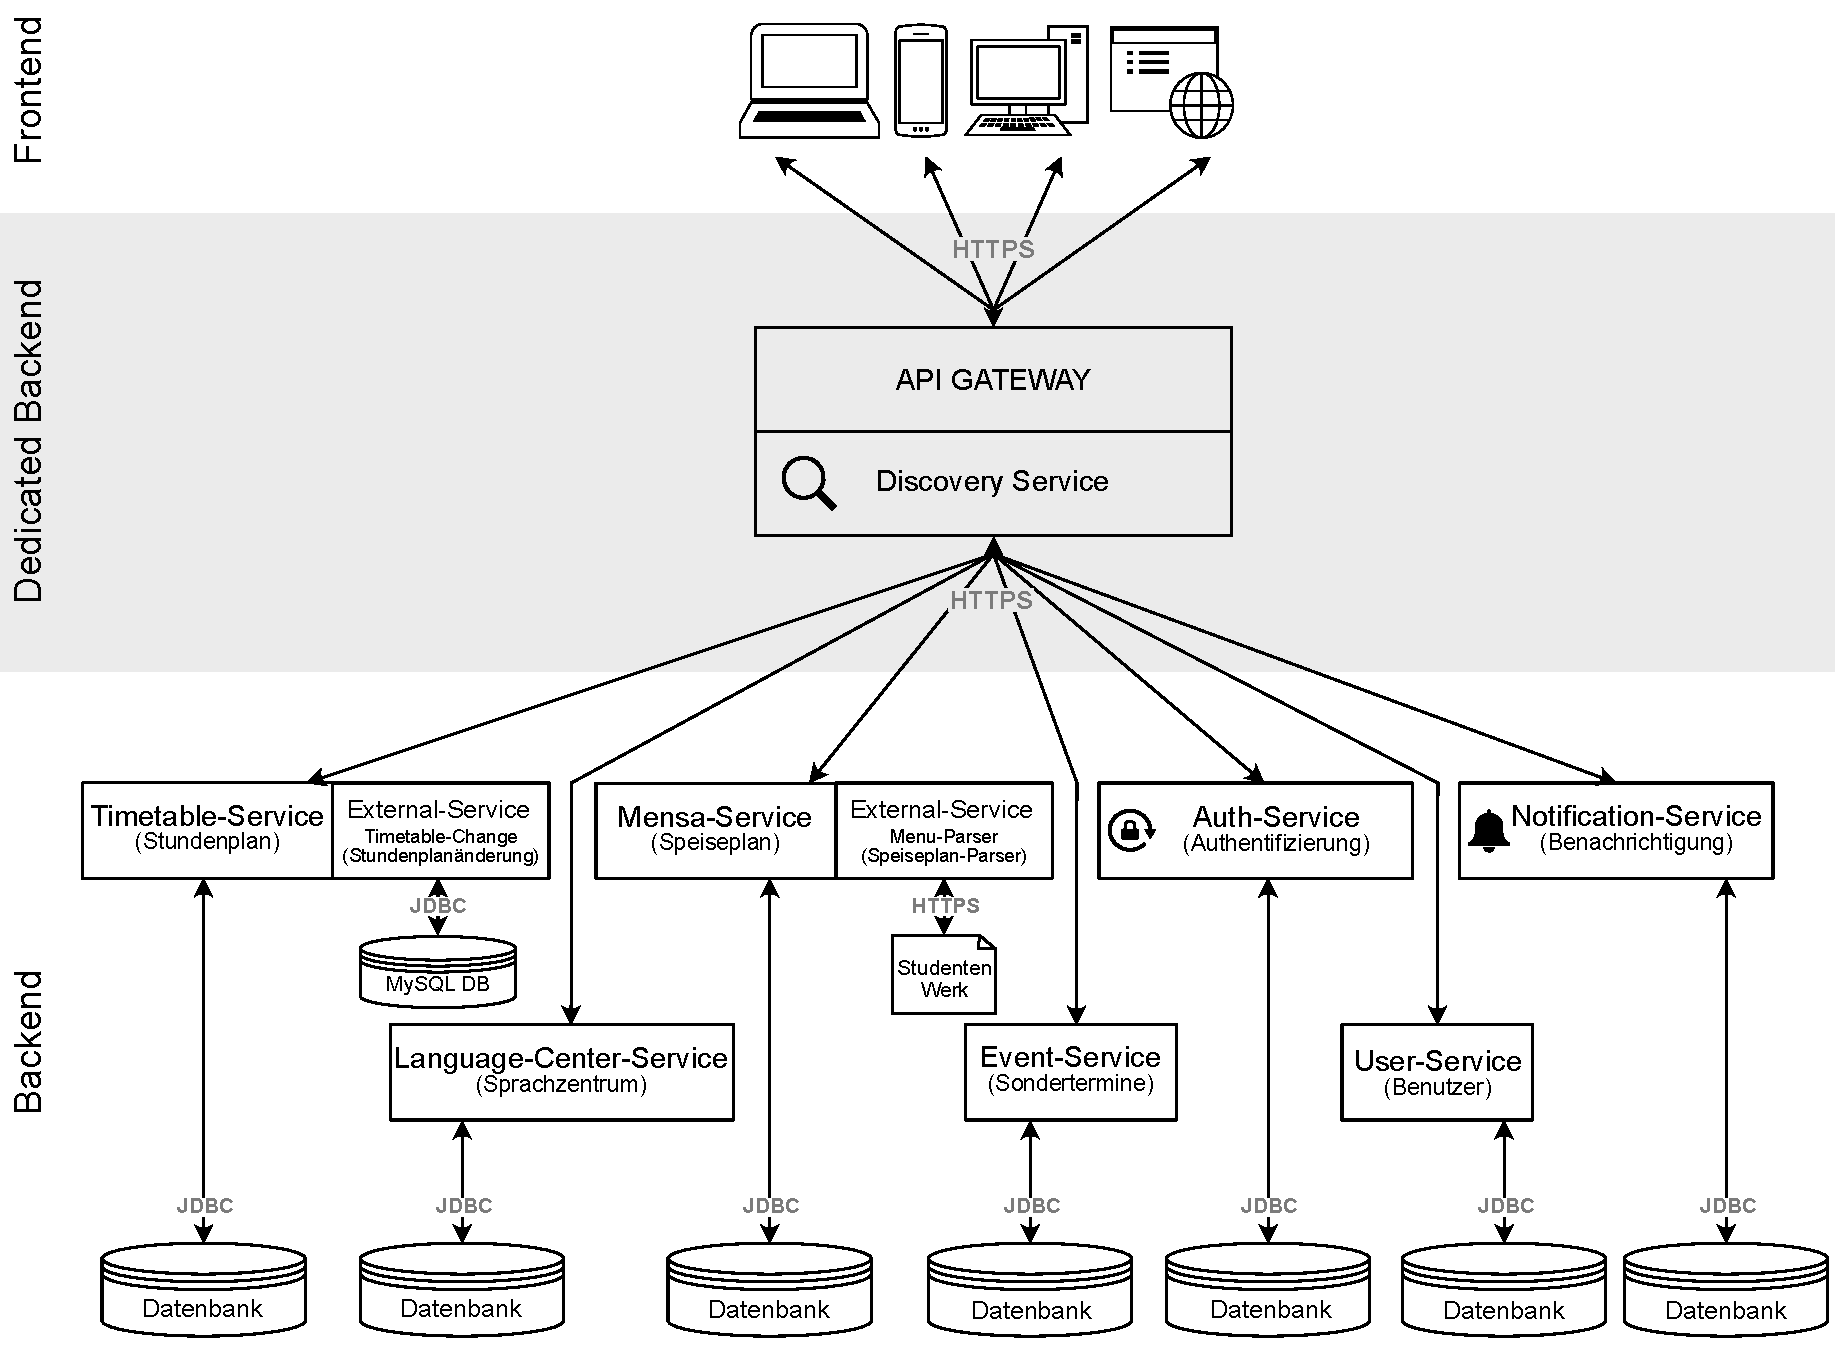
\includegraphics[,width=\pictureWidth cm + 2 cm]{Bilder/Architektur/MS_FH_App_Architektur.pdf}
\caption{Microservices Hochschul-App Architektur\label{fig:architektur_app}\protect\footnotemark}
\end{figure}
\footnotetext{Brysiuk, Lehmann (2019)}


Wie auf Abbildung \ref{fig:architektur_app} ebenfalls zu erkennen ist, wurden die einzelnen Anforderungen aus Kapitel \ref{sec:anforderung} in kleine unabhängige Microservices mit jeweils einer eigenen Datenbank getrennt. Das erfordert zwar, dass man mehrere Systeme aufsetzen muss, was mehr Aufwand in der Entwicklung bedeutet, jedoch kann man die Microservices und Datenbanken an die Bedürfnisse der einzelnen Funktionen anpassen und dementsprechend optimieren. So muss zum Beispiel nicht jeder Service auf die gleiche Art von Datenbank zurückgreifen, sonder kann die Art nutzen, die seine Anforderungen am besten erfüllt. Dies kann beispielsweise eine \ac{NoSQL}-Datenbank statt einer klassischen relationalen Datenbank sein, was bei einer \ac{SOA}-Architektur deutlich aufwändiger wäre, da dafür andere Schnittstellen in der Persistenz der Anwendung benötigt werden. Die Definition und die Spezifikation der einzelnen Microservices wird später noch in Kapitel \ref{sec:appservices} behandelt. 

\subsection*{Discovery Service\label{sec:discovery}}

Die Grundidee der Microservice Architektur zielt in großen Teilen auf die Skalierbarkeit und die gekapselte Zuständigkeit der einzelnen Services ab. Dieser Grundsatz beinhaltet im Wesentlichen zwei Teile. Einerseits möchte man bei der Kapselung der Zuständigkeiten der einzelnen Services erreichen, dass sowohl die Entwicklung, als auch der Produktionsbetrieb dieser Einzelteile unabhängig verlaufen können. Dabei spielen auch die physische Adresse und der Deployment-Server eine Rolle, denn einem Service, der gestartet wird, muss auch eine Adresse vergeben werden, mit er er angesprochen wird. Bei diesem Prozess spielt der \textit{Discovery Service} eine maßgebliche Rolle. Er bietet einen Anlaufpunkt, bei dem sich alle anderen Services mit ihrer Adresse registrieren können. Wird dann ein Service benötigt, so muss man den Discovery Service nur nach der Bezeichnung des Services fragen, worauf dieser dann mit der Adresse des gesuchten Services antwortet. 
\\
\linebreak
Andererseits möchte man bei der Aufteilung der Services erreichen, dass die einzelnen Instanzen optimal ausgelastet werden. So kann es bei der neuen Hochschul-Anwendung zum Beispiel vorkommen, dass der Stundenplan-Service stark ausgelastet ist, da das die zentrale Aufgabe dieser \ac{App} sein soll. Man kann bei Überlastungen dieses Services sehr einfach weitere Instanzen dessen auf anderen physikalischen Geräten deployen, um die Last gleichmäßig zu verteilen. Jedoch muss man nun einen Dienst einbinden, welcher die Adressen dieser Instanzen kennt und auch im Auge behält, welcher Dienst wie stark ausgelastet ist. Auch diese Aufgabe übernimmt der Discovery Service. Da sich alle Instanzen der Services mit ihrer Bezeichnung bei dem Discovery Service registrieren kann dieser die verschiedenen Instanzen des gleichen Services gruppieren und die Anfragen gleichmäßig verteilen. Der Client ruft dafür nur die Bezeichnung des Services beim Discovery Service ab und bekommt  darauf die Adresse des Services, der diese Aufgabe erledigt und der aktuell am wenigsten ausgelastet ist.
\\
\linebreak
Um diesen Discovery Service sinnvoll nutzen zu können, benötigt die Anwendung ein \ac{API}-Gateway, welches sich ebenfalls als Service beim Discovery Service registriert. Auch für dieses Gateway gilt, dass sich mehrere Instanzen registrieren können. Auch dieser Teil der Anwendung kann somit skaliert werden. Das \ac{API}-Gateway ruft dann für einen Client die Services beim Discovery Service ab. Die genaue Funktion des Gateways werden im Kapitel \ref{sec:api_gateway} \textit{API-Gateway} betrachtet. 

\subsection*{API-Gateway\label{sec:api_gateway}}

Als Verbindungsstück zwischen den Services und ihrer einzelnen Instanzen fungiert der im vorigen Kapitel \ref{sec:discovery} \textit{Discovery Service} beschriebene Service. Der große Vorteil dessen ist, dass man lediglich die Adresse des Discovery Services benötigt, um dann mit allen anderen Microservices zu kommunizieren. Um einem externen Client jedoch die Möglichkeit zu geben, die Vorteile dessen nutzen zu können, benötigt es ein \ac{API}-Gateway, bei dem der Nutzer die gewünschten Ressourcen anfragt und das sich dann um die Beschaffung dieser kümmert. Somit muss auch der Client nicht mehr jede Adresse der Services kennen, sondern nur die des\ac{API}-Gateways. Dies führt einerseits zu sauberem Code, da eine echte Adresse nicht mehr fest im Programmcode eingegeben werden muss, andererseits auch zu einer Möglichkeit, den Zugriff auf die Funktionen des Discovery Services und alle darunter liegenden Microservices zu kontrollieren.
\\
\linebreak
Die Funktion des \ac{API}-Gateways und der Zusammenarbeit des Discovery Services mit diesem werden in Abbildung \ref{fig:discovery_seq} gezeigt.

\begin{figure}[H]
\centering
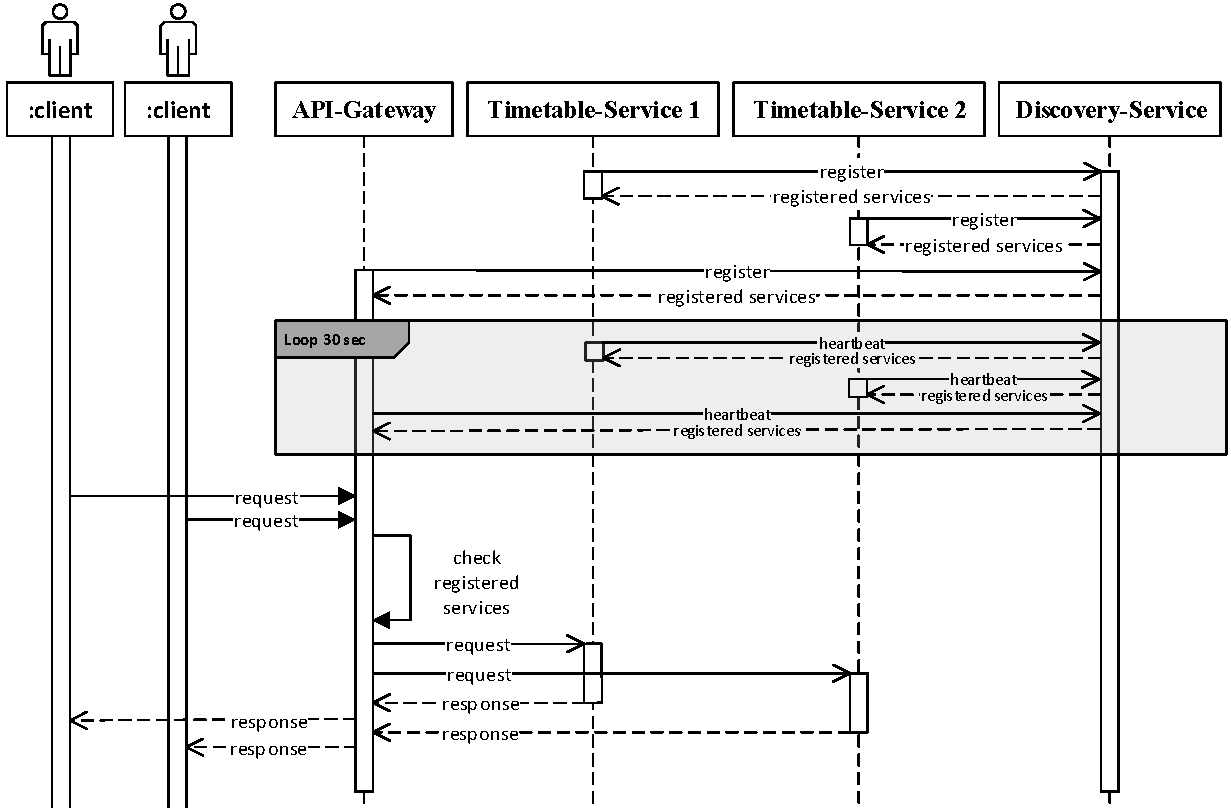
\includegraphics[,width=\pictureWidth cm + 2 cm]{Bilder/Sequenz_Diagramm/Discovery_Sequenz.pdf}
\caption{Sequenzdiagramm zwischen Discovery, \ac{API}-GATEWAY und Services\label{fig:discovery_seq}\protect\footnotemark}
\end{figure}
\footnotetext{Brysiuk, Lehmann (2019)}


Wie zu erkennen ist, registrieren sich alle Services, das \ac{API}-Gateway eingeschlossen, beim Discovery Service, welcher diesen dann eine Liste der aktuell registrierten Services und deren Adressen zurückgibt. Diese Liste wird in jedem Service gespeichert. Nach der erfolgreichen Registrierung melden sich die Services dann alle 30 Sekunden wieder beim Discovery Service, der dann wieder eine aktualisiert Liste zurückgibt. Dieses wiederholte Melden und Aktualisieren nennt man den \textit{Heartbeat} der registrierten Services. Sollte dieser Heartbeat einmal ausfallen, so entfernt der Discovery Service den Service, der sich nicht mehr meldet, automatisch nach einem definiertem Threshold an Fehlversuchen. 
\\
\linebreak
Sobald das \ac{API}-Gateway sich beim Discovery Service registriert hat, können die Clients erfolgreiche Anfragen an dieses schicken. Je nach Anfrage überprüft das Gateway dann, welcher passende Service bei ihm in der Liste, die er vom Discovery Service erhalten hat, enthalten ist und spricht diesen dann direkt mit der hinterlegten Adresse an. Die Antwort bekommt dieser darauf direkt vom angesprochenen Service, die Kommunikation läuft somit direkt zwischen den betroffenen Services, was die Performanz deutlich steigert. Lediglich die Registrierung und der Austausch der Adressen läuft parallel dazu im Hintergrund über den Discovery Service. 

\section{Schichtenarchitektur\label{sec:schichtenarchitektur}}

Wie bereit in Kapitel \ref{sec:layering} beschrieben wurde, soll die Architektur in Schichten aufgeteilt sein, um die Zuständigkeiten der einzelnen Funktionalitäten des Softwaresystems zu trennen und modular zu halten. Im Falle der Web-basierten Hochschul-\ac{App} trifft das auf die Architekturen der einzelnen Microservices zu. Diese werden, wie in Abbildung \ref{fig:ms_layer_alg} gezeigt, in 4 Schichten aufgeteilt, von denen eine nochmals physisch ausgelagert werden kann.

\begin{figure}[H]
\centering
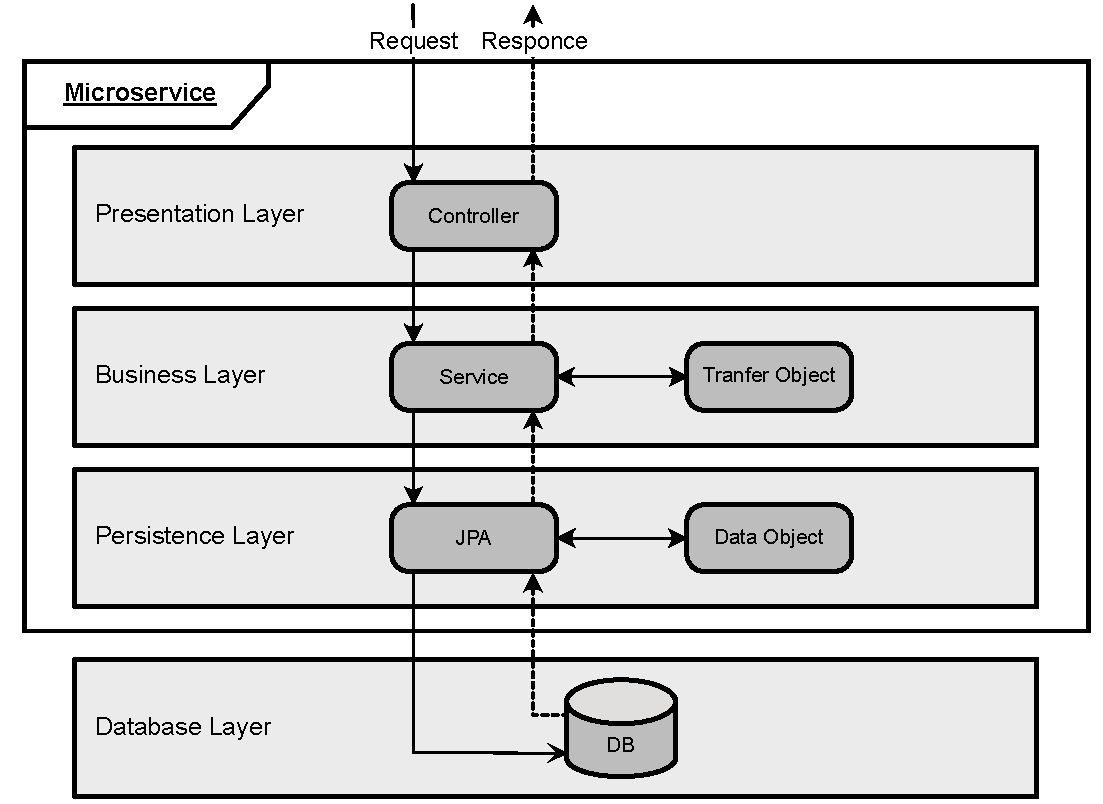
\includegraphics[,width=\pictureWidth cm]{Bilder/Architektur/MS_Schichtenarchitektur.pdf}
\caption{Microservice in Schichten Aufgeteilt\label{fig:ms_layer_alg}\protect\footnotemark}
\end{figure}
\footnotetext{Brysiuk, Lehmann (2019)}

Konkret übernehmen die Schichten folgende Aufgaben:

\begin{itemize}

\item \textbf{Presentation Layer} 
\\
Wie der Name der Schicht schon sagt, ist diese Schicht für die äußerliche Darstellung der Anwendung zuständig. Im Falle einer \ac{REST}-Schnittstelle sind das die Endpunkte, über die ein Client Daten abfragen kann. Diese Schicht ist nur für die Schnittstelle zuständig, sie definiert also die \acp{URL} für die Endpunkte und sichert die Anwendung nach außen ab. Zudem leitet sie die Anfragen an die darunterliegende Schicht, die Business Schicht, weiter.

\item \textbf{Business Layer} 
\\
Die Business Schicht übernimmt die eigentliche Aufgabe, für die die Anwendung geschrieben wurde. Sie enthält also die Kernlogik des Systems. Alle Algorithmen und Datenverarbeitungen werden in dieser Schicht durchgeführt. Benötigt eine dieser Vorgänge Daten, so werden diese aus der darunter liegenden Schicht, der Persistenz Schicht, abgefragt.

\item \textbf{Persistence Layer}
\\
Die Persistenz Schicht hat im Grunde nur zwei Aufgaben, Daten auszulesen und Daten zu speichern. Um die Datenquellen vor der Business Schicht zu verstecken und den Zugriff für alle Quellen zu vereinheitlichen bietet diese Schicht eine einheitliche Schnittstelle für die Daten aus allen Datenquellen. Wenn die Business Schicht die gelesenen Daten ändern möchte oder neue Daten einspeisen will, so kann sie das auch über die Persistenz Schicht tun. In diesem Fall gilt das gleiche Prinzip, wie beim Auslesen. Die Schnittstelle wird für alle Datenquellen angeglichen. So muss beim Austausch der Datenquellen nur die Persistenz Schicht, nie eine der darüber liegenden Schichten angepasst werden.

\item \textbf{Database Layer}
\\
Diese Schicht ist im Rahmen der Schichtenarchitektur nicht zwingend notwendig, allerdings wird sie im Großteil der Services der Hochschul-\ac{App} angewendet. Sie bildet die Grundlage der Datenschnittstelle der Services, die Datenbank. Die Datenbank ist kein Teil des eigentlichen Sourcecodes der Anwendung und kann somit separat zur Anwendung gepflegt werden. Jedoch kann die Anwendung ohne die Datenbank keine Daten bereitstellen, somit ist die Datenbank Schicht für die Hochschul-\ac{App} unverzichtbar.

\end{itemize}

\subsection*{Ablauf einer Anfrage}

Eine Anfrage eines Clients durchläuft im allgemeinen immer den selben Ablauf. Die Anfrage selbst wird an einen Endpunkt gerichtet, der durch eine \ac{URL} definiert wurde. Die Präsentations Schicht greift diese Anfrage auf und untersucht, ob der Client, der die Anfrage gestellt hat, die nötigen Berechtigungen für den Zugriff hat.
\\
\linebreak
Trifft das zu, so wird die Anfrage an die Business Schicht weitergeleitet, welche sie dann verarbeitet. Benötigt die Business Schicht zum Bearbeiten der Anfrage weitere Daten, so fragt sie diese in der Persistenz Schicht ab. Die Persistenz Schicht kann dann unterscheiden, um welche Art von Daten es sich handelt und wo diese zu finden sind. Sind die Daten aus der Datenbank auszulesen, so werden diese in der Datenbank Schicht abgefragt. Es kann sich aber auch um Daten handeln, welche von einem externen Anbieter geholt werden müssen. In diesem Fall schickt die Persistenz Schicht eine Anfrage an die Schnittstelle des externen Anbieters und liefert dann die Daten an die Business Schicht zurück. Die Daten werden zwischen der Persistenz Schicht und der Business Schicht immer in sogenannten \textit{Data Objects}, manchmal auch \textit{Business Entities} genannt, gekapselt. In der Programmiersprache Java werden diese Wrapper Objekte typischerweise mit dem Namen der Datenart, gefolgt von den Buchstaben \textit{\ac{DO}} benannt. 
\\
\linebreak
Die Business Schicht verarbeitet die Daten dann dementsprechend. Die veränderten Daten können dort auch wieder an die Persistenz Schicht weitergegeben werden, wo sie dann wieder in der zugehörigen Datenquelle abgespeichert werden. Im Falle der Hochschul-\ac{App} werden die Daten wieder in der Datenbank persistiert. Die Daten, die die Präsentations Schicht zur Beantwortung der Anfrage des Client benötigt, werden dann wieder von der Business Schicht an die Präsentations Schicht zurückgegeben. Diese Daten werden in \textit{Transfer Objects} weitergegeben. Hier werden die Wrapper Klassen in Java typischerweise mit dem Namen gefolgt von den Buchstaben \textit{\ac{TO}} benannt. 
\\
\linebreak
Die Antwort der Business Schicht an die Präsentations Schicht hängt immer von der Anfrage ab. Es können sowohl echte Daten, als auch nur Erfolgs-/ Misserfolgsbenachrichtigungen zurückgeliefert werden. Sollten Daten zurückgeliefert werden, so immer in Form von \textit{Transfer Objects}. Fehlermeldungen werden in in Java oft als Exceptions zurückgeliefert, in anderen Programmiersprachen mit ähnlichen Konstrukten. Erfolge werden meist durch Boolesche Werte oder durch das zurückkehren ohne Fehlermeldung signalisiert. Die empfangenen Rückgabewerte werden dann von der Präsentations Schicht an den Client zurückgegeben.
\\
\linebreak
Die Unterscheidung von \textit{Transfer Objects} und \textit{Data Objects} ist deshalb nötig, da in der Business Schicht oft Daten aus der Persistenz Schicht benötigt werden, die der Client entweder nicht einsehen darf, oder die er nicht verarbeiten kann. Deshalb werden die Daten, die über die Schnittstelle der Präsentations Schicht an den Client gehen, immer so bearbeitet, dass sie in der richtigen Form sind und keine sensiblen Daten mehr enthalten.

\subsection*{Aufbau der anwendungsinternen Schichten}

In Abbildung \ref{fig:ms_layer_alg} werden die groben Schichten der kompletten Software Architektur der Services und ihre Aufgaben betrachtet. Abbildung \ref{fig:ms_layer} hingegen betrachtet den Aufbau der drei oberen Schichten, die im Sourcecode der Anwendung liegen. Die Datenbank Schicht wird hierbei nicht weiter betrachtet. 

\subsubsection*{Package Struktur}

Ähnlich, wie die Schichten der Anwendung, wird auch der Programmcode unterteilt. Wie bereits in Kapitel \ref{sec:schichtenarchitektur} beschrieben wurde, sind die oberen drei Schichten auch im Sourcecode der Hochschul-\ac{App} zu finden. Die Package Struktur dieser richtet sich nach den drei Schichten, so gibt es ein Presentation Package, ein Business Package und ein Persistence Package. 
\\
\linebreak
Das Controller Package ist, wie zu erahnen ist, für die Endpunkte der Anwendung zuständig. In Microservice Anwendungen nennt man die zugehörigen Klassen oder Handler oft Controller, da es \ac{REST}-Schnittstellen sind, auch \ac{REST}-Controller. Demnach richtet sich auch die Namenskonvention. Den Anfang des Namens macht der Name der Schnittstelle, in Abbildung \ref{fig:ms_layer} beispielhaft \textit{Test} genannt, darauf folgend wird das Wort \textit{Controller} angehängt. Für jeden Teil der Schnittstelle kann man einen eigenen Controller definieren, so wird der Code auch übersichtlicher. 
\\
\linebreak
Das Service Package enthält alle Algorithmen zur Datenverarbeitung. Auch hier ist die Namenskonvention ähnlich wie im Controller Package aufgebaut, jedoch nennt man die zugehörigen Klassen oder Handler hier \textit{Services}. Der Namen beginnt auch hier mit dem Namen des Services und endet mit \textit{Service}. Zusätzlich zu den Services enthält dieses Package auch die in Kapitel \ref{sec:schichtenarchitektur} erwähnten \textit{Transfer Objects}. Diese werden im untergeordneten Package \textit{TransferObject} definiert. Die zugehörige Namenskonvention wurde bereits erläutert.
\\
\linebreak
Das letzte Package, das sich nach der allgemeinen Schichtenarchitektur richtet, ist das Repository Package. Hier werden die Daten aus den verschiedenen Datenquellen gesammelt. Die Namenskonvention ist hier unterschiedlich, je nachdem, um welche Art von Datenquelle es sich handelt. Bei nativen \ac{SQL}-Statements werden die zuständigen Klassen oder Handler oft \textit{DatabaseAccessor} oder \textit{[Name]Accessor} genannt. Bei externen Schnittstellen wird oft der Name gefolgt von der Abkürzung \textit{\ac{API}} genutzt. Bei der Nutzung der \ac{JPA} wir der Name der Datenquelle gefolgt von der Abkürzung \textit{\ac{JPA}} verwendet. Im Repository Package werden, wie in der Persistenz Schicht definiert wurde, auch die \textit{Data Objects} in einem untergeordneten Package gelagert. Auch für diese wurde die Namenskonvention bereits dargestellt. 
\\
\linebreak
Um die Aufgaben des Services von anderen Hilfsbibliotheken oder Prozeduren zu trennen benötigt die Package Struktur der Hochschul-\ac{App} und von Microservices im Allgemeinen noch weitere Packages für externes. Darunter gehören zum Beispiel externe Services, die man nicht ganz von der Aufgabe des Microservices trennen kann, die aber auch nicht direkt dazugehören. Ein Beispiel dafür ist der Zugriff auf eine externe Schnittstelle eines anderen Anbieters. Der Zugriff an sich wird dabei von einer externen Bibliothek durchgeführt. Ein weiteres Package ist das \textit{Util} Package. Dieses beinhaltet Hilfsbibliotheken und Klassen. Ein Beispiel hierfür sind Datenparser, welche gelesene Daten in ein einheitliches Format bringen.

\begin{figure}[H]
\centering
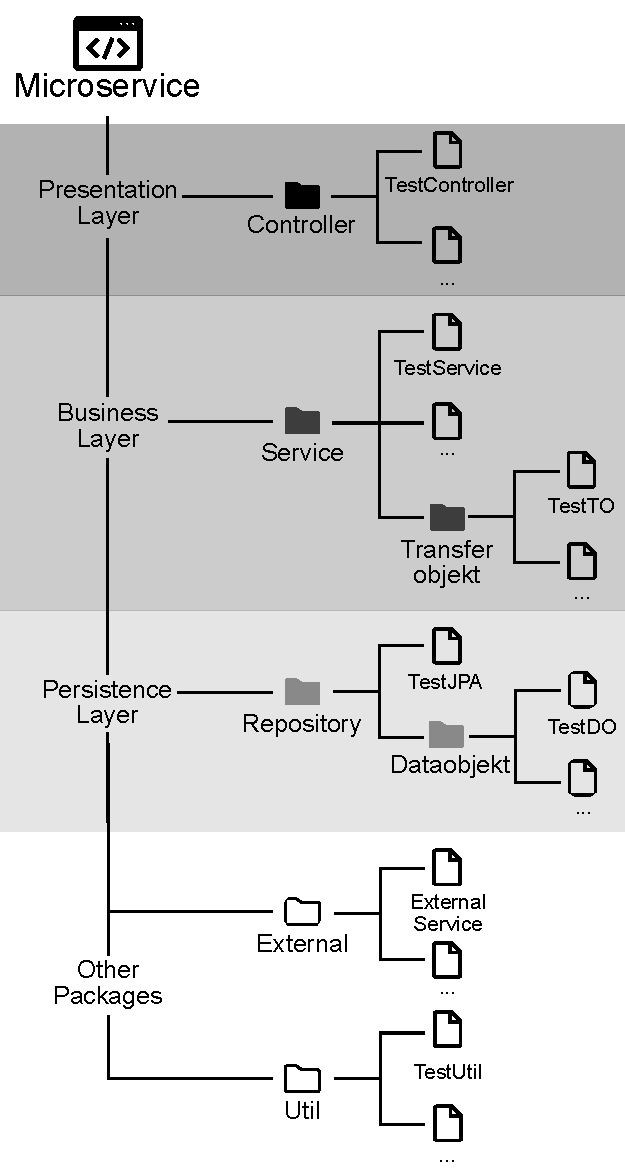
\includegraphics[,width=\pictureWidth cm -6 cm]{Bilder/Architektur/MS_Pakage_Stuktur.pdf}
\caption{Microservice Schichtenarchitektur\label{fig:ms_layer}\protect\footnotemark}
\end{figure}
\footnotetext{Brysiuk, Lehmann (2019)}



% App Services
\chapter{Services der Hochschul-App}
\label{sec:appservices}
%Text

Wie im vorhergehenden Kapitel \ref{sec:architektur} bereits beschrieben wurde, basiert eine Microservice Architektur darauf, dass man einzelne Funktionalitäten der Anwendung in einzelne Services aufteilt. Die allgemeinen Richtlinien bei der Erstellung einer Web Service Architektur wurden ebenfalls schon im Kapitel \ref{sec:webservices} zum Thema Web Services beschrieben. 
\\
\linebreak
Im Allgemeinen werden die Services der Datenschnittstelle der neuen Hochschul App anhand der funktionalen Anforderungen und der architekturbedingten Vorgaben aufgeteilt. Die Services für den Stundenplan, die Stundenplanänderungen, den Mensaplan, die Benachrichtigungen und der Authentifikation bilden einzelne Services, die sich nach der entsprechenden funktionalen Anforderung richten. Die Namensgebung beschreibt hier in dem Fall schon eindeutig, welche Aufgaben jeder einzelne Service erfüllt. Die eindeutige Namensgebung trifft in diesem Fall auch auf den Anwenderservice zu, welcher sich jedoch weniger nach den funktionalen Anforderungen richtet, sondern vielmehr an den technischen Vorgaben der Microservice Architektur. In diesem Fall wird eine Funktion der Anwendung so ausgelagert, dass keine der anderen Services von diesem einen Service abhängig sind. Dieser Service ermöglicht es dennoch, die Funktion der Anwenderverwaltung zu kapseln und somit redundanten Programmcode weitgehend zu vermeiden. Die genauen Anforderungen an die einzelnen Services, deren Funktionsweise und Aufbau, sowie die grundlegende Struktur der dahinter liegenden Daten werden im folgenden genauer erarbeitet.  

% Stundenplan
\section{Stundenplan (Timetable-Service)}
\label{sec:stundenplan}
% Text

Die wichtigste Funktion der Hochschul-App soll es sein, den Stundenplan leichter für mobile Endgeräte darzustellen. Wie bereits in den vorhandenen Anwendungen der Hochschule Hof baut auf dieser Funktion die komplette Anwendung auf. Demnach ist es wichtig, dass die Erarbeitung dieser zentralen funktionalen Anforderung unter höchster Sorgfalt geschieht. Diese beinhaltet nicht nur die Bereitstellung des allgemeinen Stundenplans zum Verlesungsangebot der Hochschule, sondern auch die Möglichkeit, personalisierte Anfragen an die Datenquelle zu stellen, die in einer grafischen Oberfläche ebenfalls in einen personalisierten Stundenplan umgewandelt werden können. 

% Stundenplan Anforderung
\subsection*{Anforderung an Schnittstelle}
\label{sec:stundenplan_anforderung}
% Text

Die Daten zum Vorlesungsangebot der Hochschule Hof werden separat zur Anwendung in einer Datenbank gehalten und gepflegt. Zur Nutzung dieser und zum Arbeiten mit den Daten werden diese allerdings in modifizierter Form in einer eigenen Datenbank abgelegt. Die Schnittstelle des Services muss dem Client alle relevanten Daten zu den einzelnen Vorlesungen geben. Diese Vorlesungen kann der Client einzeln oder in verschiedenen Listen abfragen. 
\\
\linebreak
Jede einzelne Vorlesung muss mindestens folgende Informationen liefern:

\begin{itemize}

\item Eine eindeutige Kennung der Vorlesung (ID)

\item Der Name der Vorlesung

\item Die Art der Vorlesung

\item Dozent der Veranstaltung

\item Start und Ende der Vorlesung (speziell für Block-/ Sonderveranstaltungen)

\item Vorlesungszeiten

\item Die Studiengänge, in denen die Vorlesung angeboten wird

\item Fachsemester der Vorlesung

\item Vorlesungsraum

\end{itemize}

Die Daten lassen sich in allgemeine Informationen zur Veranstaltung, zeitliche Einschränkungen und in Informationen zum Rahmen der Vorlesung aufteilen. Beim Abfragen der Daten muss der Client die Möglichkeit haben, eine Liste von Veranstaltungen anhand von verschiedenen Suchkriterien zu erhalten. Möchte ein möglicher Nutzer demnach seinen aktuellen Stundenplan abfragen, so muss der Client eine Anfrage stellen können, die den Studiengang und das Fachsemester enthält. Die Antwort muss dann das komplette Vorlesungsangebot für diesen Nutzer enthalten. Ähnlich verhält es sich bei Suchen nach speziellen Vorlesungen. Es muss möglich sein, eine Liste an Vorlesungen zu erhalten, die gewisse Suchkriterien erfüllen. Möchte der Client demnach eine Liste aller Vorlesungen eines Dozenten haben, oder alle Veranstaltungen zu einem gewissen Zeitpunkt abfragen, so muss er das tun, indem er diese Suchkriterien in der Anfrage angibt. 
\\
\linebreak
Anders als beim personalisierten Stundenplan gibt der Client bei einem allgemeinen Stundenplan eine Anfrage ab, bei der er nicht weiß, welche und wie viele Ergebnisse er zurückerhält. Möchte der Client allerdings die in einem personalisierten Stundenplan abgelegten Vorlesungen abfragen, so muss er eine Anfrage stellen, in der alle eindeutigen Kennzeichnungen der Vorlesungen enthalten sind. Solang eine Kennung auch existiert, muss die Schnittstelle die zugehörigen Daten auch zurückgeben.

% Stundenplan Umsetzung
\subsection*{Spezifikation der Ressourcen}
\label{sec:stundenplan_api}
% Text 

In den GET-Methoden der Subresource /room/\{room\} können im Body die Filter für Uhrzeit, Datum oder Wochentag übergeben werden. Für die restlichen Subresourcen, außer /\{id\} und /\{name\}, können Filter für Dozent, Uhrzeit, Vorlesungssprache, Art der Vorlesung und Datum oder Wochentag übergeben werden. Die Filter Parameter sind optional, ohne eine Übergabe der Filter werden standardmäßig alle Vorlesungen zurückgegeben.  

\begin{itemize}
\item \subsubsection{GET/POST/DELETE:\\ /lectures} 
Die Methode GET liefert alle Vorlesungen unter der Berücksichtigung von gesetzten Filtern. POST erlaubt erstellen von einer oder mehreren Vorlesungen und DELETE löscht alle Vorlesungen.

\item \subsubsection{GET/PATCH/DELETE:\\ /lectures/\{id\}} 
Die Methode GET liefert eine Vorlesung für die übergebende ID. Mit PATCH kann die Vorlesung geändert beziehungsweise korrigiert werden und DELETE löscht diese Vorlesung.

\item \subsubsection{GET:\\ /lectures/\{lecture\}} 
Liefert eine Vorlesung unter der Berücksichtigung von übergebenen Vorlesungsbezeichnung.
\item \subsubsection{GET/POST/DELETE:\\ /lectures/faculty} 
Die Methode GET liefert eine Liste vorhandener Fakultäten. POST erlaubt die Fakultätsliste zu erweitern und DELETE löscht die komplette Fakultätsliste.
\item \subsubsection{GET/PATCH/DELETE:\\ /lectures/faculty/\{faculty\}} 
Die Methode GET liefert alle Vorlesungen die zur der übergebende Fakultät gehören. Mit PATCH kann die Fakultät geändert beziehungsweise korrigiert werden und DELETE löscht diese Fakultät aus der Fakultätsliste.
\item \subsubsection{GET/POST/DELETE:\\ /lectures/faculty/\{faculty\}/program} 
Die Methode GET liefert eine Liste vorhandener Studiengänge. POST erlaubt die Studiengangliste zu erweitern und DELETE löscht die komplette Studiengangliste.
\item \subsubsection{GET/PATCH/DELETE:\\ /lectures/faculty/\{faculty\}/program/\{program\}} 
Die Methode GET liefert alle Vorlesungen die zur gesetzten Fakultät und Studiengang gehören. Mit PATCH kann der Studiengang geändert beziehungsweise korrigiert werden und DELETE löscht diesen Studiengang aus der Studiengangliste.
\item \subsubsection{GET/POST/DELETE:\\ /lectures/faculty/\{faculty\}/program/\{program\}/semester} 
Die Methode GET liefert eine Liste vorhandener Semester. POST erlaubt die Semesterliste zu erweitern und DELETE löscht die komplette Semesterliste.
\item \subsubsection{GET/PATCH/DELETE:\\ /lectures/faculty/\{faculty\}/program/\{course\}/program/\{semester\}} 
Die Methode GET liefert alle Vorlesung die zur der gesetzten Fakultät, Studiengang und Semester gehören. Mit PATCH kann der Semester geändert beziehungsweise korrigiert werden und DELETE löscht diesen Semester aus der Semesterliste.

\item \subsubsection{GET:\\ /lectures/room} 
Liefert eine Liste vorhandener Vorlesungsräume.
\item \subsubsection{GET:\\ /lectures/room/\{room\}} 
Liefert alle Vorlesungen die zur gesetzten Raum gehören unter der Berücksichtigung gesetzter Filterkriterien.

\item \subsubsection{GET:\\ /lectures/filters}
Liefert alle vorhandenen Filterkriterien wie Dozenten, Vorlesungssprache, Vorlesungsart, Uhrzeit, Datum und Wochentag.
\item \subsubsection{GET/POST/DELETE:\\ /lectures/filters/instructor} 
Die Methode GET liefert eine Liste aller Dozenten. Mit POST können ein oder mehrere neue Dozenten eingefügt werden und DELETE löscht die komplette Dozentenliste.
\item \subsubsection{GET/PATCH/DELETE:\\ /lectures/filters/instructor/\{id\}}
Die Methode GET liefert Informationen zur der übergebenen Dozenten ID. Mit PATCH kann die Information zum dem Dozent geändert beziehungsweise korrigiert werden und DELETE löscht diesen Dozenten.
\item \subsubsection{GET:\\ /lectures/filters/time} 
Liefert die Formatierung für den Filter Uhrzeit.
\item \subsubsection{GET/POST/DELETE:\\ /lectures/filters/language} 
Die Methode GET liefert eine Liste verfügbarer Vorlesungssprachen. Mit POST können ein oder mehrere Vorlesungssprachen eingefügt werden und DELETE löscht die komplette Vorlesungssprachenliste.
\item \subsubsection{GET/PATCH/DELETE:\\ /lectures/filters/language/\{id\}} 
Die Methode GET liefert Informationen zur der übergebenen Vorlesungssprachen ID. Mit PATCH kann die Vorlesungssprache geändert beziehungsweise korrigiert werden und DELETE löscht diese Vorlesungssprache.
\item \subsubsection{GET:\\ /lectures/filters/type} 
Liefert eine Liste vorhandener Vorlesungstypen.
\item \subsubsection{GET:\\ /lectures/filters/date} 
Liefert die Formatierung für den Filter Datum.
\item \subsubsection{GET:\\ /lectures/filters/day} 
Liefert eine Liste vorhandener Wochentagen und den Format für den Filter.
\end{itemize}

% Stundenplan DB
\subsection*{Datenbank Konzept}
\label{sec:stundenplan_db}
%Text

Wie bereits erwähnt liegt für die Stundenplan Daten und die zugehörigen Informationen zu Änderungen und Fremdschlüsseltabellen bereits eine Datenbank zur Verfügung. Diese läuft aktuell auf dem Lehre Server der Hochschule Hof. 
\\
\linebreak
Dort ist eine MySQL Installation vorzufinden, auf der die Datenbank \textit{huapp_time_\-table} liegt. Jedoch gibt es bei der original Datenbank einige Designspezifikationen, welche das Arbeiten mit dieser für die Stundenplan Funktion schwierig macht. Das ausschlaggebende Problem, welches zur Nutzung einer eigenen Datenbank geführt hat, ist die Neugenerierung der Primärschlüssel, wenn ein neuer Eintrag geschrieben wurde. Dies macht die Abfrage durch außerhalb gespeicherte IDs unsicher, da diese ID durch die Neuvergebung des Primärschlüssels eventuell nicht vergeben oder einem anderen Eintrag vergeben wurde. Deshalb liegt der Fokus der selbst entwickelten Datenbank darauf, die Einträge der Vorlesungen eindeutig zu halten, auch wenn sich eine Vorlesung dauerhaft ändert. Die Herausforderung dabei ist, dass man erkennen muss, wenn sich ein Eintrag geändert hat. 

\begin{figure}[H]
\centering
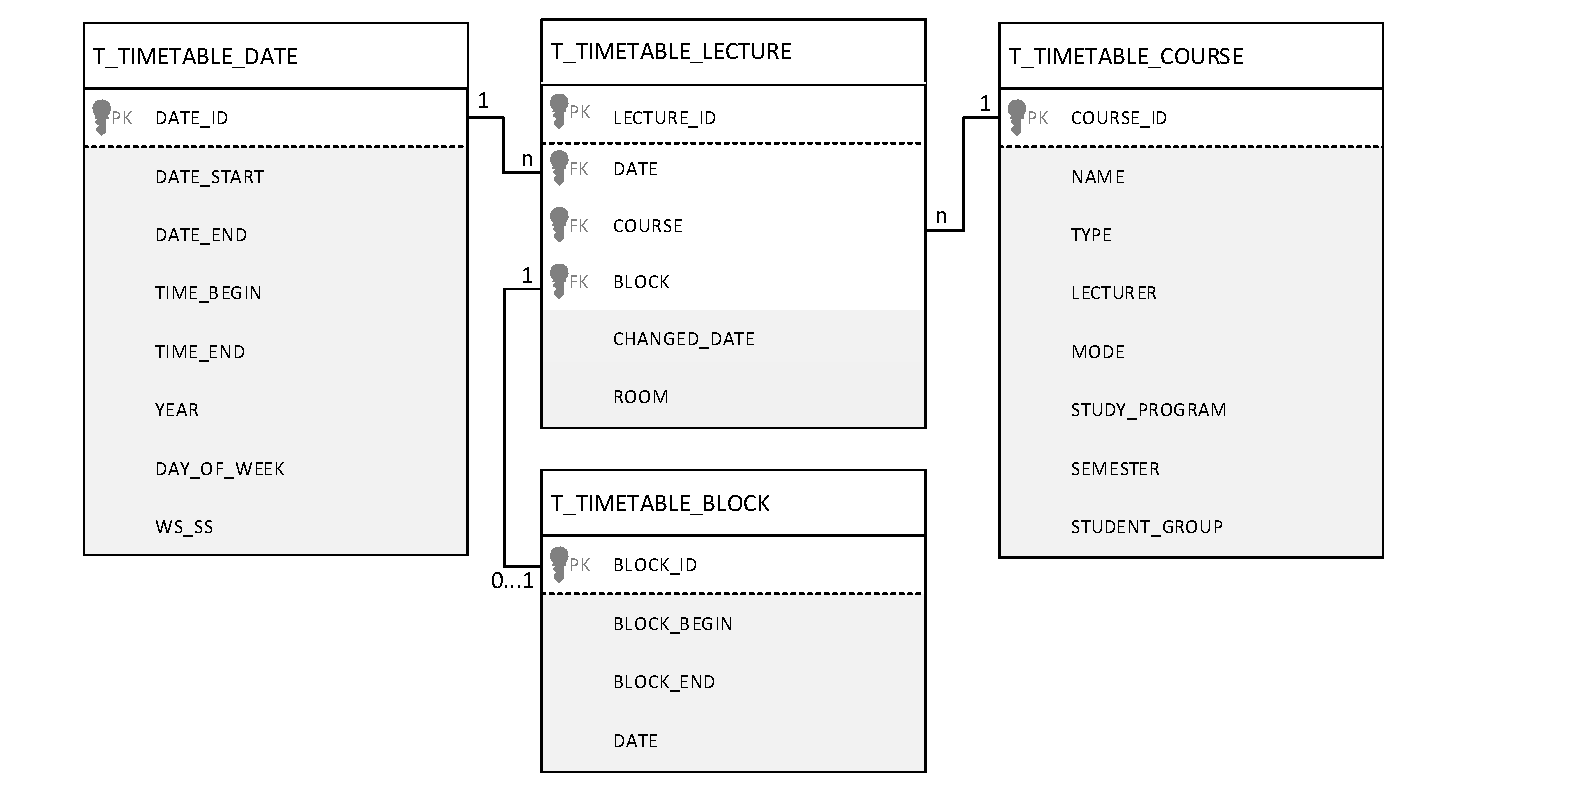
\includegraphics[width=\pictureWidth cm + 3 cm]{Bilder/ER/Timetable_ER.pdf}
\caption{Entity Relation Diagramm der Stundenplan Datenbank\label{fig:timetableER}\protect\footnotemark}
\end{figure}
\footnotetext{Brysiuk, Lehmann (2019)}


% Stundenplanänderung
\section{Planänderungen (Timetable-Change-Service)}
\label{sec:stundenplan}
% Text

Zusätzlich zu der zentralen Aufgabe des allgemeinen und personalisierten Stundenplans muss die Anwendung auch die Änderungen am Stundenplan für den Nutzer zur Verfügung stellen. Dies muss auf verschiedenen Wegen möglich sein. Die Änderungen müssen einerseits frei aufrufbar sein, das heißt, nach einer Anfrage an die Schnittstelle zurückgegeben werden, als neue Änderung aber auch von außen in die Datenquelle eingespeist werden. Um die Benachrichtigung der Clients der Schnittstelle ist dann ein anderer Service zuständig, der seine Informationen jedoch vom Stundenplanänderung-Service bezieht.
\\
\linebreak
Eine normale Anfrage an die vorhandenen Änderungen kann nochmals in zwei Arten unterteilt werden. Einerseits muss die Schnittstelle alle Daten zurückgeben können, die sie enthält, andererseits soll eine Anfrage auch gefilterte Ergebnisse zurückerhalten können. So kann ein registrierter Nutzer beispielsweise alle Änderungen abfragen, die seine Vorlesungen betreffen oder die sein Fachsemester in seinem Studiengang betreffen. 
\\
\linebreak
Die Daten, die die Anwendung auf eine solche Anfrage zurückgibt, muss mindestens folgende Informationen enthalten:

\begin{itemize}

\item Kennzeichnung der Vorlesung (Kann bei der Zuordnung zu einer echten Vorlesung genutzt werden)

\item Art der Änderung (Ausfall, Verschiebung, etc.)

\item Zeitpunkt der Änderung (Datum, Uhrzeit)

\end{itemize}

Anhand dieser Informationen ist nicht nur die allgemeine Vorlesung identifizierbar, sondern auch der Termin, an dem die Änderung eintrifft. Dies ist besonders bei Verschiebungen oder Ausfällen von einzelnen Veranstaltungen wichtig.

% Stundenplanänderung Anforderung
\subsection*{Anforderung an Schnittstelle}
\label{sec:stundenplan_change_anforderung}
% Text

Der Service und die Schnittstelle für die Stundenplanänderungen ist im Vergleich zum Stundenplan Service relativ leichtgewichtig. Hier wird lediglich eine Schnittstelle benötigt, welche die Änderungen bereitstellt. Diese sollten entweder alle ausgegeben oder anhand von Kriterien wie Datum, Studiengang oder ähnlichem gefiltert werden. Zudem soll es möglich sein, neue Änderungen über die \ac{REST}-Schnitt\-stelle hinzuzufügen, da im Hintergrund des Services eine eigene Datenbank stehen soll. Zudem muss der Service den Benachrichtigungsservice über neue Änderungen informieren, sobald er diese erkennt. 

% Stundenplanänderung Umsetzung
\subsection*{Spezifikation der Ressourcen}
\label{sec:stundenplan_change_api}
% Text
In der Ressource \lstinline[columns=fixed]{/changes} und allen Subressourcen außer \lstinline|/{id}| und \lstinline[columns=fixed]{/filters} kann im Body der Filter für das Datum übergeben werden.

\begin{itemize}
\item \subsubsection{GET/POST/DELETE:\\ /changes}
Die Methode GET liefert alle Änderungen unter der Berücksichtigung vom gesetzten Datum. POST erlaubt erstellen von eine oder mehreren Änderungen und DELETE löscht alle Änderungen.
\item \subsubsection{GET/PATCH/DELETE:\\ /changes/\{id\}} 
Die Methode GET liefert eine Änderung für die übergebene \ac{ID}. Mit PATCH kann die Vorlesung Änderung geändert beziehungsweise korrigiert werden und DELETE löscht diese Änderung
\item \subsubsection{GET/POST/DELETE:\\ /changes/program} 
Die Methode GET liefert eine Liste vorhandener Studiengänge. POST erlaubt die Studiengangliste zu erweitern und DELETE löscht die komplette Studiengangliste.
\item \subsubsection{GET/PATCH/DELETE:\\ /changes/program/\{program\}} 
Die Methode GET liefert alle Änderungen die zur gesetzten Studiengang gehören. Mit PATCH kann der Studiengang geändert beziehungsweise korrigiert werden und DELETE löscht diesen Studiengang aus der Studiengangliste.
\item \subsubsection{GET/POST/DELETE:\\ /changes/program/\{program\}/semester} 
Die Methode GET liefert eine Liste vorhandener Semester. POST erlaubt die Semesterliste zu erweitern und DELETE löscht die komplette Semesterliste.
\item \subsubsection{GET/PATCH/DELETE:\\ /changes/program/\{program\}/semester/\{semester\}} 
Die Methode GET liefert alle Änderungen die zu gesetzten Studiengang und Semester gehören. Mit PATCH kann der Semester geändert beziehungsweise korrigiert werden und DELETE löscht diesen Semester aus der Liste.
\item \subsubsection{GET:\\ /changes/filters} 
Liefert alle vorhandenen Filterkriterien, in dem Fall nur das Datum.
\item \subsubsection{GET:\\ /changes/filters/date} 
Liefert die Formatierung für den Filter Datum.
\end{itemize}

% Stundenplanänderung DB
\subsection*{Datenbank Konzept}
\label{sec:stundenplan_change_db}
%Text

Die Stundenplanänderungen liegen, wie die Stundenplaninformationen, ebenfalls bereits auf dem Lehre Server der Hochschule Hof in der Datenbank \textit{huapp_time_\-table}. Dort existiert eine Tabelle, in der die Veranstaltungen, die sich ändern, mit den alten Daten und den neuen Daten abgelegt werden. Jedoch werden diese Änderungen nur mit den Namen der dazugehörigen Vorlesung und den zeitlichen Daten der ursprünglichen Veranstaltung hinterlegt. Es wurde kein Fremdschlüssel genutzt, um die Vorlesung, die betroffen ist, mit der Änderung zu verknüpfen. Somit sind die Daten für das menschliche Auge durchaus lesbar, für Maschinen aber nur schwer zu verarbeiten.
\\
\linebreak
Deshalb wird auch hierfür eine eigene Datenbank genutzt, welche die eingehenden Einträge mit den vorhandenen Vorlesungen abgleicht und mit der passenden Vorlesungs-ID referenziert. Somit kann jede Änderung auch einer einzigen Veranstaltung zugeordnet werden. Dies erfordert jedoch einen externen Service, welcher die Tabellen der originalen Datenbank miteinander Vergleicht und daraus die Einträge für die neue Datenbank generiert. 

\begin{figure}[H]
\centering
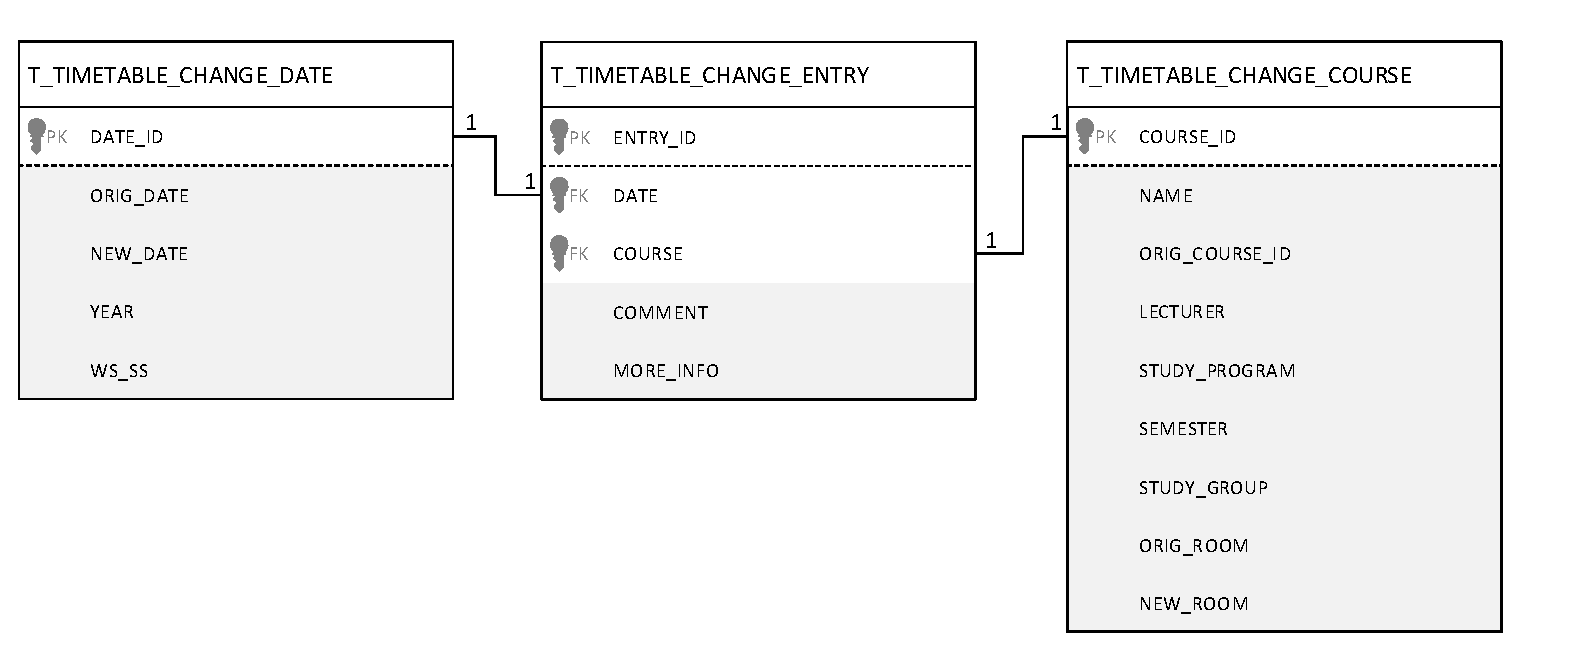
\includegraphics[width=\pictureWidth cm + 2.5 cm]{Bilder/ER/TimeTableChange_ER.pdf}
\caption{Entity Relation Diagramm der Datenbank zu den Planänderungen\label{fig:timetableER}\protect\footnotemark}
\end{figure}
\footnotetext{Brysiuk, Lehmann (2019)}

% Mensa
\section{Speiseplan (Mensa-Service)}
\label{sec:mensa}
% Text
Bei der Wahl der Ernährung spielen soziale, politische, ökonomische, psychologische und kulturelle Dimensionen eine Rolle. Somit macht die Ernährung mehr als nur den Körper mit Nährstoffen zu versorgen. 
%Referenz: https://www.dge.de/presse/pm/der-mensch-ist-was-er-isst-1/
Das Ziel ist es, den Studierenden die Möglichkeit zur Verfügung stellen, ihren Speiseplan individuell nach ihren Bedürfnissen anzupassen. Dies wird durch den Mensa-Service realisiert. Der Service stellt dem Client alle Informationen über Gerichte zur Verfügung und erlaubt auch diese gezielt zu sortieren und zu personalisieren.

% Mensa Anforderung
\subsection*{Anforderung an Schnittstelle}
\label{sec:mensa_anforderung}
% Text
Eine Schnittstelle für die Speiseplan Daten steht derzeit nicht zur Verfügung. Die Informationen für den Speiseplan, die für die Hochschul-App benötigt werden, werden auf der Webseite des Studentenwerk-Oberfranken im Navigationsmenü Speiseplan für die Standorte Hof und Münchberg zur Verfügung gestellt. Der Ausschnitt der Webseite für den Speiseplan aus Abbildung \ref{fig:swo_speiseplan} lässt sich in 7 Bereiche kategorisieren:

\begin{figure}[H]
\centering
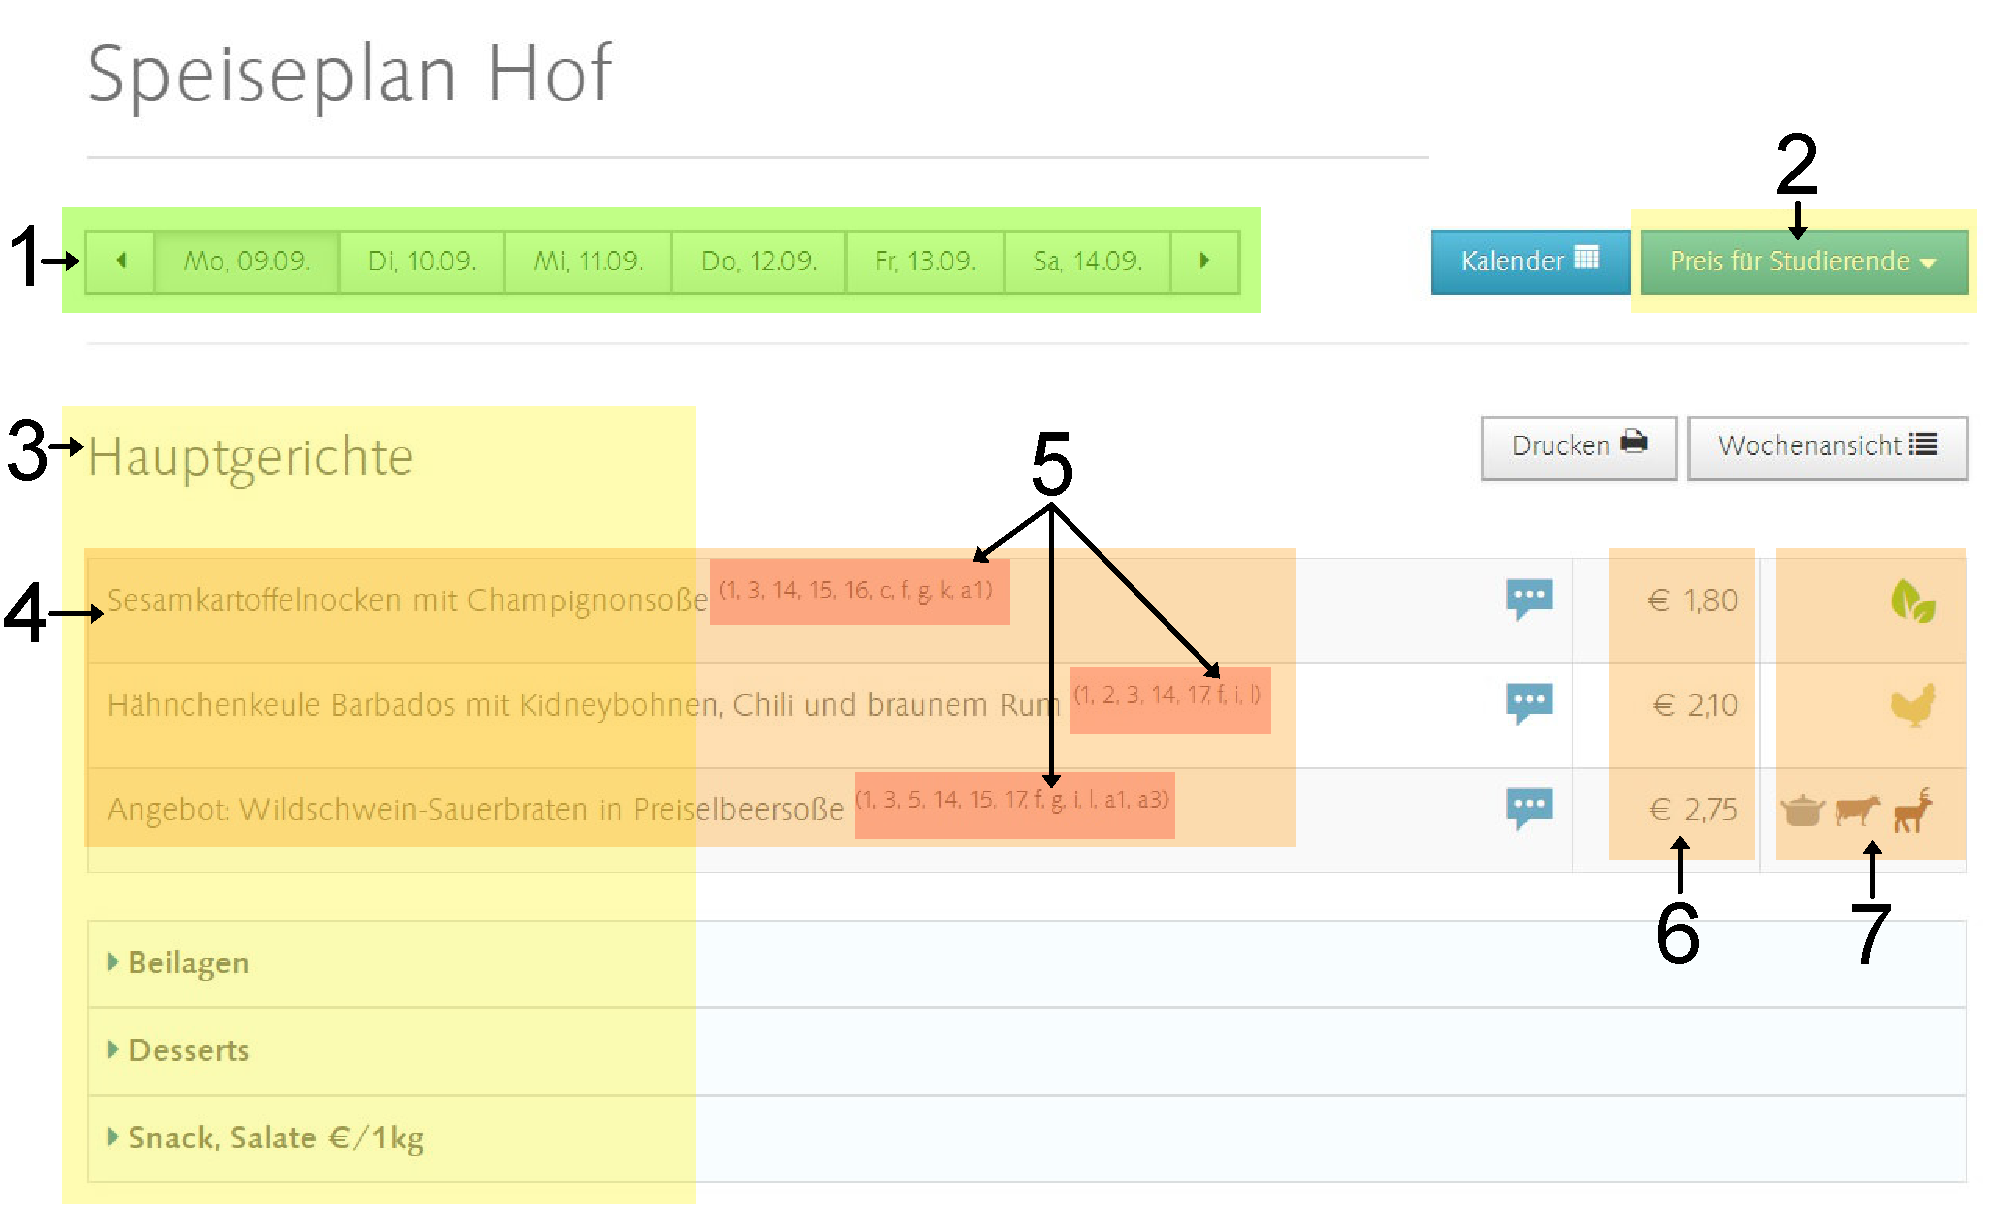
\includegraphics[width=\pictureWidth cm + 2cm]{Bilder/Sonstiges/Speiseplan_Infoblock.pdf}
\caption{Speiseplan Informationsblöcke\label{fig:swo_speiseplan}\protect\footnotemark}
\end{figure}
\footnotetext{Brysiuk, Lehmann (2019)}


\begin{enumerate}
\item Datum für Speiseplan
\item Preistyp für alle Gerichte
\item Kategorie des Gerichts
\item Bezeichnung des Gerichts
\item Zusatzstoffe/ Inhaltsstoffe/ Allergien des Gerichts
\item Preis des Gerichts
\item Kennzeichnung des Gerichts
\end{enumerate}

Wobei sich diese sieben Blöcke in drei weitere übergeordnete Bereiche einordnen lassen. Der erste bezieht sich auf die zeitliche Darstellung des Speiseplans. Der Speiseplan muss für ein beliebiges Datum oder einen Zeitraum dargestellt werden können. Der zweite bezieht sich auf die Darstellung und den Umfang des Speiseplans, bei dem der Preistyp und die Kategorie der Gerichte eine Rolle spielt. Also muss der Speiseplan zusätzlich zu den zeitlichen Einstellungen die Gerichte nach Preistyp und Kategorie sortiert werden können. Der dritte Block bezieht sich auf ein spezifisches Gericht, bei dem Bezeichnung, Zusatzstoffe/ Inhaltsstoffe/ Allergene, Kennzeichnung und der Preis des Gerichts eine Rolle spielen. Durch die Abbildung \ref{fig:analysemensa} wird dargestellt, nach welchen Faktoren der Speiseplan sortiert und personalisiert werden kann. Es muss aber beachtet werden, dass das Backend nur für Kategorisierung und Filterung der einzelnen Gerichten zuständig ist und das Frontend für die Implementierung der Suche.

\begin{figure}[H]
\centering
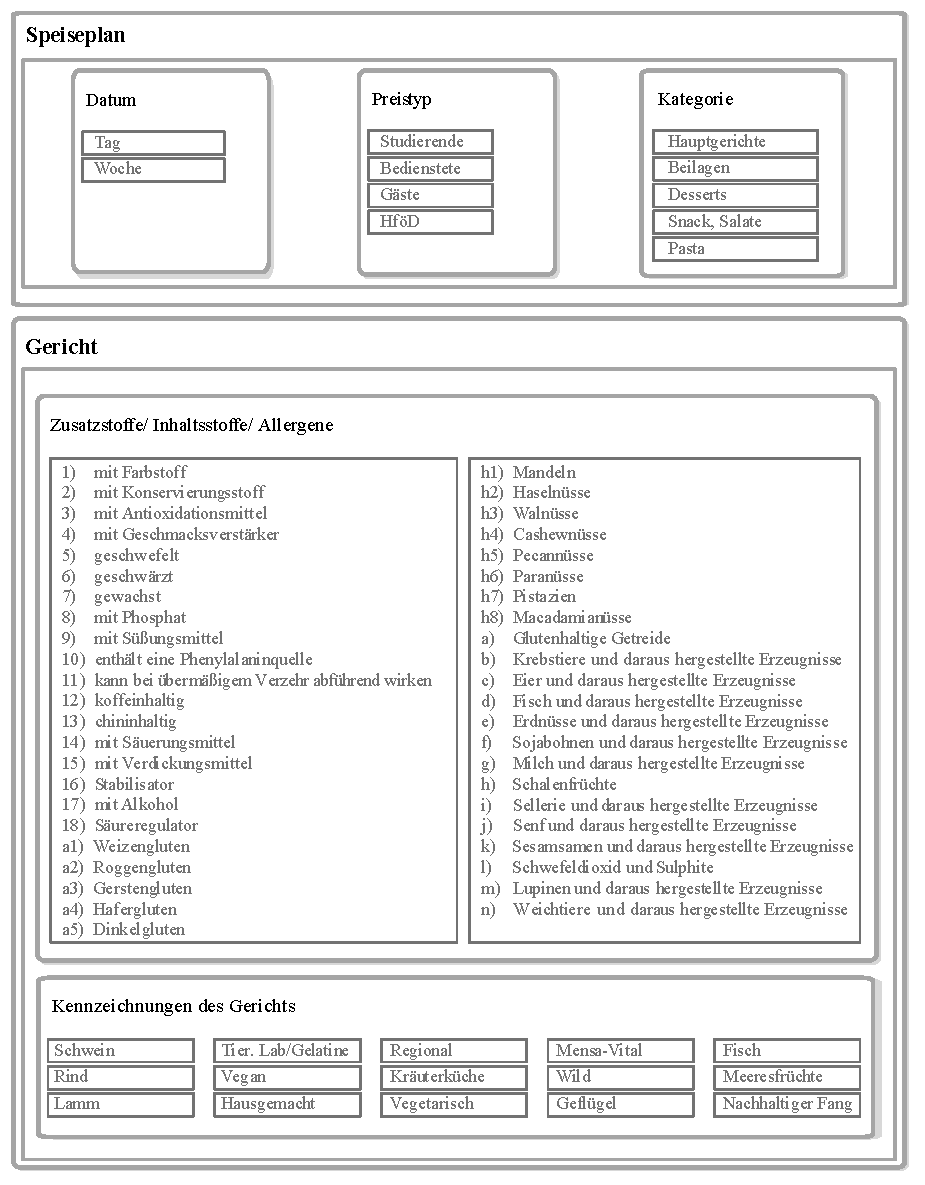
\includegraphics[width=\pictureWidth cm + 2 cm]{Bilder/Sonstiges/Speiseplan_Kategorisierung.pdf}
\caption{Bereiche der Speiseplaninformationen\label{fig:analysemensa}\protect\footnotemark}
\end{figure}\footnotetext{Brysiuk, Lehmann (2019)}




Solange keine Schnittstelle für den Speiseplan zur Verfügung steht, wird ein externer Service erstellt, der die Speiseplan Daten von der Webseite des Stundenwerk-Oberfranken ausliest und in eine Datenbank abspeichert.

% Mensa Umsetzung
\subsection*{Spezifikation der Ressourcen}
\label{sec:mensa_api}
Bezogen auf die technischen Anforderungen aus dem Kapitel \ref{sec:mensa_anforderung} und der Kategorisierung des Speiseplans, werden hier die notwendigen Ressourcen für den Mensa-Service spezifiziert.
\\
\linebreak
Alle GET-Methoden - außer die Subressourcen /filters und /\{id\} - können im Body die Filter für Preis, Kategorie, Kennzeichnung und Zusatzstoffe/Inhaltsstoffe/Allergie der Gerichte entgegen nehmen. Es müssen nicht alle Filter gesetzt werden. Ohne Übergabe der Filter werden standardmäßig alle Gerichte zurückgegeben. Wird der Filter Preistyp gesetzt, so werden nur die Gerichte mit diesem Preistyp zurückgegeben, sonst werden alle Preistypen zurückgegeben. In Kategorie, Zusatzstoffe oder Kennzeichnung des Gerichts können ein oder mehrere Filtertypen festgelegt werden. Wobei die übergebenden Filtertypen für Kategorie und Kennzeichnungen in den Gerichten enthalten sind und die Zusatzstoffe/Inhaltsstoffe/Allergene nicht. 
\begin{itemize}
\item \subsubsection*{GET/POST/DELETE:\\ /menu} 
Die Methode GET liefert alle Gerichte unter der Berücksichtigung von gesetzten Filtern. POST erlaubt erstellen von ein oder mehreren Gerichten und DELETE löscht alle Gerichte. 
\item \subsubsection*{GET/PATCH/DELETE:\\ /menu/\{id\}} 
Die Methode GET liefert ein Gericht für die übergebene ID. Mit PATCH kann das Gericht geändert beziehungsweise korrigiert werden und DELETE löscht dieses Gericht.
\newpage
\item \subsubsection*{GET:\\ /menu/filters} 
Liefert alle Kategorien, Legenden, Zusatzstoffe und Preistypen die vorhanden sind.
\item \subsubsection*{GET/POST/DELETE:\\ /menu/filters/categories} 
Die Methode GET liefert alle möglichen Kategorien. Mit POST können ein oder mehrere neue Kategorien eingefügt werden und DELETE löscht alle verfügbaren Kategorien.
\item \subsubsection*{GET/PATCH/DELETE:\\ /menu/filters/categories/\{id\}} 
Die Methode GET liefert Informationen zur der übergebene Kategorien ID. Mit PATCH kann die Kategorie geändert beziehungsweise korrigiert werden und DELETE löscht diese Kategorie.
\item \subsubsection*{GET/POST/DELETE:\\ /menu/filters/labels} 
Die Methode GET liefert alle möglichen Kennzeichnungen zu den Gerichten. Mit POST können ein oder mehrere neue Kennzeichnungen eingefügt werden und DELETE löscht alle verfügbaren Kennzeichnungen.
\item \subsubsection*{GET/PATCH/DELETE:\\ /menu/filters/labels/\{id\}} 
Die Methode GET liefert Informationen zur der übergebene Kennzeichnung ID. Mit PATCH kann die Kennzeichnung geändert beziehungsweise korrigiert werden und DELETE löscht diese Kennzeichnung.
\newpage
\item \subsubsection*{GET/POST/DELETE:\\ /menu/filters/excludes} 
Die Methode GET liefert alle verfügbaren Zusatzstoffe/Inhaltsstoffe/Allergie. Mit POST können ein oder mehrere neue Zusatzstoffe/Inhaltsstoffe/Allergie eingefügt werden und DELETE löscht alle verfügbaren Zusatzstoffe/Inhaltsstoffe/Allergie. 
\item \subsubsection*{GET/PATCH/DELETE:\\ /menu/filters/excludes/\{id\}} 
Die Methode GET liefert Informationen zur der übergebenen Zusatzstoffe/Inhaltsstoffe/Allergie ID. Mit PATCH kann der Zusatzstoff/Inhaltsstoff/Allergie geändert beziehungsweise korrigiert werden und DELETE löscht diesen Zusatzstoff/Inhaltsstoff/Allergie.
\item \subsubsection*{GET:\\ /menu/filters/prices} 
Die Methode GET liefert alle verfügbaren Preistypen.
\item \subsubsection*{GET:\\ /menu/week} 
Liefert alle Gerichte unter der Berücksichtigung von gesetzten Filtern für die aktuelle Woche.
\item \subsubsection*{GET:\\ /menu/week/\{week\}} 
Liefert alle Gerichte unter der Berücksichtigung von gesetzten Filtern für die übergebene Woche.
\item \subsubsection*{GET:\\ /menu/week/\{week\}/\{day\}} 
Liefert alle Gerichte unter der Berücksichtigung von gesetzten Filtern für den übergebenen Wochentag in der übergebenen Woche.
\item \subsubsection*{GET:\\ /menu/week/\{week\}/\{day\}/\{until-day\}} 
Liefert alle Gerichte unter der Berücksichtigung von gesetzten Filtern für die Zeitspanne innerhalb der übergebenen Wochentagen (inklusiv) in der übergebenen Woche.
\item \subsubsection*{GET:\\ /menu/date} 
Liefert alle Gerichte unter der Berücksichtigung von gesetzten Filtern für den heutigen Tag.
\item \subsubsection*{GET:\\ /menu/date/\{date\}} 
Liefert alle Gerichte unter der Berücksichtigung von gesetzten Filtern für den übergebenden Datum.
\item \subsubsection*{GET:\\ /menu/date/\{date\}/\{until-date\}} 
Liefert alle Gerichte unter der Berücksichtigung von gesetzten Filtern für die Zeitspanne zwischen übergebenen Datumsangaben (inklusiv).
\end{itemize}

% Mensa DB
\subsection*{Datenbank Konzept}
\label{sec:mensa_db}
%Text

Um eine performante und anpassbare Datenquelle für die Daten des Speiseplans des Studentenwerk Oberfrankens zu haben, wird auch hierfür eine Datenbank erstellt. Da sich die Daten kaum ändern entlastet dies auch die Schnittstelle, von der letztendlich die Daten ausgelesen werden. Für die Funktionen des Mensa Services werden lediglich die Gerichte an sich benötigt. Diese Gerichte brauchen folgende Informationen:

\begin{itemize}
\item \textbf{ID} 
\\Einen klaren Identifier für ein Gericht, um für dieses Gericht weitere Informationen abfragen zu können
\item \textbf{Datum} 
\\Das Datum, an dem das Gericht angeboten wird
\item \textbf{Kategorie} 
\\Die Art von Gericht, zu dem der Eintrag zugeteilt werden kann
\item \textbf{Beschreibung} 
\\Eine Kurzbeschreibung für das Gericht
\item \textbf{Zugeordnete Kennzeichnungen} 
\\Kennzeichnungen, die das Gericht beschreiben
\item \textbf{Preis für alle Preistypen} 
\\Verschiedene Preise für verschiedene Gästegruppen
\item \textbf{Enthaltene Zusatzstoffe/Inhaltsstoffe/Allergene} 
\\Hinweise zum Inhalt und für Allergiker
\end{itemize}

Das resultierende \ac{ER}-Diagramm in Abbildung \ref{fig:ermensa} zeigt die einfache Struktur der Datenbank für den Mensa Service. Für die Zusatzstoffe und die Kennzeichner der Gerichte werden sogenannte \textit{n zu n} Beziehungen benötigt, für alles andere reichen Fremdschlüssel zur Zuordnung der weiteren Informationen. Die Tabelle \textit{T_MENU_PRIZE} ähnelt zudem einer Dimensionstabelle eines Data Warehouses, statt die Preise anhand eines Standardwertes berechnen zu müssen, werden alle möglichen Kombinationen abgelegt und können dementsprechend ausgelesen werden. Es bietet sich ebenfalls an, einen \textit{Non-Clustered}-Index auf die Fremdschlüssel zur Tabelle \textit{T_MENU\-_CATEGORY_TYPE} in der Spalte \textit{CATEGORY} der Tabelle \textit{T_MENU_DISH} anzulegen. Des weiteren ist ein weiterer \textit{Non-Clustered}-Index auf der Spalte \textit{DATE} der selben Tabelle sinnvoll. Diese beiden Werte sind die, nach denen am wahrscheinlichsten sortiert und gefiltert wird. Im späteren Betrieb der Datenbank könnte man auch noch testen, ob sich einer der beiden Indizes als \textit{Clustered}-Index eignen würde, da eine dauerhafte Sortierung der Einträge der Tabelle \textit{T_MENU_DISH} nach der \textit{ID} nicht zwingend hilfreich ist.

\begin{figure}[H]
\centering
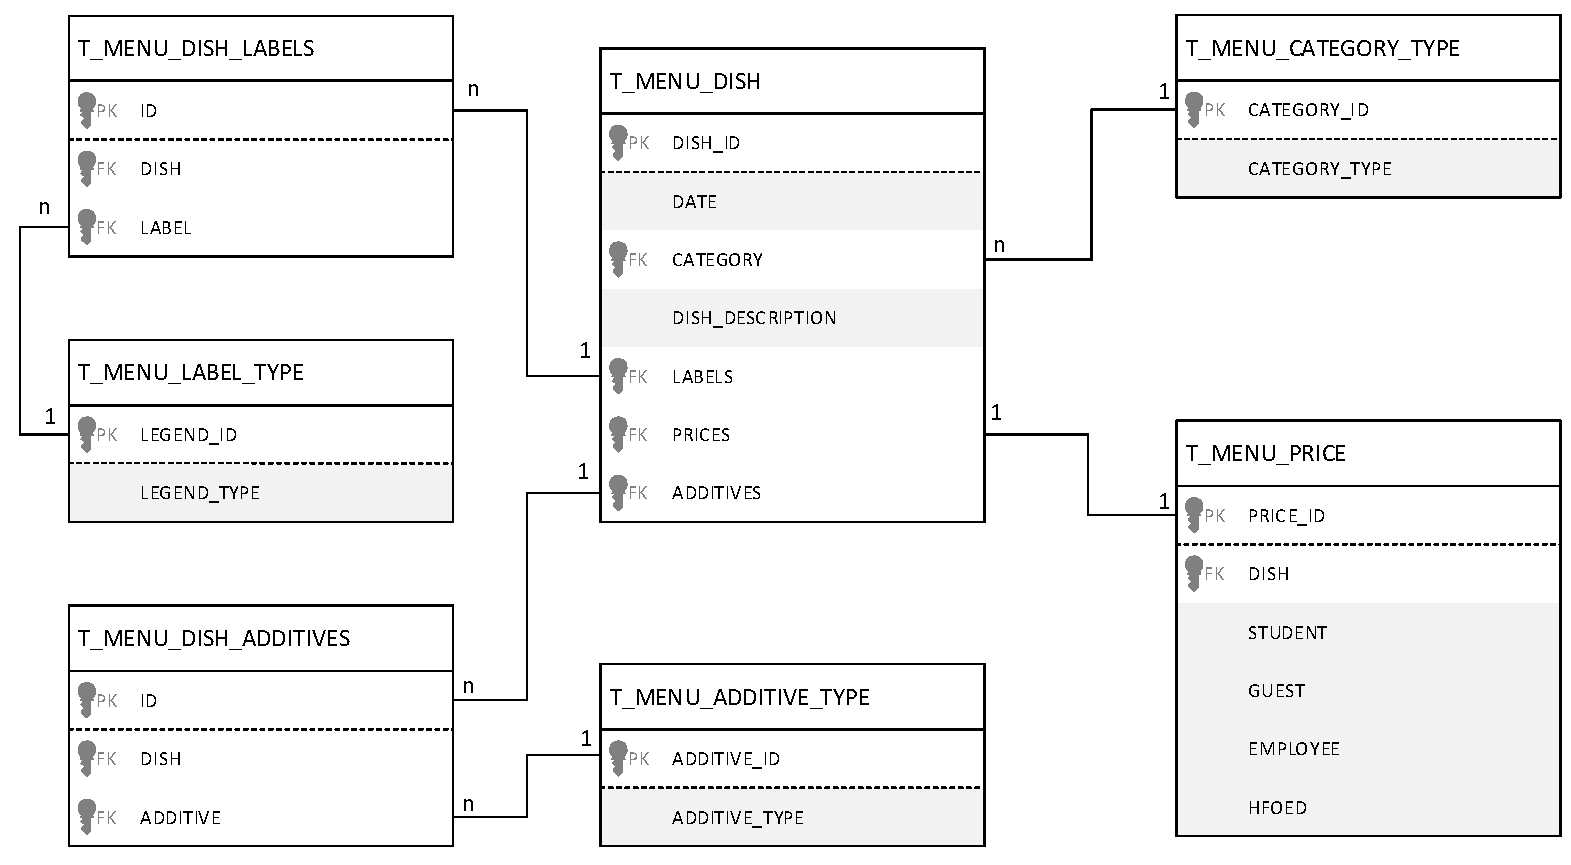
\includegraphics[width=\pictureWidth cm + 2cm]{Bilder/ER/Menu_ER.pdf}
\caption{Entity Relation Digramm des Mensa-Speiseplans\label{fig:ermensa}\protect\footnotemark}
\end{figure}
\footnotetext{Brysiuk, Lehmann (2019)}

Weiterhin zu bemerken ist, dass die Datenbank auf Dauer nur die Gerichte der aktuellen und der nächsten Woche, also im Zeitraum von zwei Wochen, speichern wird. Ein automatisierter Scheduler Job im Mensa Service wird die alten Einträge automatisiert löschen und neue Einträge einspeisen. Für das Löschen der alten Einträge bietet es sich eventuell auch an, einen Datenbank Job zu schreiben, das kann in der Entwicklungsphase getestet werden. Jedoch richtet sich diese Datenbank stark nach dem \ac{KISS} Prinzip, weshalb auch auf komplexere Strukturen verzichtet wurde. Das lässt sich dadurch begründen, dass nur Einträge für den Zeitraum von zwei Wochen gespeichert werden und keine historischen Daten gespeichert werden. Außerdem ist auch eine Änderung in den Formaten der eigentlichen Datenquelle nicht vorhersehbar. Die eigene Tabelle für die Spalte \textit{CATEGORY} der Haupttabelle \textit{T_MENU_DISH} beinhaltet auch eine Beschreibung der einzelnen Einträge, weshalb ein einfacher \textit{Enumeration Type} für diesen Wert keinen Sinn ergibt.


% Notification
\section{Benachrichtigungen (Notification-Service)}
\label{sec:notification}
% Text
Fast in jeder Anwendung sind Push-Notifications eingebunden. Am häufigsten kennt man es von Facebook oder dem Whats-App Messenger, dass die Nachrichten in Echtzeit übertragen werden und direkt auf den Smartphone als Benachrichtigung angezeigt werden. Die Funktionsweise ist einfach, man erhält Benachrichtigungen von einer Programm ohne diese öffnen zu müssen. Dies ermöglichtes, den Benutzer über wichtige Ereignisse oder Neuigkeiten zur informieren ohne die Anwendung zu starten oder diese neu zu laden. Solche Benachrichtigung können für die Studierenden von Vorteil sein. Sollte sich eine Vorlesung ändern oder ausfallen, werden die an der Vorlesung teilnehmenden Studierenden informiert. Aber auch andere Services können von dieser Technik profitieren, wie beispielsweise der Mensa-Service oder der Sprachzentrum-Service. Das Ziel ist es, ein Notification-Service zu erstellen, der eine einheitliche Schnittstelle für alle anderen Services zur Verfügung stellt, um die betroffenen Benutzer über eine Änderung jeglicher Art zu informieren.

\begin{figure}[H]
\centering
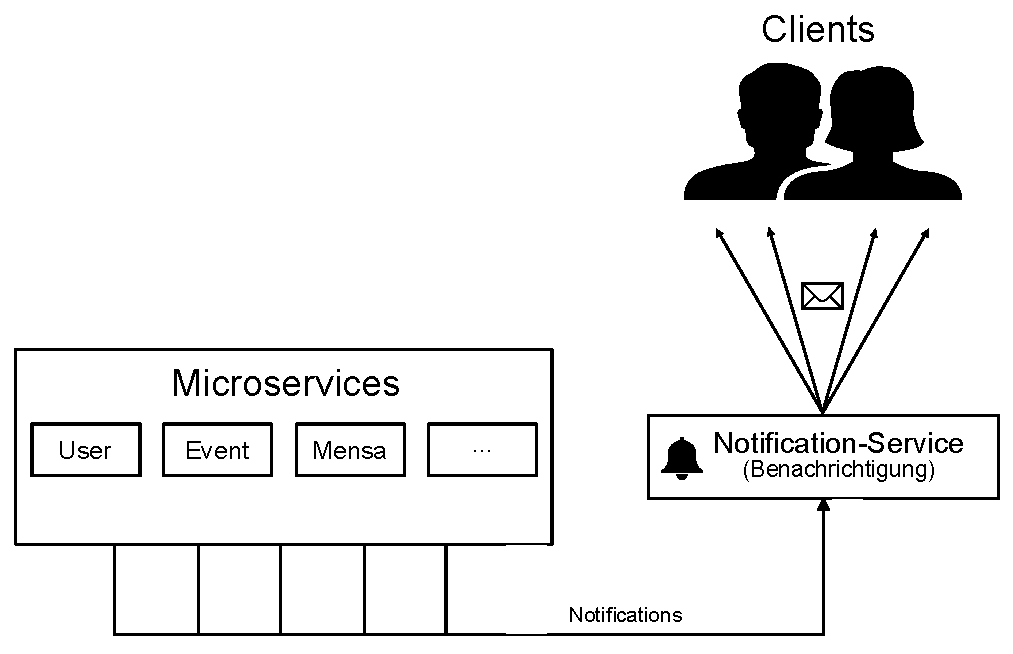
\includegraphics[width=\pictureWidth cm]{Bilder/Prototyp/Notification_Service_Prototype.pdf}
\caption{Benachrichtigungsservice\label{fig:notificationservice}\protect\footnotemark}
\end{figure}
\footnotetext{Brysiuk, Lehmann (2019)}


% Benachrichtigung Anforderung
\subsection*{Anforderung an Schnittstelle}
\label{sec:notification_anforderung}
% Text
Die Funktionalität eines Services, der den Notification-Service in Anspruch nimmt, darf nicht vom Ergebnis des Services beeinflusst werden. Sobald ein Service eine Benachrichtigung an den Notification-Service übermittelt, ist es dem Service nicht mehr wichtig wie, wann und ob die Nachricht zugestellt wird. Damit wird die Abhängigkeit zwischen unterschiedlichen Funktionalitäten reduziert und es wird ein Maß an loser Kopplung garantiert.

\begin{figure}[H]
\centering
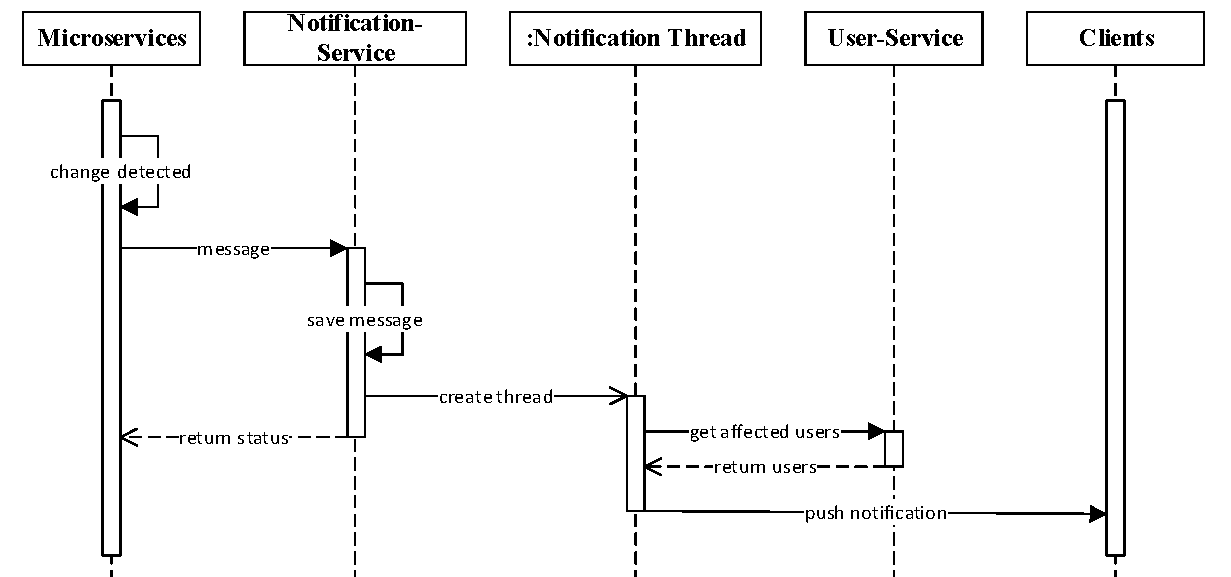
\includegraphics[width=\pictureWidth cm + 2 cm]{Bilder/Sequenz_Diagramm/Notification_Sequenz.pdf}
\caption{Sequenzdiagramm zum Ablauf einer Benachrichtigung\label{fig:notificationsequenz}\protect\footnotemark}
\end{figure}
\footnotetext{Brysiuk, Lehmann (2019)}

In Abbildung \ref{fig:notificationsequenz} ist ein Sequenz Diagramm zu sehen das einen groben Ablauf darstellt, wie eine Benachrichtigung von einem Microservice bis zum Benutzer kommuniziert wird. Der Microservice sendet die Nachricht an den Notification-Service und endet der Prozess für den Microservice. Der \textit{return status} wird vom Microservice ignoriert, sowohl bei einer erfolgreichen Antwort als auch bei einer nicht erfolgreichen Antwort. Der \textit{return status} wurde im Sequenz Diagramm nur aufgenommen, weil eine \ac{REST}-\ac{API} immer eine Antwort zurück senden muss. Ab jetzt ist nur der Notification-Service zuständig für eine erfolgreiche Übermittlung der Nachricht an die Clients. Um sicher zu gehen, dass die Nachricht nicht auf dem Weg verloren geht, bei ersten Versuch nicht erfolgreich an den Client übermittelt werden kann oder beim Absturz des Services verloren geht, wird die Nachricht zuerst in der Datenbank abgelegt. Der Notification-Service ist selbständig verantwortlich dafür, die jeweiligen Benutzer für die Nachricht zu finden und zu informieren. 

% Benachrichtigung API
\subsection*{Spezifikation der Ressourcen}
\label{sec:notification_api}
Der Notification-Service benötigt im Grunde zwei Ressourcen, die eine zur Registrierung eines Clients, die andere für die Übergabe einer Nachricht. Um den Service leichter mit den Hochschul-\ac{App} Services nutzen zu können, wurde der Service um die Subressourcen \textit{/lectures} und \textit{/mensa} erweitert. Außerdem wurde die Benachrichtigung einzelner Benutzer berücksichtigt. Die Übergabe der Informationen an den Notification-Service erfolgt im Body Bereich. 
\begin{itemize}
\item \subsubsection{POST: \\/register} 
Für die Registrierung des Clients, der über Neuigkeiten informiert werden soll.
\item \subsubsection{POST: \\/message} 
Benachrichtigung an alle Benutzer des registrierten Clients.
\item \subsubsection{POST: \\/message/\{userId\}} 
Benachrichtigung an übergebenen Benutzer.
\item \subsubsection{POST: \\/message/lectures} 
Benachrichtigung an Benutzer, die für die Vorlesung hinterlegt sind.
\item \subsubsection{POST: \\/message/mensa} 
Benachrichtigung an Benutzer, die für ein Gericht hinterlegt sind.
\end{itemize}

% Notification DB
\subsection*{Datenbank Konzept}
\label{sec:notification_db}
Wie bereits vorher erwähnt wurde, werden die Nachrichten temporär in der Datenbank abgespeichert und solange behalten, bis die Benachrichtigung tatsächlich die Benutzer erreicht hat. Durch die Spezifikation der Ressourcen ergeben sich folgende Tabellen.

\begin{enumerate}
\item Abspeicherung der Registrierten Clients
\item Benachrichtigung und zugehörige Informationen
\end{enumerate}


\begin{figure}[H]
\centering
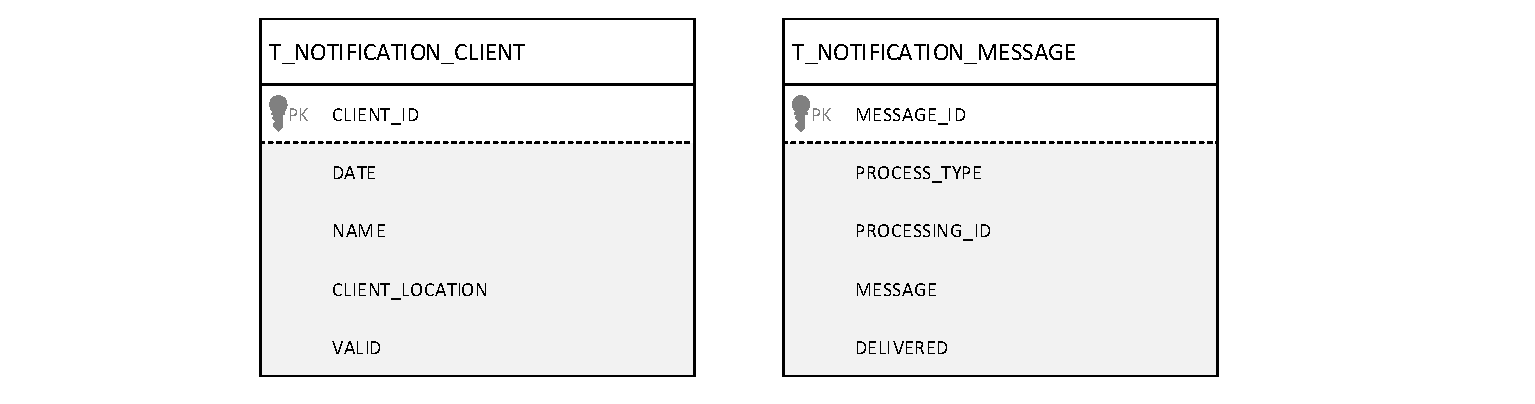
\includegraphics[width=\pictureWidth cm + 3 cm]{Bilder/ER/Notification_ER.pdf}
\caption{Entity Relation Diagramm der Benachrichtigungs Datenbank\label{fig:notificationER}\protect\footnotemark}
\end{figure}
\footnotetext{Brysiuk, Lehmann (2019)}


% Auth
\section{Sicherheit (Auth-Service)}
\label{sec:auth}
% Text
Um alle Services abzusichern, wird ein Sicherheitskonzept benötigt. Zum einen müssen die Clients autorisiert werden und anderen die Benutzer authentifiziert werden. Um einen gesicherten Zugriff auf die Microservices zu gewährleisten, ohne dass die Services vom Authentifizierung-Service abhängig sind, wird ein Token an die Microservices übersendet, über welchen die Zugriffserlaubnis von jeden Service unabhängig geprüft werden kann, ohne den Authentifizierung Service aufzurufen.

\begin{figure}[H]
\centering
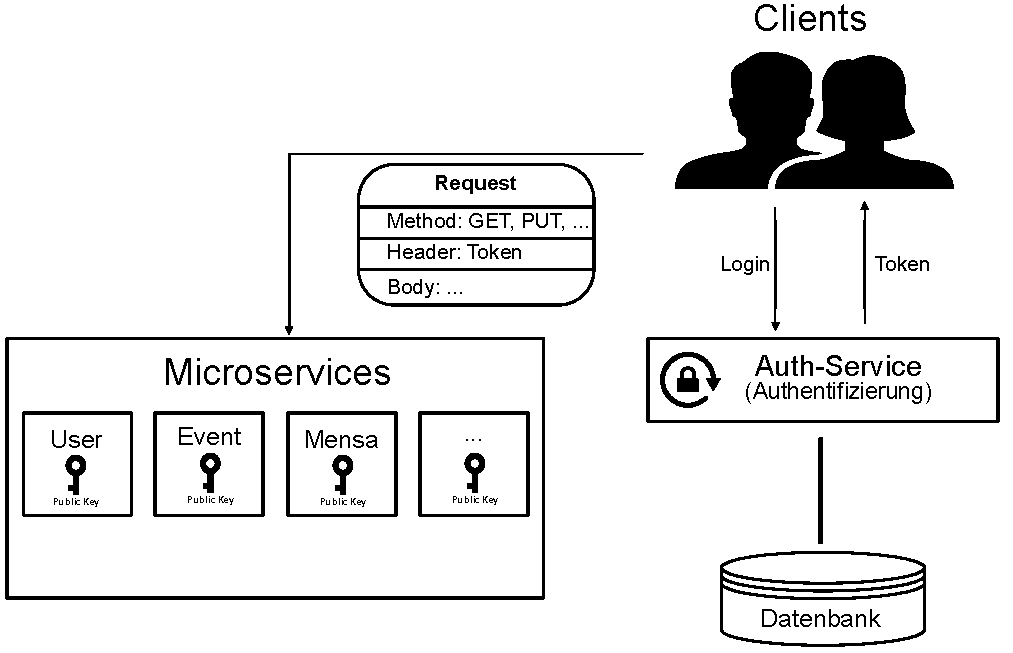
\includegraphics[width=\pictureWidth cm]{Bilder/Prototyp/Auth_Service_Prototype.pdf}
\caption{Authentifizierungsservice\label{fig:authservice}\protect\footnotemark}
\end{figure}
\footnotetext{ebd.}

Für die Zugriffssteuerung wird das Konzept von Rollen und Rechten verwendet. Ausführliche Behandlung diesen Services ist in der hierzu parallel angefertigten Bachelorarbeit zu sehen\autocite[Vgl.][]{andreasba}.

% user
\section{Anwenderverwaltung (User-Service)}
\label{sec:user}
%Text
Der User-Service dient dazu, Benutzer zu verwalten und das mitsamt ihrer Accountinformationen und Einstellungen. Die ausführliche Behandlung dieses Services ist in der hierzu parallel angefertigten Bachelorarbeit zu sehen\footnote{ebd.}.

% Futher Information
\section{Weitere Dienste}
\label{sec:ausblick}
%Text
Die Services Sprachzentrum und Termine sind zwar in der Architektur der Hoch\-schul-\ac{App} berücksichtigt worden, jedoch überschreiten diese den Umfang dieser Bachelorarbeit. Durch die modularisierte und flexible Architektur können diese Services jederzeit separat entwickelt werden und an die aus dieser Arbeit entstandene Hoch\-schul-\ac{App} verknüpft werden.


% Ausblick Fazit
\chapter{Ausblick und Fazit}
\label{sec:ausblick_fazit}

Im Zuge der Digitalisierung werden die Anforderungen an moderne \acp{App} immer höher. Zum einen muss die Anwendung benutzerfreundlich gestaltet sein, zum anderen immer den neuesten Entwicklungen folgen, die es im Bereich der Smartphones gibt. So muss man sich im Laufe der Entwicklung eines neuen Produktes oft entscheiden, ob man eine leichtgewichtige Anwendung schafft, die nur die Kernfunktionen übernimmt, für die sie ursprünglich gedacht wurde, oder ob die Entwicklung breiter ausfällt und man eine Anwendung schafft, die dem Nutzer mehr abnimmt, als nur die Kernfunktionen. Dabei muss am Anfang der Erarbeitung des Konzeptes immer der Grundsatz stehen, das Programm so aufzubauen, dass man im Entwicklungsprozess alle Möglichkeiten offen hat und genau das ist es, was das große Ziel dieser Arbeit ist. Eine Anwendung zu entwerfen, die anfangs die wichtigsten Grundlagen bereitstellt, die aber im Laufe der Zeit immer weiter entwickelt und erweitert werden kann.
\\
\linebreak
Der Fokus auf modulare und erweiterbare Anwendungen steht aktuell im Mittelpunkt der modernen Softwareentwicklung, deshalb sollte auch das das Ziel eines Projektes sein, das in einer Hochschule von Studierenden bearbeitet wird, die später mit bestem und modernstem Wissen in die Arbeitswelt einsteigen sollen. In den vorhergehenden Kapiteln dieser Arbeit wird mehrmals der Grundsatz der Erweiterbarkeit bei einer Microservice Architektur erwähnt und erläutert. Genau nach diesem Grundsatz wird die Hochschul-\ac{App} auch aufgebaut sein, das heißt, dass es in Zukunft die Möglichkeit geben wird, die Funktionen der Anwendung zu erweitern. Dieses Kapitel soll nun kurz beleuchten, welche weiteren Features noch möglich und sinnvoll sind.

\section{Ausblick\label{sec:ausblick}}

Einige der funktionalen Anforderungen aus den Kapiteln \ref{sec:anforderungen_ag}, \ref{sec:anforderungen_io} und \ref{sec:anforderungen_sz}, wurden in dieser Arbeit nicht weiter betrachtet. Wie bereits erwähnt, stellt die gewählte Architektur des Projektes die Möglichkeit dar, weitere Funktionen einzubinden, ohne etwas am bestehenden Programmcode ändern zu müssen. Die in dieser Bachelorarbeit nicht betrachteten möglichen Funktionen werden im folgenden aufgelistet.

\subsection*{Sprachumfang}

Im Rahmen der Internationalisierungsbemühungen der Hochschule Hof liegt es im Interesse des International Office, eine Hochschul-\ac{App} anbieten zu können, die in mehreren Sprachen erhältlich ist. Einige mögliche Vorschläge und favorisierte Sprachen der aktuellen Studierenden der Hochschule Hof wurden in Kapitel \ref{sec:anf_io} bereits aufgelistet. Zusätzlich zu den bereits im Funktionsumfang dieser Bachelorarbeit und der zugehörigen Praxisarbeit \footnote{Siehe Kapitel \ref{sec:nebenlektuere}} enthaltenen Sprachen Deutsch und Englisch kann die Anwendung ebenfalls um weitere Sprachen erweitert werden. Dazu könnte ein Konzept erstellt werden, das eine kontinuierliche Einbindung neuer Sprachen unterstützt. So könnten internationale Studierende schnell eigene Sprachen einpflegen. 

\subsection*{Verlinkung wichtiger Informationen}

Ein Wunsch, der aus den Umfragen in Kapitel \ref{sec:umfrage_erg} hervorgeht, ist die Verlinkung wichtiger Informationen zu den Vorlesungen, die im Stundenplan aus der Schnittstelle ausgelesen werden. Dazu gehören beispielsweise eine Referenz auf das entsprechende Modulhandbuch der Vorlesung oder auch die in Kapitel \ref{sec:anf_sz} erwähnten Anmeldungen zu den Sprachkursen. Diese Informationen sind in den vorhandenen Datenbanken der Hochschule nicht vorhanden, somit muss erst analysiert werden, wie man die passenden Informationen zu den Vorlesungen zuteilen kann.

\subsection*{Sprachkursinformationen}

Anders als nur die Verlinkung der Anmeldung zu den Sprachkursen verhält es sich mit den allgemeinen Informationen zu den Sprachkursen. Ein Sprachkurs an sich enthält weit mehr Informationen, als es normale Vorlesungen tun. Ein Sprachkurs hat vorausgesetzte Kenntnisse oder vorhergehende Sprachkurse, die erst abgelegt werden müssen, um teilnehmen zu dürfen. Zudem bieten viele Sprachkurse ebenfalls eine Zertifizierung an, welche am Ende des Kurses abgelegt werden kann. Zu den bereits genannten Punkten kommen noch weitere Informationen, die man über einen Sprachkurs wissen möchte. Diese anzuzeigen benötigt jedoch weitere Analysen, denn die Informationen werden in einer anderen Datenquelle gepflegt, als die regulären Vorlesungsinformationen. Weitere Anmerkungen zu diesem Problem wurden bereits im Kapitel \ref{sec:prob_sz} aufgeführt. 

\subsection*{Kursvorschläge}

Engagierte Studierende wünschen sich oft, sich auch außerhalb ihrer Pflichtveranstaltungen weiterbilden zu können. Im allgemeinen wurde in der Umfrage, die in Kapitel \ref{sec:umfrage} genauer betrachtet wurde, oft bemerkt, dass man sich wünscht, in freien Zeiten andere relevante Vorlesungen vorgeschlagen zu bekommen. Darunter fallen für die meisten Studierenden auch Sprachkurse. Die Einbindung einer solchen Funktion bedarf weiteren Entwicklungsaufwand, denn es wird ein Algorithmus benötigt, der mögliche Vorlesungen findet. Zudem wäre es ratsam, nicht jede Art von Vorlesung vorzuschlagen, sonder nur die, die tatsächlich relevant für den Nutzer ist. Dies bedarf einer Logik oder auch Intelligenz, die über den Rahmen dieser Arbeit hinaus geht.

\subsection*{Sondertermine}

Die Hochschule Hof bietet ein breites Spektrum an Veranstaltungen an, das weit über die regulären Vorlesungen der Studierenden hinausgeht. Oft werden Lesungen oder Seminare angeboten, die im eigentlichen Stundenplan nicht angezeigt werden. Außerdem halten oft auch externe Personen Vorträge über aktuelle Themen, auch diese werden lediglich auf der Website der Hochschule angezeigt oder per E-Mail bekannt geben. Ein mögliches Feature der Hochschul-Anwendung könnte es demnach sein, auch aktuelle Sondertermine mit anzuzeigen und dem Nutzer auch vorzuschlagen, falls es relevant für das Themengebiet seines Studiums ist.

\subsection*{Primuss-Einbindung}

Ein wichtiger Baustein im Alltag der Studierenden ist das Primuss-Portal der Hochschule Hof. Das Primuss-Portal ist ein Portal, bei dem die Studierenden alle organisatorischen Aufgaben für ihr Studium erledigen können. Dazu gehören beispielsweise Anträge und Formulare aus dem Studienbüro, das Ausdrucken von Studienbestätigungen, die Einrichtung der Bankverbindung für den Studienbeitrag und die Einsicht der vorläufigen Noten aus abgelegten Prüfungen. Eine Einbindung dieses Portals in einer Hochschul-\ac{App} würde den Nutzern der Anwendung viel Zeit dabei sparen, das Portal selbst aufzurufen und sich bei jedem Mal neu anmelden zu müssen. 

\subsection*{Kalendersynchronisation}

Wie bereits erwähnt wurde, hat die Hochschule Hof neben den eigentlichen Vorlesungen auch einige Sondertermine und auch andere Termine, die den Studienalltag betreffen, wie zum Beispiel den freien beweglichen Tag oder feste Termine, beispielsweise Semesterbeginn und Semesterende, sowie Rückmeldefristen und Prüfungszeiträume. Diese Termine, alternativ auch in Zusammenhang mit den eigentlichen Vorlesungen, können über eine Kalendersynchronisation in den Endgeräten und den privaten Konten der Nutzer automatisiert gespeichert werden. Dies bedarf einer Einbindung und Speicherung der Termine in einer Datenquelle und einen weiteren Service, über den die Daten abgefragt sowie synchronisiert werden können.
\\
\linebreak
Die Liste der Vorschläge ist nur ein Auszug aus den Möglichkeiten, die zur Erweiterung der Hochschul-\ac{App} umgesetzt werden könnten. Man erkennt bereits, dass dieses Projekt ein großes Potential für die Zukunft bietet, bei der die Hochschule Hof eine Anwendung vorzeigen kann, die den modernsten Ansprüchen und Techniken gerecht wird und die deren Studierenden eine einfache und mächtige Datenquelle für alles liefert, was sie für den Studienalltag benötigen.

\section{Weitere Bachelorarbeitsthemen}

Wie aus Kapitel \ref{sec:ausblick} hervorgeht, bietet das Resultat dieser Bachelorarbeit und des daraus entstehenden Projektes ein großes Potential an Erweiterungen. Anhand der Umfrage, die in Kapitel \ref{sec:umfrage} genauer betrachtet wurde, ist das Interesse der Studierenden an einer Hochschul-\ac{App}, die einen großen Funktionsumfang vorweisen kann, hoch. Eine stetige Verbesserung der Anwendung erhält das Interesse der Studierenden an der Hochschul-\ac{App} und erhält diese ebenfalls stets auf dem neuesten Stand der Entwicklungen, was die Langlebigkeit ebenfalls weit erhöht. Direkt am Anschluss dieser Arbeit lassen sich zwei neue Bachelorarbeitsthemen definieren, die die Qualität der \ac{App} auf lange Sicht steigern sollen.

\subsection*{Erweiterung der web-basierten Hochschul-\ac{App}}

Die bereits aufgelisteten Erweiterungen und möglichen weiteren Funktionen der Hoch\-schul-\ac{App} sind lediglich einige Vorschläge, die die Nützlichkeit der Anwendung stark verbessern würden. Jedoch verbleibt es nicht nur bei den genannten Erweiterungen, eine Analyse der möglichen weiteren Verbesserungen und die anschließende Entwicklung und Einbindung dieser würden die Hochschul-\ac{App} auf Dauer deutlich interessanter und attraktiver für die Studierenden der Hochschule Hof machen. Da die Grundfunktionen, für die die Anwendung eigentlich gedacht ist, bereits im Anschluss an diese Bachelorarbeit entwickelt werden, kann sich eine weitere Bachelorarbeit nur damit befassen, die Funktionen zu erweitern. Dabei sind die weiteren Funktionen auch nicht nur auf das oberflächliche Verhalten der \ac{App} beschränkt, sondern können sich auch auf andere Aspekte wie die Sicherheit, der Anwenderverwaltung und dem \ac{SSO} der Hochschule Hof beziehen. 

\subsection*{Verbesserung der Nutzerfreundlichkeit der Hochschul-\ac{App}}

Im Rahmen dieser Bachelorarbeit und der parallel dazu bearbeiteten Bachelorarbeit \footnote{Siehe Kapitel \ref{sec:nebenlektuere}} zum Thema Sicherheit, Nutzerverwaltung und der grafischen Oberfläche werden lediglich die Grundlagen für eine solide, langlebige und aktuelle Anwendung geschaffen. Die grundlegenden Funktionen werden implementiert und es wird eine erste Version der grafischen Benutzeroberfläche geschaffen. Jedoch liegt der Fokus bei der Entwicklung im Anfangsstadium der neuen web-basierten Hochschul-\ac{App} auf der Funktionalität und der Modularität. Es liegt also nahe, eine weitere Arbeit anzufertigen, die sich mit der Nutzerfreundlichkeit der Anwendung auseinander setzt. Dabei können Aspekte wie die Nutzbarkeit und die optische Wirkung der Oberfläche betrachtet werden, jedoch auch die Nutzung der Daten Schnittstelle, welche in Kapitel \ref{sec:appservices} definiert wurde, verbessert werden. Sinnvoll ist es hierbei, Nutzungsstatistiken zu sammeln, Befragungen der Studierenden durchzuführen und auf allgemeine Aspekte der \ac{UI} und \ac{UX} Entwicklung zu achten. Anhand solcher Verbesserungen kann eine Anwendung erschaffen werden, mit der die Studierenden nicht nur ihre Informationen einsehen können, sondern an der sie sich auch erfreuen können und die sie gern nutzen. Zudem wird somit eine Anwendung entwickelt, die als Aushängeschild für eine qualitativ hochwertige Entwicklung der Hochschule Hof dient.


\newpage
\section{Fazit\label{sec:fazit}}

Im Einklang mit der Digitalisierung, die auch im Alltag der Hochschulen immer präsenter wird, wurde in dieser Bachelorarbeit eine web-basierte Hochschul-\ac{App} entwickelt und erarbeitet, welche auch in weiterer Zukunft den Standards der Nutzer entsprechen wird. Dies wurde vor allem durch den modularen Aufbau und der Nutzung einiger Rahmenbedingungen, die die Langlebigkeit der \ac{App} deutlich unterstützen, erreicht. 
\\
\linebreak
Die Analyse der allgemeinen Zufriedenheit der Nutzer mit dem vorhandenen Anwendungsangebot der Hochschule Hof hat ergeben, dass die Akzeptanz der Nutzer für den aktuellen Anwendungen im allgemeinen hoch ist. Der Aufwand, der in die Entwicklung dieser Anwendungen geflossen ist, ist dadurch gerechtfertigt, dass über 90\% der Studierenden der Hochschule Hof eben einer dieser nativen, plattformgebundenen Anwendungen nutzen\footnote{Siehe Kapitel \ref{sec:umfrage_erg}}. Jedoch ging aus der selben Umfrage auch heraus, dass der Wunsch nach einer plattformübergreifenden \ac{App} genauso hoch ist, wie der Wunsch nach Erweiterungen und einer stabilen Anwendung, auf die sich die Studierenden beim Aufrufen wichtiger Informationen verlassen können.
\\
\linebreak
Ebenfalls hervor ging aus dieser Umfrage, dass die Internationalen Studierenden sich schwer tun, die \acp{App} vollständig zu nutzen. Darauf aufbauend gingen weitere funktionale Anforderungen aus den Bereichen des International Office und des Sprachenzentrums in die Liste der gewünschten Features der web-basierten Hochschul-\ac{App} ein. Zu diesen wurden ebenfalls die funktionalen Anforderungen des Auftraggebers mit aufgezählt. Durch die klare Linie des Auftraggebers bei der Sammlung der Anforderungen konnte eine klare Struktur für die Anwendung geschaffen werden. Anders als bei den funktionalen Anforderungen sind die Vorgaben des Auftraggebers in Sachen Umsetzung sehr offen, was eine perfekte Rahmenbedingung für die Analyse und die Entwicklung einer grundlegenden Architektur schaffte.
\\
\linebreak
Anhand des gegebenen Freiraums bei der Entwicklung konnte ein Konzept entwickelt werden, das den Anforderungen der Langlebigkeit und der Erweiterbarkeit in allen Ansprüchen gerecht wird. Mit der modularen Webservice Architektur wurde ein Konzept gefunden, das die funktionalen Anforderungen sowohl im Sourcecode, als auch im Deploymentprozess, klar trennt. Dies ermöglicht ein einfaches Austauschen der Module, auch Webservices genannt, falls dies nötig wird. Ebenfalls konnte so eine optimale Auslastung der Ressourcen gesichert werden, denn die einzelnen Webservices sind separat skalierbar und können auf verschiedenen logischen Adressen laufen. 
\\
\linebreak
Im Rahmen der zweiten zu diesem Thema angefertigten Bachelorarbeit konnte ebenfalls klar gemacht werden, wie einfach es ist, im Laufe der Jahre die optische Darstellung der Anwendung auszutauschen, da diese genau so modular aufgebaut ist, wie der Rest der Anwendung. Zudem können mehrere Anwendungen entwickelt werden, die nur auf die Daten der Hochschul-\ac{App} zugreifen. Dies wurde durch die Definition der \ac{REST}-Schnittstelle geschafft. Für die zukünftige, kontinuierliche und konsistente Weiterentwicklung der Anwendung, im speziellen der Schnittstelle, wurde ebenfalls ein Regelwerk geschaffen, welches das Design der Datenschnittstellen klar definiert. Anhand der bereits entwickelten Endpunkte dieser Schnittstelle können spätere Entwickler der \ac{App} klar erkennen, wie diese zu erweitern ist. 
\\
\linebreak
Wie aus Kapitel \ref{sec:ausblick} hervorgeht, wurde hier eine Grundlage einer Anwendung geschaffen, die in Zukunft deutlich weiter wachsen kann. Genau das sollte auch der Fokus der zuständigen Entwickler und des Auftraggebers sein, eine \ac{App} zu schaffen, die den Studierenden der Hochschule Hof den Alltag deutlich erleichtert. Konzentriert man sich dabei in Zukunft auf die in dieser Arbeit angebrachten Punkte und hält sich dabei an die beschriebenen Richtlinien, so steht einem erfolgreichen Projekt und der Erweiterung des Prototypen der web-basierten Hochschul-\ac{App} zu einer vollständigen und erfolgreichen Anwendung nichts im Wege.


\pagestyle{plain}

%Verzeichnisse römisch gezählt
\renewcommand{\thechapter}{\Roman{chapter}}
\cleardoublepage


\chapter*{Anhang}
\addcontentsline{toc}{chapter}{Anhang}


\section*{Lastenheft}
\addcontentsline{toc}{section}{Lastenheft}

\begin{table}[H]
\begin{center}
  \begin{tabular}{| l | l | l |}

\hline
\rowcolor{Gray}
\textcolor{white}{\textbf{Ref.}} & \textcolor{white}{\textbf{Anforderung}} & \textcolor{white}{\textbf{Quelle}} \\ 

\hline
\rowcolor{LGray}
1		& Plattform						& Auftraggeber \\
\hline
1.1		& Betriebssystemunabhängigkeit 	& Auftraggeber \\
\hline
1.2	 	& Geräteunabhängigkeit			& Auftraggeber \\
\hline
1.3		& Mobile First					& Auftraggeber \\

\hline    
\rowcolor{LGray} 						
2		& Stundenplan 										& Auftraggeber \\
\hline
2.1		& Abrufen des allgemeinen Stundenplans				& Auftraggeber \\
\hline
2.2		& Personalisierung nach Fakultät					& Auftraggeber \\
\hline
2.3		& Personalisierung nach Studiengang					& Auftraggeber \\
\hline
2.4		& Personalisierung nach Fachsemester 				& Auftraggeber \\
\hline
2.5		& Einbindung nicht regulärer Vorlesungen			& Auftraggeber \\
\hline
2.6		& Einbindung des erweiterten Vorlesungsspektrums	& Auftraggeber \\

\hline    
\rowcolor{LGray} 						
3		& Stundenplan Änderungen								& Auftraggeber \\
\hline
3.1		& Unterscheidung einmalige/ langfristige Änderungen		& Auftraggeber \\
\hline
3.2		& Automatische Anpassung langfristiger Änderung in 		& Auftraggeber \\
		& Stundenplan											& 			   \\
\hline
3.3		& Benachrichtigung der Nutzer bei Änderungen			& Auftraggeber \\
\hline
3.4		& Anzeige einmaliger Änderungen in Stundenplan			& Auftraggeber \\
\hline

\hline    
\rowcolor{LGray} 						
4		& Speiseplan											& Auftraggeber \\
\hline
4.1		& Anzeige des Speiseplans (Studentenwerk Oberfranken)	& Auftraggeber \\
\hline
4.2		& Filterung der Anzeige von Speiseplan Informationen	& Auftraggeber \\
\hline
4.3		& Anzeige zusätzlicher Informationen pro Gericht 		& Auftraggeber \\
		& (z.B. Allergene)										& 			   \\
\hline

\end{tabular}
  \end{center}
\caption[Lastenheft]{Lastenheft}
\label{tab:lastenheft}
\end{table}

\newpage

\begin{table}[H]
\begin{center}
  \begin{tabular}{| l | l | l |}
 
\hline
\rowcolor{Gray}
\textcolor{white}{\textbf{Ref.}} & \textcolor{white}{\textbf{Anforderung}} & \textcolor{white}{\textbf{Quelle}} \\ 

\hline    
\rowcolor{LGray} 						
5		& Anwenderverwaltung								& Auftraggeber \\
\hline
5.1		& Speicherung Nutzer spezifischer Informationen		& Auftraggeber \\
\hline
5.2		& Anmeldung notwendig bei Speicherung der Daten 	& Auftraggeber \\
\hline
5.3		& Aufteilung der Nutzer in verschiedene Gruppen		& Auftraggeber \\
\hline
5.4		& Anmeldung durch Hochschul-E-Mail-Adresse			& Auftraggeber \\
\hline
5.5		& Anmeldung auch für Studierende ohne FH-E-Mail		& Auftraggeber \\
\hline
5.6		& Automatisiertes Löschen alter Daten				& Auftraggeber \\

\hline    
\rowcolor{LGray} 						
6		& Mehrsprachigkeit									& Auftraggeber/		\\ \rowcolor{LGray}
		&													& International-	\\ \rowcolor{LGray}
		&													& Office			\\ 
\hline
6.1		& App in deutscher Sprache							& Auftraggeber 		\\
\hline
6.2		& App in englischer Sprache 						& Auftraggeber/		\\
		&													& International-	\\
		&													& Office 			\\
\hline
6.3		& Einfache Erweiterung der App um weitere Sprache	& International-	\\
		&													& Office 			\\

\hline    
\rowcolor{LGray} 						
7		& Einfache personalisierte Stundenplanerstellung	& Auftraggeber/		\\ \rowcolor{LGray}
		&													& International-	\\ \rowcolor{LGray}
		&													& Office			\\
\hline
7.1		& Fakultäten unabhängige Stundenplanerstellung		& Auftraggeber/		\\
		&													& International-	\\
		&													& Office 			\\ 
\hline
7.2		& Studiengang unabhängige Stundenplanerstellung		& Auftraggeber/		\\
		&													& International-	\\
		&													& Office			\\
\hline
7.3		& Einfache Einbindung externer Kurse				& Auftraggeber/		\\
		&													& Sprachzentrum	\\
\hline    
\rowcolor{LGray} 						
8		& Einbindung des Sprachenzentrums 						& Sprachzentrum \\
\hline
8.1		& Einbinden von Sprachkursinformationen					& Sprachzentrum \\
\hline
8.2		& Mehrsprachige Sprachkursinformationen					& Sprachzentrum \\
\hline
8.3		& Einheitliche Darstellung der Sprachkursinformationen	& Sprachzentrum \\
\hline
8.4		& Vollständige Informationsdarstellung					& Sprachzentrum \\
\hline

  \end{tabular}
  \end{center}
\caption[Lastenheft]{Lastenheft}
\label{tab:lastenheft}
\end{table}

\section*{Umfrage}
\addcontentsline{toc}{section}{Umfrage}

\subsection*{Deutschsprachige Umfrage}
\addcontentsline{toc}{subsection}{Deutschsprachige Umfrage}

\noindent
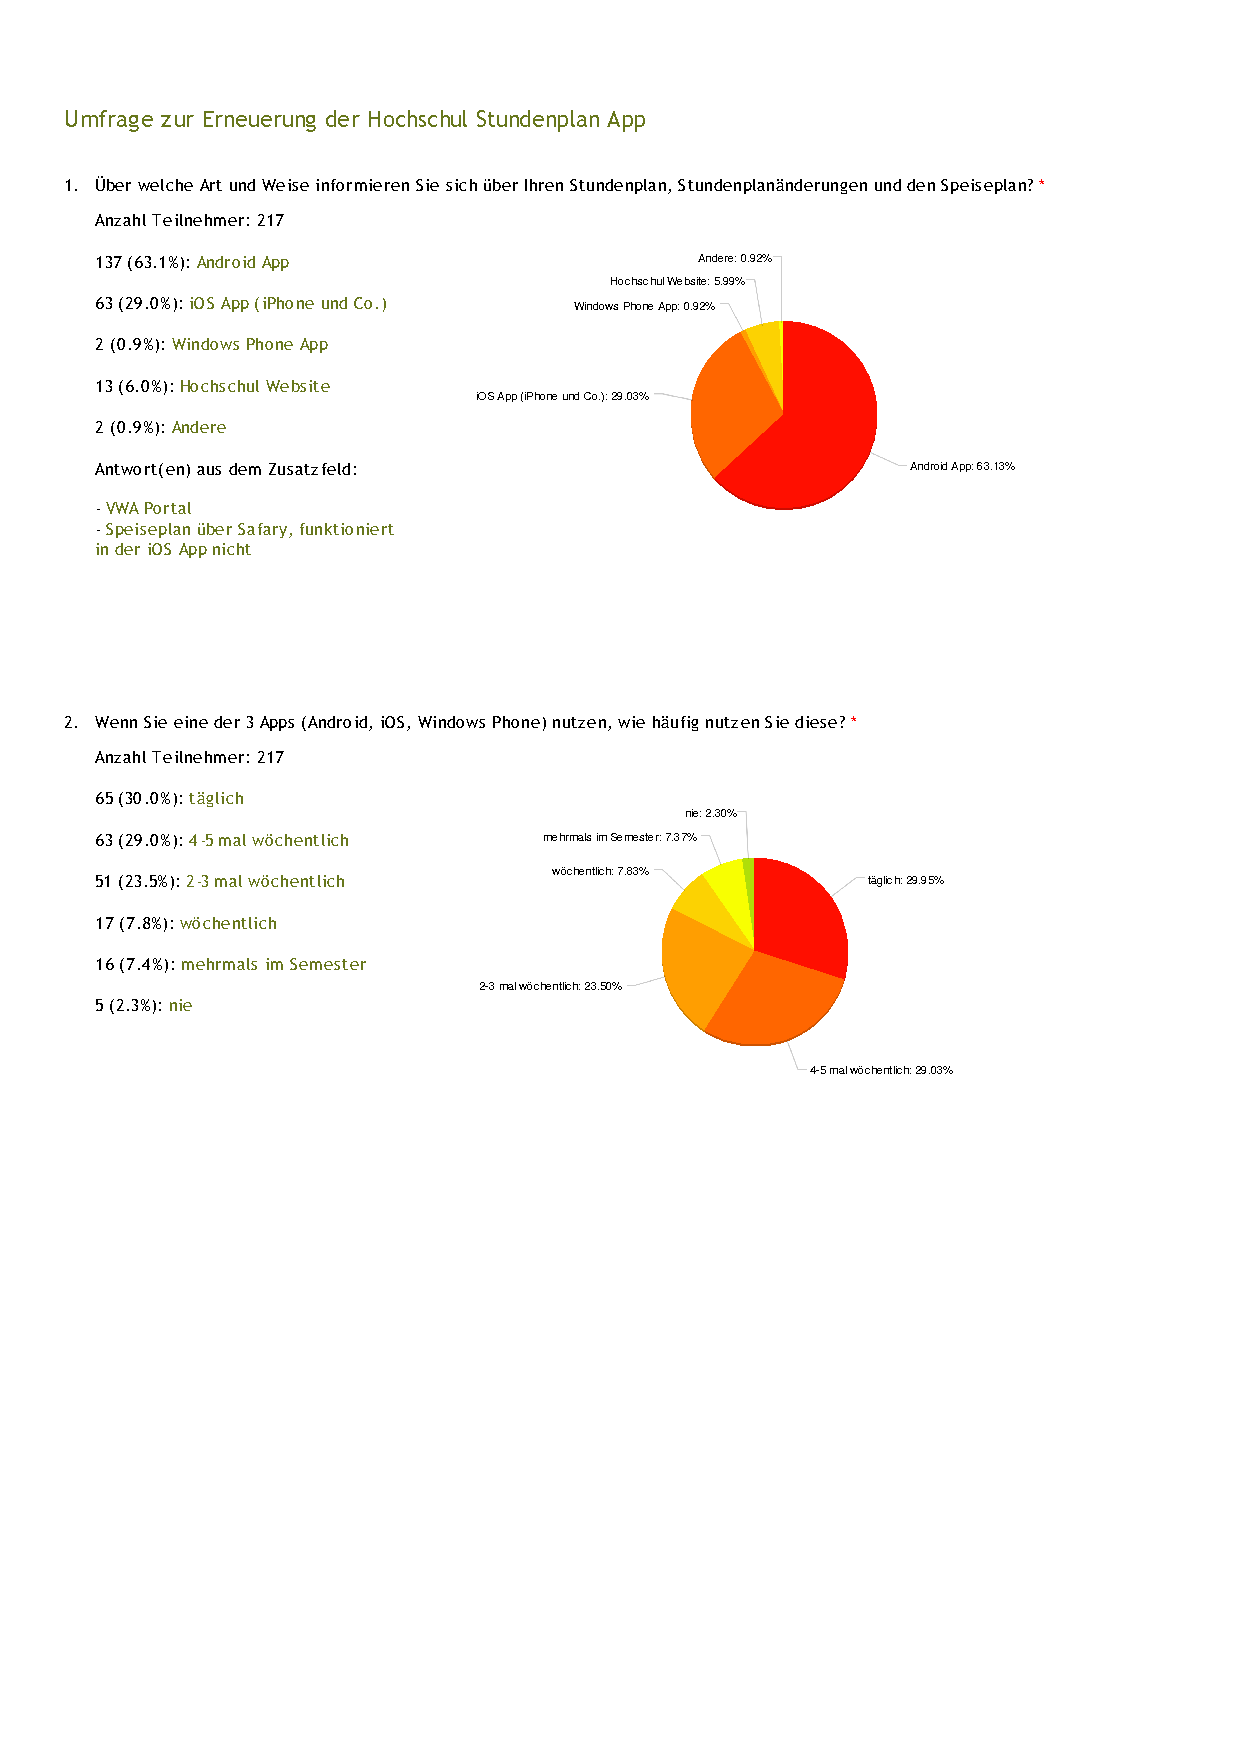
\includegraphics[
    width=\textwidth,
    height=\textheight,
    keepaspectratio
]{Kapiteln/Anhang/Inhalt/DE/umfrage_DE_Page1.pdf}
\vfill
\newpage
\noindent
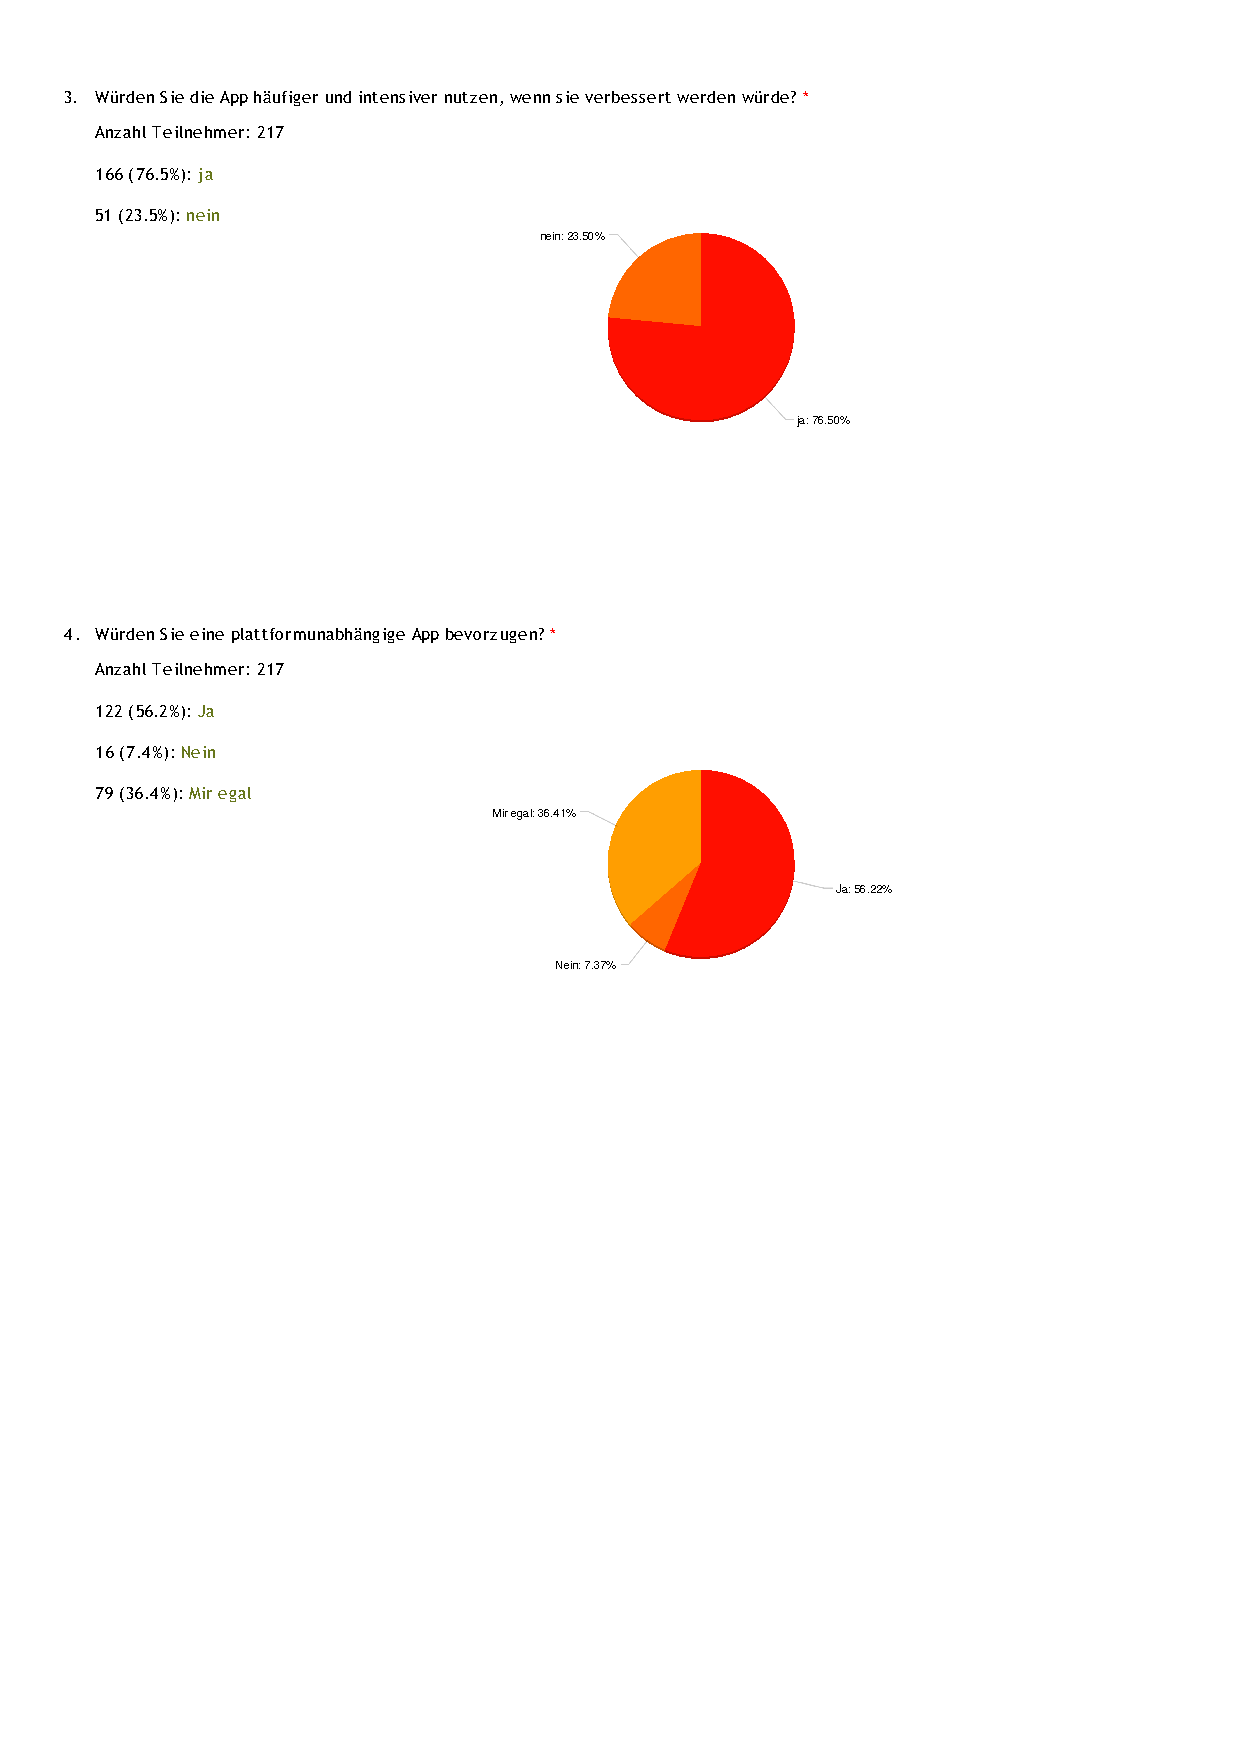
\includegraphics[
    width=\textwidth,
    height=\textheight,
    keepaspectratio
]{Kapiteln/Anhang/Inhalt/DE/umfrage_DE_Page2.pdf}
\vfill
\newpage
\noindent
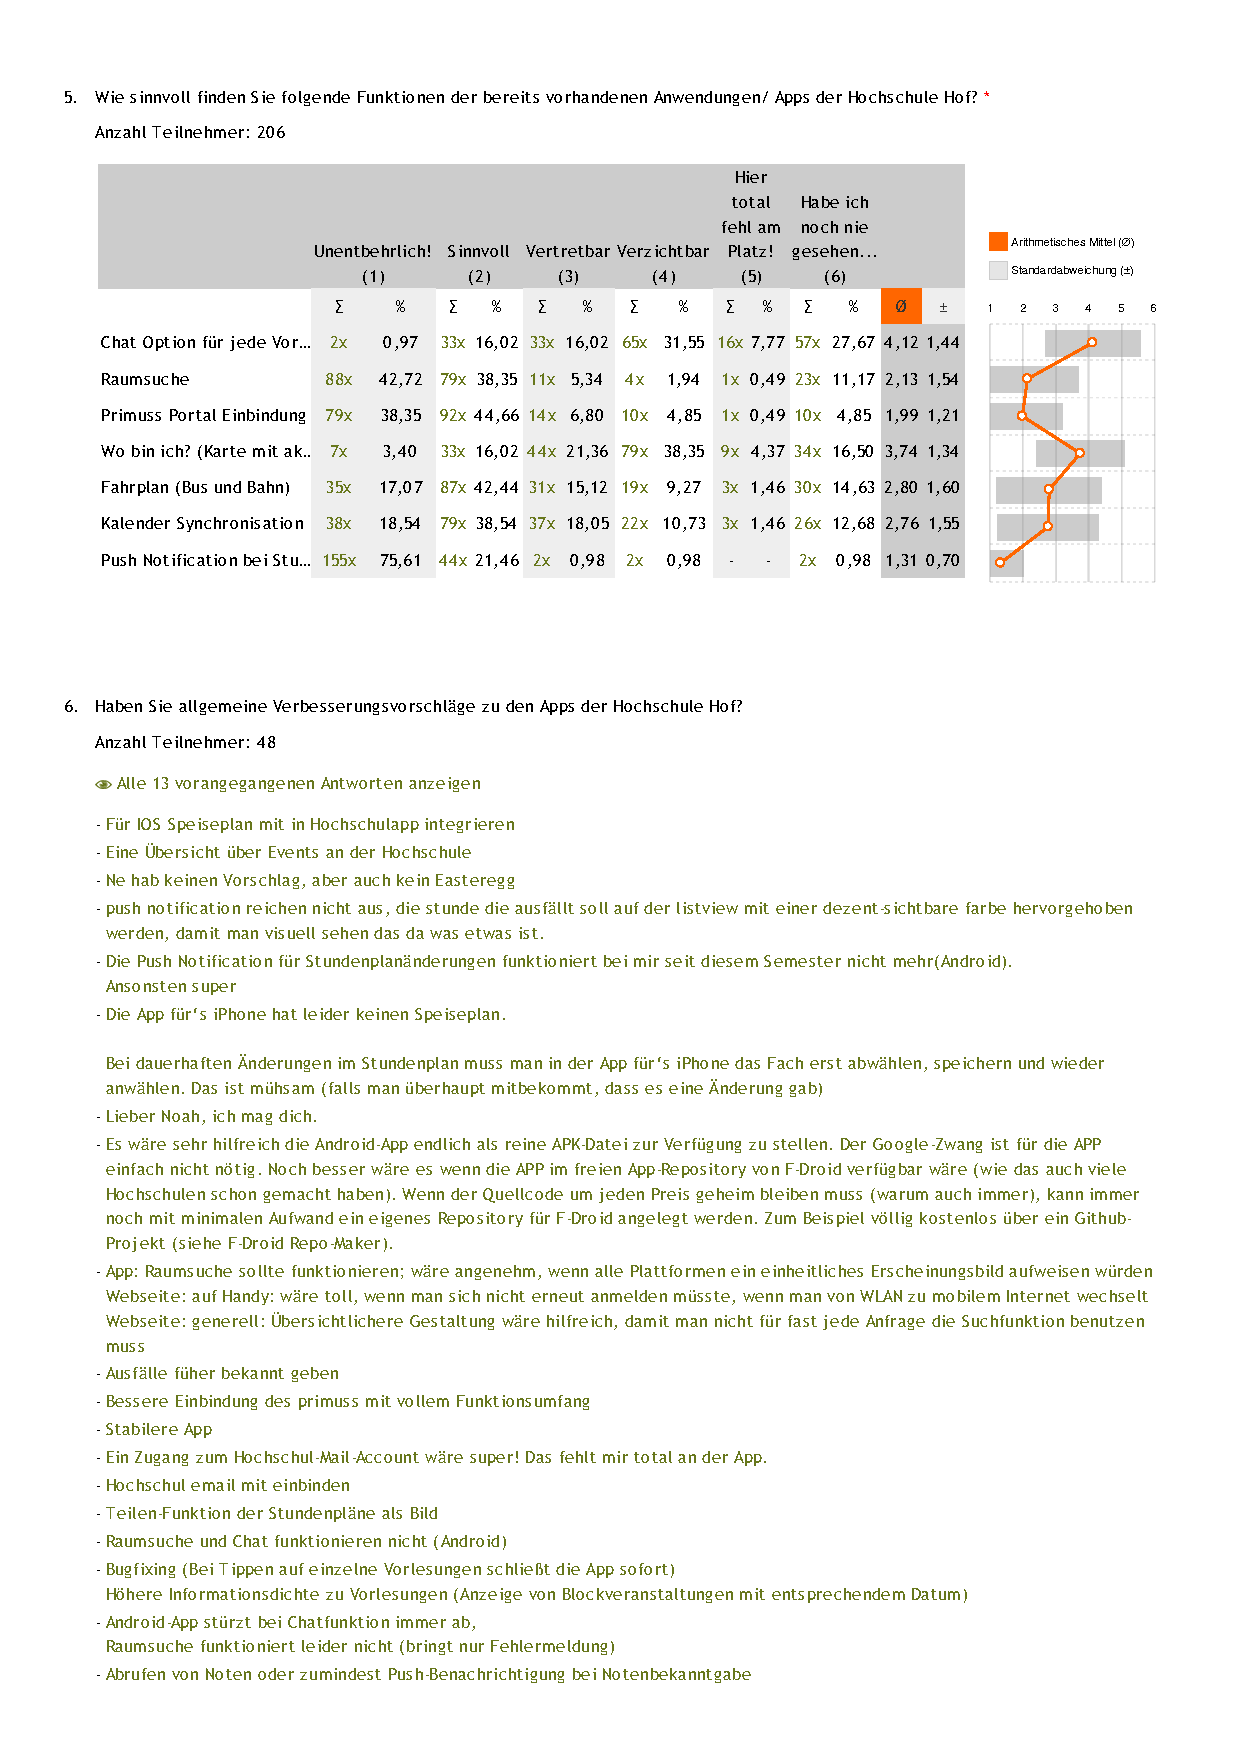
\includegraphics[
    width=\textwidth,
    height=\textheight,
    keepaspectratio
]{Kapiteln/Anhang/Inhalt/DE/umfrage_DE_Page3.pdf}
\vfill
\newpage
\noindent
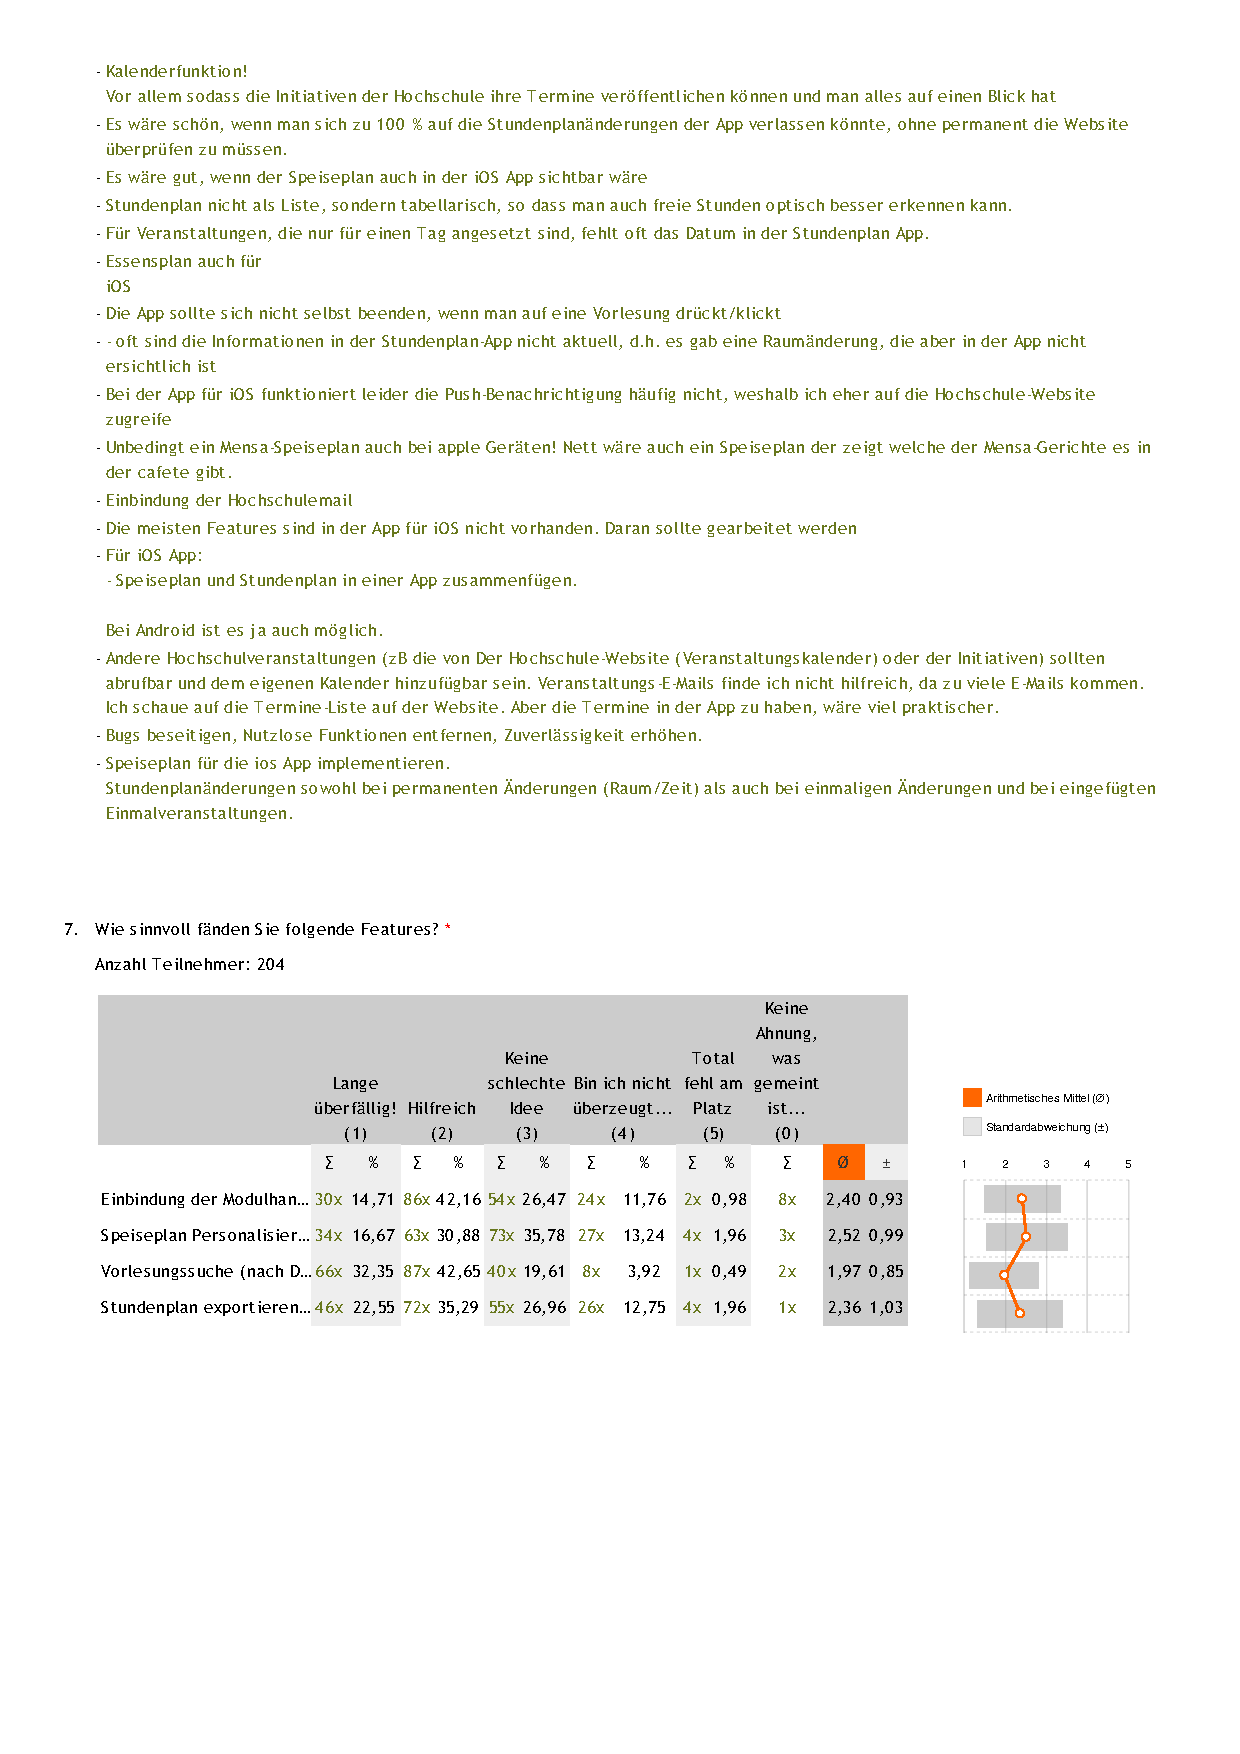
\includegraphics[
    width=\textwidth,
    height=\textheight,
    keepaspectratio
]{Kapiteln/Anhang/Inhalt/DE/umfrage_DE_Page4.pdf}
\vfill
\newpage
\noindent
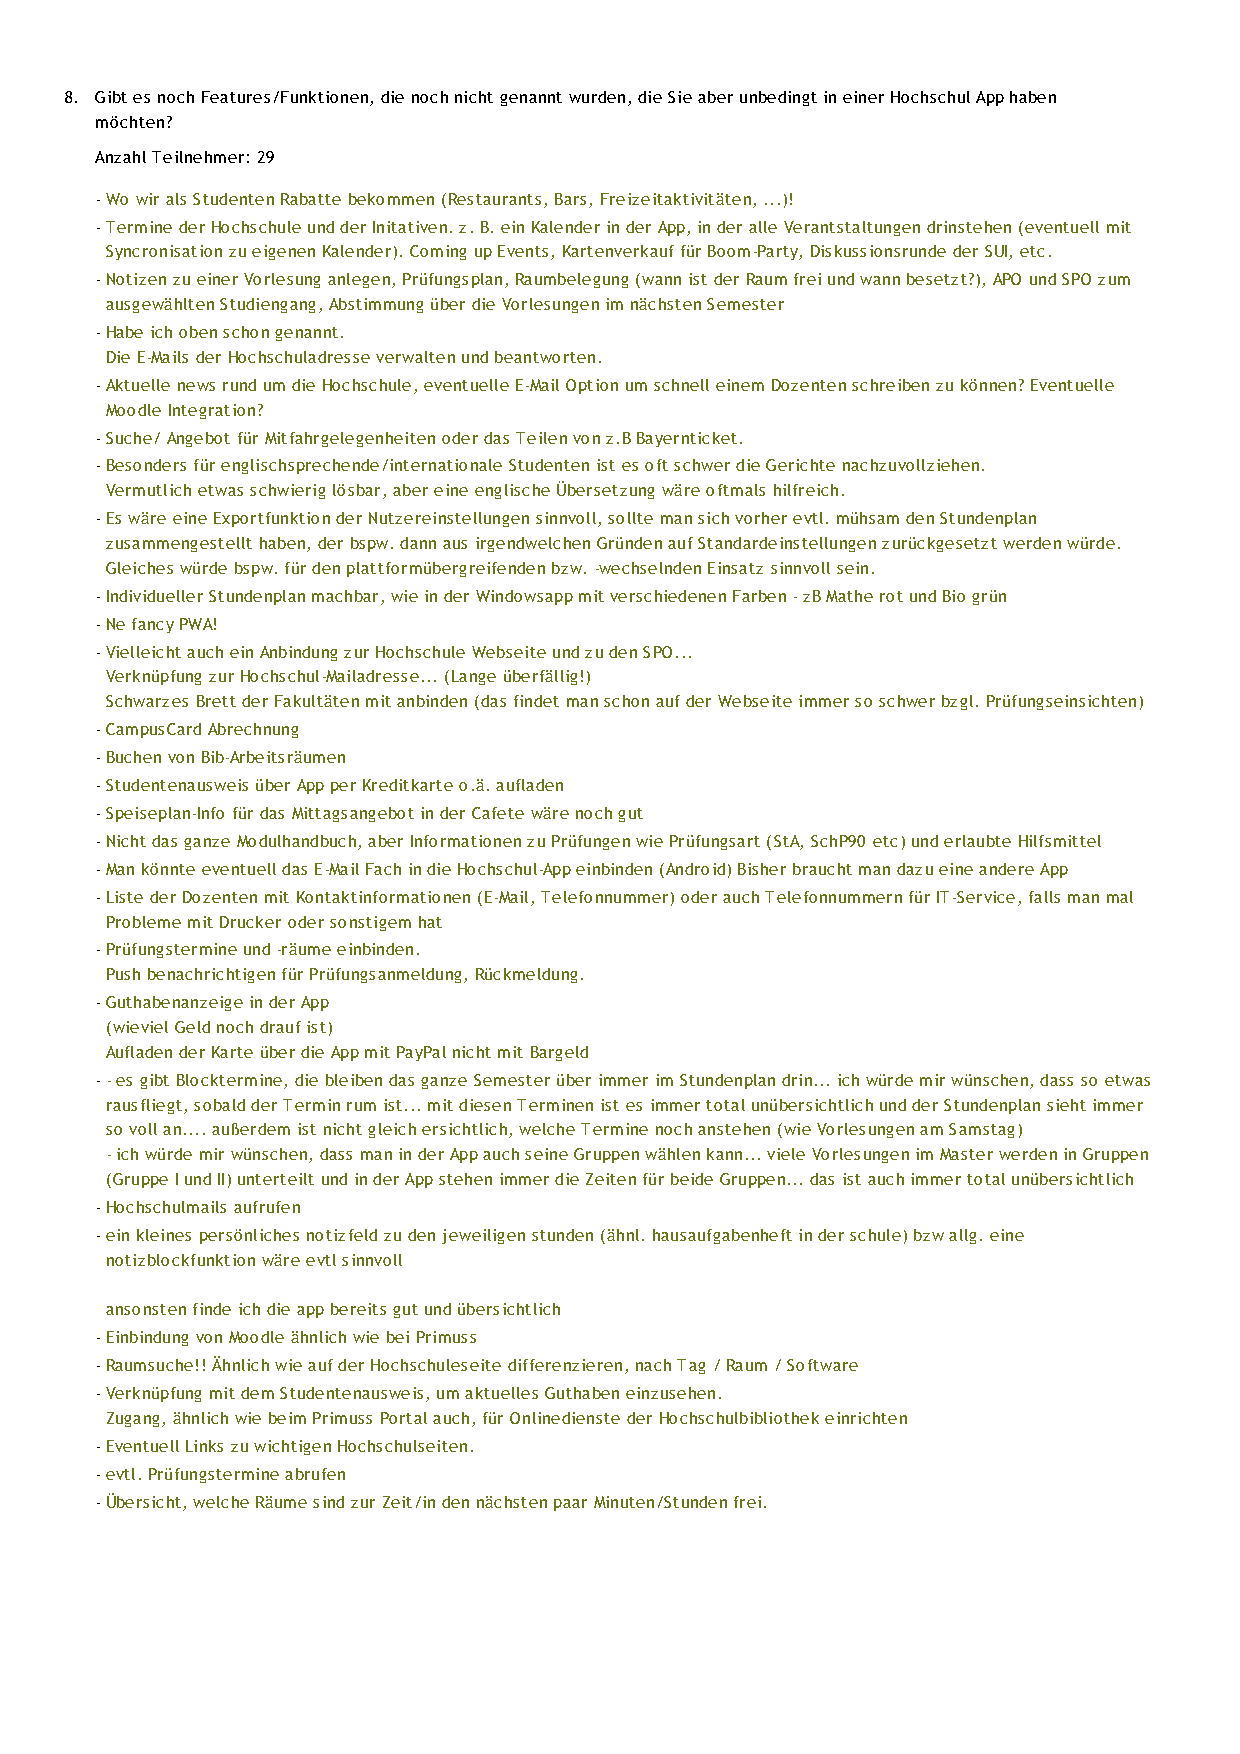
\includegraphics[
    width=\textwidth,
    height=\textheight,
    keepaspectratio
]{Kapiteln/Anhang/Inhalt/DE/umfrage_DE_Page5.pdf}
\vfill
\newpage
\noindent
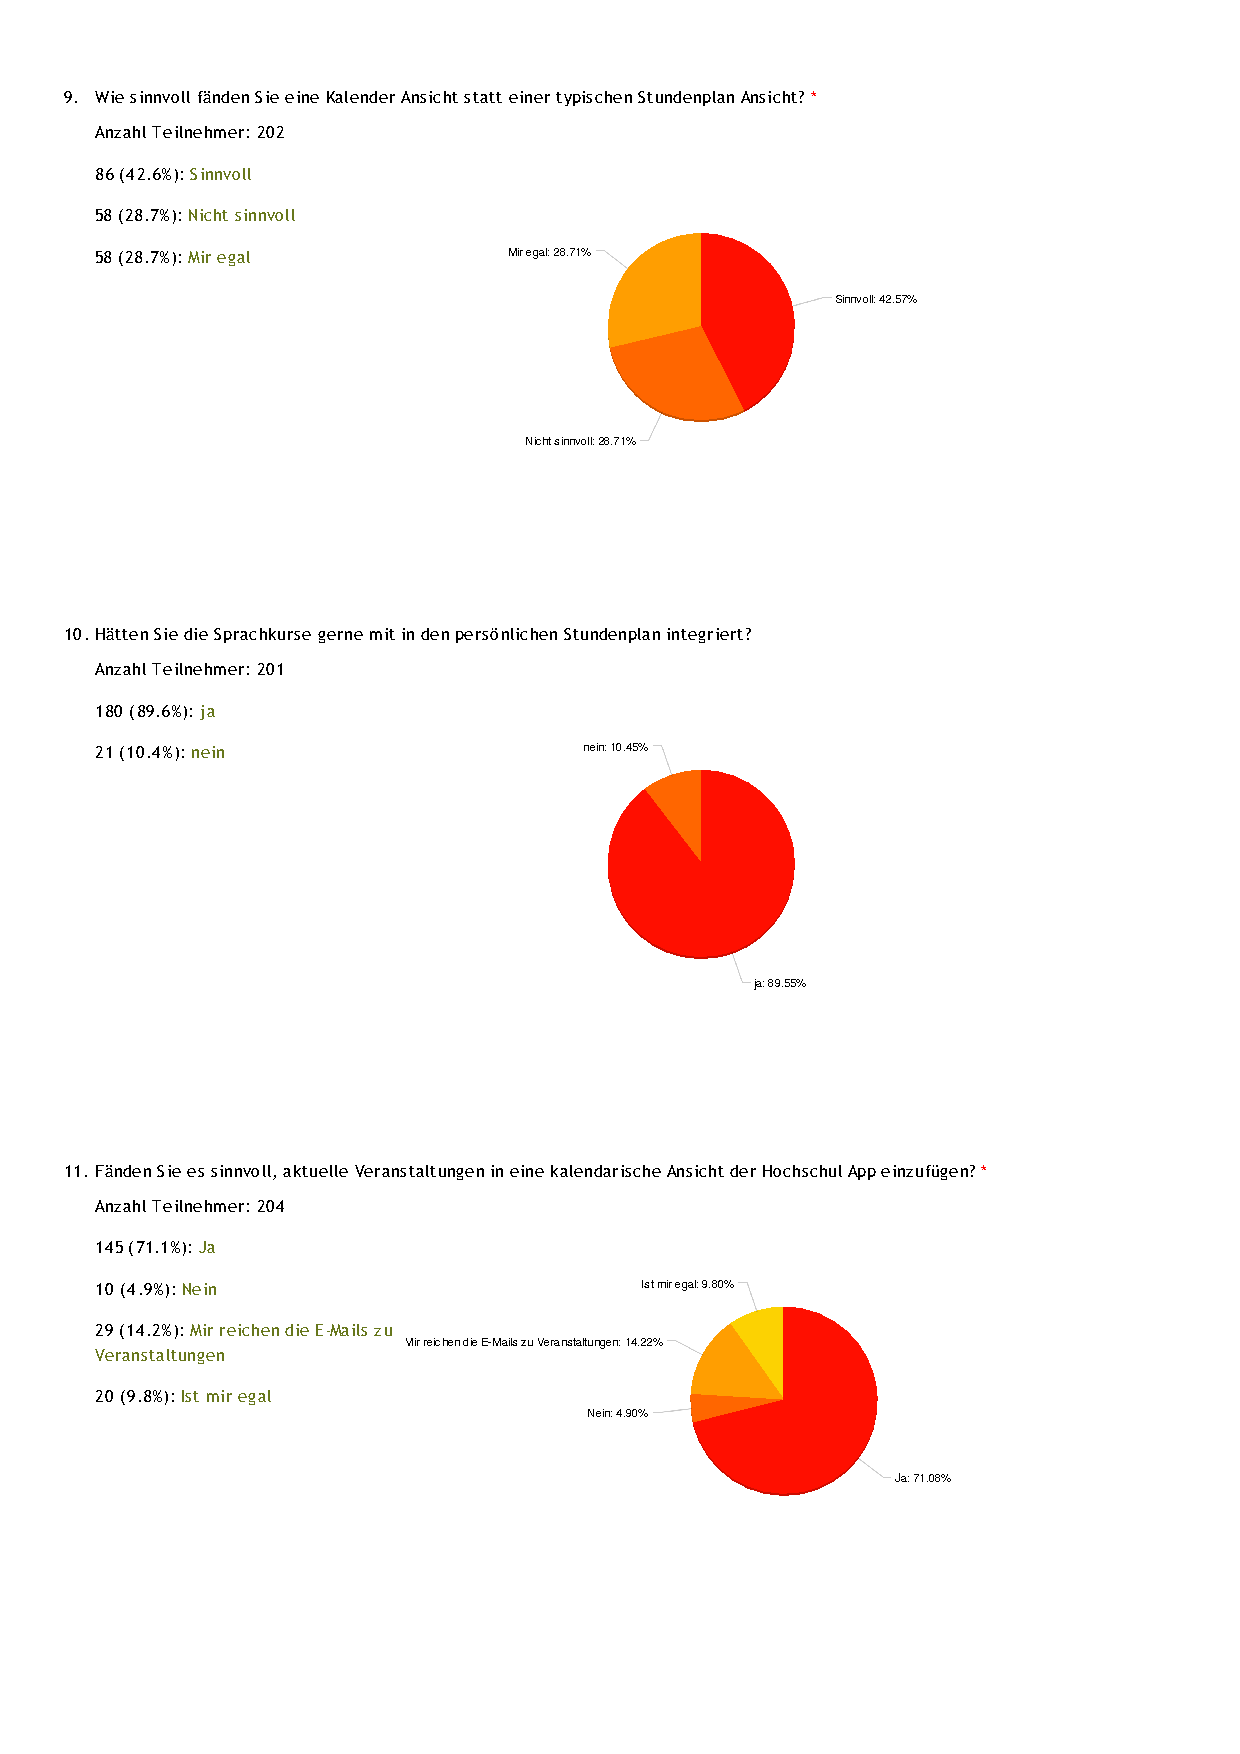
\includegraphics[
    width=\textwidth,
    height=\textheight,
    keepaspectratio
]{Kapiteln/Anhang/Inhalt/DE/umfrage_DE_Page6.pdf}
\vfill
\newpage
\noindent
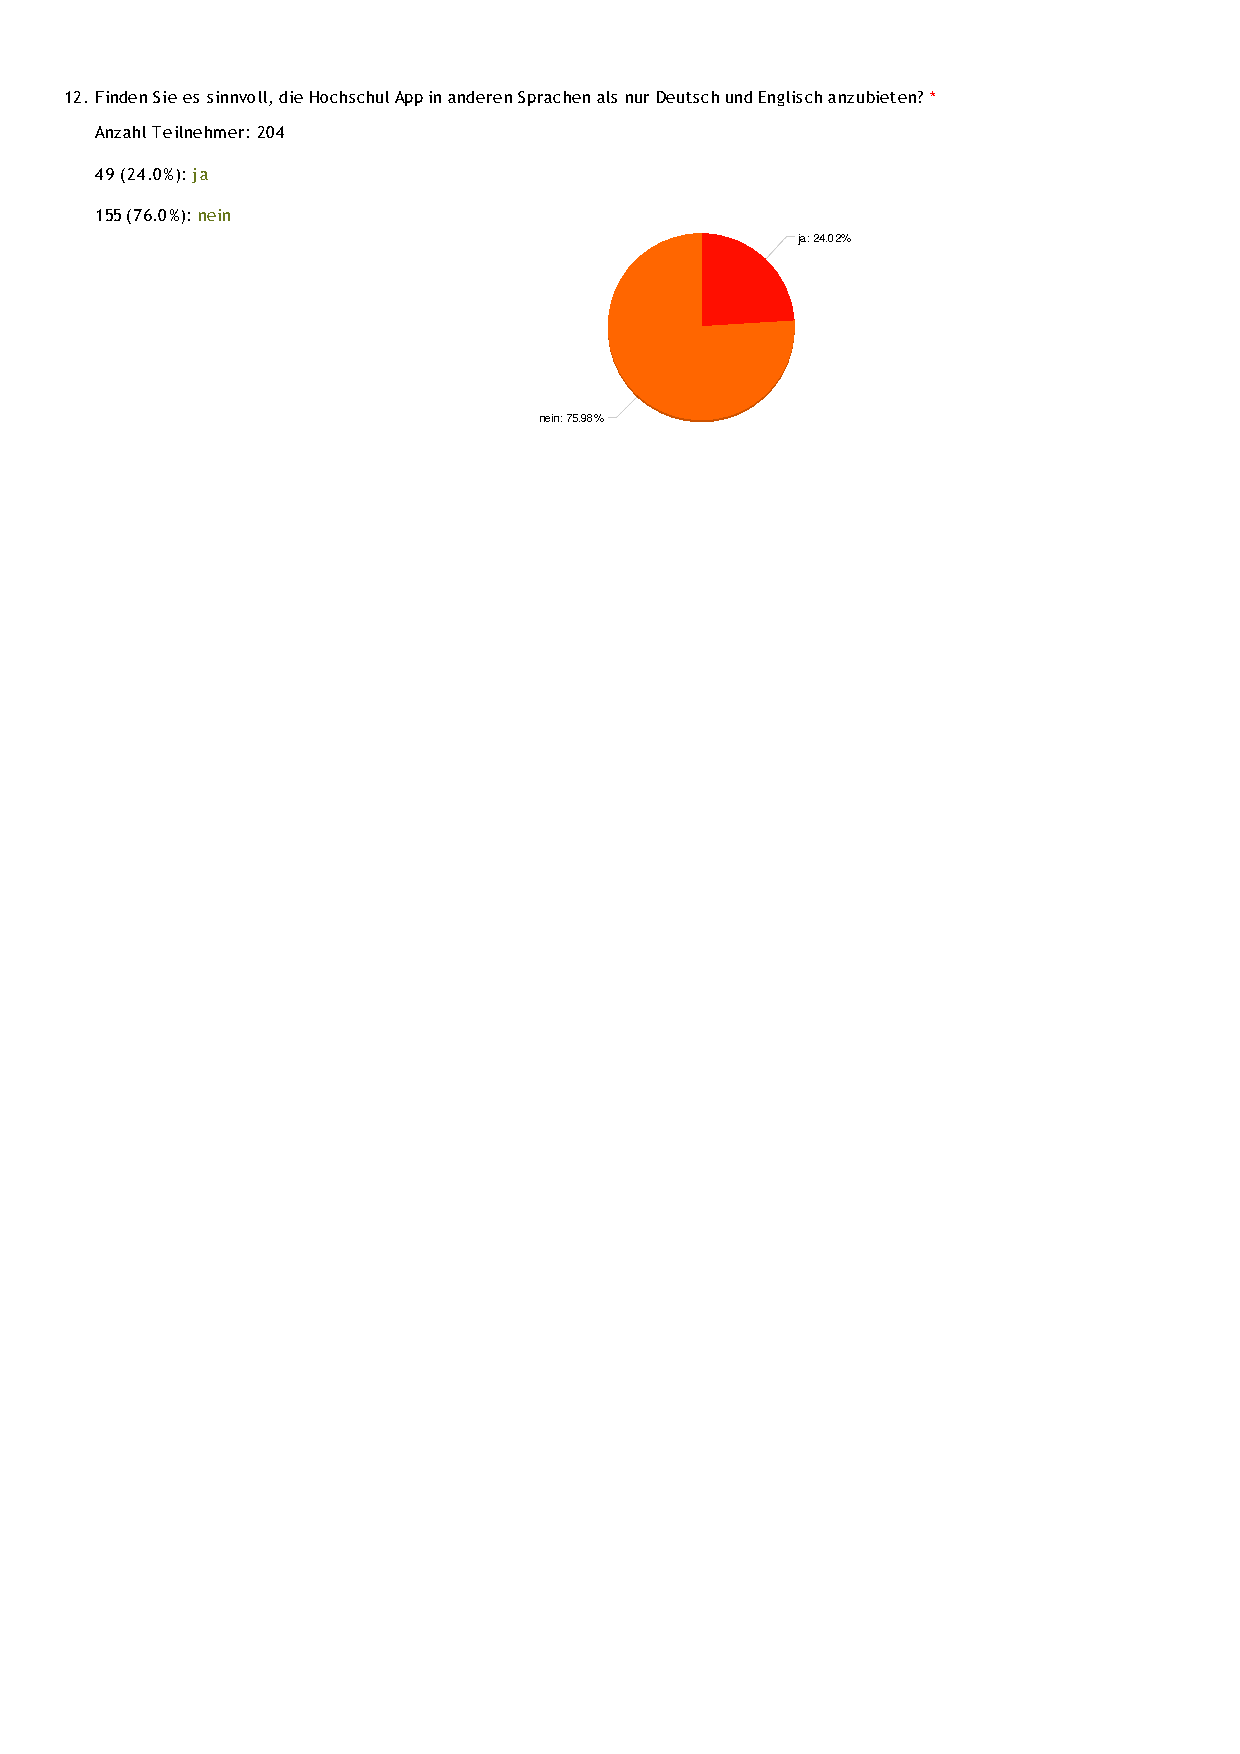
\includegraphics[
    width=\textwidth,
    height=\textheight,
    keepaspectratio
]{Kapiteln/Anhang/Inhalt/DE/umfrage_DE_Page7.pdf}
\vfill
\newpage
\noindent
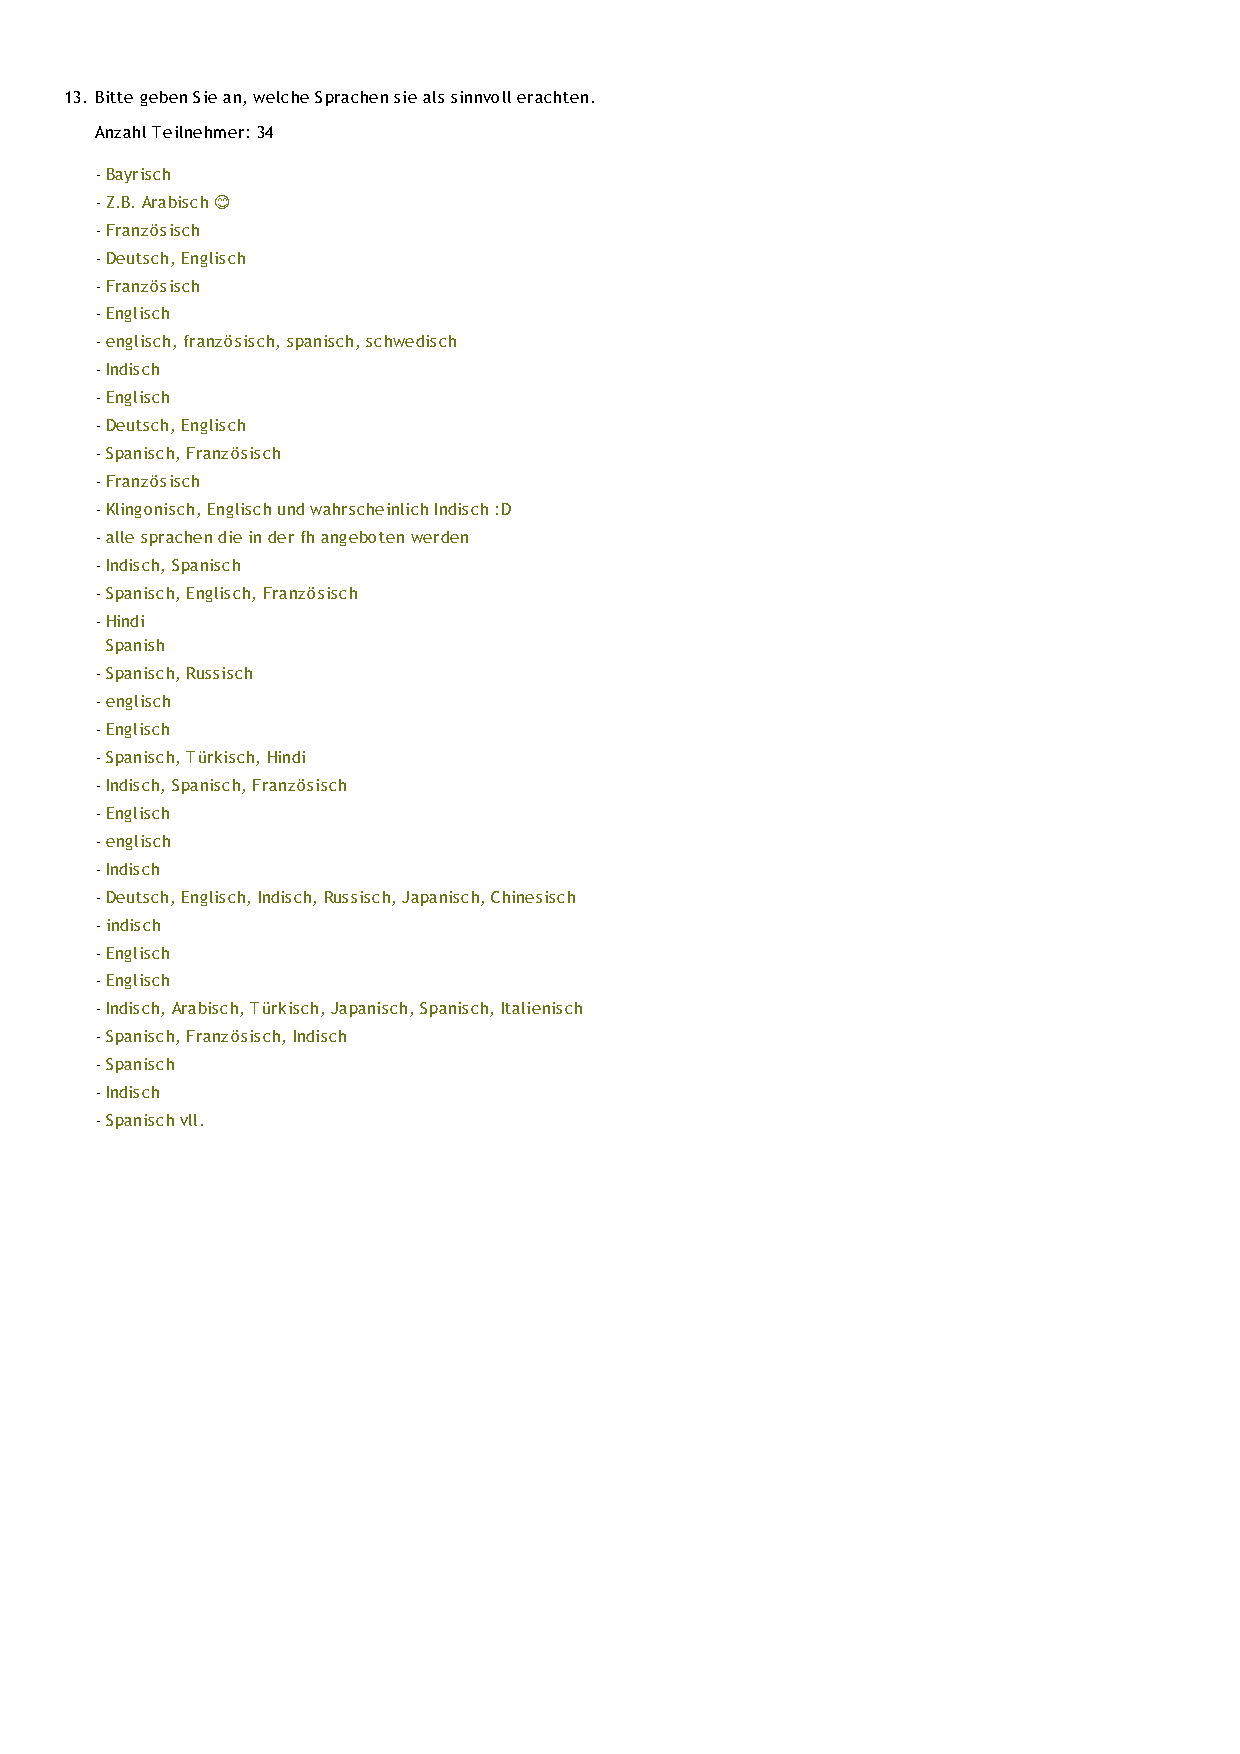
\includegraphics[
    width=\textwidth,
    height=\textheight,
    keepaspectratio
]{Kapiteln/Anhang/Inhalt/DE/umfrage_DE_Page8.pdf}
\vfill
\newpage
\noindent
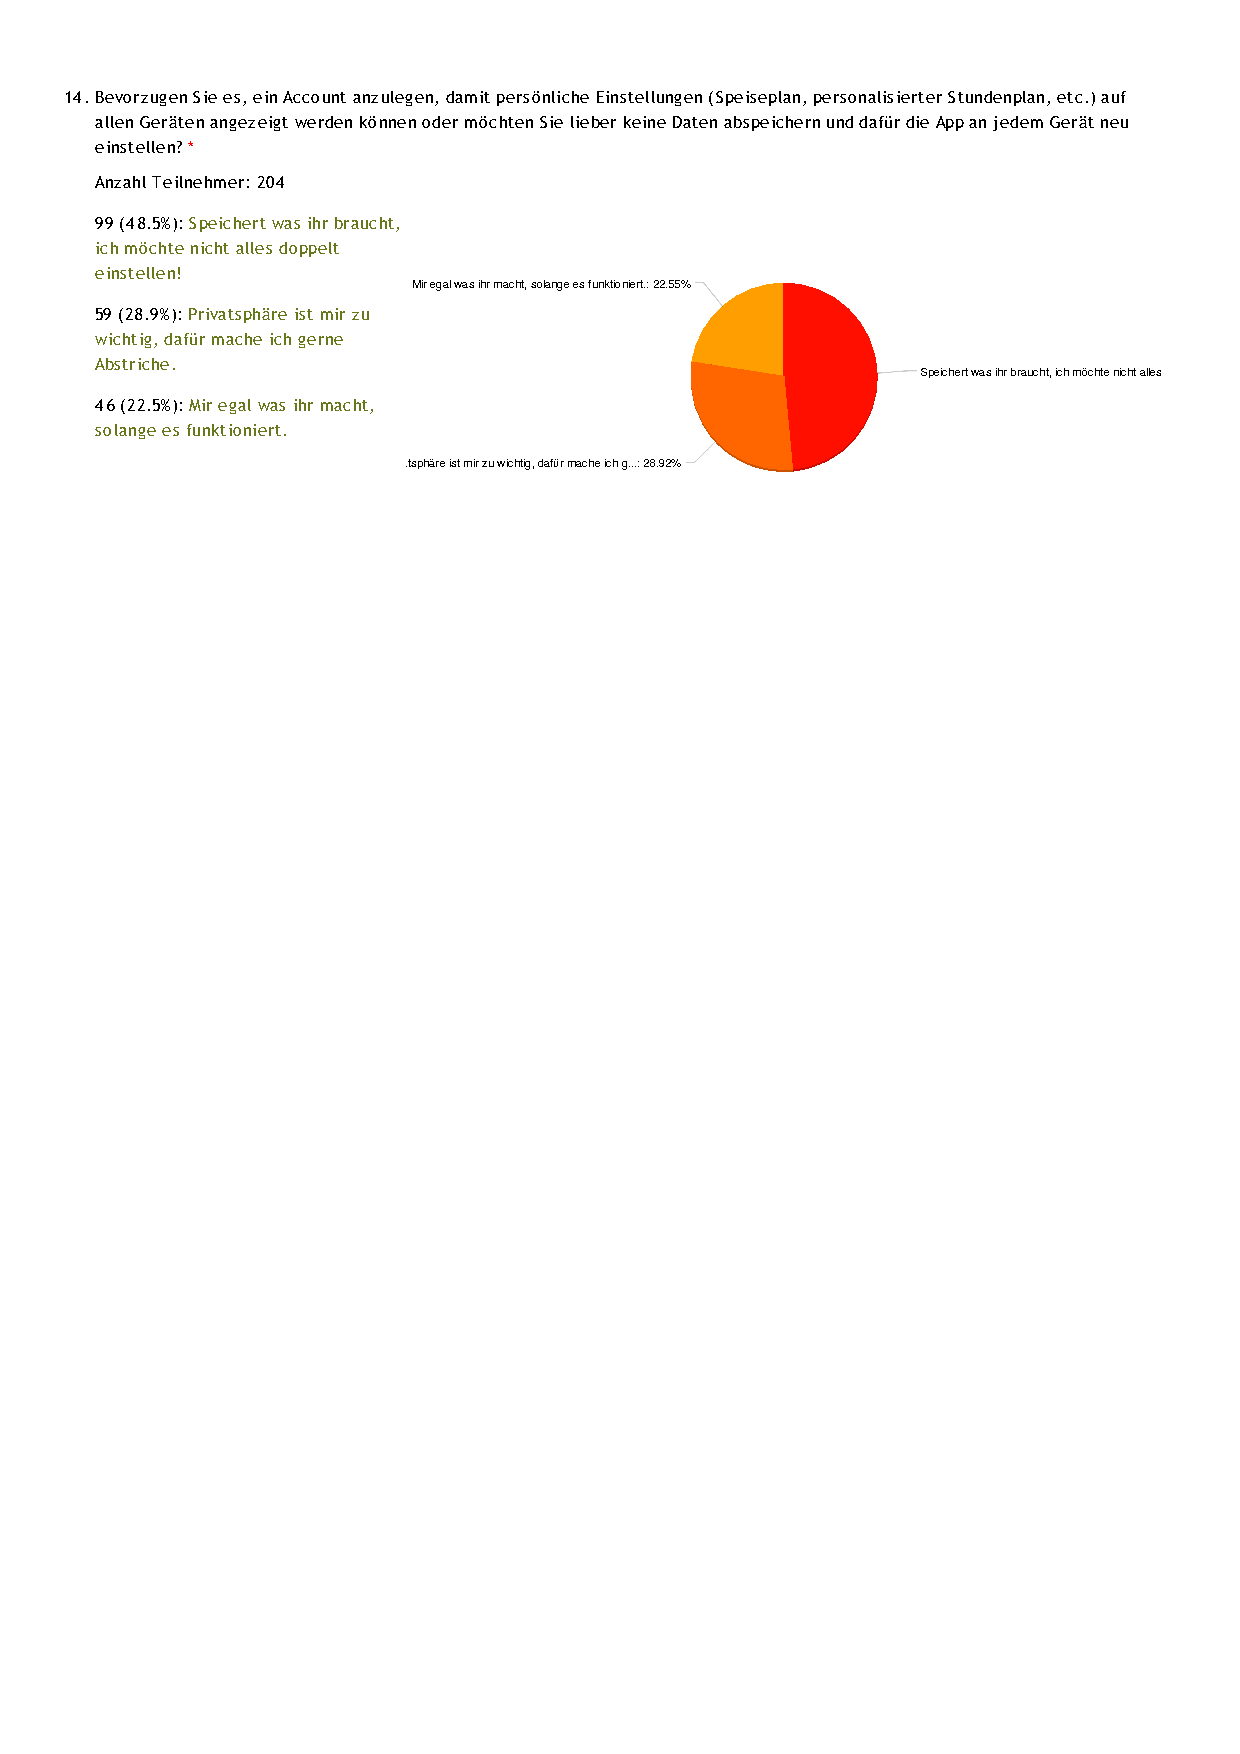
\includegraphics[
    width=\textwidth,
    height=\textheight,
    keepaspectratio
]{Kapiteln/Anhang/Inhalt/DE/umfrage_DE_Page9.pdf}
\vfill
\newpage
\noindent
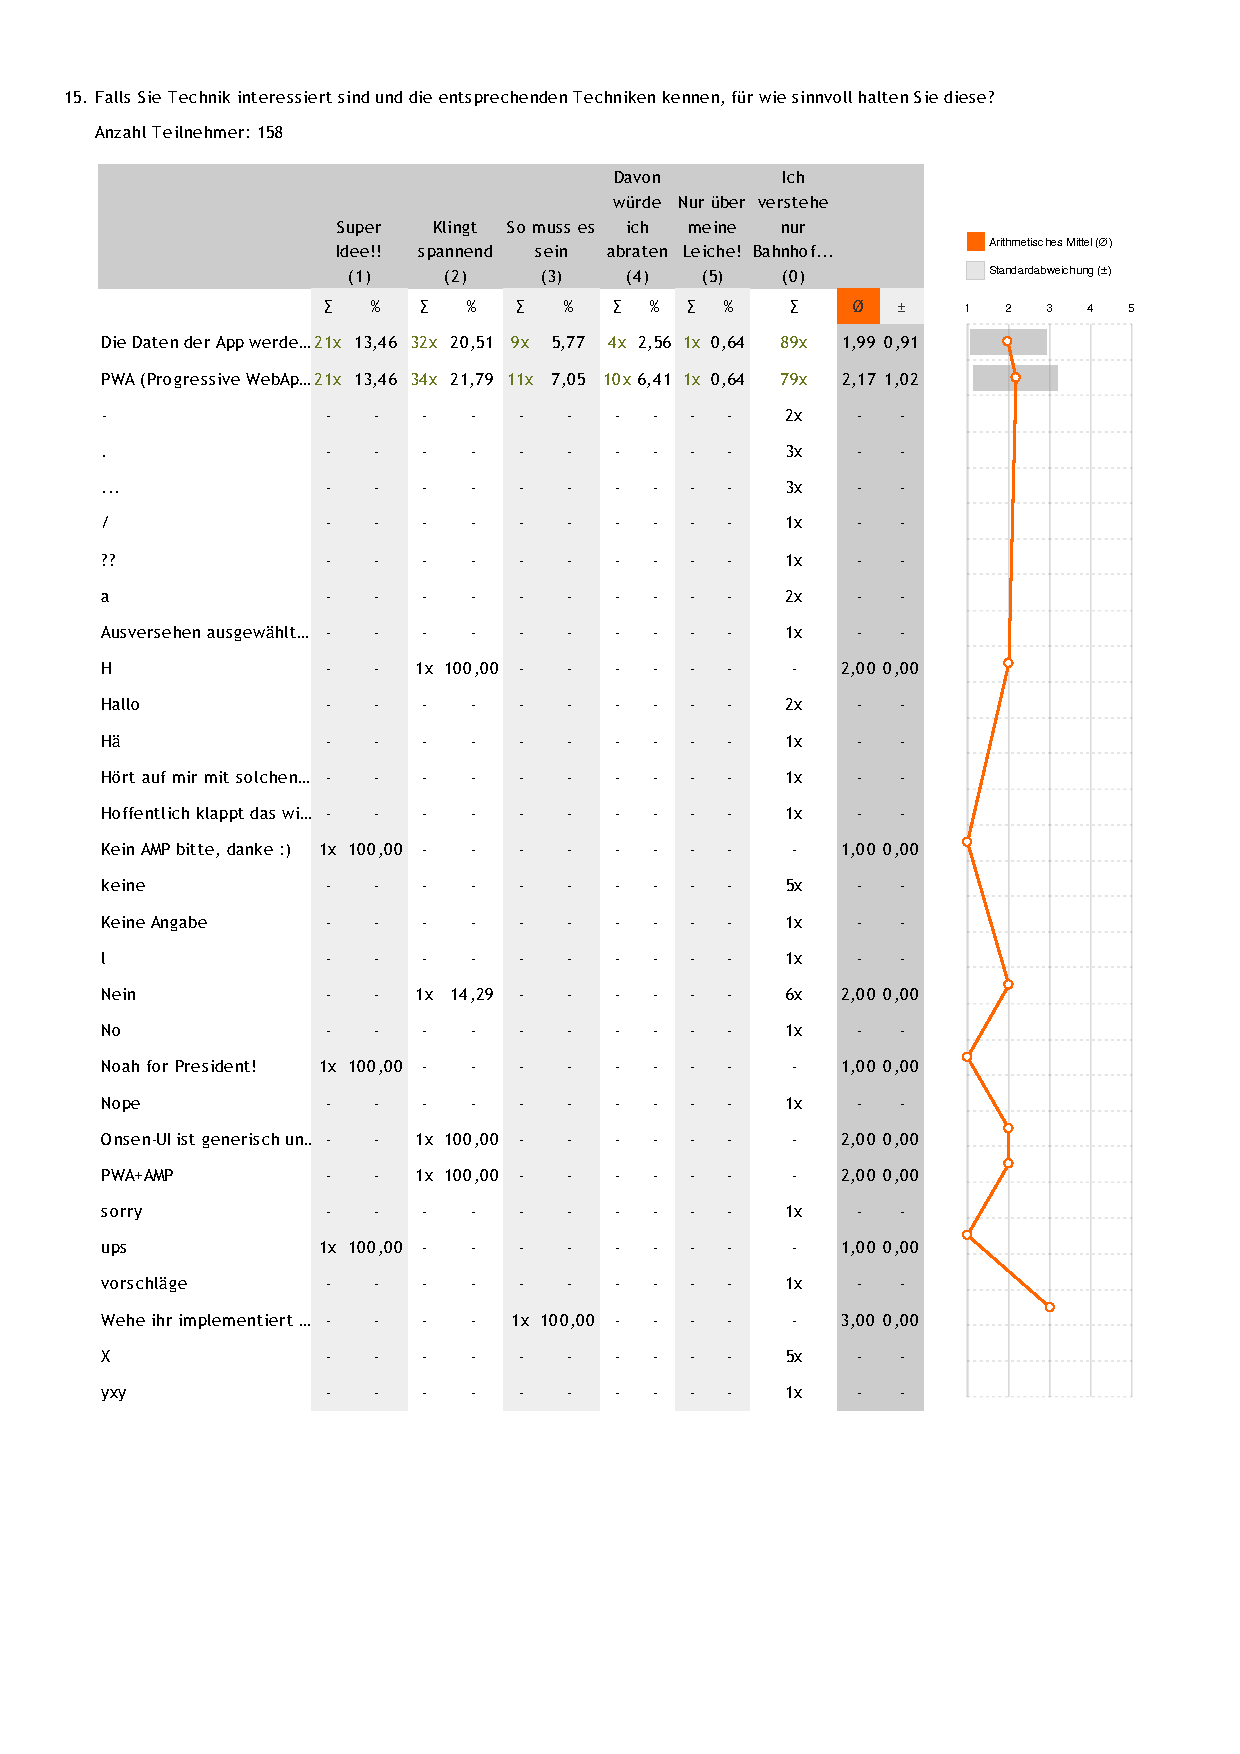
\includegraphics[
    width=\textwidth,
    height=\textheight,
    keepaspectratio
]{Kapiteln/Anhang/Inhalt/DE/umfrage_DE_Page10.pdf}
\vfill
\newpage

\section*{Internationale Umfrage}
\addcontentsline{toc}{subsection}{Internationale Umfrage}

\noindent
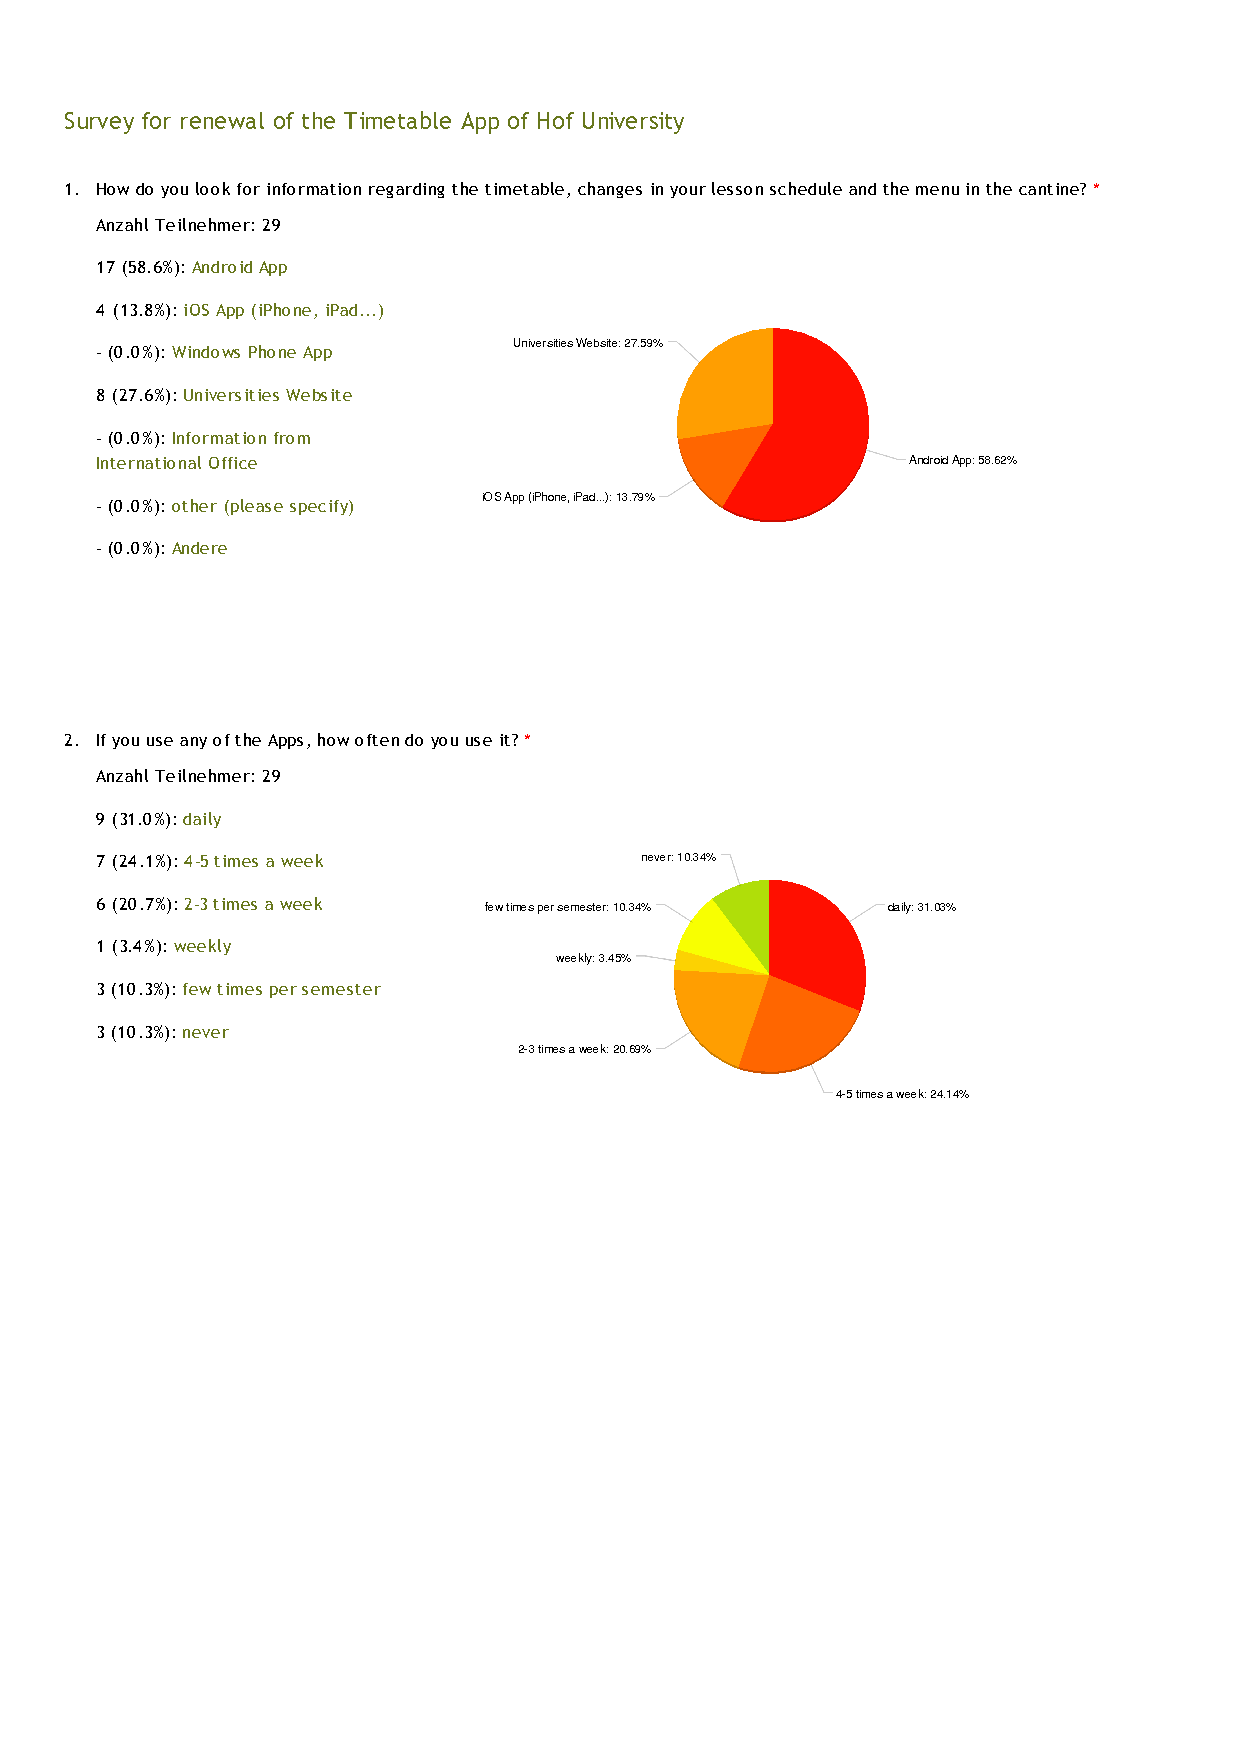
\includegraphics[
    width=\textwidth,
    height=\textheight,
    keepaspectratio
]{Kapiteln/Anhang/Inhalt/EN/survey_EN_Page1.pdf}
\vfill
\newpage
\noindent
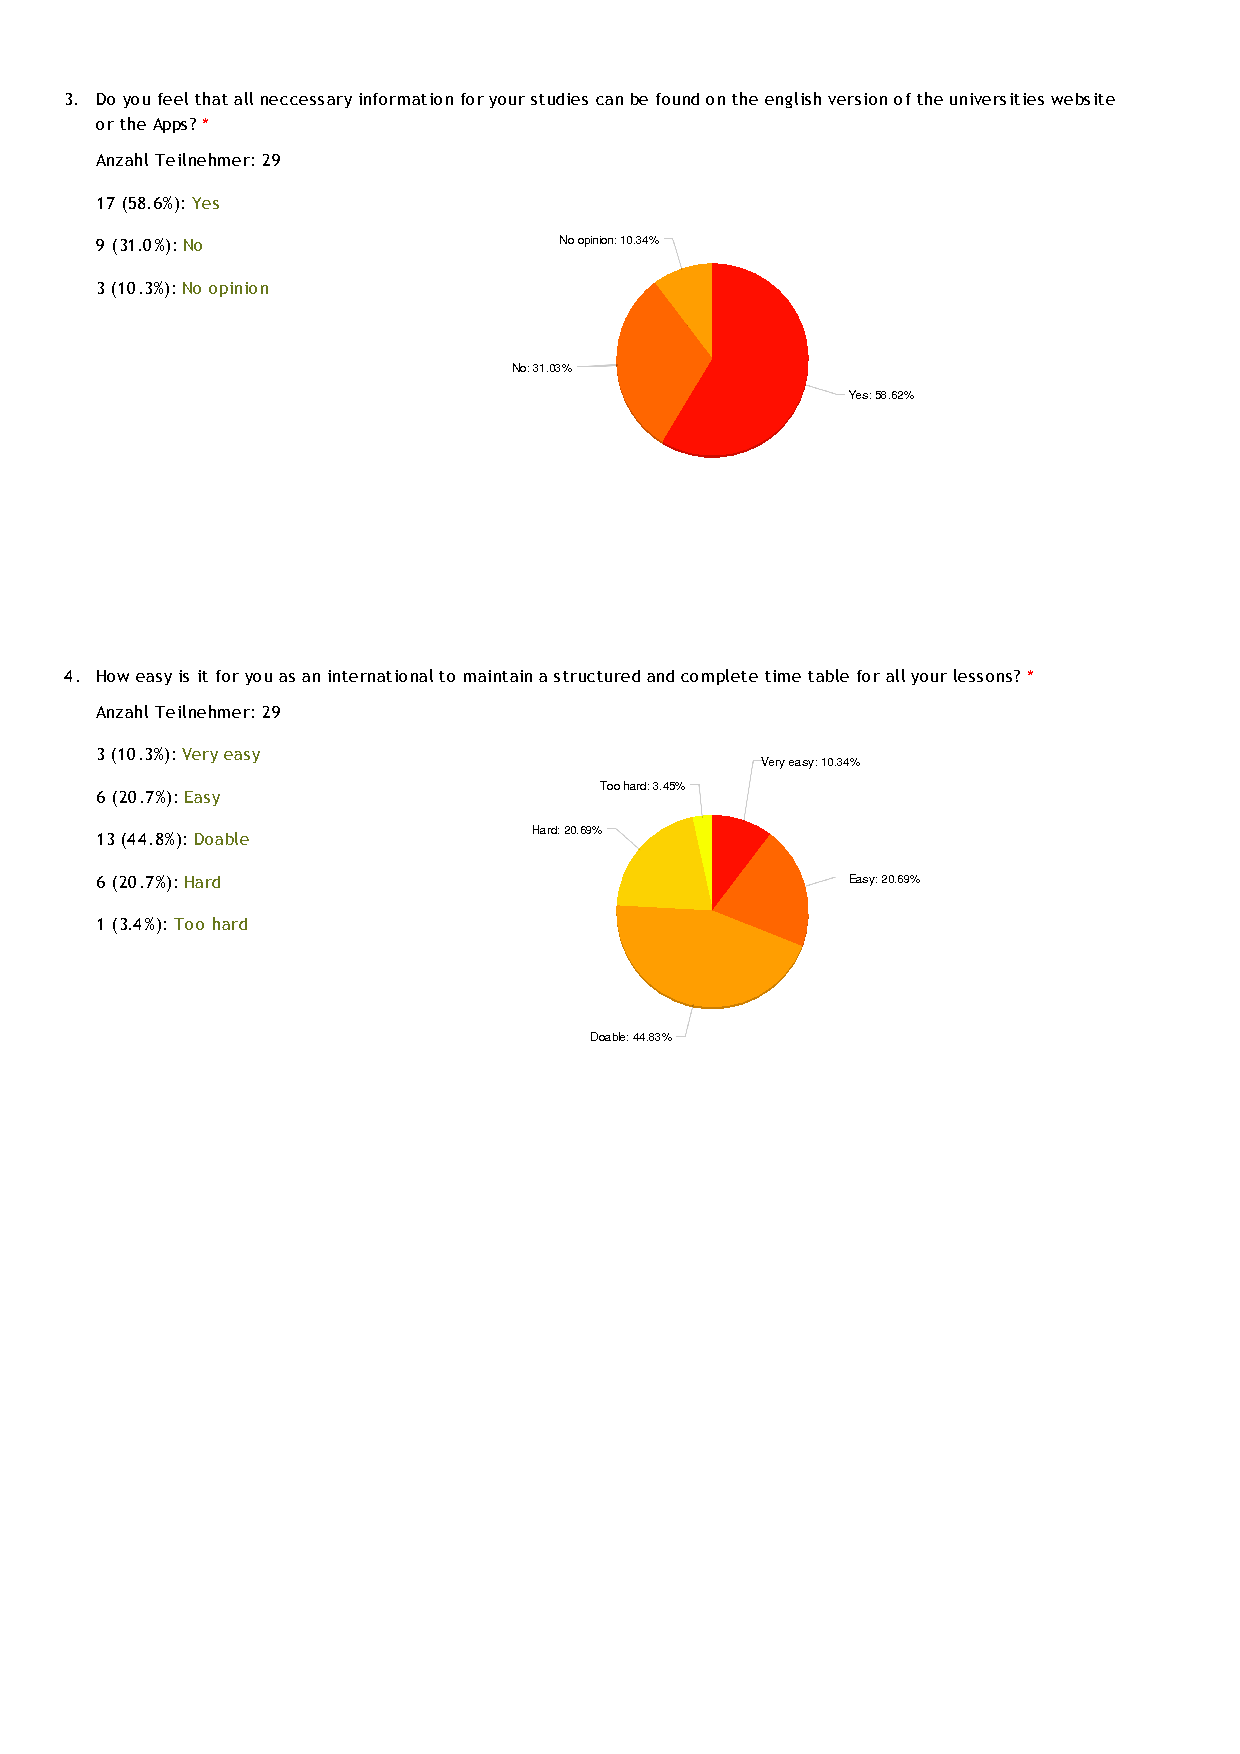
\includegraphics[
    width=\textwidth,
    height=\textheight,
    keepaspectratio
]{Kapiteln/Anhang/Inhalt/EN/survey_EN_Page2.pdf}
\vfill
\newpage
\noindent
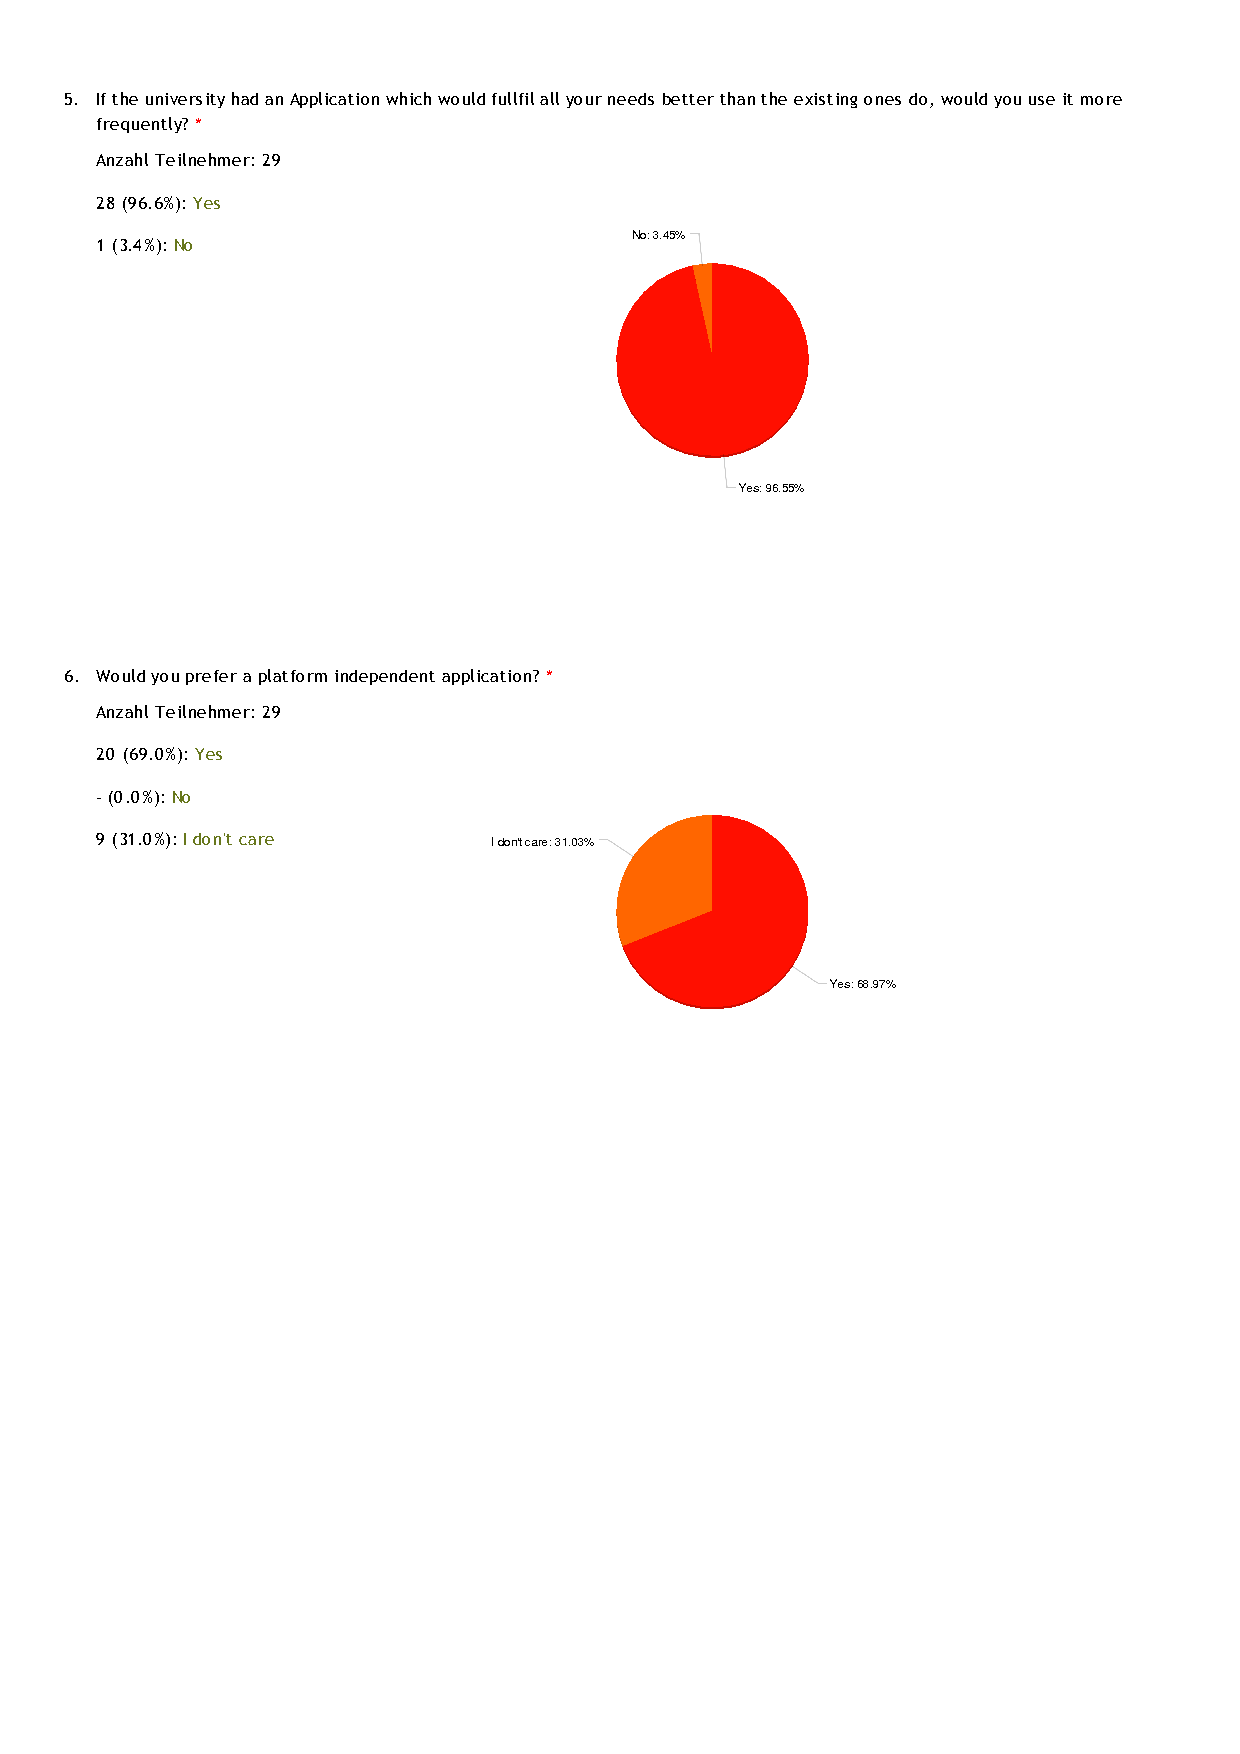
\includegraphics[
    width=\textwidth,
    height=\textheight,
    keepaspectratio
]{Kapiteln/Anhang/Inhalt/EN/survey_EN_Page3.pdf}
\vfill
\newpage
\noindent
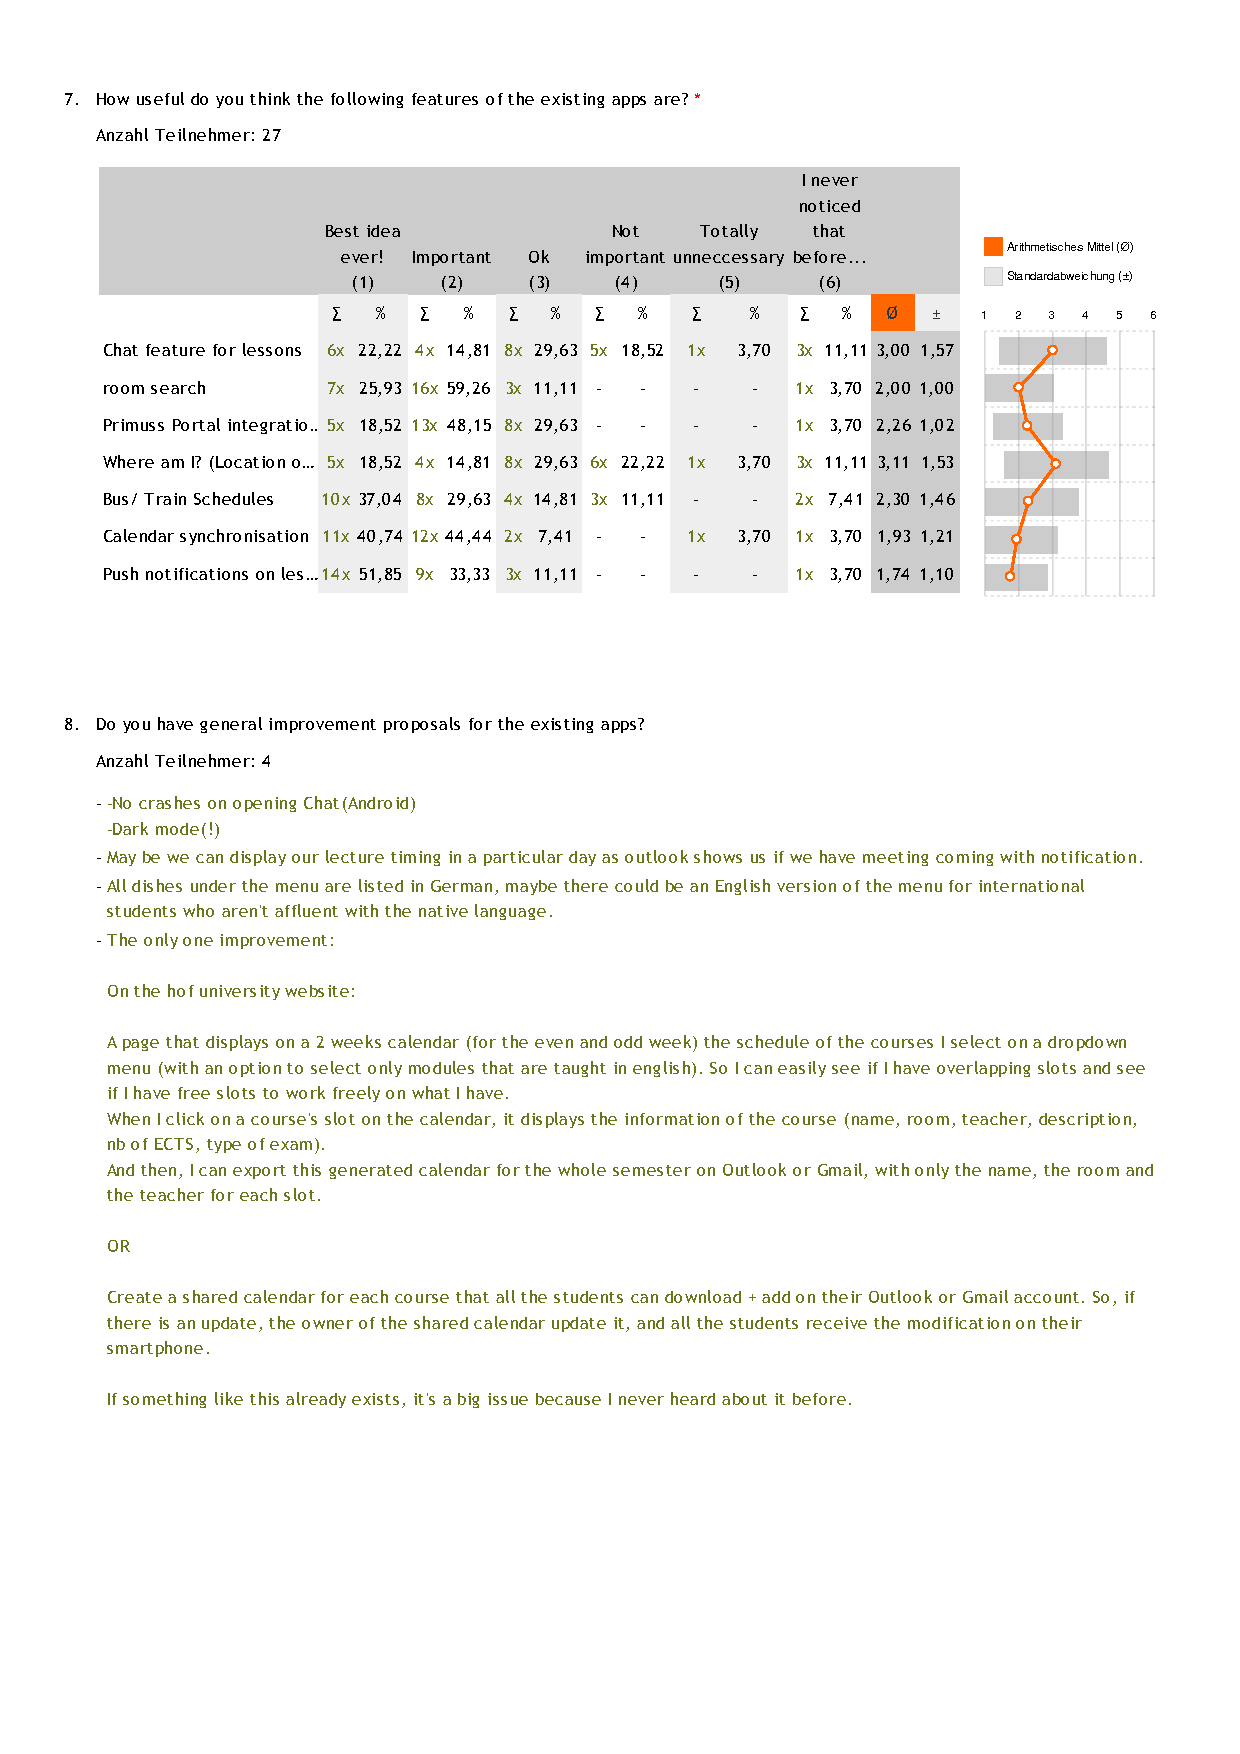
\includegraphics[
    width=\textwidth,
    height=\textheight,
    keepaspectratio
]{Kapiteln/Anhang/Inhalt/EN/survey_EN_Page4.pdf}
\vfill
\newpage
\noindent
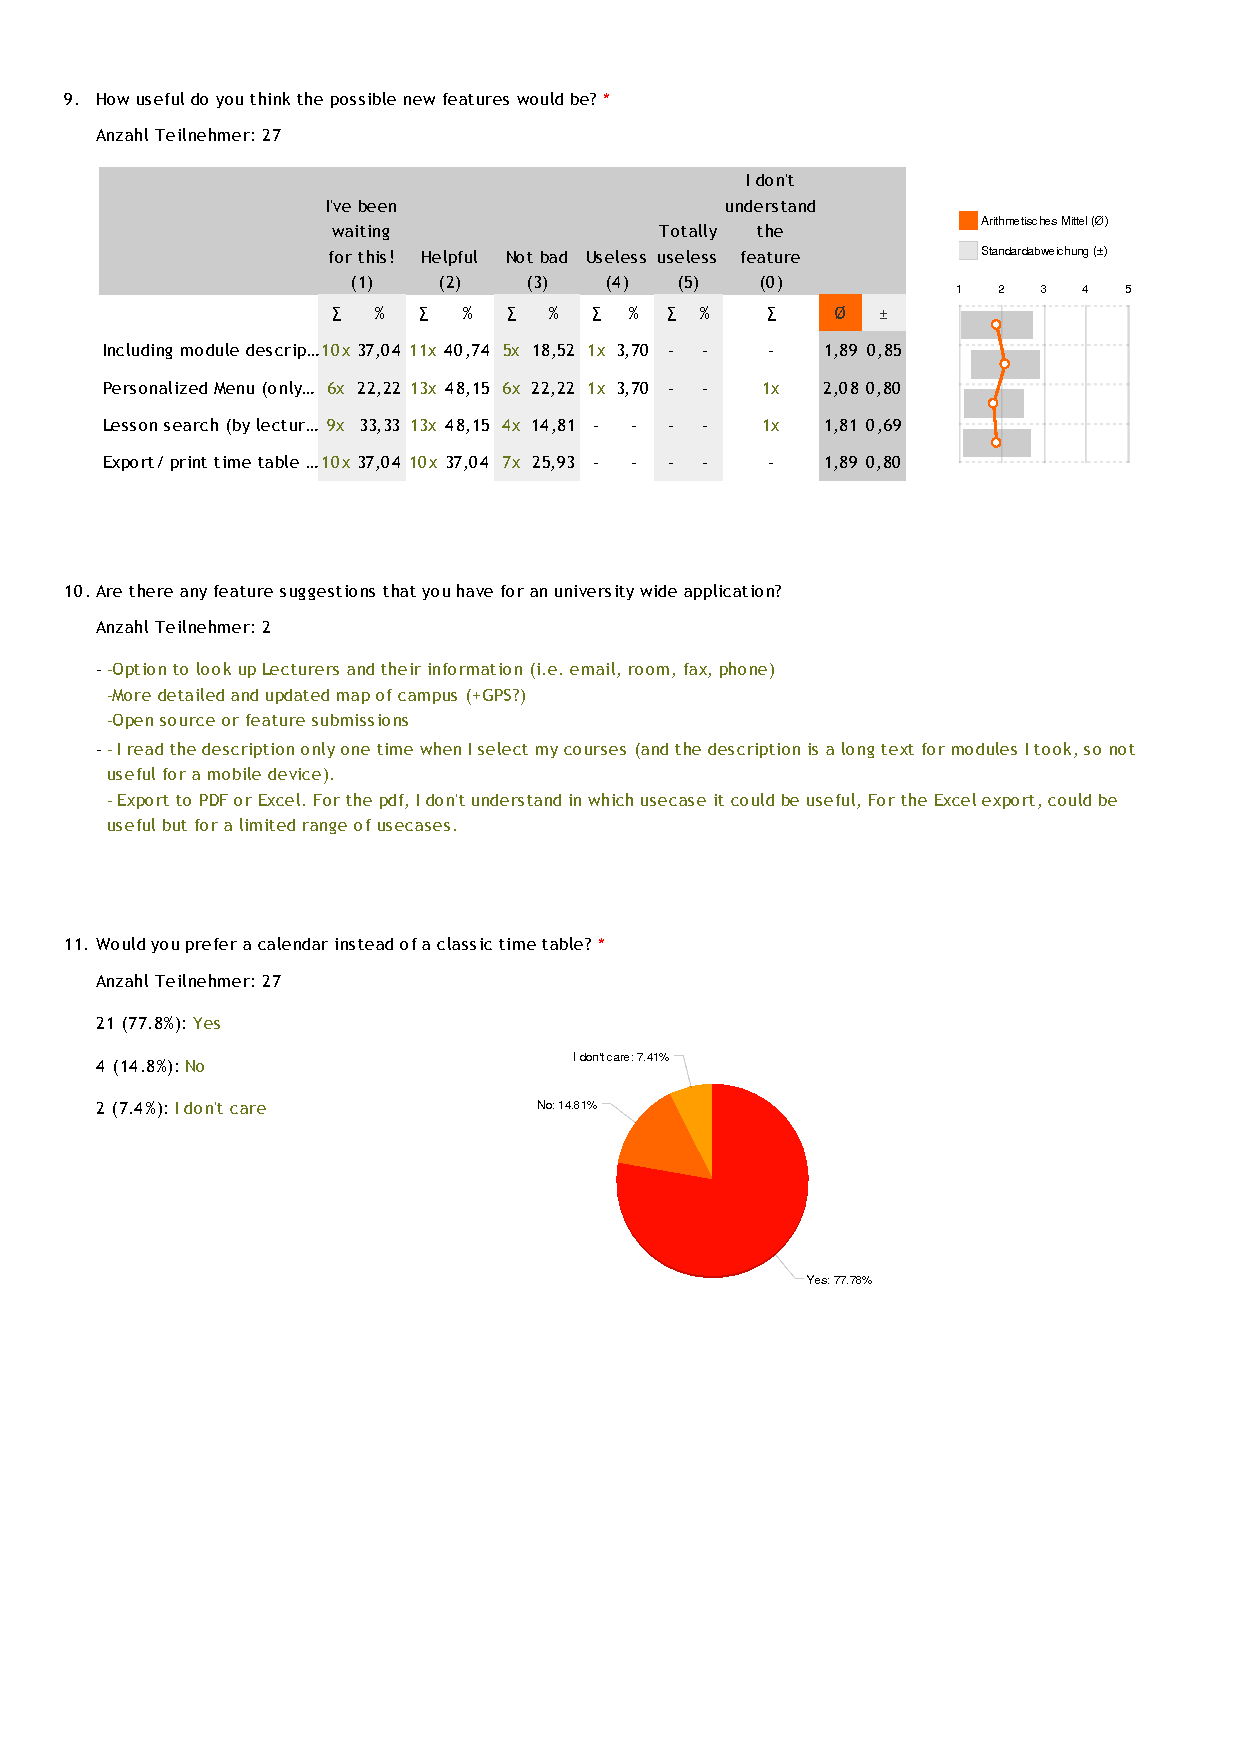
\includegraphics[
    width=\textwidth,
    height=\textheight,
    keepaspectratio
]{Kapiteln/Anhang/Inhalt/EN/survey_EN_Page5.pdf}
\vfill
\newpage
\noindent
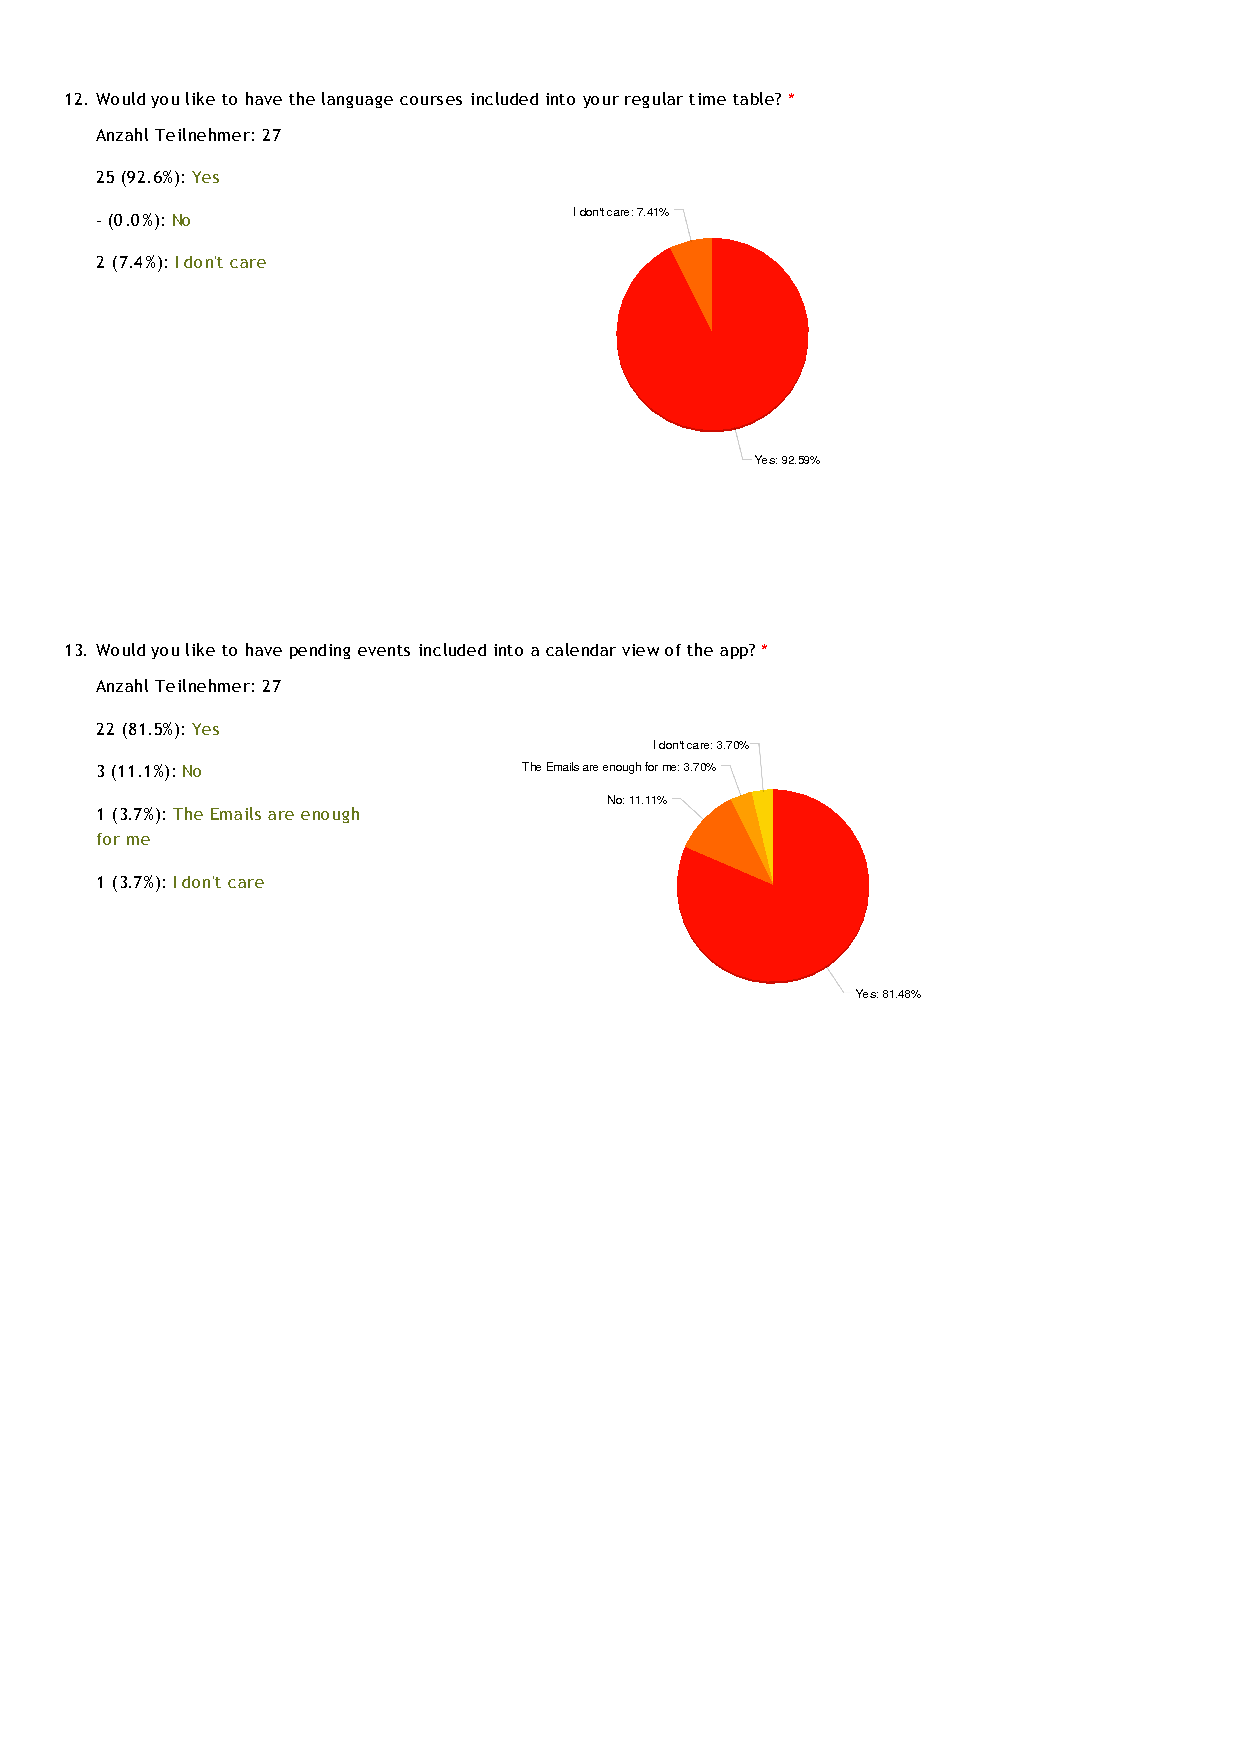
\includegraphics[
    width=\textwidth,
    height=\textheight,
    keepaspectratio
]{Kapiteln/Anhang/Inhalt/EN/survey_EN_Page6.pdf}
\vfill
\newpage
\noindent
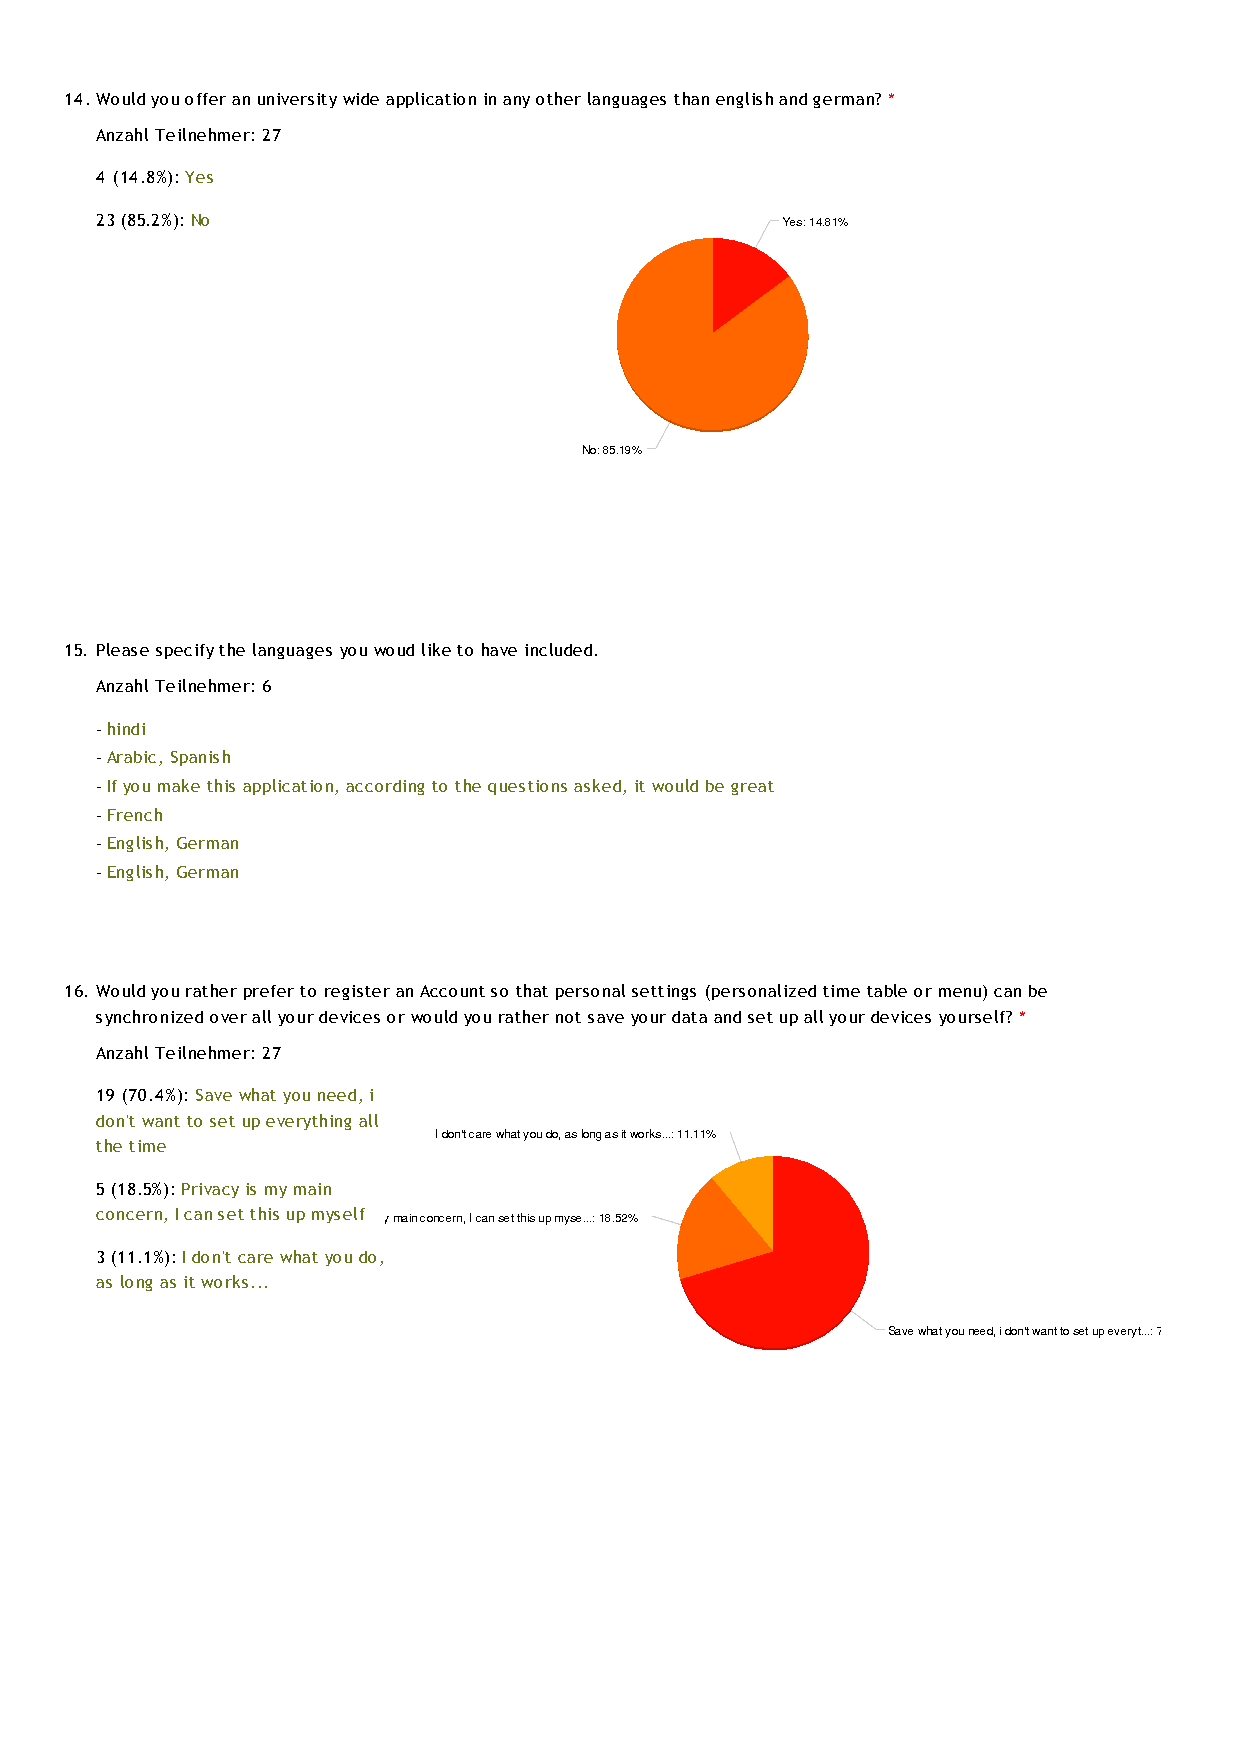
\includegraphics[
    width=\textwidth,
    height=\textheight,
    keepaspectratio
]{Kapiteln/Anhang/Inhalt/EN/survey_EN_Page7.pdf}
\vfill
\newpage
\noindent
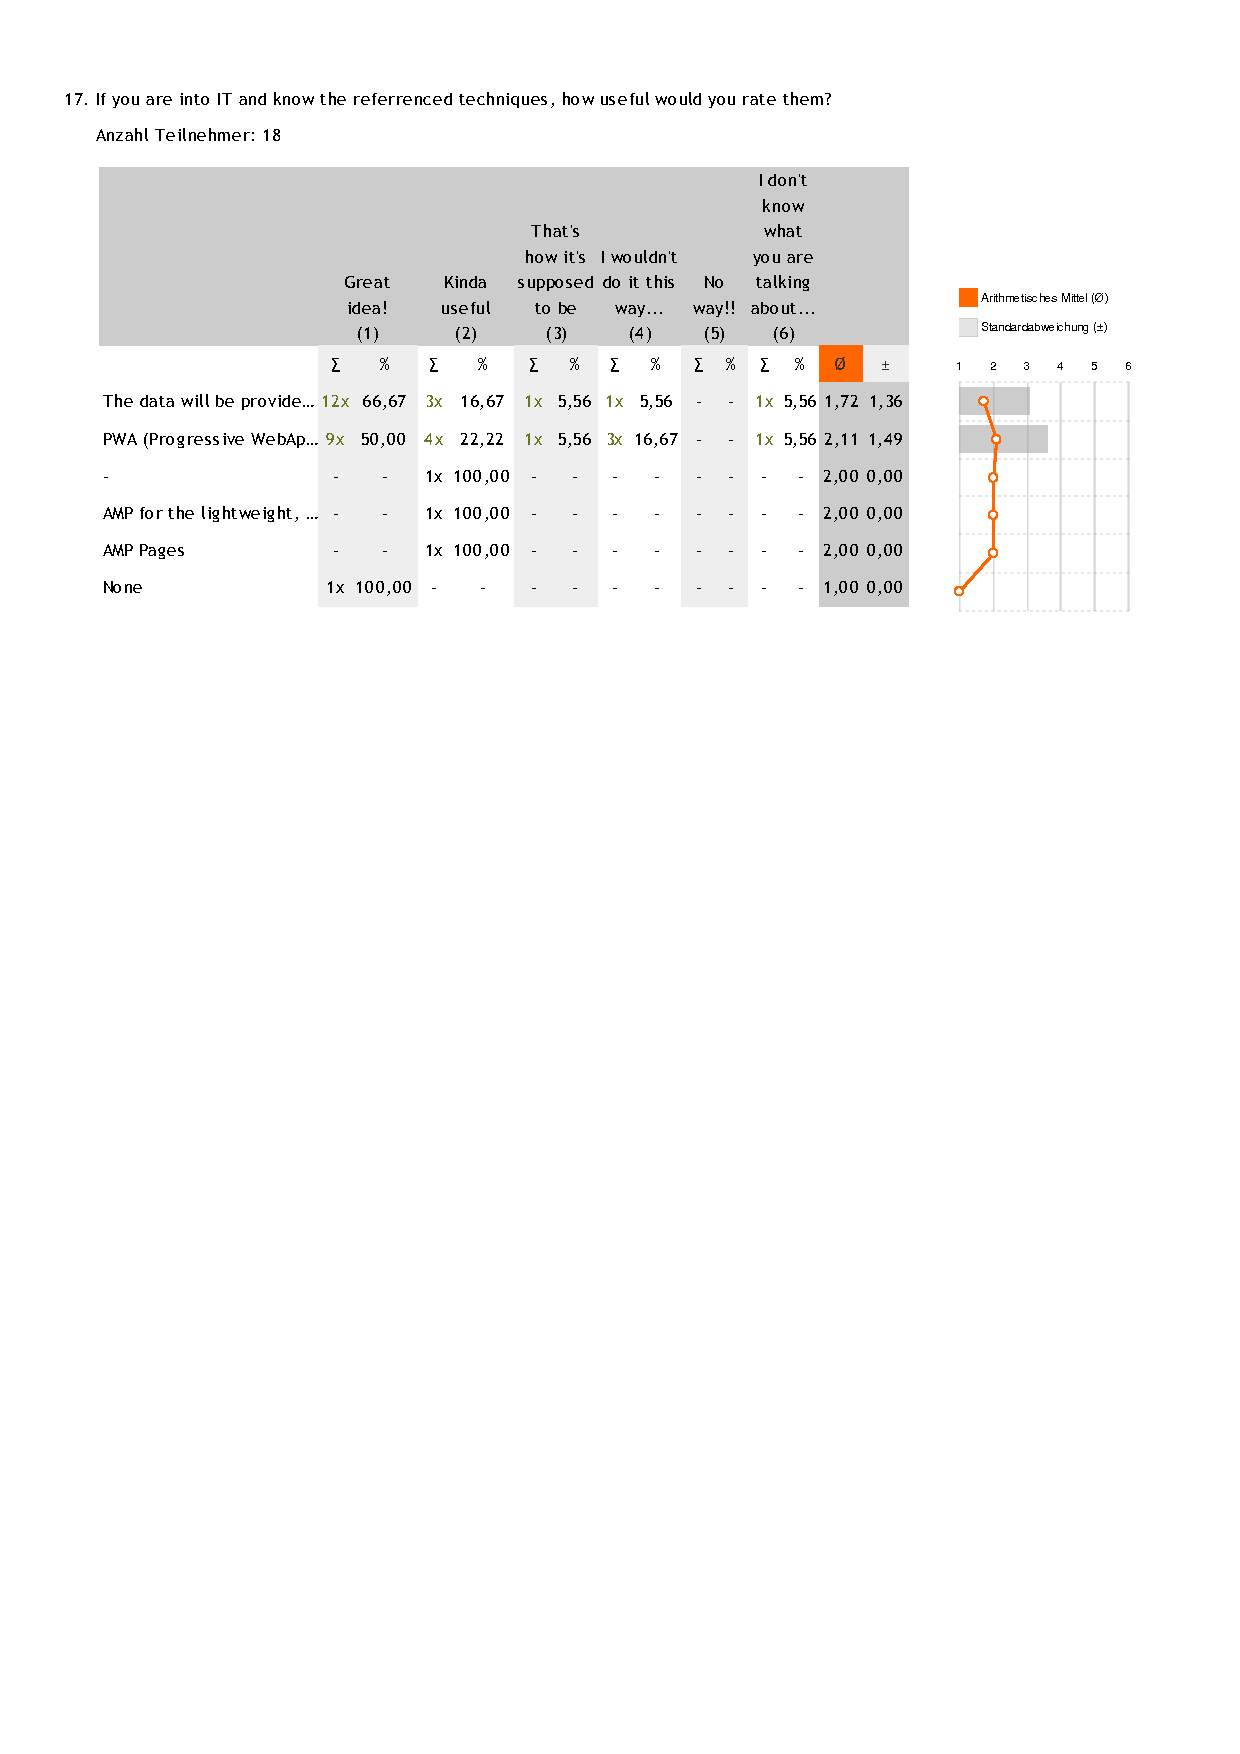
\includegraphics[
    width=\textwidth,
    height=\textheight,
    keepaspectratio
]{Kapiteln/Anhang/Inhalt/EN/survey_EN_Page8.pdf}
\vfill
\cleardoublepage

\section*{Autoren Referenz}
\addcontentsline{toc}{section}{Autoren Referenz}

Diese wissenschaftliche Arbeit ist eine Zusammenarbeit der beiden Autoren Dennis Brysiuk und Noah Lehmann. Um daher einen besseren Überblick über die Zuordnung der Inhalte zu haben wird im folgenden eine Tabelle dargestellt, die die Kapitel ihren jeweiligen Verfassern zuordnet.

\begin{table}[H]
\begin{center}
  \begin{tabular}{| l | l | l |}
 
\hline
\rowcolor{Gray}
\textcolor{white}{\textbf{Kapitel}} & \textcolor{white}{\textbf{Kapitel Bezeichnung}} & \textcolor{white}{\textbf{Autor}} \\
\rowcolor{Gray}
\textcolor{white}{\textbf{Nr.}} 	&  												  & \\  

\hline    
\rowcolor{LGray} 						
\textbf{1}		& \textbf{Einleitung}	&  				\\
\hline
1.1		& Beweggründe					& Noah Lehmann	\\
\hline
1.2		& Zielsetzung					& Noah Lehmann	\\
\hline
1.3		& Zielgruppe					& Noah Lehmann	\\
\hline
1.4		& Vorausgesetztes Wissen		& Noah Lehmann	\\
\hline
1.5		& Vorgeschlagene Nebenlektüre	& Noah Lehmann	\\

\hline    
\rowcolor{LGray} 						
\textbf{2}		& \textbf{Auswertung vorhandener Anwendungen} &  				\\
\hline
2.1		& Allgemeine Auswertung der Zufriedenheit	& Noah Lehmann	\\
\hline
2.1.1	& Zielgruppen								& Noah Lehmann	\\
\hline
2.1.2	& Ergebnisse								& Noah Lehmann	\\
\hline
2.1.3	& Fazit										& Noah Lehmann	\\
\hline
2.2		& Anwendungen								& Noah Lehmann	\\
\hline
2.2.1	& Android									& Noah Lehmann	\\
\hline
2.2.2	& iOS										& Noah Lehmann	\\
\hline
2.2.3	& Windows App								& Noah Lehmann	\\
\hline
2.2.4	& Website									& Noah Lehmann	\\
\hline
2.2.5	& Fazit										& Noah Lehmann	\\

\hline    
\rowcolor{LGray} 						
\textbf{3}	& \textbf{Funktionale Anforderungen} &  				\\
\hline
3.1		& Auftraggeber					& Noah Lehmann	\\
\hline
3.1.1	& Grundlegenden Anforderungen	& Noah Lehmann	\\
\hline
3.1.2	& Funktionale Anforderungen		& Noah Lehmann	\\
\hline
3.2		& International Office			& Noah Lehmann	\\
\hline
3.2.1	& Problem						& Noah Lehmann	\\
\hline
3.2.2	& Funktionale Anforderungen		& Noah Lehmann	\\


\hline
  \end{tabular}
  \end{center}
\caption[Autoren Referenz]{Autoren Referenz}
\label{tab:autoren}
\end{table}

\newpage

\begin{table}[H]
\begin{center}
  \begin{tabular}{| l | l | l |}
 
\hline
\rowcolor{Gray}
\textcolor{white}{\textbf{Kapitel}} & \textcolor{white}{\textbf{Kapitel Bezeichnung}} & \textcolor{white}{\textbf{Autor}} \\
\rowcolor{Gray}
\textcolor{white}{\textbf{Nr.}} 	&  												  & \\  

\hline
3.3		& Sprachenzentrum				& Noah Lehmann	\\
\hline
3.3.1	& Problem						& Noah Lehmann	\\
\hline
3.3.2	& Funktionale Anforderungen		& Noah Lehmann	\\
\hline
3.4		& Pflichtenheft					& Noah Lehmann	\\

\hline    
\rowcolor{LGray} 						
\textbf{4}	& \textbf{Architektur von Softwaresystemen}	&	\\
\hline
4.1		& Grundlegendes						& Dennis Brysiuk \\
\hline
4.2		& Nicht-funktionale Anforderungen	& Dennis Brysiuk \\
\hline
4.3		& Prinzipien						& Dennis Brysiuk \\
\hline
4.3		& Fazit								& Dennis Brysiuk \\

\hline    
\rowcolor{LGray}
\textbf{5}		& \textbf{Web Services}	&  			\\
\hline
5.1		& Serviceorientierte Architektur			& Dennis Brysiuk \\
\hline
5.1.1	& Technische Konzepte						& Dennis Brysiuk \\
\hline
5.1.2	& Zusammenfassung							& Dennis Brysiuk \\
\hline
5.2		& Webservice Arten							& Dennis Brysiuk \\
\hline
5.2.1	& Simple Object Access Protocol (SOAP)		& Dennis Brysiuk \\
\hline
5.2.2	& Representational State Transfer (REST)	& Dennis Brysiuk \\
\hline
5.2.3	& Bewertung									& Dennis Brysiuk \\

\hline    
\rowcolor{LGray}
\textbf{6}		& \textbf{REST API Design}	&  				\\
\hline
6.1		& Ressourcen Design				& Dennis Brysiuk \\
\hline
6.1.1	& Versionsverwaltung			& Dennis Brysiuk \\
\hline
6.1.2	& URI Namenskonvention			& Dennis Brysiuk \\
\hline
6.1.3	& Ressourcen Namenskonvention	& Dennis Brysiuk \\
\hline
6.1.4	& HTTP Methoden					& Dennis Brysiuk \\
\hline
6.2		& Request Struktur				& Dennis Brysiuk \\
\hline
6.2.1	& Header						& Dennis Brysiuk \\
\hline
6.2.2	& Query Parameter				& Dennis Brysiuk \\
\hline
6.2.3	& Aufteilung einer Ressource	& Dennis Brysiuk \\
\hline
6.3		& Response Handling				& Dennis Brysiuk \\
\hline
6.3.1	& Response Inhaltsformat		& Dennis Brysiuk \\
\hline
6.3.2	& HTTP Statuscode				& Dennis Brysiuk \\
\hline
6.3.3	& Asynchrone Callbacks			& Dennis Brysiuk \\
\hline
6.4		& Hypermedia					& Dennis Brysiuk \\

\hline
  \end{tabular}
  \end{center}
\caption[Autoren Referenz]{Autoren Referenz}
\label{tab:autoren}
\end{table}

\newpage

\begin{table}[H]
\begin{center}
  \begin{tabular}{| l | l | l |}
 
\hline
\rowcolor{Gray}
\textcolor{white}{\textbf{Kapitel}} & \textcolor{white}{\textbf{Kapitel Bezeichnung}} & \textcolor{white}{\textbf{Autor}} \\
\rowcolor{Gray}
\textcolor{white}{\textbf{Nr.}} 	&  												  & \\  

\hline    
\rowcolor{LGray} 						
\textbf{7} & \textbf{Architektur Hochschul-App} &  				\\
\hline
7.1		& Serviceorientierte Architektur	& Dennis Brysiuk \\
\hline
7.2		& Microservice Architektur			& Noah Lehmann \\
\hline
7.3		& Schichtenarchitektur				& Noah Lehmann \\

\hline    
\rowcolor{LGray} 						
\textbf{8} & \textbf{Services der Hochschul-App}	&  				\\
\hline
8.1		& Stundenplan (Timetable-Service)			& Noah Lehmann \\
\hline
8.2		& Planänderungen (Timetable-Change-Service)	& Noah Lehmann \\
\hline
8.3		& Speiseplan (Mensa-Service)				& Dennis Brysiuk \\
\hline
8.4		& Benachrichtigungen (Notification Service)	& Dennis Brysiuk \\
\hline
8.5		& Sicherheit (Auth-Service)					& Dennis Brysiuk \\
\hline
8.6		& Anwenderverwaltung (User-Service)			& Dennis Brysiuk \\
\hline
8.7		& Weitere Dienste							& Noah Lehmann \\

\hline    
\rowcolor{LGray} 						
\textbf{9} & \textbf{Ausblick und Fazit} &  				\\
\hline
9.1		& Ausblick						& Noah Lehmann \\
\hline
9.2		& Weitere Bachelorarbeitsthemen	& Noah Lehmann \\
\hline
9.3		& Fazit							& Noah Lehmann \\
\hline

\hline
  \end{tabular}
  \end{center}
\caption[Autoren Referenz]{Autoren Referenz}
\label{tab:autoren}
\end{table}

\cleardoublepage

%Abstand Verzeichnisse
\renewcommand*{\chapterheadstartvskip}{\vspace*{0cm}}

%Literaturverzeichnis
\cleardoublepage
\printbibliography[heading=bibintoc,nottype=online,title={Literaturverzeichnis}]
\cleardoublepage
\printbibliography[type=online,title={Internetquellen}]

\chapter*{Eidesstattliche Erklärung}
\addcontentsline{toc}{chapter}{Eidesstattliche Erklärung}
Ich erkläre hiermit, dass ich meinen Beitrag zur vorliegenden Gruppenarbeit (Kapitel 4, 5, 6, 7.1, 8.3, 8.4, 8.5, 8.6)
selbständig und ohne Benutzung anderer als der angegebenen Hilfsmittel angefertigt habe; das gleiche gilt für die von den auf dem Titelblatt der Arbeit genannten Autoren gemeinsam verfassten Teile (Kapitel 1, 2, 3, 7.2, 7.3, 8.1, 8.2, 8.7, 9). 
Die aus fremden Quellen direkt oder indirekt übernommenen Gedanken sind als solche kenntlich gemacht.\\
\linebreak
Die Arbeit wurde nach meiner besten Kenntnis bisher in gleicher oder ähnlicher Form keiner anderen Prüfungsbehörde vorgelegt und auch noch nicht veröffentlicht.\\
\linebreak
\linebreak
\linebreak
Hof, den 03.12.2019


%(Kapitel 4, 5, 6, 7.1, 8.3, 8.4, 8.5, 8.6) %Dennis
%(Kapitel 1, 2, 3, 7.2, 7.3, 8.1, 8.2, 8.7, 9) %Noah

\thispagestyle{empty}
\newgeometry{left=2.5cm, right=2.5cm, bottom=2.5cm, top=2.5cm}

\section*{Abstract}
Die vorliegende Bachelorarbeit zielt darauf ab, die Analyse für eine zukunftsfähige, beständige und erweiterbare Hochschulapp bereitzustellen. Um eine solide Grundlage dafür zu schaffen, werden in dieser Arbeit ebenfalls bestehende Anwendungen zur Informationsbeschaffung der Hochschule Hof analysiert und die Nutzergruppen zu deren Präferenzen  befragt. Aus den gewonnenen Ergebnissen werden dann die Anforderungen gesammelt und anhand derer die finalen Entwürfe der Anwendung gefertigt und gerechtfertigt.\\
Der erste Teil der Arbeit befasst sich lediglich mit der Analyse der vorhandenen plattformgebundenen Anwendungen der Hochschule Hof, unter anderem der Android App, der iOS App aber auch mit der klassischen Website der Hochschule Hof. Es werden die Funktionen gesammelt und analysiert. Danach werden die Nutzer der Apps, die Studierenden der Hochschule Hof, zu den bestehenden Anwendungen befragt. Anhand der gewonnenen Erkenntnisse können die gewünschten Funktionen dann gesammelt und bewertet werden.\\
Mit den Informationen aus dem ersten Teil der Arbeit werden dann die Anforderungen an die Arbeit gesammelt. Dabei wird nicht nur der Auftraggeber mit einbezogen, sondern auch andere Interessengruppen, genauer das International Office und das Sprachenzentrum der Hochschule Hof. Zu den wichtigsten Anforderungen kommt die Plattformunabhängigkeit der Anwendung und die Internationalisierung in Form von Mehrsprachigkeit im Einklang mit dem Leitbild der Hochschule Hof. Zu den Anforderungen wird außerdem ein referenzierbares Lastenheft angefertigt.\\
Um die nicht funktionalen Anforderungen wie Erweiterbarkeit und Modularität gerecht zu werden, wird im Mittelteil der Arbeit der Fokus auf einige Prinzipien und Designphilosophien der Softwarearchitektur gelegt. Hier werden Ideen wie das KISS-Prinzip, Serviceorientierte Architektur und REST  genauer betrachtet, teils auch mit Alternativen verglichen, um die passende Lösung für einen Prototypen einer neuen Hochschul-App zu finden. Durch die Identifizierung RESTful Webservices als Architekturgrundlage wird im Anschluss an die Sammlung der Paradigmen ebenfalls ein Regelwerk für das Arbeiten mit REST festgelegt.\\
Abschließend wird konkret an der Lösung der Hochschul-App gearbeitet. Hierfür wird erst die grundlegende Architektur angerissen und genauer erläutert. Lösungen wie Discovery Services und API-Gateways werden dort genauer erläutert. Abschließend wird dann der konkrete Aufbau der Microservice Architektur erklärt. Hierbei werden nicht nur die Ressourcen definiert, es wird auch auf die darunterliegende Logik und den Datenbankkonzepten eingegangen.\\
Zusammenfassend erarbeitet diese Bachelorarbeit den konkreten Prototypen der Hochschul-App in allen Phasen der Analyse. Durch die Ideen aus den vorhandenen Anwendungen und dem Feedback der Nutzer konnten die Anforderungen gesammelt werden. Aus diesen Anforderungen konnten dann die nötigen Architekturprinzipien identifiziert werden und daraus resultierend die passende Architektur gefunden werden. Aufbauend auf der Architektur konnten dann die Feinheiten der App ausgearbeitet werden.

\end{document}
